%                                                                 aa.dem
% AA vers. 9.1, LaTeX class for Astronomy & Astrophysics
% demonstration file
%                                                       (c) EDP Sciences
%-----------------------------------------------------------------------
%
%\documentclass[referee]{aa} % for a referee version
%\documentclass[onecolumn]{aa} % for a paper on 1 column  
%\documentclass[longauth]{aa} % for the long lists of affiliations 
%\documentclass[letter]{aa} % for the letters 
%\documentclass[bibyear]{aa} % if the references are not structured 
%                              according to the author-year natbib style
%
\documentclass{aa}  

%
\usepackage{graphicx}
%%%%%%%%%%%%%%%%%%%%%%%%%%%%%%%%%%%%%%%%
\usepackage{txfonts}
%%%%%%%%%%%%%%%%%%%%%%%%%%%%%%%%%%%%%%%%
\usepackage{hyperref}
% To add links in your PDF file, use the package "hyperref"
% with options according to your LaTeX or PDFLaTeX drivers.
%
%%%%%%%%%%%%%%%%%%%%%%%%%%%%%%%%%%%%%%%%%
\usepackage[usenames, dvipsnames]{color}
\usepackage{overpic} % add text to fig


% NOTATION
%%%%%%%%%%%%%%%%%%%%%%%%%%%%%%%%%%%%%%%%%
\newcommand{\hls}{HLS\,J0918+5142}
\newcommand{\ftone}{f_{\rm{tone}}}
\newcommand{\am}{x}
\newcommand{\elev}{\delta}
\newcommand{\nika}{NIKA2}
\newcommand{\aka}{a.\,k.\,a.}
\newcommand{\wrt}{w.\,r.\,t.}
\newcommand{\bm}{{\tt beammap}}
\newcommand{\bms}{{\tt beammaps}}
\newcommand{\rf}{\emph{RfdIdQ}}
\newcommand{\kidpar}{\emph{kidpar}}
\newcommand{\radec}{\emph{R.\,A.,\,Dec}}
\newcommand{\cm}{\emph{common~mode}}
\newcommand{\cmoneb}{\emph{common~mode~one~block}}
\newcommand{\afternoon}{temperature-induced}
\newcommand{\Afternoon}{Temperature-induced}

% COMMENTS
%%%%%%%%%%%%%%%%%%%%%%%%%%%%%%%%%%%%%%%%%%%
\newcommand{\todo}[1]{ {\color{magenta} $[$ TO DO: $]$ #1} }


\begin{document} 


   \title{NIKA2 Calibration and Performance at the IRAM 30-m Telescope}

   \author{Laurence Perotto
     \inst{1}
     \and
     Others ToBeDiscussed
%     Nicolas Ponthieu
%     \inst{2}
%     \and Juan-F. Mac\'ias-P\'erez
%     \inst{1}
%     \and 
%     F.-Xavier D\'esert
%     \inst{2}
%     \and 
%     Jean-Fran\c cois Lestrade
%     \inst{3}
%     \and
%     Herv\'e Aussel
%     \inst{4}
%     \and
%     Fr\'ed\'eric Mayet
%     \inst{1}
%     \and
%     Florian Ruppin
%     \inst{1}
     \and
     NIKA2 CORE TEAM
   }

   \institute{Univ. Grenoble Alpes, CNRS, Grenoble INP, LPSC-IN2P3, 53, avenue des Martyrs, F-38000 Grenoble, France \\
     \email{laurence.perotto@lpsc.in2p3.fr}
    % \and
    % Univ. Grenoble Alpes, CNRS, IPAG, F-38000 Grenoble, France\\
    % \and
    % LERMA, Observatoire de Paris, PSL Research University, CNRS, Sorbonne Universités, UPMC Univ. Paris 06, F-75014, Paris, France\\
    % \and
    % AIM, CEA, CNRS, Universit\'e Paris-Saclay, Universit\'e Paris Diderot, Sorbonne Paris Cit\'e, F-91191 Gif-sur-Yvette, France
   }

   \date{Received April XX, 2019; Accepted XXXX XX, 2019}

% \abstract{}{}{}{}{} 
% 5 {} token are mandatory
   
   \abstract
   % context heading (optional)
   % {} leave it empty if necessary  
       {The New IRAM KID Array, NIKA2, is a dual-band millimetric
         camera of thousands of Kinetic
         Inductance Detectors (KID) installed at the IRAM 30-meter
         telescope at Pico Veleta (Spain). The instrument
         commissioning  was successfully completed in September
         2017. NIKA2 is now open to the scientific community and will
         operate for the next decade. NIKA2 will be a key experiment for a vast variety of
         astrophysic and cosmology purposes, including planet
         formation, star formation in the Milky Way, gas in
         nearby galaxies, galaxy formation at high redshift and
         cosmology with galaxy clusters. The success of this ambitious science
         program will depend on the accuracy of the calibration and
         its stability againts observing conditions.}
       % aims heading (mandatory)
       {We present the methods that have been developped for NIKA2
         calibration and their application to the first year of final
         set-up operation to assess the on-sky performance.}
       % methods heading (mandatory)
       {We used several
         thousands of observation scans that were acquired at the February
         2017 technical campaign, during which NIKA2 instrumental set-up was
         in the final configuration for the first time,
         and at the first science pools that took place in October 2017 and
         January 2018. This vast data set allows us to check the performance
         stability for one year and against a large range of observing
         elevations and atmospheric conditions. %The calibration and
         %performance assessment methods that we have developed are also
         %thoroughly described, as well as the robustness tests that we have
         %performed.
       }
       % results heading (mandatory)
       {We find an average fraction of usable detectors during a
         typical observing scan of 84 per cent in the 260~GHz bands and 90 per cent in the
         150~GHz, which well cover the 6.5 arcmin diameter field of
         view. The beam pattern has been measured and is characterized
         by a full width at half maximum (FWHM) of $11.1\pm0.1$ arcsec
         and $17.6 \pm 0.1$, and a beam efficiency of $55\pm 3$ and
         $77\pm 2$ per cent at 260 and 150~GHz respectively. The
         statistital relative calibration uncertainties are of about 6
       and 3 per cent for these two frequency bands, which validates
       the accuracy of the method we have deployed to correct for the
       atmosphere attenuation. The top-of-atmosphere noise equivalent
       flux density (NEFD) at 260 and 150~GHz are of $30 \pm 3$ and
       $9 \pm 1$ mJy.s$^{1/2}$/beam. This state-of-the-art performance
       confers NIKA2 with excellent mapping capabilities characterized
       by mapping speeds of about 100 and 1400
       arcmin$^2$/hours/mJy$^2$ at 260 and 150~GHz.}
       % conclusions heading (optional), leave it empty if necessary 
       {}

   \keywords{Submillimeter, Photometry, Method: observational, Cosmology: Cosmic Microwave Background}

   \maketitle

   
%----------------------------------------------------------------------------------------
%	1./ INTRODUCTION
%----------------------------------------------------------------------------------------
\section{Introduction}
\label{se:intro}
%----------------------------------------------------------------------------------------
%	INTRODUCTION
%----------------------------------------------------------------------------------------
%\section{Introduction}
%\label{se:intro}
%
%Submillimetric domain: a unique thorough view of the Universe from
%planetary surfaces in the Solar System to early galaxies,
%high-redshift galaxy clusters and the Cosmic Microwave
%Background (CMB).\\
%Ground-based submillimeter experiments have made tremendous progress in the last
%decades thanks to the advent of large detector arrays, challenging the
%motivation for spatial experiments.\\
%The current experimental efforts are driven by two complementary
%challenges: the improvement of the polarisation sensitivity to detect
%primordial polarisation B-mode of the CMB and measure CMB lensing on
%one hand and on the other hand the increase the angular resolution to
%reveal the inner structure of astrophysical objects, such as
%high-redshift galaxies and galaxy clusters.\\

Submillimetric and millimetric domains offer a unique view on the
Universe from nearby astrophysical objects, including planets,
planetary systems, galactic sources, nearby galaxies, to high-redshift
cosmological probes, \emph{e.g.} distant dusty star-forming galaxies,
clusters of galaxies, Cosmic Infrared Background (CIB), Cosmic Microwave
Background (CMB).
%for scientific purposes that ranges from planetary science to cosmology.

Ground-based {\lp continuum} millimeter experiments have made spectacular progress in
the past-two decades thanks to the advent of large arrays of
high-sensitivity detectors~\citep{Wilson2008_AZTEC,
  Siringo2009_LABOCA, Swetz2011_ACT, Bleem2012_SPT, Monfardini2011_NIKA, Holland2013_SCUBA2,
  Dicker2014_MUSTANG2, Adam2017}. %, challenging the
%motivation for spatial experiments.
This fast grow will continue as experimental efforts are
driven by two challenges: improving the sensitivity to the
polarisation to detect the signature of
the end-of-inflation gravitational waves in the CMB, and reaching
arcminute angular resolution to exploit the CMB secondary anisotropies
as cosmological probes, and sub-arcminute resolution to unveil the
inner structure of faint or complex astrophysical objects and to map
the early universe down to the confusion limit. Furthermore, new
generation of sub-arcminute millimetric experiments, like NIKA2, which
combines high angular resolution with a high mapping speed and a large
coverage in the frequency domain, will achieve a breakthrough in 
%will revolutionize
our detailed understanding of the formation and evolution of
structures throughout the Universe.

%
%In particular, it would allow us to study the inner structure of
%galaxy clusters (detected by Planck), and to get a new view on star
%formation at low and high redshift, by studying the role of magnetic
%field at a sub parsec scale in our Galaxy, and mapping the dusty star
%forming galaxies up to redshifts equal to 6.
%
%NIKA2 is a high-resolution large field-of-view multi-thousand detector
%camera in operation at the 30-m IRAM telescope since October 2017. ,
%after a successful commissioning of the instrument. 
%Fourth generation of
%imagers installed at the IRAM 30-m: after the single beam
%imagers, the 7-pixel camera of the late 90's and several versions of
%MAMBO. Unlike its predecessors, NIKA2 is based on KIDs. Validated with
%NIKA pathfinder.\\
%Brief historic of the commissioning. \\
%The instrument commissioning was successfully completed in September
%2017.
%NIKA2 is now open to the scientific community and will operate
%for the next decade.

The New IRAM KID Array Two, NIKA2, is a subarcminute-resolution
high-mapping speed camera observing simultaneously a 6.5' diameter
field of view (FOV) in intensity in two
frequency channels centered at 150 and $260\,\rm{GHz}$ and in
polarisation at $260\, \rm{GHz}$. NIKA2 was installed at the
30-meter IRAM telescope in October 2015 with a partial readout
electronics, and operated in the final instrumental configuration since
January 2017. After a successful
commissioning phase that ended in October 2017, NIKA2 is
open to the community for science-purpose observations for the next
decade. NIKA2 will provide key observations both at the galactic scale
and at high redshifts to address a plethora of open questions, including
the environment impact on dust properties, the star formation process
at low and high redshifts, the evolution of the large-scale structures
and the exploitation of galaxy clusters for accurate cosmology.
%
%NIKA2, which will provide unprecedented maps at low and high
%redshifts, ranging from the interstellar medium to the dusty star
%forming galaxies up to redshifts equal to 6, will be a key experiment
%to address plethora of open questions in astrophysic and cosmology,
%ranging from the understanding of the star formation process at low
%and high redshift to  and accurate cosmology with galaxy clusters 
%

At the galactic scale, progress in understanding the star formation
process relates to an accurate characterisation of dust properties in
the interstellar medium (ISM). NIKA2 will provide the high-resolution
high-mapping speed dual-wavelength millimeter observations that are
required for the determination of the mass and emissivity of
statistically significant samples of dense, cold, star-forming
molecular clouds~\citep{Rigby2018}.
Deep multi-wavelengths surveys of nearby galaxies and of large areas
of the galactic plane also allows for setting constraints on
environmental-related variations of the dust properties.
Furthermore, NIKA2 observations are needed for a
detailed study of the inner molecular cloud filamentary structure that
hosts Solar-mass star progenitors~\citep{Bracco2017}, to
understand the evolution process that culminates in star
formation (see \emph{e.g.}~\citet{Andre2014} for a review). Ultimately, these
observations are also helpful to understand planet formation within
protoplanetary disks.

For cosmology, NIKA2 observations will have two major
implications. On the one hand, they represent a unique opportunity to
study the evolution of the galaxy cluster mass calibration with
redshift and {\lp dynamical state} for their accurate exploitation as cosmological probe. 
Galaxy clusters are efficiently detected via the thermal
Sunyaev-Zel'dovich (tSZ) effect up to high redshifts {\lp ($z<1.5$)}, as was recently
proven by CMB
experiments~\citep{Hasselfield2013_ACT_SZ, Reichardt2013_SPT_SZ, Planck2016_SZcat}.
The exploitation of the vast SZ-selected galaxy cluster catalogues is
currently the most powerful approach for cosmology with galaxy
clusters~\citep{Planck_2016_SZ_cosmo}. However, the accuracy of the tSZ cluster
cosmology relies on the calibration of the relation between the tSZ
observable and the cluster mass and on the assessment of both the redshift
evolution and the impact of the complex cluster physics. 
%Cosmological constraints can be drawn from tSZ-selected cluster
%samples by using either the cluster number counts or the angular power
%spectrum. It requires a high purity sample to avoid bias, and in
%particular the understanding of the distribution of matter within the
%cluster, and the evaluation of the scatter induced by disturbed
%systems in the relation between the tSZ integrated flux and the total
%cluster mass.
Previous arcminute resolution experiments only allowed detailed studies
of the intra cluster medium spatial distribution for low redshift clusters (z <
0.2). Sub-arcminute resolution high mapping speed experiments are
required to extend our understanding of galaxy cluster towards high
redshift. \citet{Ruppin2018} has reported the first high-resolution
tSZ mapping of a galaxy cluster with NIKA2. Furthermore, NIKA2
capabilities for the characterization of high-redshift {\lp ($0.5<z<0.9$)} galaxy clusters
has been verified using numerical simulation~\citep{Ruppin2019}.

On the other hand, in-depth mapping of large extragalactic fields with
sub-arcminute resolution with NIKA2 will provide unprecedented insight
on the distant universe. %Combining high mapping speed and sub-arminute
%resolution is mandatory to
Indeed, hundreds of dust-obscured optically-faint galaxies will be
detected up to high redshift
($z \approx 5$) during their major episodes of star formation.
%For this
%purpose, the high-angular resolution, combined with high mapping
%speed, is key to reduce the confusion noise, which is the ultimate
%limit of cosmological surveys~\citep{Bethermin2017_simu}.
{\lp For this purpose, the high-angular resolution is key to reduce the
confusion noise, which is the ultimate limit of cosmological
surveys~\citep{Bethermin2017_simu}, while the high mapping speed allows
this irreducible noise level to be reached in the extragalactic field
map in a short integration time.}
This will help quantifying the star formation at $z \approx 5$, probing the whole
star formation evolution across cosmic ages and clarifying the
role of the dusty galaxies in the reionization of the
universe~\citep{Mancuso2016}. Moreover, NIKA2 observations will be critical for our
understanding of galaxy formation and evolution.

%[ATTENTION COPIE]
%Similarly, distant universe studies via deep surveys will
%benefit from a large instantaneous field-of-view and sensitivity
%to cover sky regions at the confusion limit. This results
%in detecting dust-obscured optically faint galaxies during
%their major episodes of star formation in the early universe
%(B\'ethermin et al. 2017, Geach et al. 2017).\\

The current generation of sub-arcminute resolution experiments also
include the Large APEX Bolometer Camera
(LABOCA~\citep{Siringo2009_LABOCA}) at the Atacama
Pathfinder Experiment (APEX) 12-meter telescope, which covers a
12' diameter FOV at $345\, \rm{GHz}$ {\lp at an angular resolution of about
19''}; AzTEC at the 50-meter Large Millimeter Telescope, which operates with a
single bandpass centered at either 150, 220 or
$270\,\rm{GHz}$~\citep{Wilson2008_AZTEC}, {\lp and which has a beam FWHM of
$18''$ in the latter band}; the Submillimeter Common User Bolometer
Array Two (SCUBA-2~\citep{Holland2013_SCUBA2,Dempsey2013_SCUBA2}) on the
15-meter James Clerk Maxwell Telescope, which simultaneously
images a FOV of about 7' %at $850\, \mu\rm{m}$ ($353\,
%\rm{GHz}$) and $450\, \mu\rm{m}$
%($666\,\rm{GHz}$)
at $353\,\rm{GHz}$ and $666\,\rm{GHz}$ {\lp with a main beam FWHM of 13''
and 8'' in the two frequency channels, respectively}
; MUSTANG-2 at the 100-meter Green Bank telescope,
which maps a 4.35' FOV at 
$90\,\rm{GHz}$ {\lp with 9'' resolution}~\citep{Dicker2014_MUSTANG2, Stanchfield2016_MUSTANG2}.
Therefore, NIKA2 is unique
in combining an angular resolution better than 20'', an instantaneous FOV of a
diameter of 6.5' and multi-band observation capabilities at $150$ and
$260\,\rm{GHz}$.


Most of these instruments consists of bolometric cameras. By contrast,
NIKA2 is based on the Kinetic Inductance Detectors (KID)
technology~\citep{Day2003, Doyle2008_LEKID, Shu2018_LEKID}. This concept has been
first demonstrated with a pathfinder instrument,
NIKA~\citep{Monfardini2010_NIKA, Monfardini2011_NIKA}.
Installed at the IRAM 30-m telescope until 2015, NIKA demonstrated
state-of-the-art performance~\citep{Catalano2014}, and obtained
breakthrough results
(see \emph{e.g.},~\citet{Adam2014, Adam2017_kSZ}.
NIKA has been crucial in optimizing the NIKA2 instrument and data
analysis. 

%Key tool for a large variety of astrophysical and cosmological
%purposes, from Kuiper Belt objects or moons in the Solar system to
%high-redshift galaxies and galaxy clusters. The main scientific
%obsjectives are articulated around five ambitious guaranteed-time
%large programs [add a small paragraph per LP]\\
%
%These scientific program requires high performance standard in term of
%mapping capabilities, sensitivity, angular resolution and stability of
%the system. We assess this performance using a large amount of
%technical and science-purpose data acquired since the full
%installation of NIKA2.\\

A thorough description of the NIKA2 instrument is found in \citet{Adam2018},
along with the results of the commissioning in intensity based on the
data acquired during the two technical campaigns of 2017.
%
{\lp In the present paper, we propose a standard calibration method, which is
referred to as the \baseline\ calibration, to go from raw data to
stable and accurate flux density measurements.} 
%
%The present paper discusses in detail step-by-step data reduction,
%from the observations and raw data to the sensitivities and an
%assessment of the calibration accuracy, thereby discussing the pros
%and cons of different strategies to provide robust results.
%
%In this paper, we
%detail the dedicated procedures that we have developed for the
%calibration.
%We describe a standard calibration method, which is
%referred to as the \baseline\ calibration, but we are also discussing
%the pros and cons of alternative methods, which may in fact in the
%future lead to even better calibration accuracy and stability.
Furthermore we assess the performance in intensity using a large
amount of data acquired between January 2017 and February 2018.
Regarding the performance of the polarization capabilities, their
assessment will be addressed in a forthcoming paper.
To achieve a reliable and high-accuracy estimation
of the performance, we perform extensive testing of the
stability along both the analysis methodological
choices and the observing conditions.
{\lp First, the methodological choices and hypothesis may have an impact on
the performance results and the systematic errors. At each step of the
calibration procedure and for each performance metrics, we compare the
results obtained using the \baseline\ method to alternative approaches to
ensure the robustness against systematic effects.}
Second, we check the stability of the results using a large number of
independent data sets corresponding to variable observing conditions.
%To achieve
%high-accuracy estimation of each key performance characteristics,
%we test their stability against the methodological choices by
%comparing various analysis approaches, and we check their stability
%againts the observating conditions using vast independent data sets.
Specifically, most of the performance assessment relies on data
acquired during the February 2017 technical campaign (N2R9) and the
October 2017 (N2R12) and January 2018 (N2R14) first and second
scientific-purpose observation campaigns. {\lp These observation
campaigns are referred to as the {\emph reference observation campaigns}.}
Each campaign consists of about 1300 observation scans lasting between
two and twenty minutes for a total observation time of about 150 hours. 
%This large data set
%acquired through a year enables for testing against time-evolution and
%observing-dependency of the performance.

%Outlines
This paper constitutes a review of NIKA2 calibration and
performance assessment in intensity. It is intended to be a reference
for the observations with NIKA2, which will last at least ten years. 
The outline is as follows:
Sect.~\ref{se:instru}~to~\ref{se:dataproc} give short summaries of the
instrumental set up, the observational modes and the data analysis methods
that have been used for the calibration and the performance
assessment. Sect.~\ref{se:geometry}~to~\ref{se:sensitivity} detail the
dedicated calibration methods, extract the key characteristic results
and discuss their accuracy and robustness. The field-of-view
reconstruction and the KID selection for science purpose are discussed
in Sect.~\ref{se:geometry}. The beam pattern is characterised in
Sect.~\ref{se:beam}, along with the main beam
full-width at half maximum and the beam
efficiency. Sect.~\ref{se:opacity} is dedicated to the derivation of
the atmospheric opacity. The methods that we have proposed to
calibrate are gathered in Sect.~\ref{se:calibration}, while
Sect.~\ref{se:photometry} presents the validation of these methods and
the calibration accuracy and stability assessment. The noise
characteristics and the sensitivity are discussed in
Sect.~\ref{se:sensitivity}. Finally, Sect.~\ref{se:summary} summarizes
the main measured performance characteristics and {\lp briefly
describes the next steps to further improve NIKA2.}
%offers perspectives for their improvements. 


















%----------------------------------------------------------------------------------------
%	2./ INSTRUMENT
%----------------------------------------------------------------------------------------
\section{General view of the instrument}
\label{se:instru}

\section{Overview of the NIKA2 instrument}% {\color{YellowGreen} Nico}}

NIKA2 is a millimeter camera able to simultaneously image a field-of-view of
6.5\,arcmin in diameter at 150 and 260~GHz, with polarimetric capabilities at
260~GHz. The optics of the telescope receiver cabin have been modified in order
to increase the telescope field-of-view compared to earlier IRAM instruments. To
achieve these goals without degrading the telescope angular resolution, it
employs a total of around 2,900\,detectors split over three distinct arrays of
Kinetic Inductance Detectors (KID). A KID is a planar superconducting resonator
properly designed to absorb the incoming radiation and at the same time
incarnate the multiplexing scheme. The quality factors of the KID used in NIKA2
are of the order of 15,000\todo{TODO: define the 'quality factor'}.
The measurable quantity, proportional to the
incoming power per pixel, is the shift in frequency of each resonance
(pixel). This shift is a consequence of variations of the resonator (kinetic)
inductance with incoming radiation.

\subsection{Optics}

The NIKA2 camera optics include two cold mirrors, and the filtering of unwanted
(off-band) radiation is provided by a suitable stack of multi-mesh filters
placed at all temperature stages between 150 mK and room temperature. An air-gap
dichroic splits the 150\,GHz (reflection) from the 260\,GHz (transmission)
beams. A grid polariser ensures then the separation of the two linear
polarizations on the 260\,GHz channel (V and H). Band-defining filters,
custom-designed to optimally match the atmospheric windows, are installed in
front of each array. A half-wave polarization modulator is added at room
temperature when operating the instrument in polarimetric mode.


%-------------------------
% HERVE



\subsection{Bandpasses {\color{blue} Herv\'e} }
\label{se:bandpasses}

\begin{figure}[ht!] % Inline image example
\begin{center}
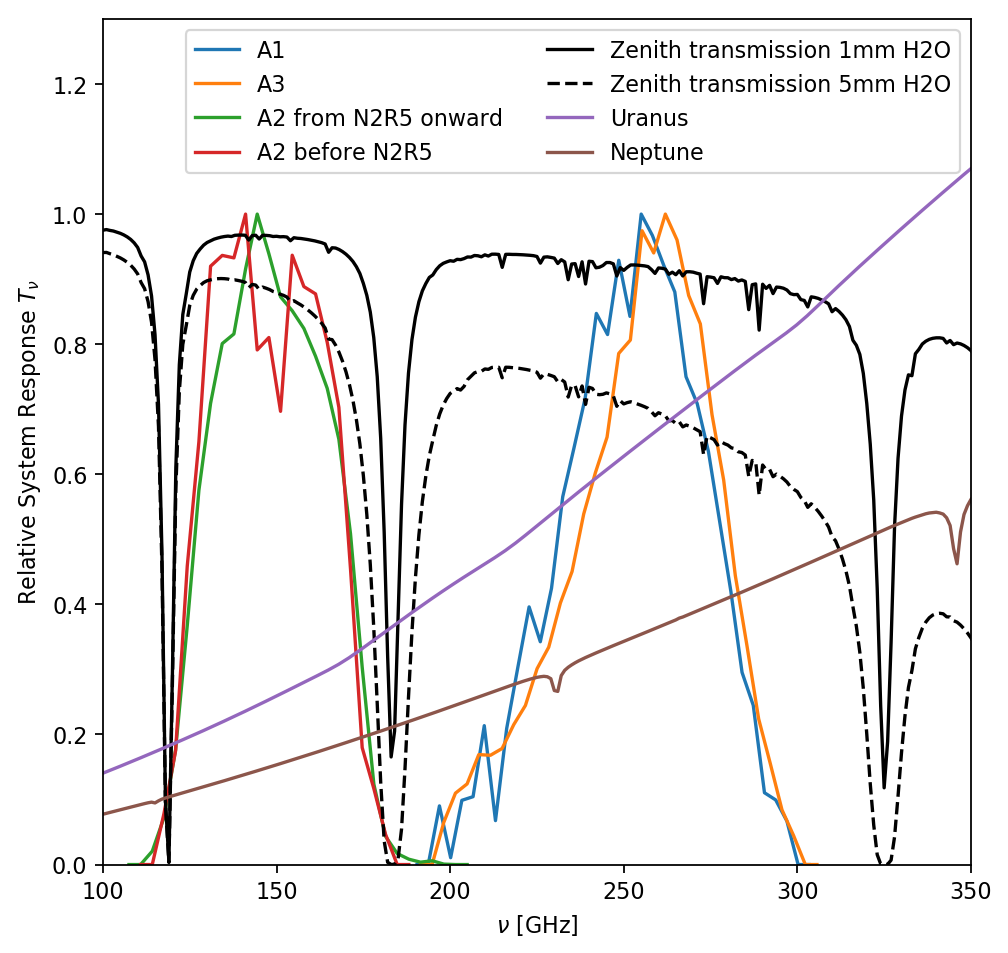
\includegraphics[width=0.75\textwidth]{Figures/SpectralBands/bandpasses_nika2.png}
\caption[NIKA2 transmission]{Relative system response of the three NIKA2 arrays as a
  function of frequency. For illustration we also plot atmospheric transmission obtained with the ATM model 
 \cite{ATM} for different values of precipitable water vapor. The spectra of ESA4 model of Uranus and ESA5 model of Neptune \cite{ESAmodel} in the frequency range are overplotted with arbitrary normalization.} 
 \label{spectralband1}
\end{center}
\end{figure}

 

The NIKA2 spectral bands were measured in the laboratory using a
Martin-Puplett interferometer built in-house \cite{durand}.  Both
arrays and filter bands were considered in the measurements. These
were obtained from the difference of two black bodies, hence they
include a $\nu^2$ Rayleigh-Jeans (RJ) spectral term.
Figure~\ref{spectralband1} shows the relative spectral response for
the three arrays (corrected of the RJ term).  Notice that array A2 was
replaced by a new one in N2R5 and that the spectral transmissions are
not the same (green and red lines in the figure).

The two arrays operating at 260 GHz, mapping different polarisations,
exhibit a slightly different spectral behaviour probably as can be
seen on figure \ref{spectralband1}. This may be explained by a tiny
difference in the silicon wafer and/or Aluminium film thicknesses. For
instance, the observed shift of the peak frequency, 265 GHz for the V
(A1) array versus 258 GHz for the H one (A3), can be explained by
about 5 microns change in the substrate thickness. Hereafter, the peak
frequencies are referred to as reference frequencies (150 and 260 GHz)
to which correspond the reference wavelengths (2.0 and 1.15 mm), see
tab.~\ref{tab:nika2summary}.


\begin{table}[th]
\begin{center}
\begin{tabular}{|l|l|r|r|r|r|r|r|}
\hline 
\multirow{3}{*}{Water vapor} & \multirow{3}{*}{Elevation} & \multicolumn{2}{|c|}{1 mm (H)} & \multicolumn{2}{|c|}{1 mm (V)} &
\multicolumn{2}{|c|}{2 mm} \\
 & & $\nu_eff$ & $\Delta \nu$  & $\nu_eff$ & $\Delta \nu$  & $\nu_eff$ & $\Delta \nu$ \\
 & & (GHz) & (GHz)  & (GHz)  & (GHz)   & (GHz)  & (GHz)  \\
\hline
\multicolumn{2}{|c|}{No atmosphere} & 254.71 & 49.21 & 257.39 & 48.05 & 150.93 & 40.72 \\
\hline
\multirow{4}{*}{1 mm $\rm H_2O$ $\rightarrow \tau_{225}=$0.067} & 90 deg &  254.46 & 48.72 & 257.12 & 47.95 & 150.93 & 39.71 \\
 & 60 deg & 254.42 & 48.68 & 257.08 & 47.93 & 150.92 & 39.60 \\
 & 40 deg & 254.33 & 48.57 & 256.98 & 47.89 & 150.88 & 39.32 \\
 & 20 deg & 254.00 & 48.21 & 256.62 & 47.77 & 150.75 & 38.45 \\
\hline
\multirow{4}{*}{2 mm $\rm H_2O$ $\rightarrow \tau_{225}=$0.120} & 90 deg &  254.26 & 48.74 & 256.91 & 48.06 & 150.64 & 39.34 \\
 & 60 deg & 254.20 & 48.70 & 256.84 & 48.07 & 150.60 & 39.19 \\
 & 40 deg & 254.02 & 48.60 & 256.65 & 48.08 & 150.48 & 38.80 \\
 & 20 deg & 253.43 & 48.30 & 256.01 & 47.93 & 150.13 & 37.62 \\
\hline
\multirow{4}{*}{3 mm $\rm H_2O$ $\rightarrow \tau_{225}=$0.173} & 90 deg &  254.06 & 48.76 & 256.70 & 48.19 & 150.39 & 39.03 \\
 & 60 deg & 253.97 & 48.73 & 256.60 & 48.21 & 150.32 & 38.84 \\
 & 40 deg & 253.71 & 48.65 & 256.33 & 48.28 & 150.14 & 38.35 \\
 & 20 deg & 252.86 & 48.41 & 255.40 & 47.86 & 149.60 & 36.94 \\
\hline
\multirow{4}{*}{5 mm $\rm H_2O$ $\rightarrow \tau_{225}=$0.278} & 90 deg &  253.67 & 48.82 & 256.28 & 48.45 & 149.96 & 38.47 \\
 & 60 deg & 253.51 & 48.81 & 256.11 & 48.44 & 149.84 & 38.22 \\
 & 40 deg & 253.10 & 48.77 & 255.68 & 48.26 & 149.54 & 37.58 \\
 & 20 deg & 251.74 & 48.67 & 254.20 & 47.75 & 148.68 & 35.82 \\
\hline
\multirow{4}{*}{8 mm $\rm H_2O$ $\rightarrow \tau_{225}=$0.437} & 90 deg &  253.08 & 48.94 & 255.66 & 48.42 & 149.38 & 37.76 \\
 & 60 deg & 252.84 & 48.93 & 255.39 & 48.35 & 149.20 & 37.42 \\
 & 40 deg & 252.21 & 48.94 & 254.71 & 48.16 & 148.77 & 36.64 \\
 & 20 deg & 250.12 & 49.38 & 252.43 & 47.91 & 147.52 & 34.57 \\
\hline
\multirow{4}{*}{10 mm $\rm H_2O$ $\rightarrow \tau_{225}=$0.542} & 90 deg &  252.70 & 49.00 & 255.24 & 48.38 & 149.04 & 37.34 \\
 & 60 deg & 252.39 & 49.01 & 254.92 & 48.29 & 148.82 & 36.97 \\
 & 40 deg & 251.62 & 49.11 & 254.08 & 48.13 & 148.31 & 36.12 \\
 & 20 deg & 249.07 & 49.75 & 251.28 & 48.24 & 146.85 & 33.93 \\
\hline
\end{tabular}
\caption[Effective frequencies and bandwidthes]{Effective frequencies (for Uranus) and bandwidth of the NIKA2 bands for
  various atmospheric conditions and elevation.}
\label{tab:bandwidths}
\end{center}
\end{table}

%What actually matters more than the ``central frequency'' that depends on many
%assumptions and definitions are the bandpasses. We should make available in a
%.fits file, clearly, our bandpasses to avoid future misunderstanding and propagation of
%false numbers. Official values should be 150 and 260~GHz. We should also clearly
%state that these measured bandpasses were done with the difference of two
%black-bodies, hence they include a $\nu^2$ RJ term.\\

{\color{red} LP: to be moved to Section Calibration ? Opacity ? }


The total system response is the multiplication of the atmospheric
transmission with the relative system response. To derive the
atmospheric transmission, we use GILDAS ATM 2009 model \cite{ATM}, computed for
the IRAM 30-m telescope, with so called {\it midlatwinter} conditions. We select in the model
grid an atmosphere with $T=268.3 \ {\rm K}$ and a pressure of $703.5 \ {\rm hPa}$. The
effective frequency of the passband is defined by:
\begin{equation}
\nu_{eff}( \sec \delta, mm_{H_{2}O}) = \frac{ \int_{0}^{+\infty} S_{\nu}
  T_{\nu}(\sec \delta, mm_{H_{2}O}) \nu d\nu } { \int_{0}^{+\infty} S_{\nu} T_{\nu} d\nu}
\label{eq:nueff0}
\end{equation}

{\color{blue} FXD: we should integrate over SOmega (nu-2). For
  MartinPuplett measurements, the source spectrum was RJ (nu2) so that
  cancels out to find Tnu. Snu is for an extended source. Deltanu
  should be with respect to a spectrum, for example RJ. I think the
  table 2.1 is not very useful. It could be a figure (nueff as a
  function of tauLOS (elevation is not relevant)? or just few numbers:
  we should at the end state what is nueff and deltanu for average
  conditions. Nomenclature: 1mm(H) is not the usual denomination... }


where $T_{\nu}$ is the total system response, normalized between
0. and 1. (i.e. a relative response as a function of the frequency),
hereafter referred to as RSR (Relative System Response), $S_{\nu}$ is
the source spectrum. Table~\ref{tab:bandwidths} lists this effective frequency,
computed for Uranus spectrum (ESA4 model, \cite{ESAmodel}), for different atmospheric
water vapor contents and different elevations. 
Table~\ref{tab:bandwidths} also list the bandwidth, defined as:
\begin{equation}
\Delta\nu = \int_{0}^{+\infty} \frac{T_{\nu}}{Max(T_{\nu})}
d\nu
\end{equation}
where the $Max(T_{\nu})$ ensure the RSR span the whole 0.0 to 1.0 range.

From Table~\ref{tab:bandwidths}, we see that the 2 mm band is somewhat
sensitive to the atmospheric conditions, especially at low
elevation. Note that these effective frequencies are {\em not} the
reference frequencies for the band, respectively 150 GHz and 260 GHz
for the A2 and A1, A3 arrays. These reference frequencies are chosen
as round numbers in the middle of the bands to define NIKA2
photometric system as will be discussed in section~\ref{se:cal_HA}.

%
% LP: the paragraph below rather belongs to the Opacity section
%
%Using the NIKA2 bandpasses for N2R9, we can integrate the ATM
%atmospheric model to compute the expected ratio between the
%atmospheric opacity of the two NIKA2 channels. 
%Figure~\ref{thopacities} shows the atmospheric opacity
%ratio of the 2 and 1 mm channels as a function of the opacity for the
%1 mm one.

%\begin{figure}[ht] % Inline image example
%\begin{center}
%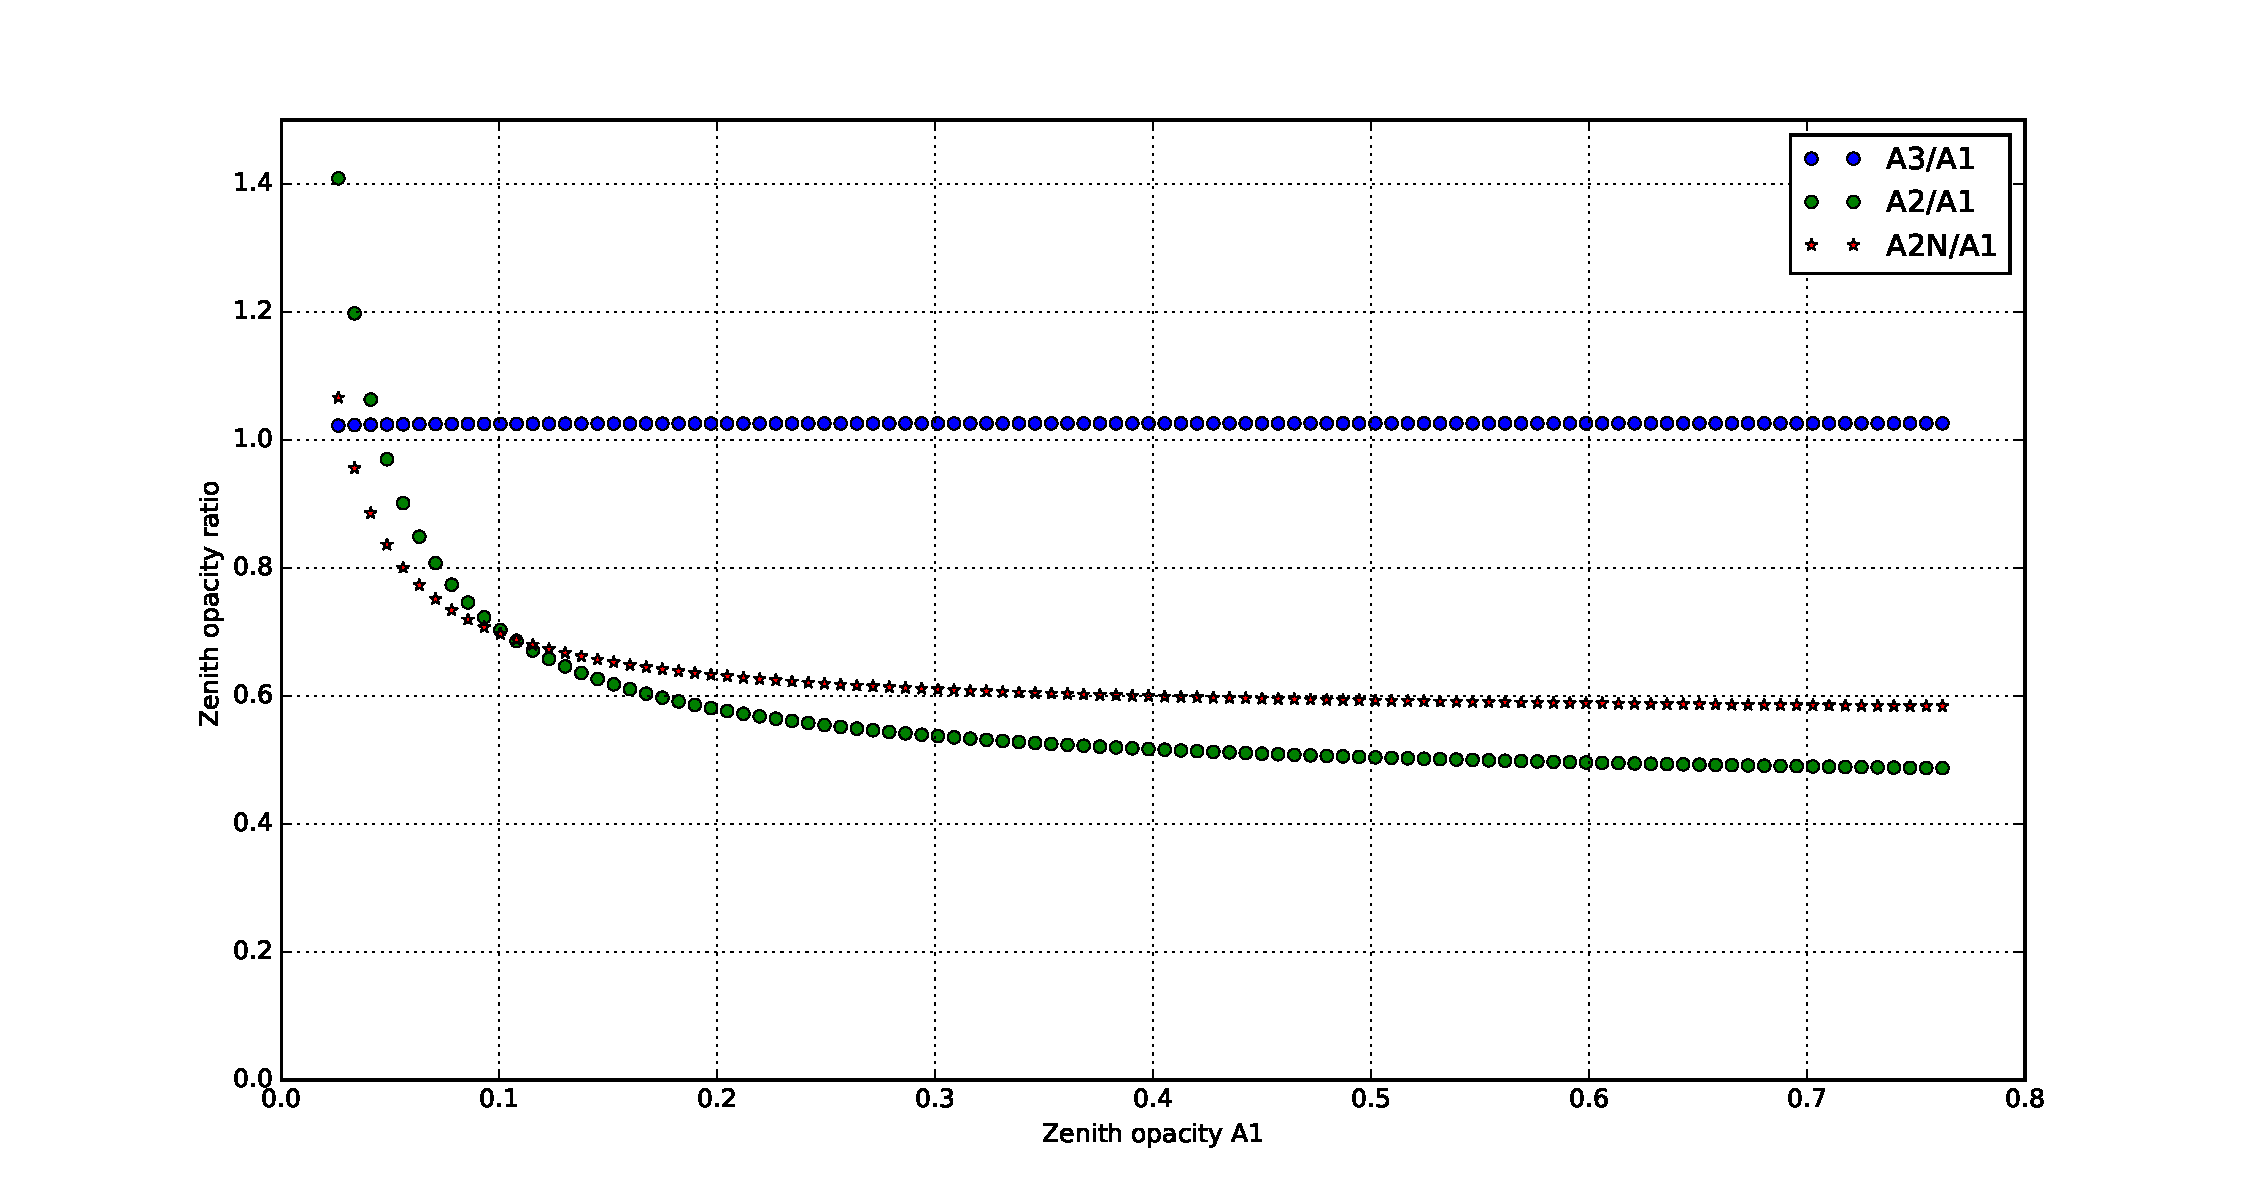
\includegraphics[width=\textwidth]{Figures/SpectralBands/opacity_ratio_vs_tau1.pdf}
%\caption{Expected atmospheric opacity ratio of the 2 and 1 mm channels as function 
%of the opacity at 1 mm. {\bf FM: what is A2N/A1 ?} {\bf FM: why is A3/A1=1 ?}}
%\label{thopacities}
%\end{center}
%\end{figure}





%-------------------------

\subsection{Cryogenics}

The optimal operation of the detectors is achieved at a temperature of around
150\,mK, well below the Aluminium superconducting transition. For this reason,
NIKA2 employs a custom dilution fridge to cool down the focal plane, and the
refractive portion of the optics, for a total mass around 100 kg, deeply in the
sub-Kelvin regime. Despite the complexity and size of the system, the operation
of NIKA2 does not require external cryogenic liquids and is fully remotely
controllable.

\subsection{KIDs and electronics}
\label{se:array}

The 150\,GHz channel is equipped with A2 that is an array of
616\,pixels, arranged to cover a 78\,mm diameter circle. Each pixel has a size of
$2.8\times2.8\textrm{\,mm}^2$. The array A2 is connected over four different
readout lines. In the case of the 260\,GHz band detectors, the pixel size is
$2\times 2\mathrm{\,mm}^2$, to ensure a comparable sampling of the focal
plane. In order to fill the two 260\,GHz arrays A1 and A3, a total of 1,140 pixels are
needed in each of them. The focal planes are all based on thin Aluminium films
deposited by e-beam evaporation under ultra-high vacuum conditions over a
Silicon substrate.

The key advantage of the KID technology is the simplicity of the cold
electronics and the multiplexing scheme. In NIKA2, each block of around 150
detectors is connected to single coaxial line providing the excitation and the
readout at the two ends. Each of the readout lines is linked to the input of a
cryogenic (4 K) low-noise amplifier. The warm electronics required to digitize
and process the pixels signals is composed of twenty custom readout cards (one
per feed-line).

%In this document, the 2\,mm array is called A2, while the two 1\,mm arrays are
%called A1 and A3.


\subsection{KID photometry and tuning}

\begin{figure}[!b]
\begin{center}
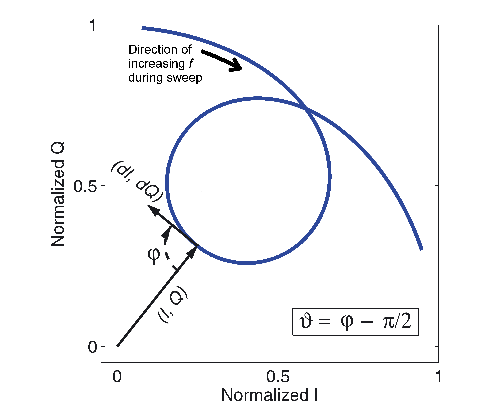
\includegraphics[width = 0.7\textwidth]{Figures/resoCircle-eps-converted-to.pdf}
\caption[KID resonance circle]{Sample resonance circle in the IQ plane. Both the
  tuning procedures are based on the measurement of the angle $\vartheta$
  between the two vectors ($I, Q$) and ($dI, dQ$)}
\label{figResoCircle}
\end{center}
\end{figure}

Kinetic Inductance Detectors are superconducting resonators whose resonance
frequency shifts linearly depending on the incoming optical power. The measure of such
frequency shift $\Delta f$ is what allows us to use KID as mm-wave detectors.

For the KID readout, an excitation signal is sent into the cryostat on the
feedline coupled to the KID. The transmitted signal can be described by its
amplitude and phase, or, as is common practice for KID, by its components that
are In-phase ($I$) and in Quadrature $Q$ with respect to the excitation
signal. When a frequency sweep is carried around a KID resonance, the
transmitted signal makes a sort of circle in the $I-Q$ plane, as shown
in Fig.~\ref{figResoCircle}.
The goal is now to relate the variations $(\Delta I, \Delta
Q)$ along this circle induced by incident light to the $\Delta f$. For this, the
electronics modulates the excitation frequency at about 1\,kHz with a known
$\delta f$ frequency variation and the read out gives the induced $(dI,
dQ)$. Projecting linearly $(\Delta I, \Delta Q)$ on $(dI, dQ)$ therefore
provides $\Delta f$. This value, in Hz, is the raw input timeline to the
pipeline and will be futher calibrated into astronomical units
(sect.~\ref{se:calibration}). For historical reasons, this way of deriving KID
signals has been nicknamed \emph{RfdIdQ}. More details on this process are given
in \cite{Calvo13}.\\

Not only incident astronomical light reaches the KIDs and contributes to Cooper
pair breaking. Any change in the background optical load (due, for example, to changes in
the atmospheric transmission or in the elevation) contributes as well to the
shift of the resonances. In order to maximize the sensitivity of a KID, the
excitation signal used to read it out must always be near its resonance
frequency. We therefore have developped a tuning algorithm that takes care of
this optimization. Tunings are performed during the first subscan of each
observation in order to be optimally tuned at the same elevation and sky
conditions as the source. It takes only a few seconds when the $f_{tones}$ are
close to the current functionning point. In order to always be in these
conditions, continuous tunings are done between two scans when NIKA2 is not observing.

A specific case is when we do {\tt skydips}. In this case, we tune all the KIDS
at the beginning of each subscan/elevation step on purpose to monitor the
induced variation of $f_{tone}$ by the sky load.



%----------------------------------------------------------------------------------------
%	3./ Observing mode
%----------------------------------------------------------------------------------------
\section{Observations}
\label{se:observations}

%----------------------------------------------------------------------------------------
%	3./ Observing mode
%----------------------------------------------------------------------------------------
%\section{Observations}
%\label{se:observations}

This section presents the different observation modes that are used at
the \trentemetre\ IRAM telescope for both commissioning and
scientific-purpose observations with NIKA2. {\lp Each observation
campaign is organized as observing pool allowing to optimize
observations of several science targets in a flexible way.}
Most of the used observing scans are based on on-the-fly raster scans,
which consists of several linear scanning legs, combined to one
map. Their characteristics have been tailored for NIKA2 performance.
%Some of them are common
%to usual IRAM observing modes (\emph{e.g.}~''on the fly'' raster scans), some of them
%have been designed specifically for \nika\ (e.g.~the focus sequence).
% \todo{define PAKO}

%\subsection{Overview of different types of scans}

%Once the KIDs are tuned and \nika\ is ready for observations, before actually
%observing a scientific target, one needs to adjust the focus and pointing of the
%telescope. In the case of EMIR typically, these two parameters are adjusted iteratively by
%alterning ``pointing'' (\aka\ ``cross'') and ``focus'' scans to optimize the
%centering of a bright point source on a reference detector and to maximize the
%incoming flux on it. With \nika\ , mostly due to absence of horns, this
%procedure is not optimal. Indeed, it was noticed that the position of the source
%moved by several arcsec with the displacement of M2
%during the focus procedure and this would alter the flux
%measurement on a fixed reference position too much to enable focus
%optimization.

%\begin{figure*}[!thbp]
%\begin{center}
%  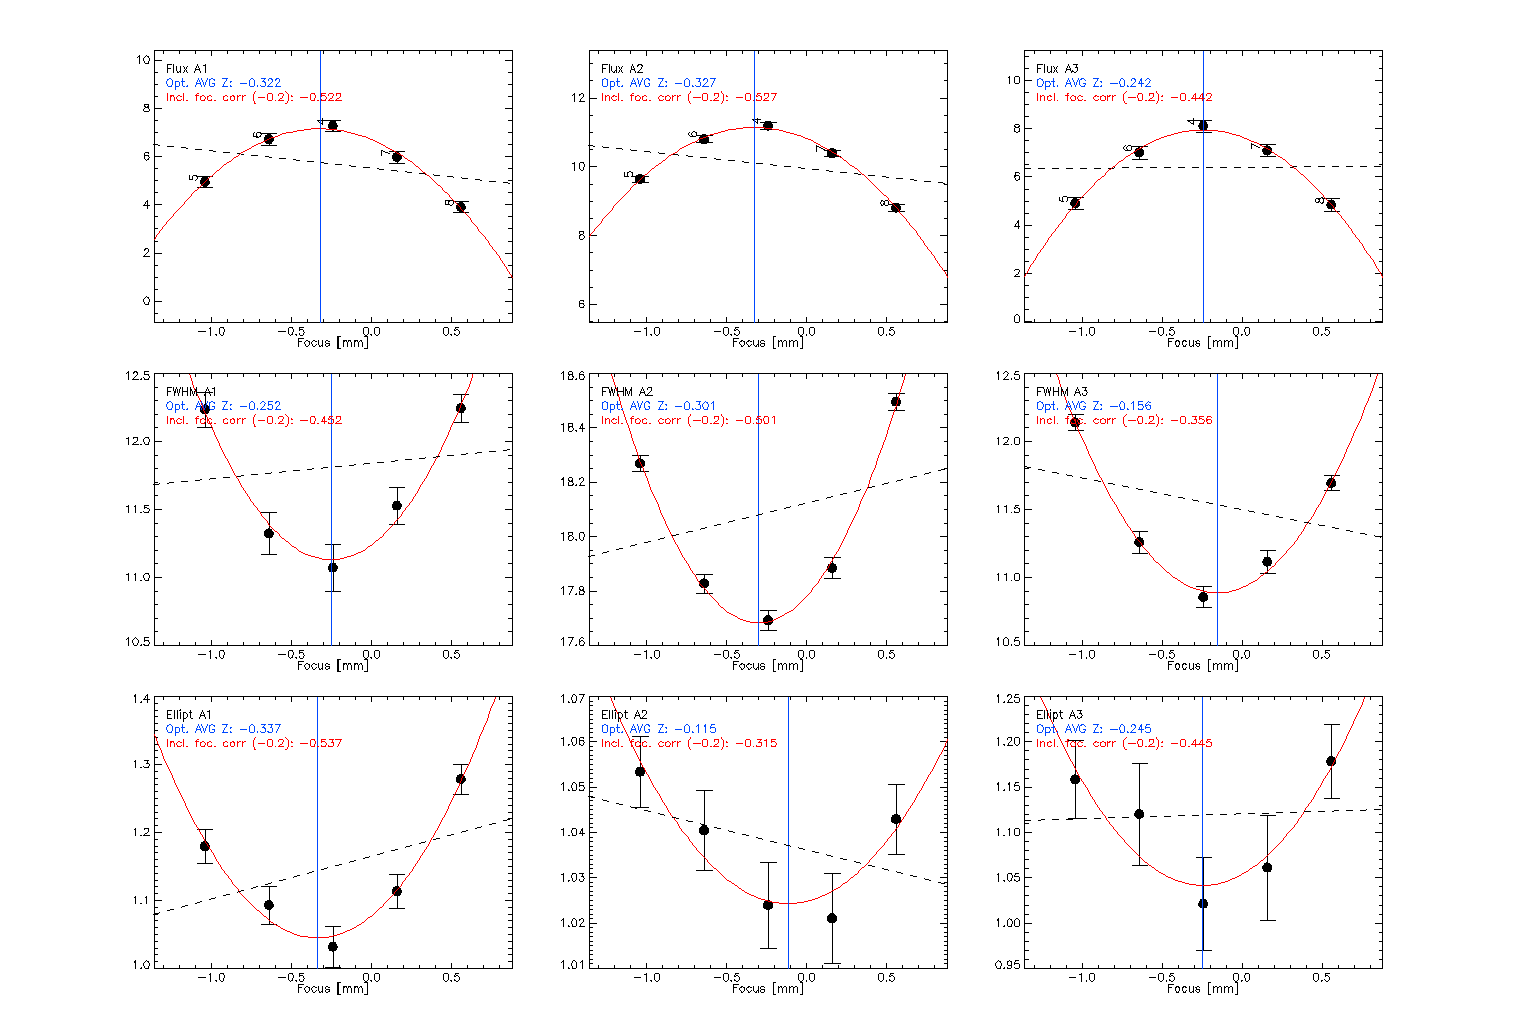
\includegraphics[clip, angle=0, trim={3cm, 12cm, 3cm, 1.5cm}, width=0.75\textwidth]{Figures/plot_20180120s8_zfocus.png}
%\caption[]{Example of axial focus measurement using a dedicated focus
%  observation sequence of the bright quasar 3C84 during the Juanuary
%  2018 campaign (N2R14) in good observing conditions. Flux (first
%  row) and FWHM (second row) measurements are
%  shown as a function of the axial focus offsets for Array 1 (first
%  column), Array 2 (second column) and Array 3 (third column). The
%  best-fitting parabola is shown in red. To help the observer
%  assessing the parabolic fit quality, the best-fit linear model is also drawn
%  with dashed black lines. 
%  The blue vertical line locates the best-fitting $z$-focus value of
%  each fit. The optimal focus values derived from flux
%  maximization and FWHM minimization agree to better than 0.1\,mm in these
%  conditions of observation. %While ellipticity may be often regarded as a confirmation
%  %more than a decisive criterion (due to larger uncertainty on its measure), the
%  %associated minimum is also in good agreement with the values derived from flux
%  %and FWHM measurements in this example taken in stable atmospheric
%  %conditions.
%}
%\label{fig:focus-example}
%\end{center}
%\end{figure*}

\subsection{Focus}
\label{se:axial_focus}

Observation pools start with setting the telescope focus since NIKA2 large
FOV alleviates the need to adjust the pointing beforehand.  
We have designed a specific focus procedure that takes
advantage of the dense sampling of the FOV allowing to map a source
in a short integration time. We perform a series of five successive one-minute
raster scans of a bright (above a few Jy) point source at five
axial offsets of the secondary mirror (M2) along the optical
axis. As the scan size is $1'\times 5'$, the main contribution to each
map mainly comes from the KIDs located in the central part of the FOV.%, typically
%$\{-0.8, -0.4, 0, 0.4, 0.8\}$\,mm w.r.t.~the current $z$-focus (which
%is usually the previous optimal $z$-focus value).
%We then analyse each map to optimize the $z$ position of M2.

%More details are given in
%Sect.~\ref{se:axial_focus}.
%Once the focus is correctly determined, the pointing
%corrections are derived from an EMIR like pointing calibration scan
%(Sect.~\ref{se:pointing}). The instrument is then ready to observe scientific
%targets.

%\subsection{Axial focus}
%\label{se:axial_focus}

%The best axial focus in the central region of the arrays is estimated
%using the
%so-called {\tt focus$\_$OTF} PAKO script, which produces a series of
%five $1'\times 5'$ OTF scans at various values of the focus in $0.4~\rm{mm}$ steps
%around an \emph{a priori} value $z_0$, namely
%$z \in \{-0.8, -0.4, 0, 0.4, 0.8\} + z_0$.
Elliptical Gaussian fits on the five maps provide estimates of
the flux and FWHM along minor and major axes for each focus. 
The best axial focus in the central part of the array is then
estimated as the maximum of the flux or the minimum of the FWHM using
parabolic fits of the five measurements.
%Parabolic fits are
%then used to determine the best focus.%, as illustrated in Fig.~\ref{fig:focus-example}.
%We consider three estimates: i) $\hat
%z_{\rm{peak}}$ the focus that maximizes the estimated flux, which is the
%amplitude of the 2D Gaussian, ii) $\hat z_{\rm{fwhm}}$ the focus that minimizes
%the geometrical FWHM, defined as the quadratic mean of $\rm{FWHM}_{\rm{major}}$
%and $\rm{FWHM}_{\rm{minor}}$, and iii) $\hat z_{\rm{ellipt}}$ the focus that
%minimizes the beam ellipticity, defined as
%$\rm{FWHM}_{\rm{major}}/\rm{FWHM}_{\rm{minor}}$. Fig.~\ref{fig:focus-example}
%shows an example of such a sequence. When deciding on the focus to apply, we
%give priority to the optimal flux, taking an average between values on A1 and
%A3: there is little difference between the two and the 2\,mm channel is
%less sensitive to the focus change than the 1\,mm.

As presented in more details in Sect.~\ref{sec:focus_surfaces}, the focus
surface, that is defined as the locations of the best focus across the whole FOV
is not strictly flat but rather bowl-shaped.
%The way sources are scanned in
%this {\tt focus\_OTF} sequence is designed to save time but it gives more weight
%to the central KIDs.
%Hence, the optimal focus derived from the fits is biased.
To account for the curvature of the focus surfaces and optimize the
average focus across the FOV, we add -0.2\,mm to the best axial focus
in the central part of the array, as derived in the previous
paragraph. This focus offset is measured on data using
a dedicated sequence of de-focused scans, as discussed in
Appendix~\ref{sec:focus_surfaces}. It is in agreement with expectations
derived with optical simulation using ZEMAX\footnote{Web site: \tt{www.zemax.com}}. 

{\lp Axial focus offsets are measured every other hours during daytime and
are systematically checked after sunrises and sunsets, while one or
two checks suffice during the nights. 
Lateral focus offsets can also be checked in a similar way, but are
found to stay constant over periods of time that cover several
observing campaigns.}


%\subsection{Lateral focus}
%\label{sec:focus_X_Y}

%Like in the $z$ (optical axis) direction, it is possible to control the position
%of M2 along the $x$ and $y$ directions. We have tried to determine if there was
%an optimal position in the $(x,y)$ plane that would improve further measurements
%with \nika. We have applied the same procedure as the one described in
%Sect~\ref{se:axial_focus}, this time varying the position of M2 along $x$ or $y$
%rather than along $z$. Examples of such observations are presented on
%Figs.~\ref{fig:X_focus} and \ref{fig:Y_focus}. While the forced parabola fit
%guides the eye towards optimization, one should note the size of the error bars
%and the relatively low variations compared to M2 displacements along the $z$
%axis. This is expected from optical simulations and experience on
%EMIR. Figs.~\ref{fig:X_focus} and \ref{fig:Y_focus} also show as complement,
%images of the residuals of the intensity maps at each M2 position after the
%subtraction of an elliptical gaussian fitted only on a disk of 6 and 15\,arcsec
%(1 and 2\,mm resp.) around the maximum location and outside a ring of 100\,arcsec
%away from the maximum (to fix the background while not being affected by the
%side lobes). These maps of residuals are meant to help to decide on a minimization
%criterion and $x$ or $y$-focus value.

%While we have performed ``many'' of such observations and explored the entire
%parameter space of the $(x,y,z)$~triplet position in a reasonable range of
%several millimeters around a fixed position, it has not been possible to
%demonstrate that any $(x,y)$ positions would improve significantly the
%focusing of the whole system compared to the nominal $(0,0)$ reference
%position. \vu{This confirms the experience of the IRAM staff with EMIR and
%HERA who only act on this $(x,y)$ position about once a year after
%specific, dedicated and delicate measures. This effort is necessary
%to find an optimum lateral focus position which is stable with
%elevation. For \nika\, the adopted strategy has been not to change the
%lateral focus parameters and only rely on $z$-focus optimization for
%observations. However, lateral focus measurements with NIKA2 have to be
%scheduled in the future.} 

%\begin{figure*}[h!]
%\centering
%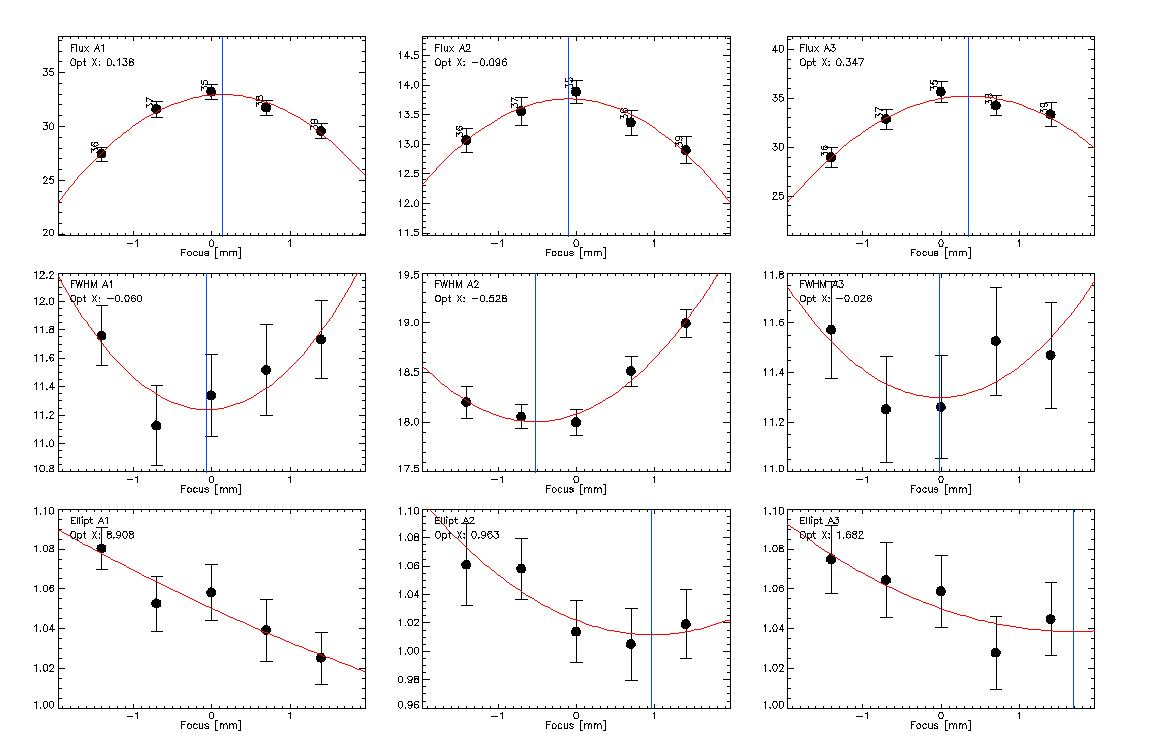
\includegraphics[height=8cm]{Figures/plot_20170223s39.png}
%\hspace{0.5cm}
%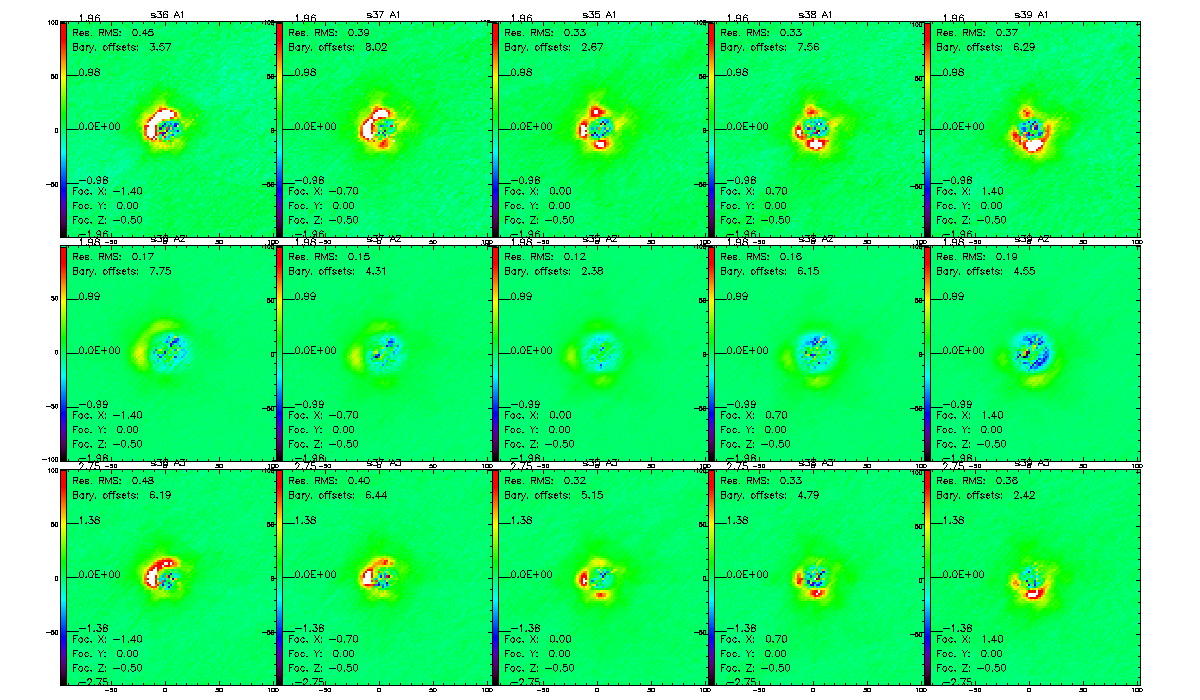
\includegraphics[height=8cm]{Figures/residuals_focus_otf_20170223s39.png}
%\caption[Lateral X focus measurements]{\emph{top panel: }X-focus measurement using a
%    parabolic fit of the flux, beam FWHM and ellipticity on a sequence
%    of five OTF scans on Uranus (20170223s39-43) \emph{bottom panel: }Beam residuals
%    after subtracting a model of the main beam for each OTF-scan of the X-focus
%    session. (N2R9)}
%\label{fig:X_focus}
%\end{figure*}

%\begin{figure*}[h!]
%\centering
%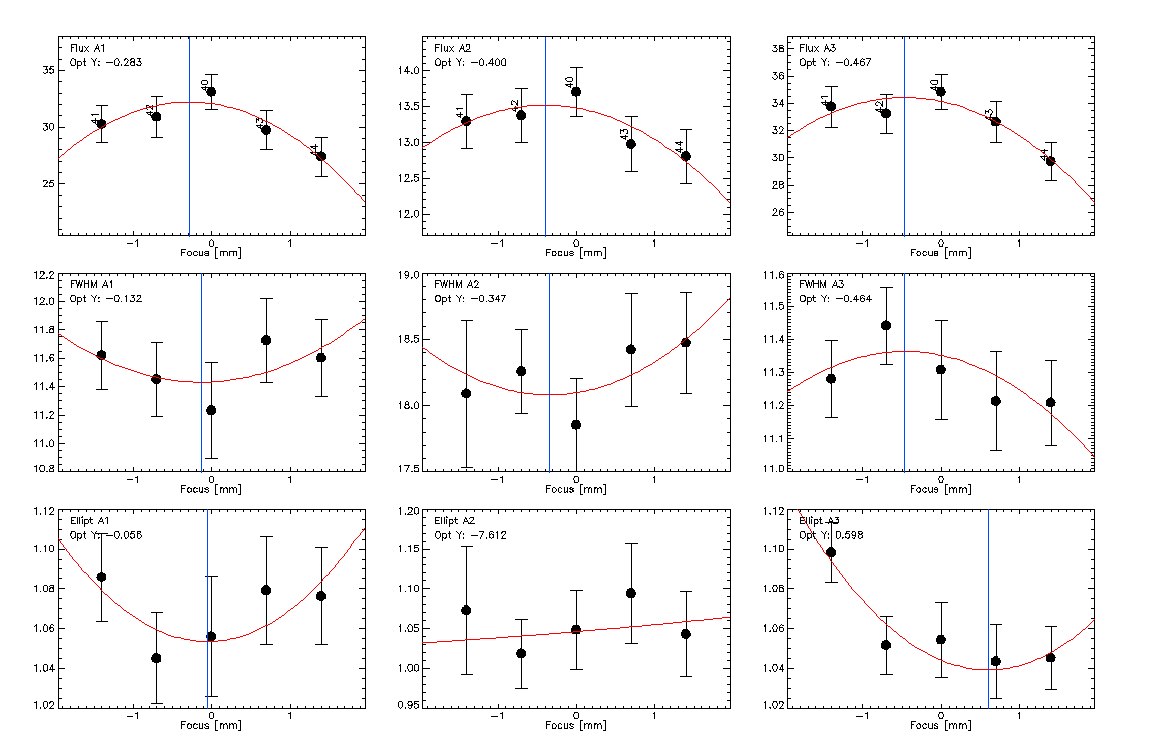
\includegraphics[height=8cm]{Figures/plot_20170223s44.png}
%\hspace{0.5cm}
%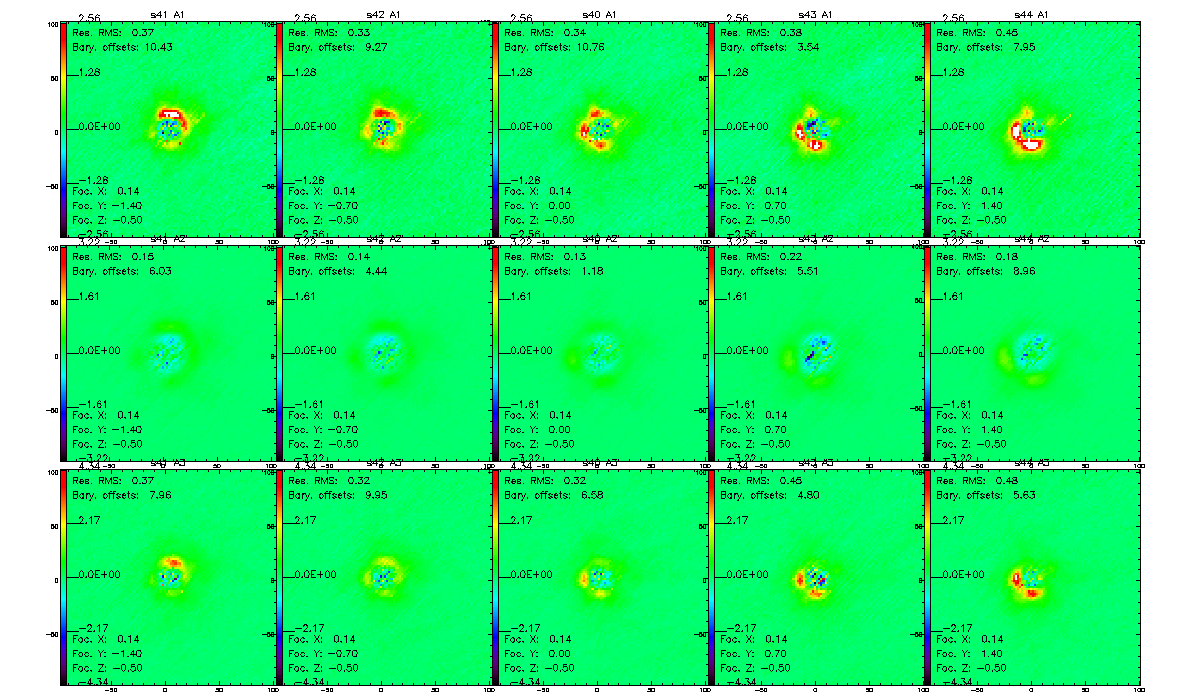
\includegraphics[height=8cm]{Figures/residuals_focus_otf_20170223s44.png}
%\caption[Lateral Y focus measures]{\emph{top panel: }Y-focus measurement using a
%    parabolic fit of the flux, beam FWHM and ellipticity on a sequence
%    of OTF scans on Uranus (20170223s44-48). \emph{bottom panel: }Beam residuals
%    after subtracting a model of the main beam for each OTF-scan of the Y-focus
%    session. (N2R9)}
%\label{fig:Y_focus}
%\end{figure*}


\subsection{Pointing}
\label{se:pointing}
% + RTA pointing estimate method
% + pointing model
% + pointing error (scan-to-scan scattering)

Once the instrument is correctly focused, we can estimate pointing corrections
before scientific observations.
%Even though EMIR only has a single pixel on the sky, the pointing procedure
%used for NIKA2 is very similar and is described in the next subsections.
%
%\paragraph{Pointing monitoring}
%
%\begin{figure}[ht!]
%\begin{center}
%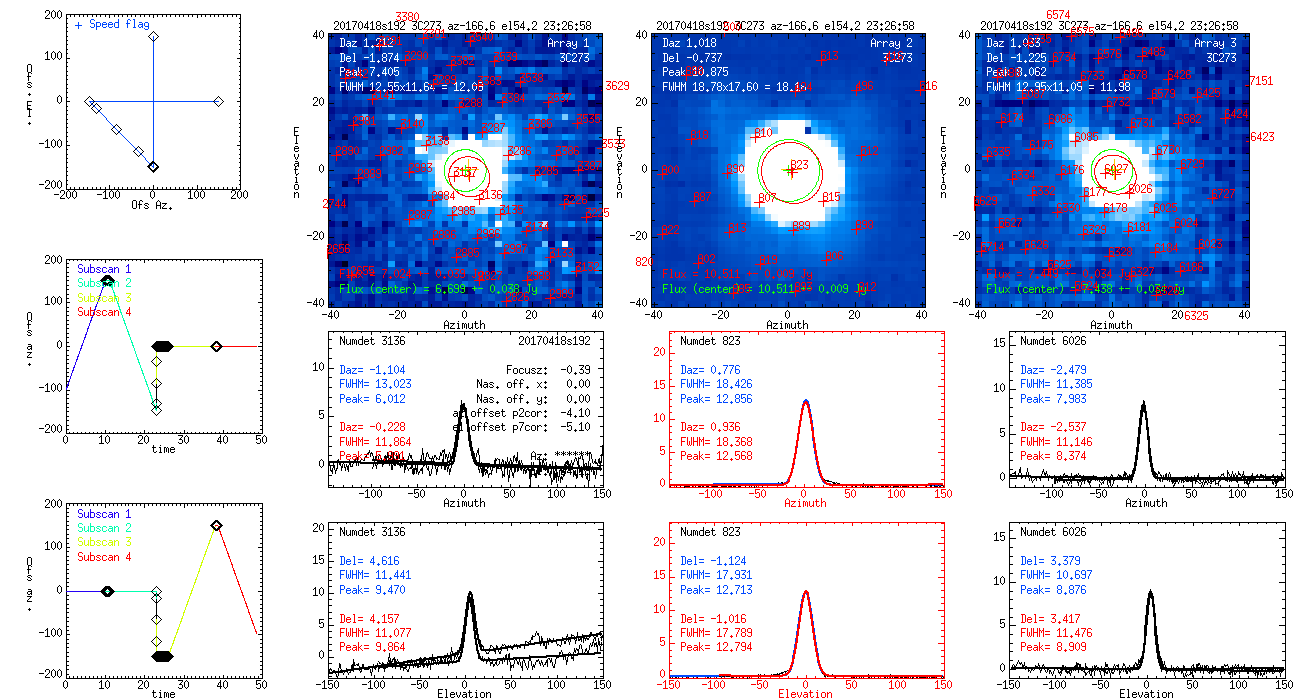
\includegraphics[clip, angle=0, scale = 0.30]{Figures/plot_20170418s192.png}
%\caption[Summary plots of the reduction of pointing scan.]{Top plots
%  show the combined map for array 1, 2 and 3, which enable a check of
%  the overall quality of the scan, while bottom plots show the set of azimuth
%  and elevation profiles for one reference detector per array. The
%  reference detector per array is highlighed with a red cross in the
%  centre of the map. The pointing reference detector of
%  \nika\ is the 2\,mm reference detector, the azimuth
%  and elevation profiles of which are shown in the central bottom
%  plot. The location of the peak in azimuth and elevation, as observed by the
%  reference detector gives the pointing offsets of the current scan.
%}
%\label{fig:ptg}
%\end{center}
%\end{figure}
%
%\begin{figure}[ht!]
%\begin{center}
%\includegraphics[clip, angle=0, trim={0, 0, 3cm, 0}, width=0.65\textwidth]{Figures/pointing_stats_N2R9.eps}
%\caption[Pointing session results]{Pointing offsets during Run9 observations,
%  before (blue to green) and after (yellow to red) the
%  derivation of Nasmyth offsets with a pointing session on Feb.~26th, 2017.}
%\label{fig:pointing_stats_n2r9}
%\end{center}
%\end{figure}
%
Based on general operating experience at the \trentemetre\ telescope, we use the so-called
{\tt pointing} or {\tt cross-type} scans to monitor the pointing during observations. The
telescope executes a back and forth scan in azimuth and a back and forth scan in
elevation, centered on the observed source. We fit Gaussian profiles
from the timelines of the reference detector, which is chosen as a
valid detector located close to the center of Array 2. We use the
estimated position of the reference detector to derive the current pointing
offsets of the system in azimuth and elevation. This correction is
propagated to the following scans.
%These offsets can then
%be used to make the optical axis of the telescope to coincide with the
%optical axis of NIKA2 and thus optimize the pointing of the following scan.
%These offsets can then be passed
%to PAKO to make the optical axis of the telescope
%to coincide with the optical axis of NIKA2 and thus recenter the next scan.

%\paragraph{Pointing session}
%\label{se:pointing_session}

%Such scans and their analyses are also used to improve the pointing model of
%\nika. A pointing session consists in observing about 30 sources on a wide range
%of elevations \new{and azimuth angles} while monitoring the pointing offsets
%that are measured for each observation. These offsets are then passed to the
%IRAM staff who finds the pointing model parameters that minimize and symmetrize
%the scattering of these offsets. Based on these results, the Nasmyth offsets
%parameters that enter the IRAM pointing model are
%adjusted. Fig.~\ref{fig:pointing_stats_n2r9} shows the pointing corrections that
%had to be applied during Run9, before and after the modification of the Nasmyth
%offsets. The dispersion of the offsets is the figure of merit of the pointing
%corrections. Their distribution after the corrections (in yellow to red) is
%clearly more symmetric and narrower than before. During N2R9 run, the rms of
%the residual scatter after the correction was 1.62\,arcsec rms in
%azimuth and 1.37\,arcsec rms in elevation.


\subsection{Skydip}
\label{se:skydip}

A {\tt skydip} scan with NIKA2 consists in a step-by-step span
of a large range of elevations. This is used in order to calibrate the
KID responses with respect to the atmospheric background for
atmospheric opacity derivation, as discussed in
Sect.~\ref{se:opacity}.
Whereas with the heterodyne receivers, skydips can be
conducted continuously slewing the telescope in elevation, this
option is not feasible with NIKA2, as the KIDs need to be retuned
for a given airmass.
A NIKA2 skydip comprizes eleven steps in
the elevation range from 19 to 65 degrees, regularly spaced in
airmass. For each step, we acquire about twenty seconds of data
to ensure a precise measurments. KIDs are tuned at the beginning of
each constant elevation sub-scan (hence once per airmass).
%The variation of their resonance
%frequency reads
%
%\begin{equation}
%  f_{\rm{reso}}^k  = C_0^k - C_1^k T_{atm}[1-e^{-\tau/\sin\delta}]
%\label{eq:skydip_1}
%\end{equation}

%An illustration is presented on Fig.~\ref{fig:ftone_vs_elev}. More details on
%the analysis of these {\tt skydip} scans are given in Sect.~\ref{se:opacities}.

%\begin{figure}[ht!]
%\begin{center}
%  \includegraphics[clip, angle=0, scale=0.75]{Figures/skydip_report.eps}
%\caption[skydip]{Variation of the resonance frequency of a KID
%  \new{$f_{\rm{reso}} = \ftone + \delta \ftone$},  as a function of the
%  elevation during a {\tt skydip} scan.}
%\label{fig:ftone_vs_elev}
%\end{center}
%\end{figure}

\subsection{Beam map}
\label{se:beammaps}

A \bm\ scan is an observing procedure to map a bright compact source,
often a planet, with
an elevation step small enough to meet Nyquist sampling of the 1\,mm beam,
namely 4.8''. We observe the source with a raster scan in (az,el)
coordinates of $13\times7.8$~arcmin$^2$, either with the telescope
performing a series of continuous slews at fixed elevation or at fixed azimuth. 
A continuous scanning slew defines a subscan. 
The fixed-elevation scanning has the advantage of nulling the air mass variation
across a subscan, while the fixed-azimuth scanning offers an
orthogonal scan direction to the former:
the combination of both gives a more accurate determination of the far side
lobes.
%The scan size ensures that the entire FOV is observed with good margins
%for beam mapping even on the edges and good margins for baseline derivation and
%subtraction in the scanning direction.
The scan size is optimized to enable maps to be made for all
KIDs, even those located at the edges of the array. Larger size in the scanning
direction allows for correlated noise subtraction.
During subscans, the telescope moves at
65\,arcsec/s. This value results of a tradeoff between the need to scan as
fast as possible to minimize atmospheric contamination and the
necessity to keep subscans no shorter than 10\,s (telescope
constraint). The need to have Nyquist sampling of 11'' beams along the
scan direction translates into a maximum speed of 97\,arcsec/s
for our nominal acquisition rate of 23.8\,Hz and is thus largely met. Subscans
last 12\,s, the entire scan lasts about 25\,min, which is short enough
to minimize the contribution of the atmospheric fluctuations. 
% Alessandro advice: cancel the following part of the sentence: not true in absolute
% (depending on the atmospheric conditions)
%, which is short enough to prevent
%losing the signal due to atmosphere-induced (1/f) background variations that would
%move the resonance away from the tone probing it.

More details on these observations are given in Sect.~\ref{se:geometry}
where we describe how to actually exploit them to derive individual KID
properties.




%----------------------------------------------------------------------------------------
%	4./ Data reduction
%----------------------------------------------------------------------------------------
\section{Data Reduction}
\label{se:dataproc}

%----------------------------------------------------------------------------------------
%	4./ Data reduction
%----------------------------------------------------------------------------------------
%\label{se:dataproc}

The raw KID data ($I$, $Q$, $\Delta I$, $\Delta Q$) and the telescope
source-tracking data are synchronized by the NIKA2 acquisition system using a
clock that gives the absolute astronomical time, that is the telescope
pulses per second, to define the NIKA2 raw data. From the KID raw
data, we compute a quantity that is proportional to the KID
frequency shift using the \emph{RfdIdQ} method, as described in
Sect.~\ref{se:tuning}. This quantity, which is hence proportional to
the input signal, constitutes the KID time-ordered information (TOI).

%For each observing scan, NIKA2 produce a datastream via the data
%acquisition software, which synchronises with the telescope data using
%pulses per second (pps). This clock is itself synchronous to the
%absolute astronomical time. Using the \rf\ photometric
%estimator, as discussed in Sect.~\ref{se:tuning}, we derive the
%timelines of the KID resonance frequency estimate, which is a quantity
%proportionnal to the flux absorbed by a KID and
%homogeneous to Hz~\citep[see]{Calvo2013}. These time ordered
%information (TOI), together with
%the time-stamped pointing information produced by the telescope,
%constitute the raw data.

We have developed a dedicated data reduction pipeline to
produce calibrated sky maps from NIKA2 raw data. This pipeline was first 
developed for the data analysis during the commissioning campaigns and
is currently used for science-purpose data reduction. The calibration
and performance assessment relies on this pipeline. 
A detailed description of this software will be presented in a companion
paper \citep{Ponthieu2019}, as well as an application to blind source
detection. Here we summarize the main steps of the data
reduction. {\lp Moreover, we focus the discussion on the treatment of
point-like or compact sources, which are used for the
performance assessment.}

%\section{Data Reduction}
%\label{se:dataproc}
%
%Because each matrix of \nika\ is a filled array with more than one
%detector per \new{main beam} PSF on average, and because the atmosphere and electronic noise act as
%correlated low frequency parasites, the data reduction of \nika\ does not
%proceed on an individual KID basis in general. This, in addition to the
%necessary pointing information specifies some of the data reduction
%process. In short, the data reduction proceeds as such:
%
%\begin{itemize}
%\item Low level processing (Sect.~\ref{se:ll_proc})
%\item Pointing reconstruction (Sect.~\ref{se:ptg})
%\item TOI calibration and opacity correction (Sect.~\ref{se:flux_calib})
%\item TOI processing (Sect.~\ref{se:toi_proc})
%\item Map projection (Sect.~\ref{se:map_projection})
%\item Photometry (Sect.~\ref{se:intro_photometry})
%\end{itemize}

%\noindent{\emph{Low level processing:}
%\paragraph{Low level processing.}
\subsection{Low level processing}
\label{se:ll_proc}
%A first step of the analysis is to read the data produced by \nika's
%acquisition. The data as such comprise various quantities that describe the
%variations of the KID's resonance frequencies, such as $I$, $Q$, $dI$,
%$dQ$. From these quantities, and throughout this work, we use our so called
%\rf\ photometric estimator that combines them into a quantity that is
%proportionnal to the flux absorbed by a KID \citep[see]{Calvo2013} and
%homogeneous to Hz, as discussed in Sect.~\ref{se:tuning}.
We isolate the relevant fraction of the data for scientific
utilisation and {\lp we mask KIDs that do not meet the selection criteria, as
discussed in Sect.~\ref{se:avg_kidpar},} or
timeline accidents (glitches). Specifically, we flag out cosmic rays,
which impact only one data sample per hit due to the KID fast time
constant~\citep{Catalano2014}, %periods
%dedicated to the KID resonance frequency {\tt tuning}
%(Sect.~\ref{se:tuning}),
%of the KID tones to their resonance frequency
and the KIDs for which the noise level exceed $3\sigma$ of the average
noise level of all other KIDs of the same array.  
%In addition to this, we look for and remove the - rare - cosmic rays
%events. KIDs have such fast time constants that unlike bolometers, these events
%affect a sole sample that is easy to detect by a simple comparison to the rms of
%the TOI a few second window. These affected samples are remplaced by a simple
%linear interpolation of their surrounding (not to leave holes in the TOI) but
%are flagged in order not to project false data on the final map.
%
%We also have a series of tests that read the flags produced by the acquisition
%overall: discontinuity in the temperature within the cryostat as well
%as detector tuning that automatically trigger at the beginning and the
%end of each scans are discarded.  
%potential jumps in the cryostat or acquisition
%monitoring. Most important are the flags related to the tuning. Because the
%acquisition file boundaries are not strictly linked to the beginning and the end of
%a scan, we must discard everything that happens before the last tuning of the
%beginning, and everything after the first automatic tuning that happens when the
%scan is done.
%
%Because the tuning of KIDs might fail from time to time depending on the weather
%conditions for instance, we systematically check each KID and see if its noise
%is far from the average noise of all other KIDs in the same array, with a
%typical $3\,\sigma$ threshold. This criterion may seem a bit tight, but in any case, KIDs
%are inverse noise variance weighted in the final map projection, so they would
%be given relatively low weight anyway (see Sect.~\ref{se:map_projection}).

%\paragraph{Pointing reconstruction.}
\subsection{Pointing reconstruction}
\label{se:ptg}
We produce a timeline of the pointing positions of each KID with
respect to the targeted source position (usually located at the center of the
scan) using two sets of information. First, the control system of the
telescope provides us with the absolute pointing of a reference point
of the focal point, which is coincident with the reference KID after
the pointing correction are applied, as described in
Sect.~\ref{se:pointing}. Second, we estimate the offset positions of
each KID with respect to the reference KID using a dedicated
procedure that is referred to as the focal plane reconstruction, as
presented in Sect.~\ref{se:geometry}. After this step, we are able to
distinguish KIDs that are on-source from those that are off-source,
which is a key information for dealing with the correlated noise. 
%This step consists in addressing each sample of each KID to the correct sky
%coordinates and their associated map pixel. The pointing data, as
%produced by the control system of the telescope, \aka\ NCS, are passed to the
%\nika\ raw data. They describe the absolute pointing of a reference
%point in the focal plane in various quantities, the
%absolute azimuth and elevation $(\alpha,\delta)$ of the source, together with
%offsets $(\Delta\alpha_t, \Delta\delta_t)$ \wrt~these. Because our final maps
%will be centered on a fixed position (typically the center of the source that is
%aimed by the focal plane reference position), we are especially interested in
%pointing offsets \wrt~this position. We therefore detail here the
%derivation of these offsets.
%
%We store KID pointing offsets \wrt\ the reference position in Nasmyth $(x,y)$
%coordinates (independent of time) once and for all in our KID database
%(\aka~\kidpar). Sect.~\ref{se:geometry} details how these offsets are
%derived. To go from Nasmyth offsets to $(\alpha,\delta)$ offsets, we apply the
%following rotation by the elevation angle:
%
%\begin{eqnarray}
%\Delta\alpha^k_t &=&  \cos\delta_t \Delta x^k + \sin\delta_t \Delta y^k, \nonumber\\
%\Delta\delta^k_t &=& -\sin\delta_t \Delta x^k + \cos\delta_t \Delta y^k, \nonumber
%\end{eqnarray}
%
%where $k$ is a KID index. Adding these offsets to the reference $(\Delta
%\alpha_t, \Delta \delta_t)$ gives the absolute pointing of each KID in these
%coordinates. An extra rotation by the parallactic angle $\eta_t$ is required to
%obtain KID's coordinates in \radec\ coordinates:
%
%\begin{eqnarray}
%\Delta R.\,A.^k_t &=&  \cos\eta_t \Delta\alpha^k_t + \sin\eta_t \Delta\delta^k_t,\\
%\Delta Dec^k_t    &=& -\sin\eta_t \Delta\alpha^k_t + \cos\eta_t \Delta\delta^k_t.
%\end{eqnarray}
%
%We now have the pointing of each KID at each time relative to the source that we
%usually center on our final map. It is then trivial to assign the map pixel
%corresponding to this pointing on a Nearest Grid Point basis.
%
%This pointing reconstruction is done early in the data reduction process because
%we'll need to know when a KID is close or far from the source for the timeline
%processing (Sect.~\ref{se:toi_proc}).\\
  
%\noindent \emph{TOI calibration.}
\subsection{TOI calibration}
\label{se:flux_calib}
The KID TOI in units of Hz (frequency shifts) are converted to
Jy/beam in two steps. First, the KID data are inter-calibrated using the
calibration coefficients, \aka\ relative gains, 
as discussed in Sect.~\ref{se:flat_field} and the
absolute scale of the flux density is set using the absolute
calibration method discussed in
Sect.~\ref{se:calibration_method}. Second, the instantaneous line-of-sight
atmospheric attenuation $\rm{exp}[{-\taunu x(t)}]$ is corrected
using the zenith opacity at the observing frequency $\nu$ $\taunu$, which is estimated for a given scan
as discussed in Sect.~\ref{se:opacity}, and the instantaneous \airmass\
$x(t)$. {\lp The latter is estimated as $(\sin \elev_t)^{-1}$ using the observing elevation
$\elev_t$, as obtained using the pointing reconstruction.}     

%\paragraph{Correlated noise subtraction.}
\subsection{Correlated noise subtraction}
\label{se:toi_proc}
The TOI of each KID include a prominent low-frequency component of correlated noise of two
different origins: the atmospheric component, which is dominant
{\lp with some rare exceptions} and common to all KIDs, and the electronic noise, which is common to the KIDs connected
to a same electronic readout feed-line (see
Sect.~\ref{se:array}). The subtraction of this correlated noise is a key
step of the data processing, as correlated noise residuals are an
important limiting factor of the sensitivity. We have devised several
dedicated methods for this purpose. This will be thoroughly
discussed in \citet{Ponthieu2019}, whereas here we illustrate the
general principle and only discuss the method routinely used for
the calibration.

\begin{figure}[ht!]
\begin{center}
\includegraphics[clip, angle=0, scale=0.4]{Figures/toi_plot.eps}
\includegraphics[clip, angle=0, scale=0.4]{Figures/toi_plot_decorr.eps}
\caption[Example of Time-Ordered-Information]{Example of variations of KID
  time-ordered information. \emph{Top:} Example of 40 KID {\lp calibrated} TOIs during an observation
  of Uranus. The low frequency correlated component (atmospheric and electronic
  noises) is clearly seen. \emph{Bottom:} One of these TOIs (in blue) and the
  \cm\ that is subtracted from it (in red). {\lp The zero level is arbitrary.}}
\label{fig:nika_toi}
\end{center}
\end{figure}

%\begin{figure}[ht!] 
%\begin{center}
%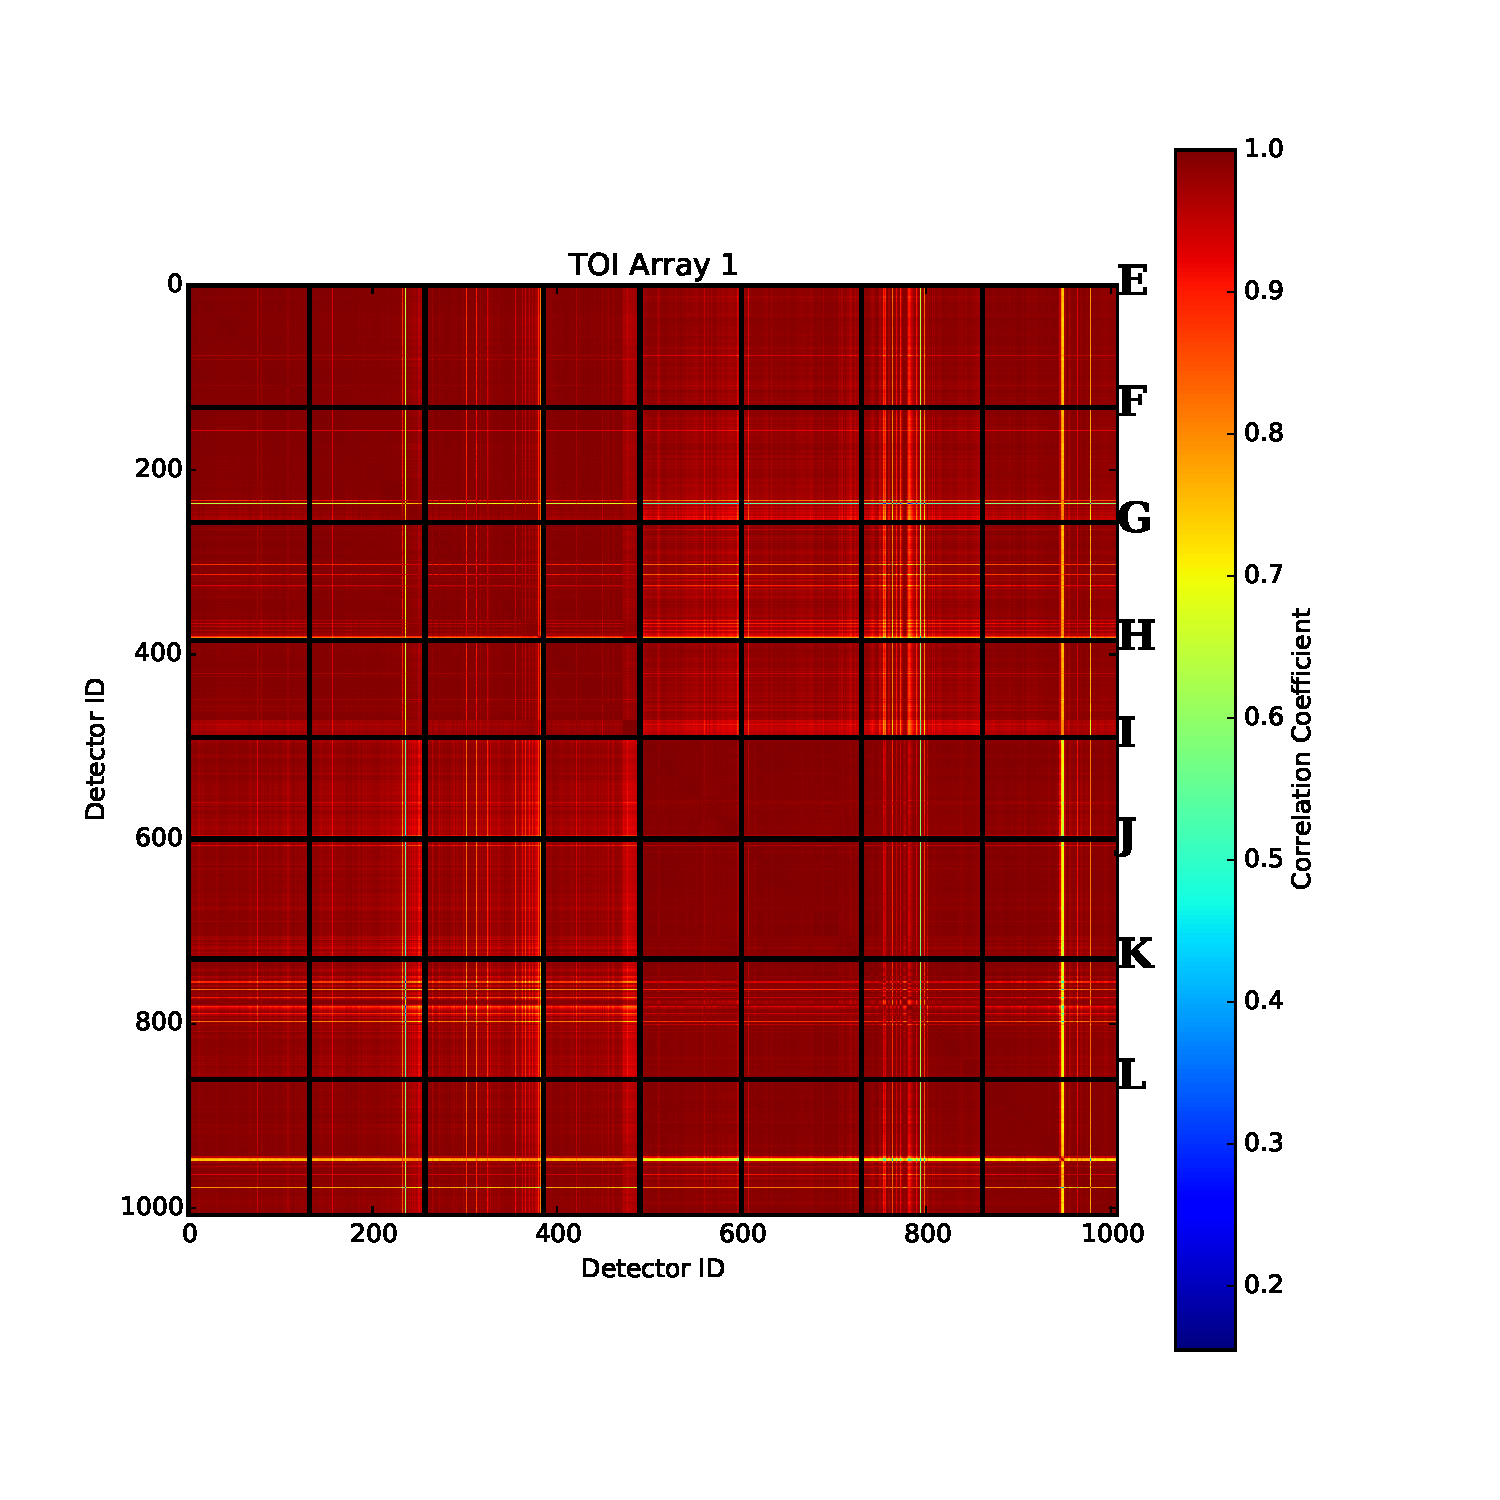
\includegraphics[width=0.3\textwidth]{Figures/NoiseTests/corrmat_TOI_array_1_20170228s151.pdf}
%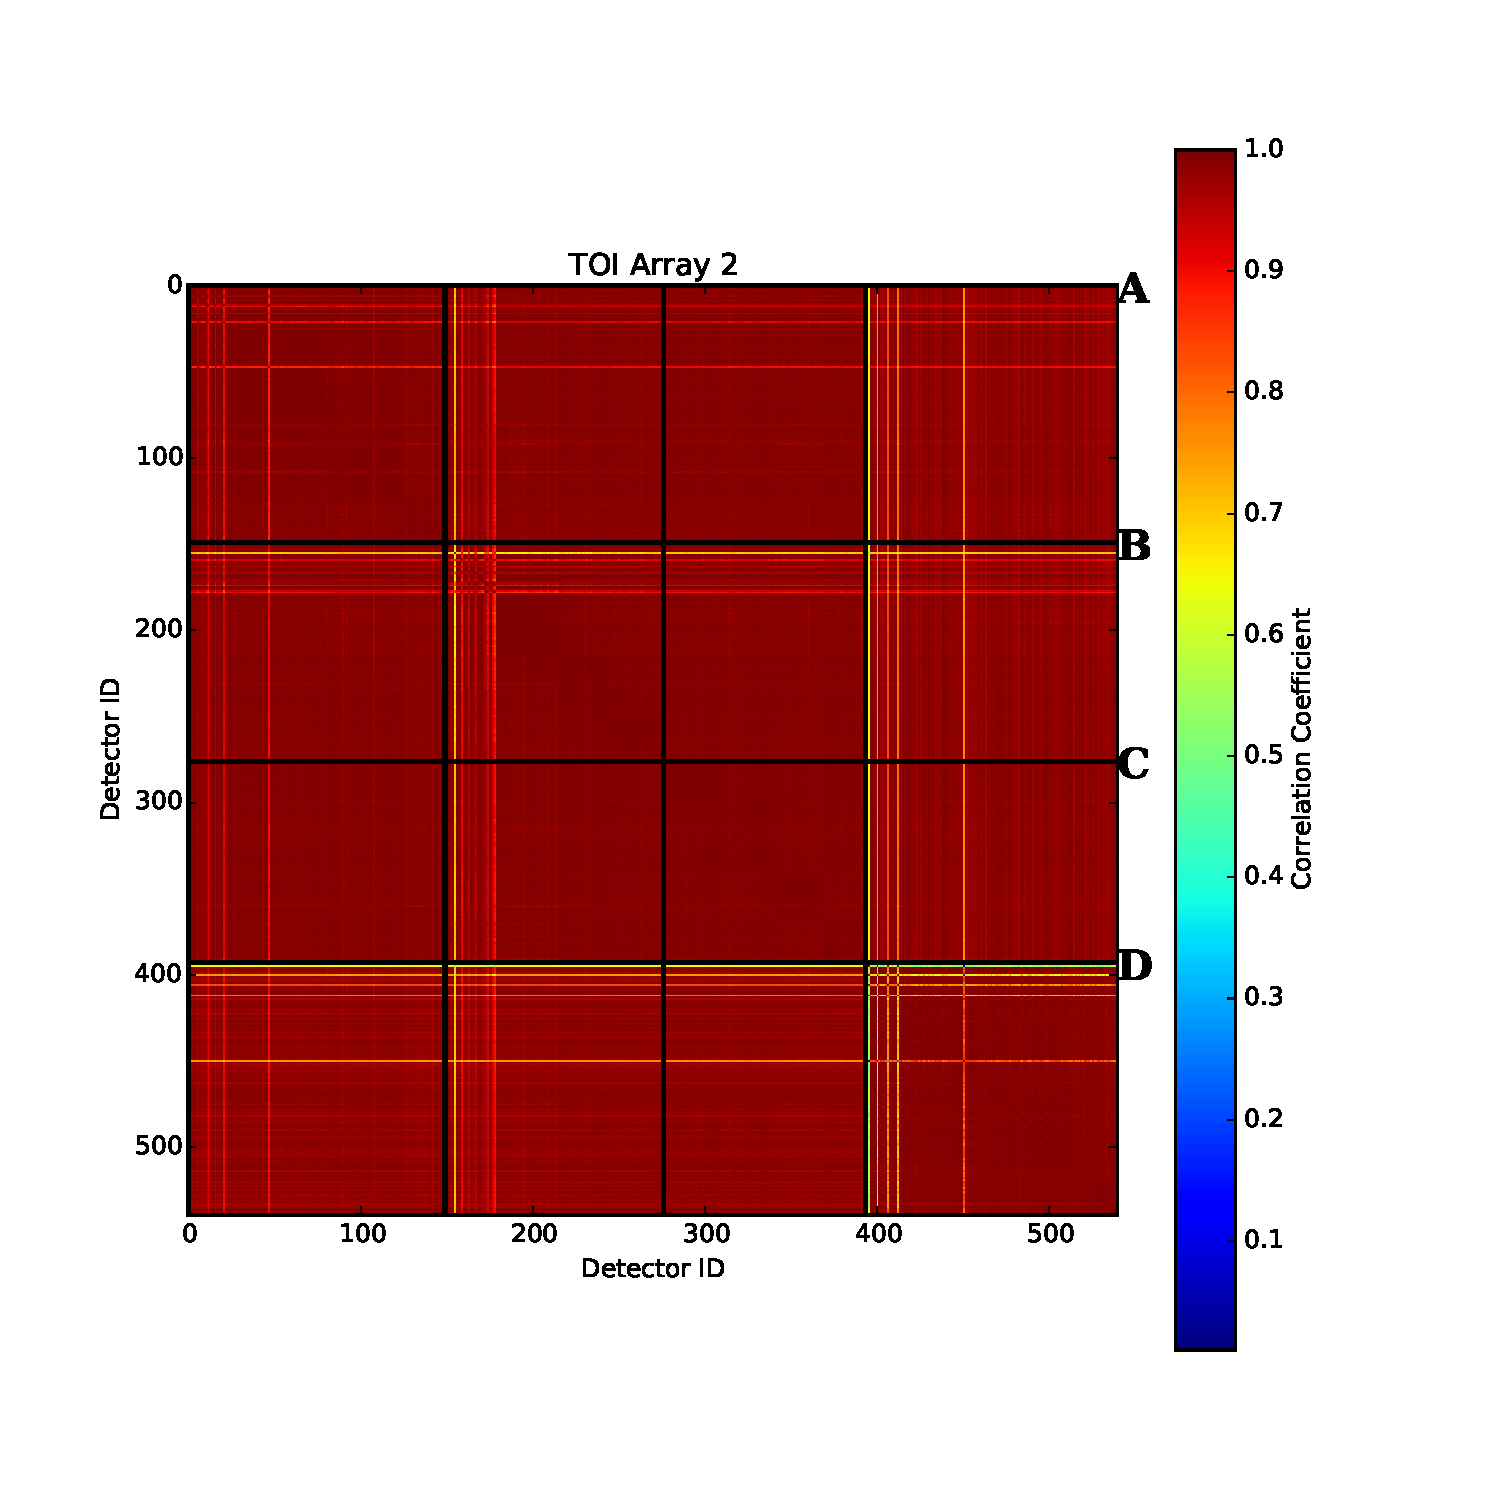
\includegraphics[width=0.3\textwidth]{Figures/NoiseTests/corrmat_TOI_array_2_20170228s151.pdf}
%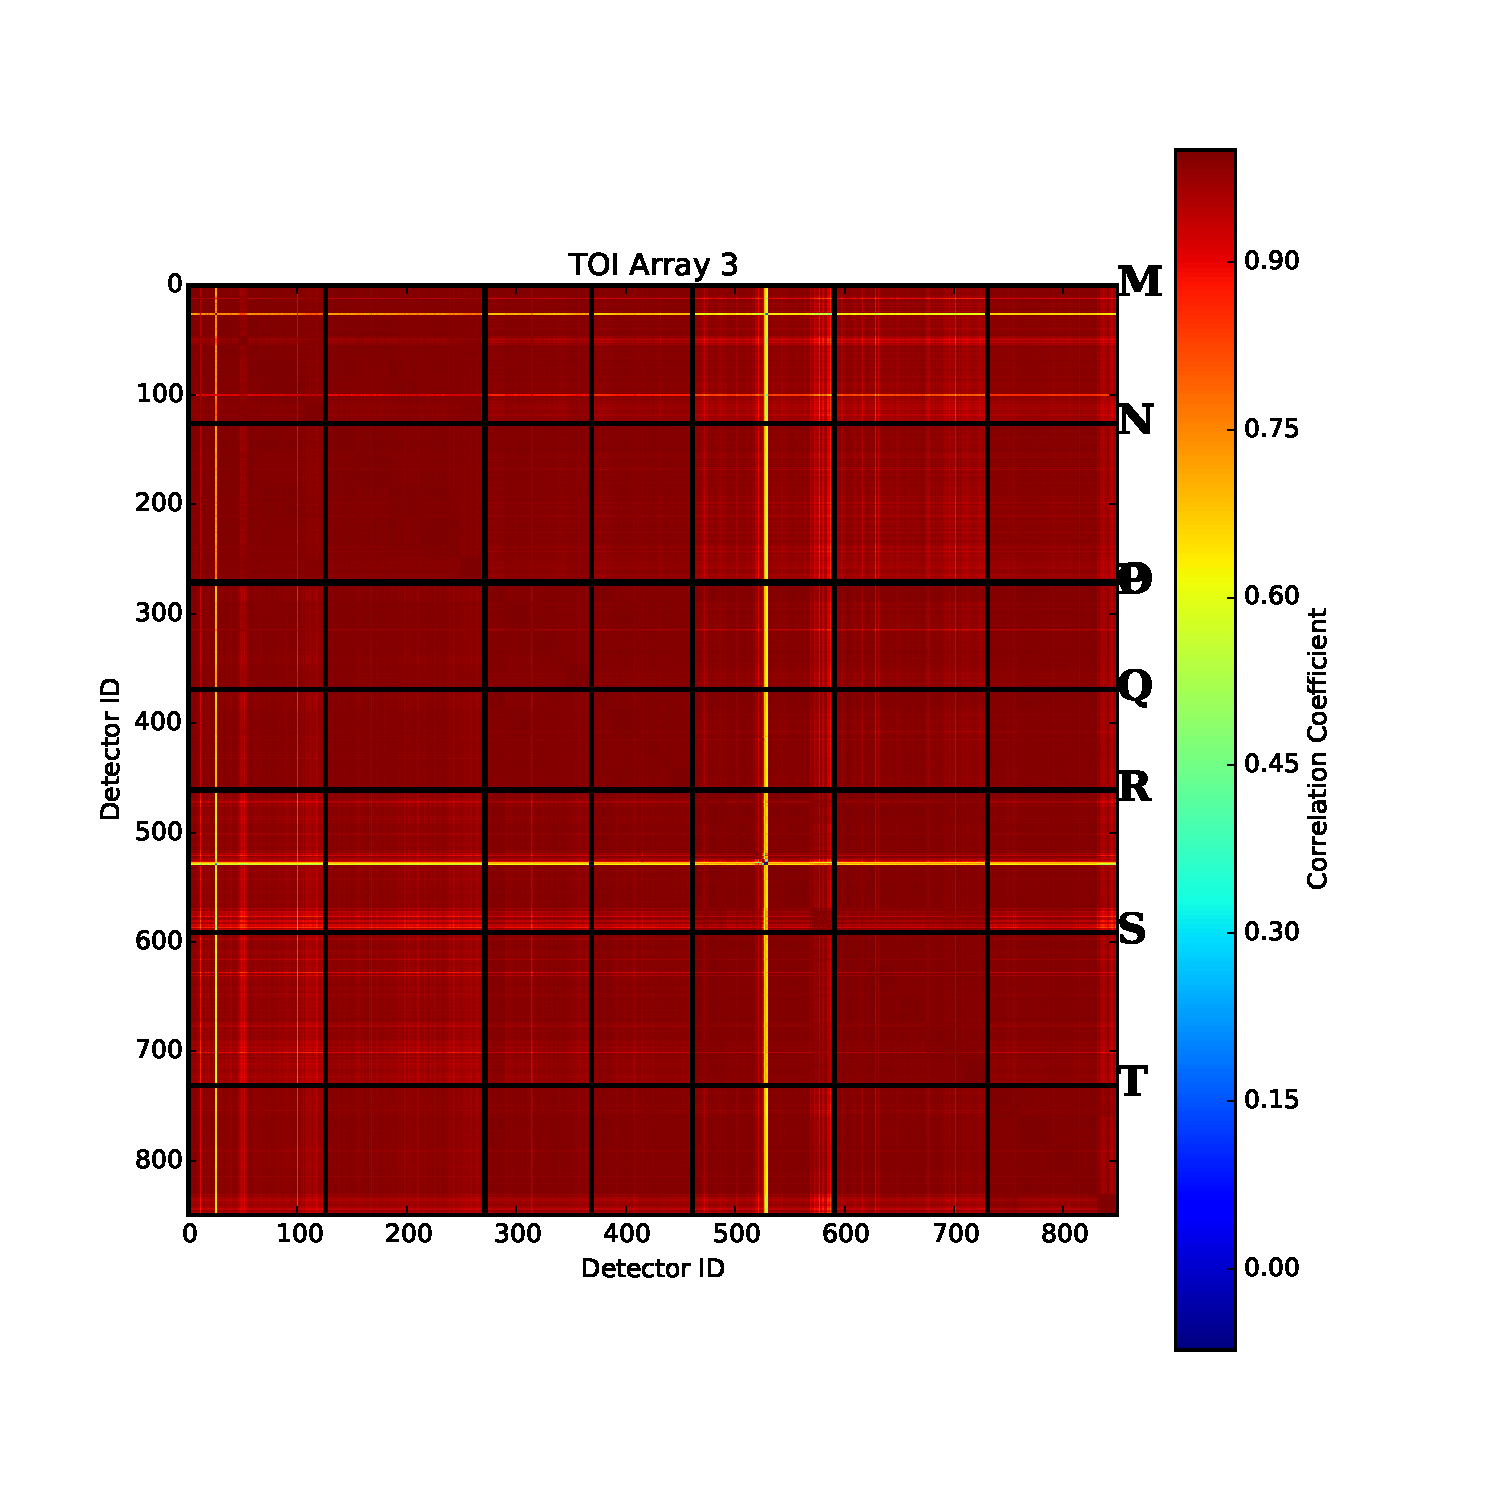
\includegraphics[width=0.3\textwidth]{Figures/NoiseTests/corrmat_TOI_array_3_20170228s151.pdf}
%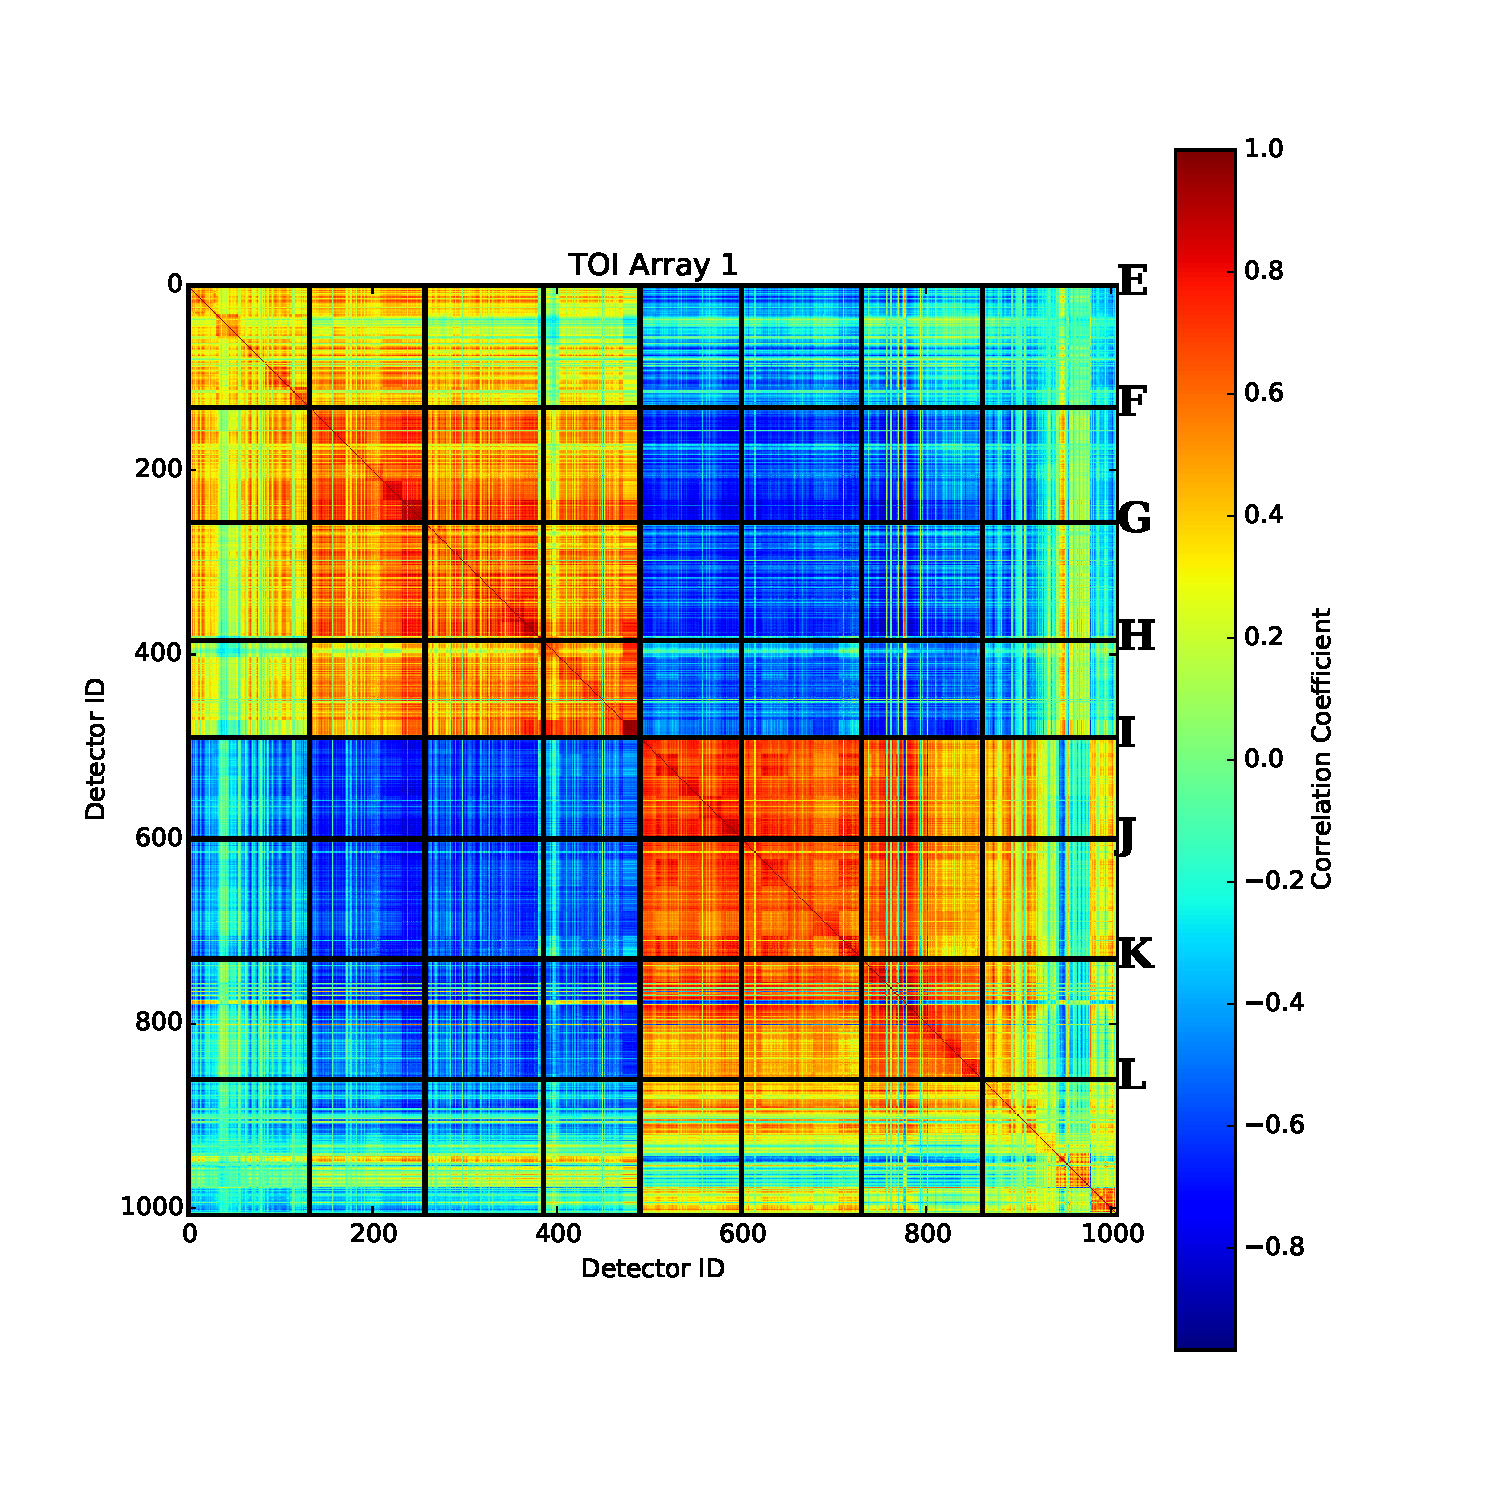
\includegraphics[width=0.3\textwidth]{Figures/NoiseTests/corrmat_TOI_CM_array_1_20170228s151.pdf}
%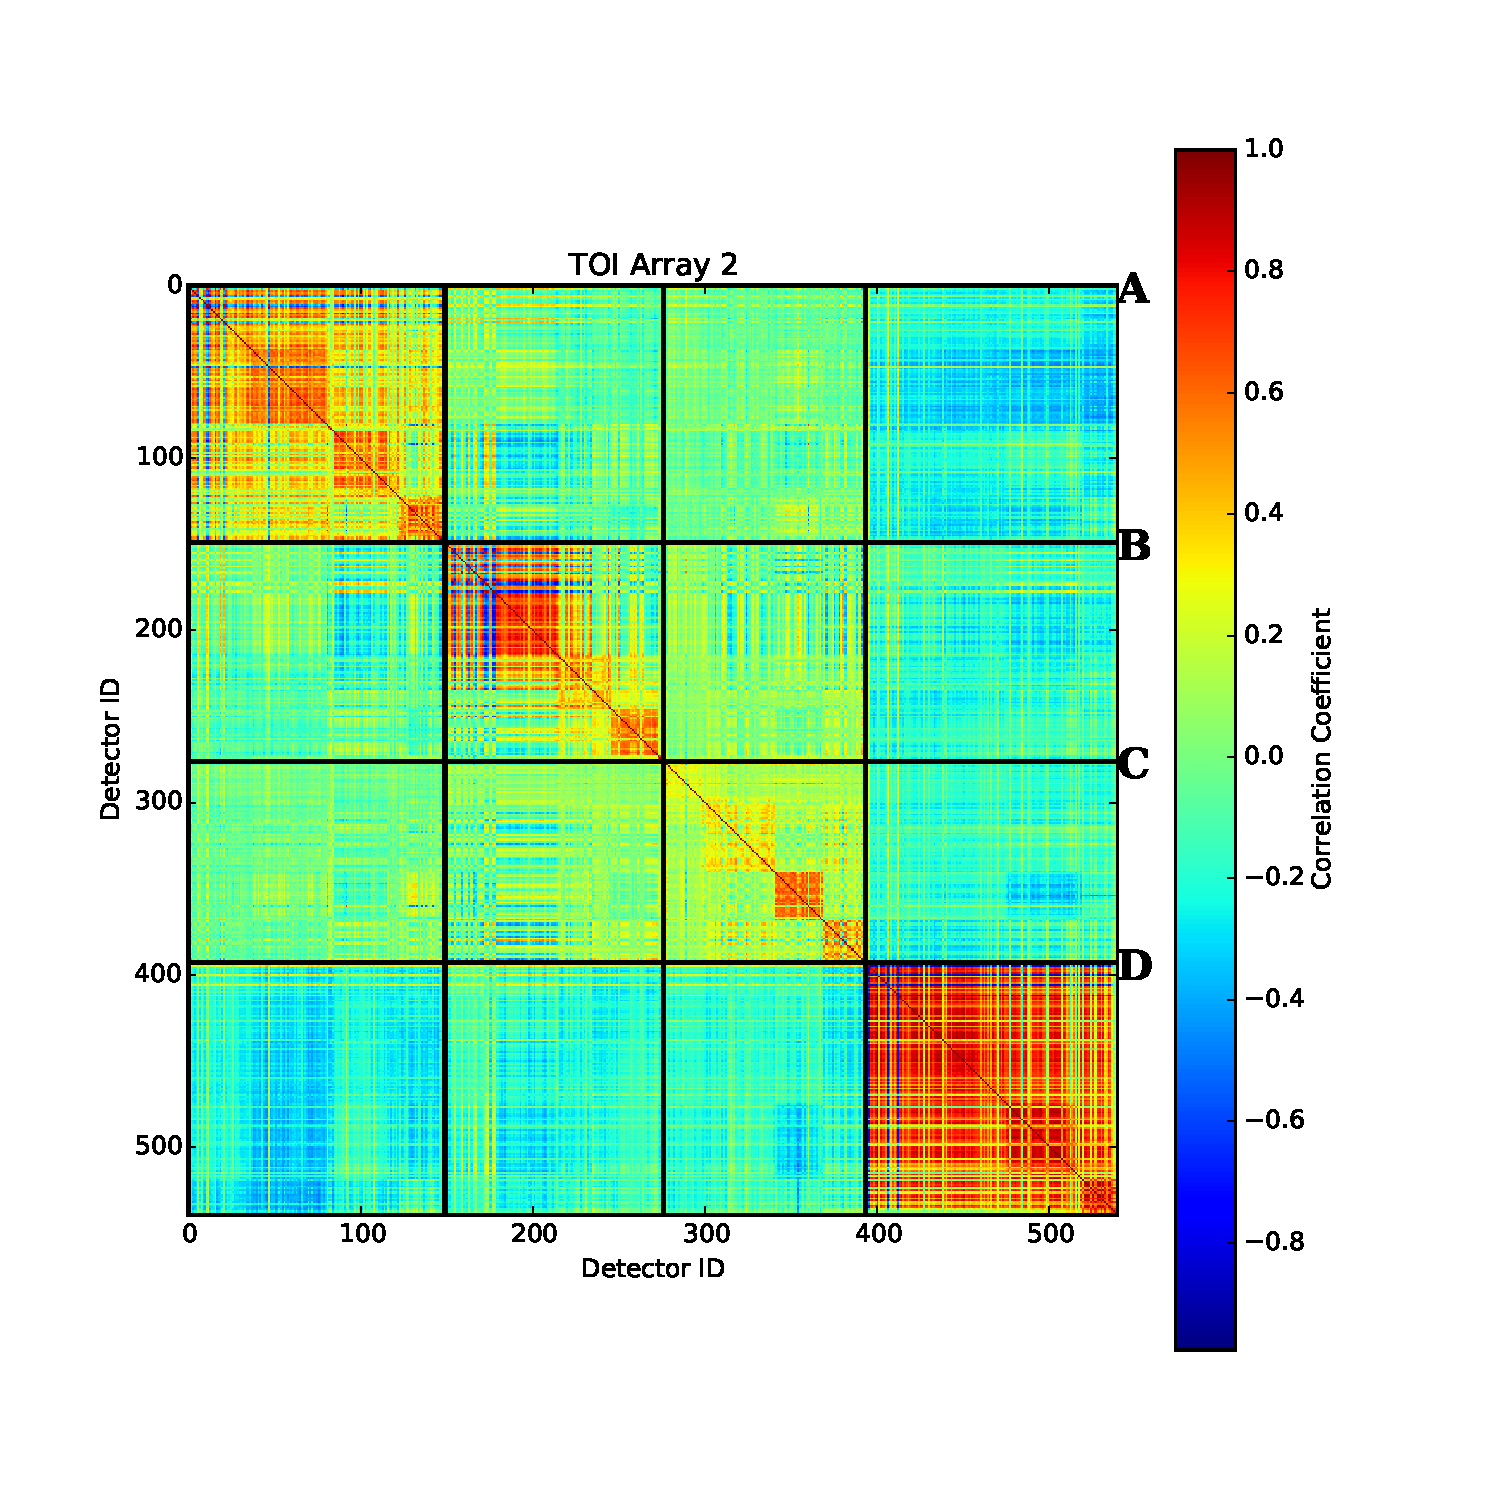
\includegraphics[width=0.3\textwidth]{Figures/NoiseTests/corrmat_TOI_CM_array_2_20170228s151.pdf}
%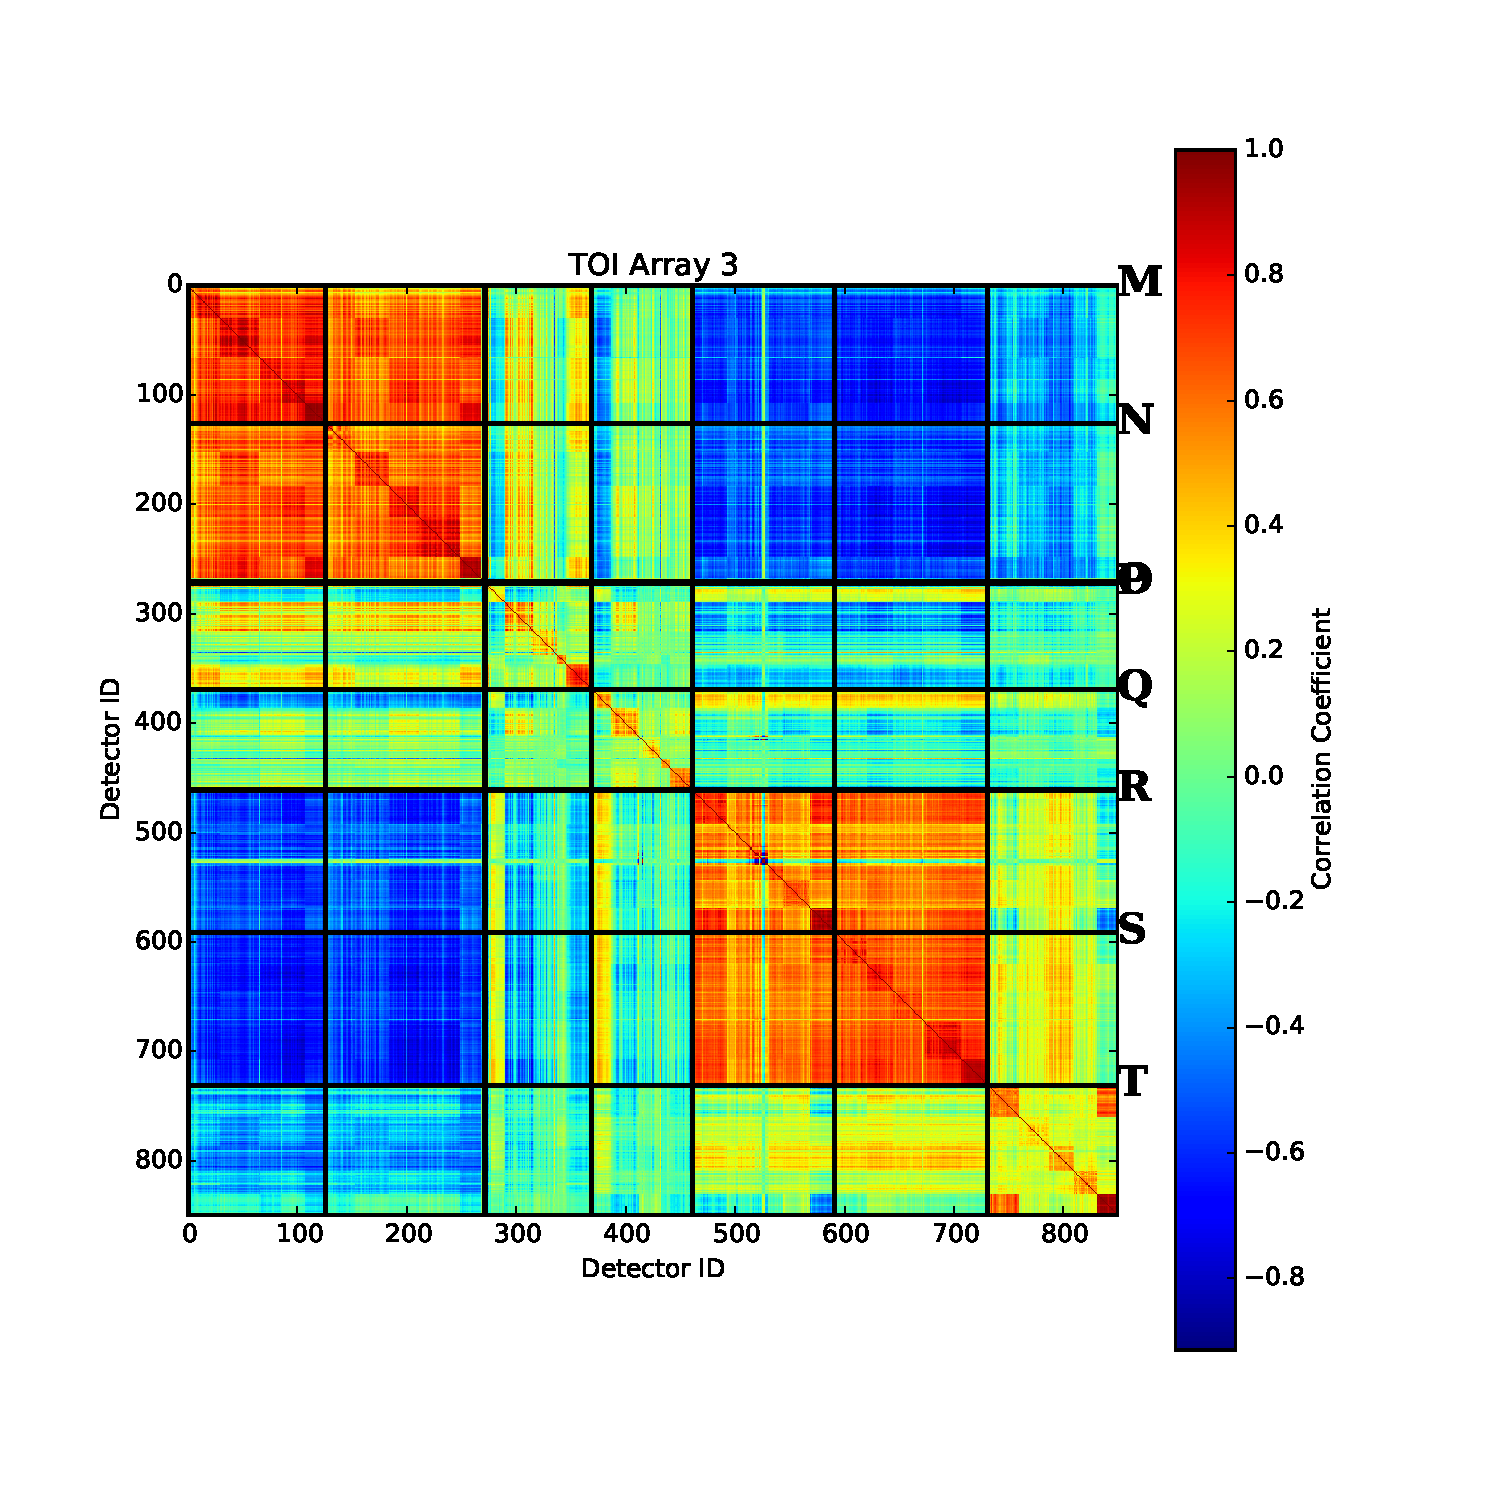
\includegraphics[width=0.3\textwidth]{Figures/NoiseTests/corrmat_TOI_CM_array_3_20170228s151.pdf}
%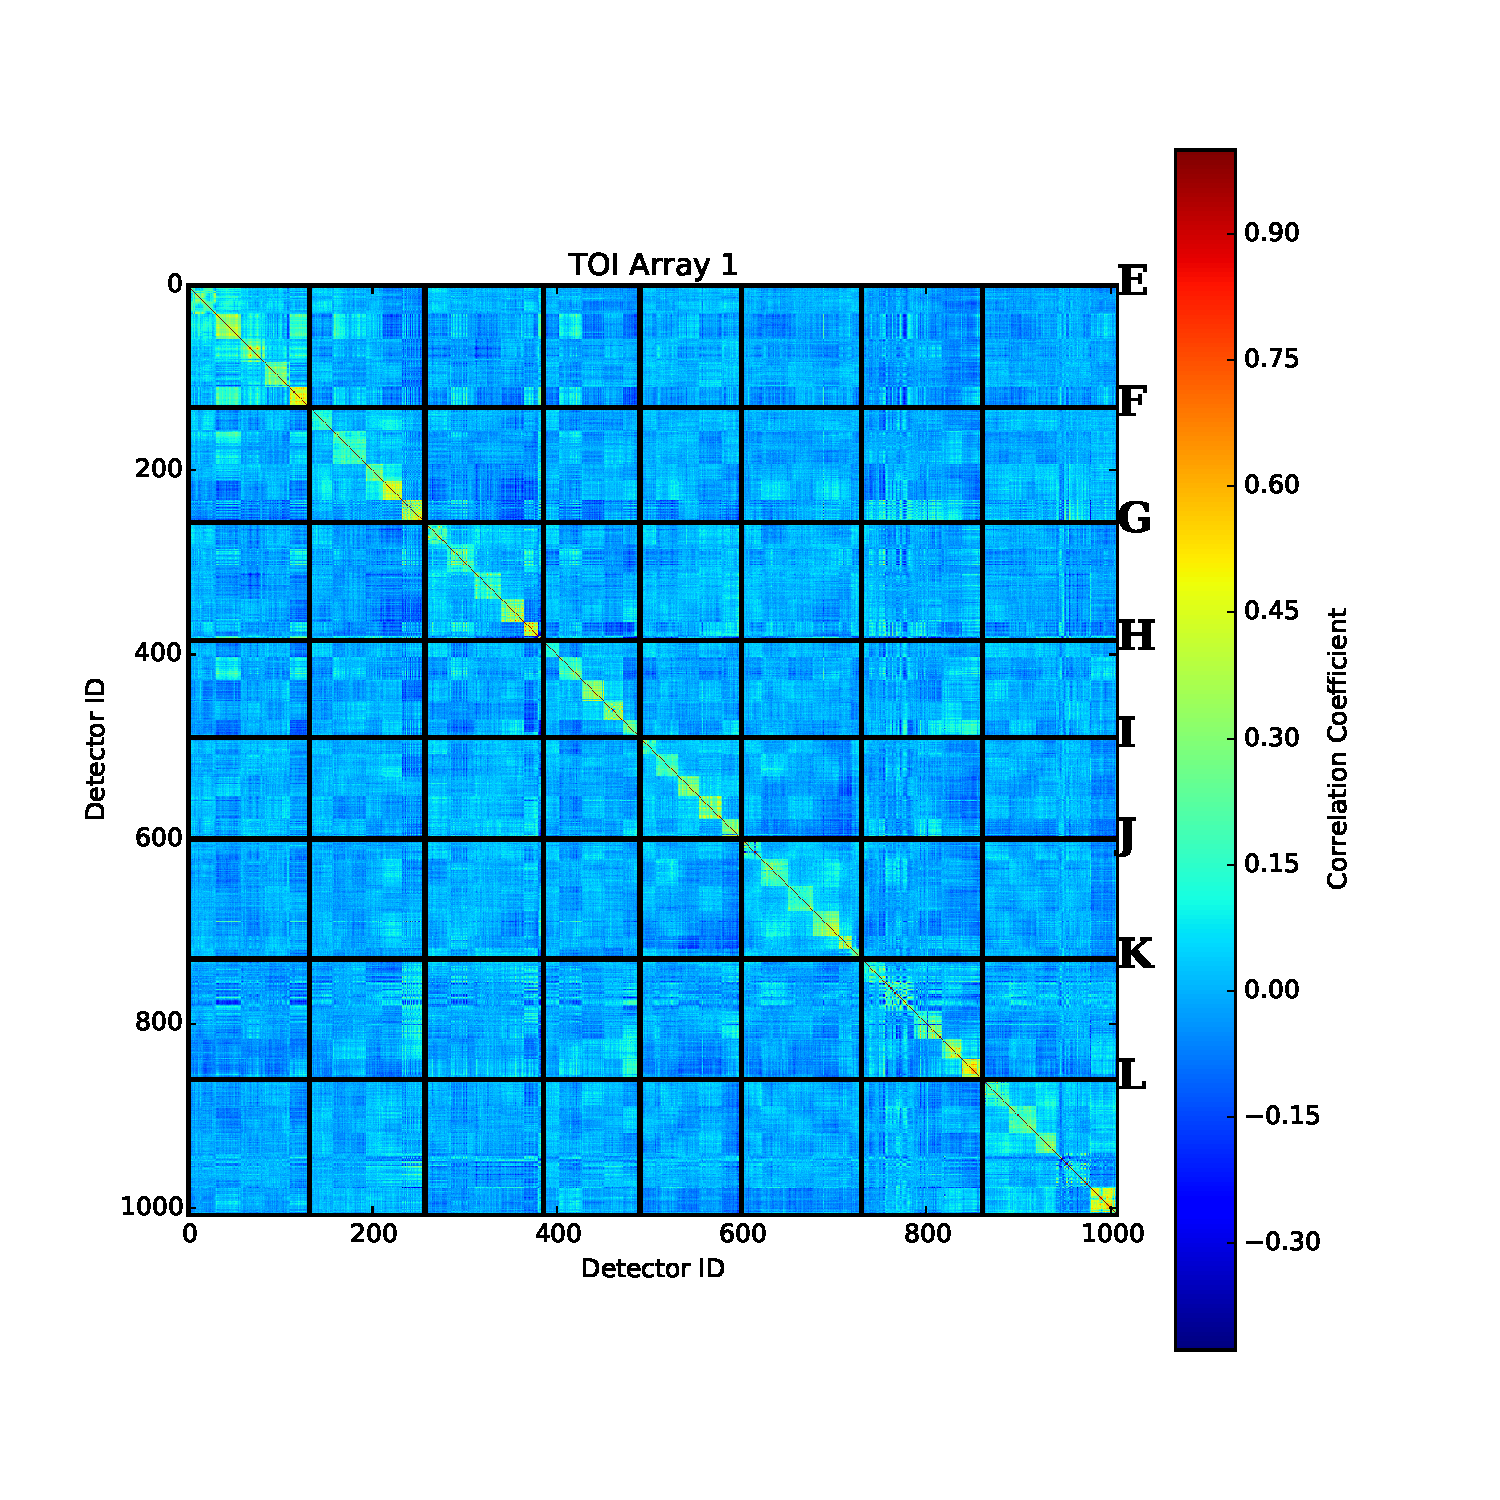
\includegraphics[width=0.3\textwidth]{Figures/NoiseTests/corrmat_TOI_PCA_array_1_20170228s151.pdf}
%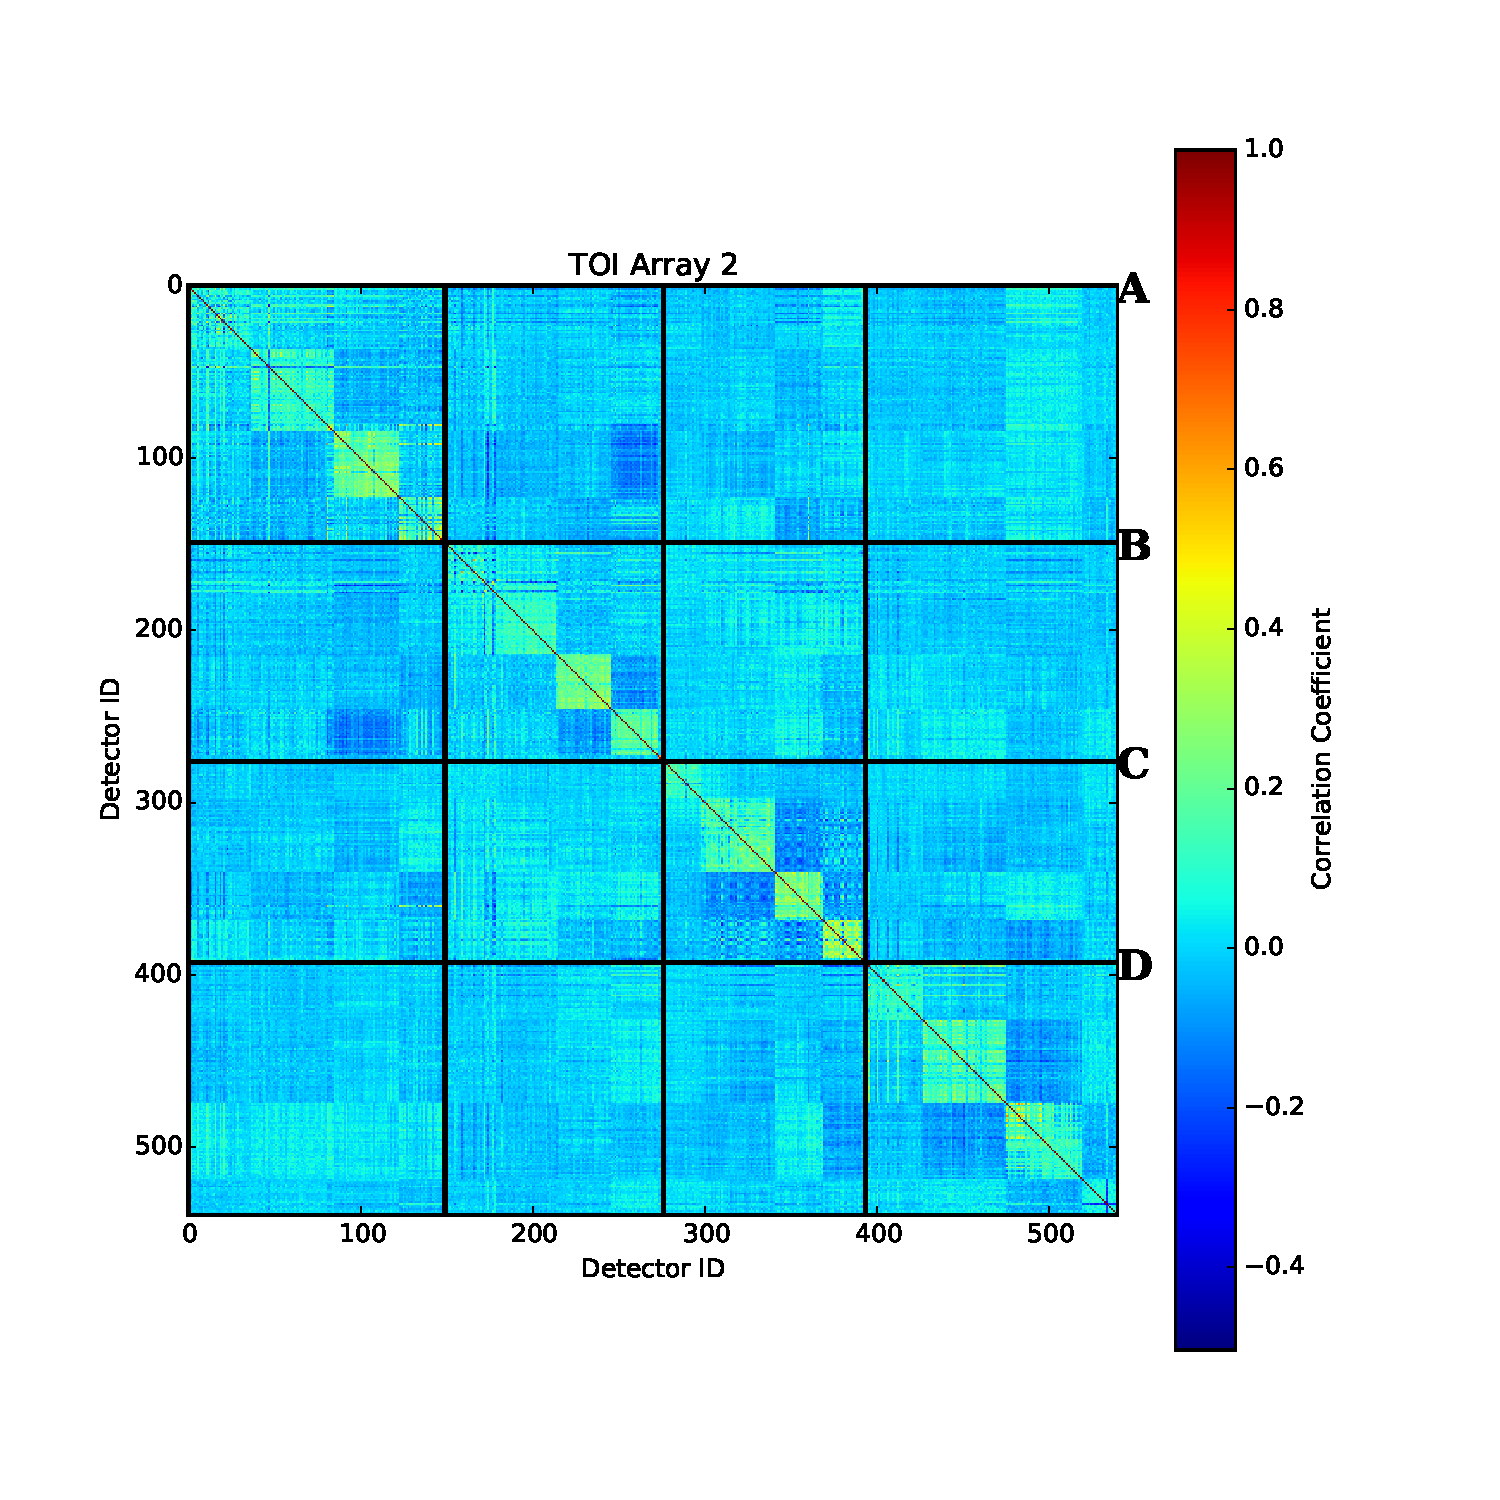
\includegraphics[width=0.3\textwidth]{Figures/NoiseTests/corrmat_TOI_PCA_array_2_20170228s151.pdf}
%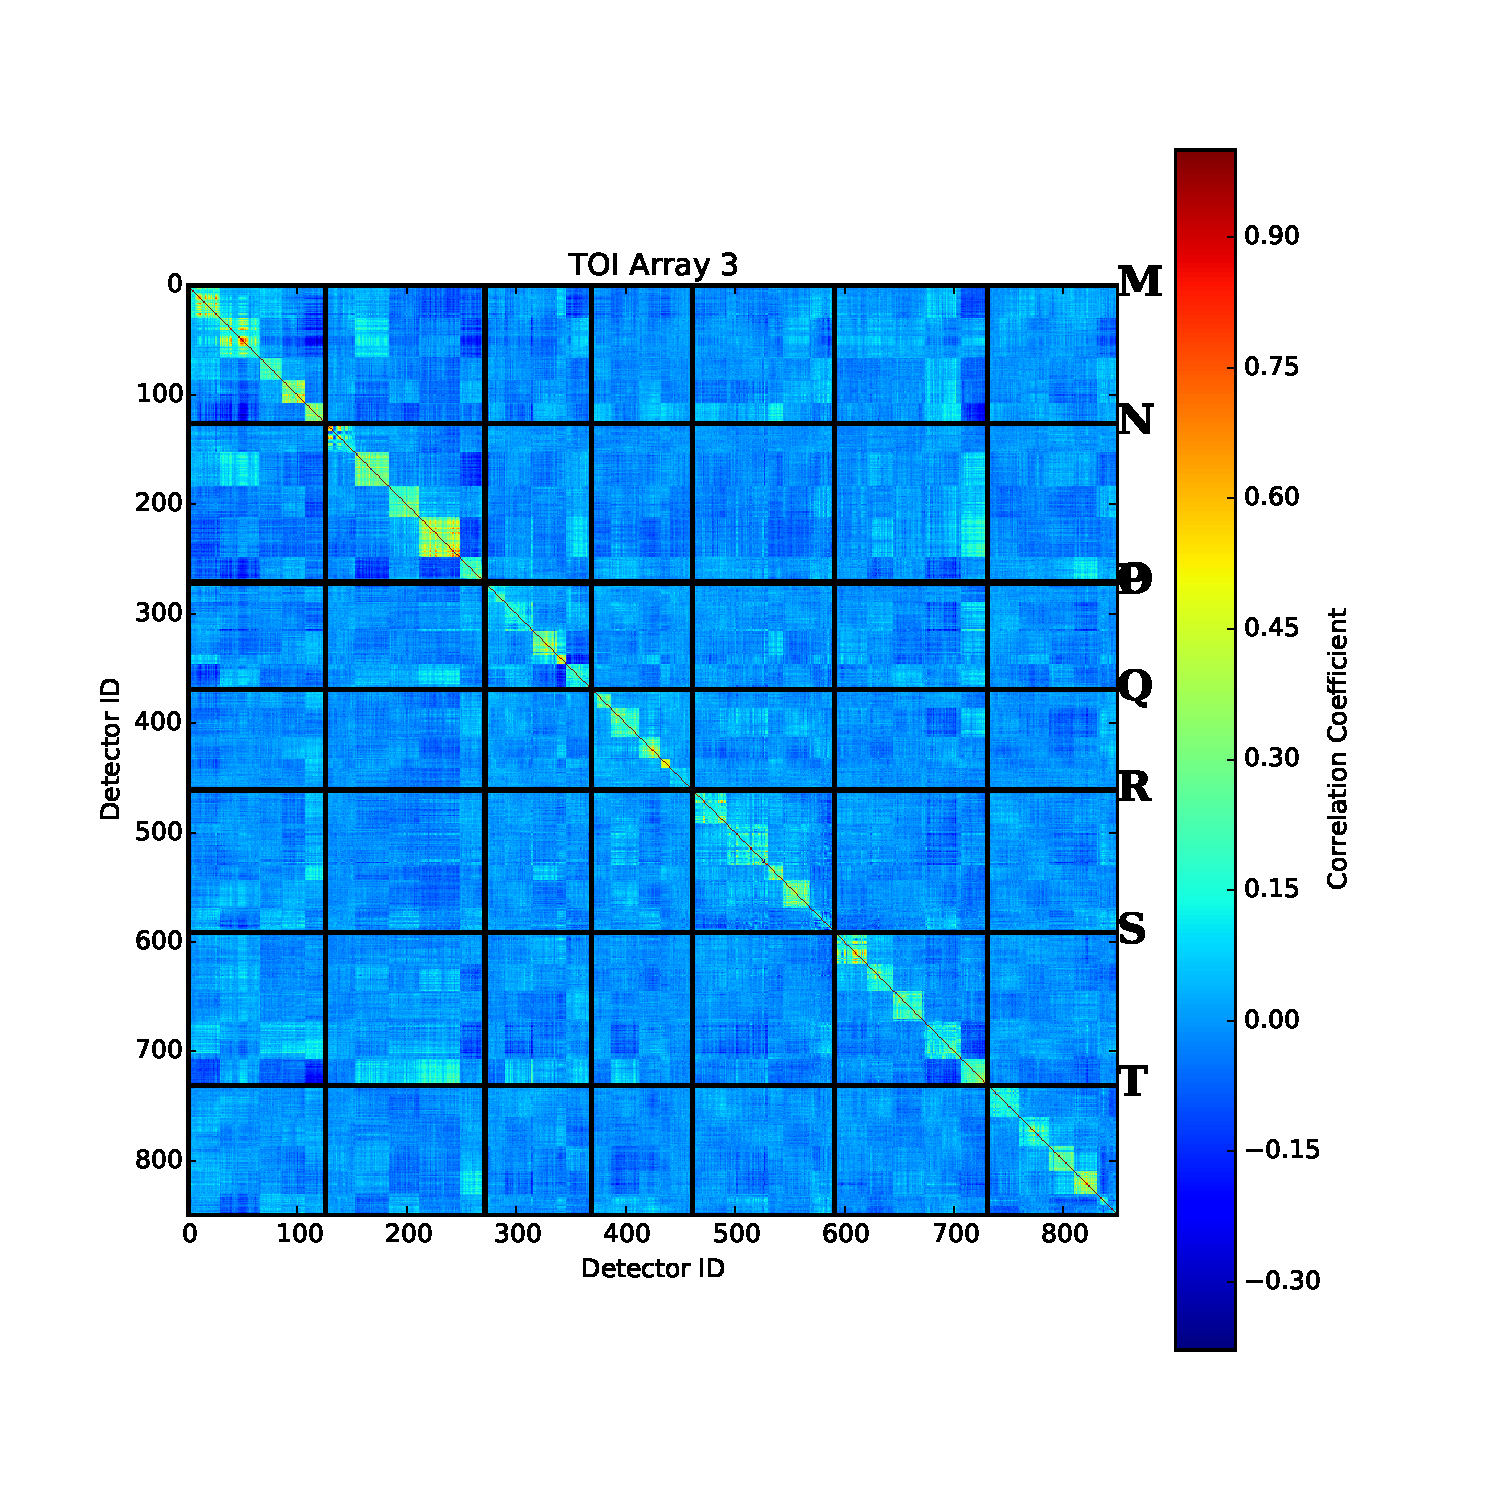
\includegraphics[width=0.3\textwidth]{Figures/NoiseTests/corrmat_TOI_PCA_array_3_20170228s151.pdf}
%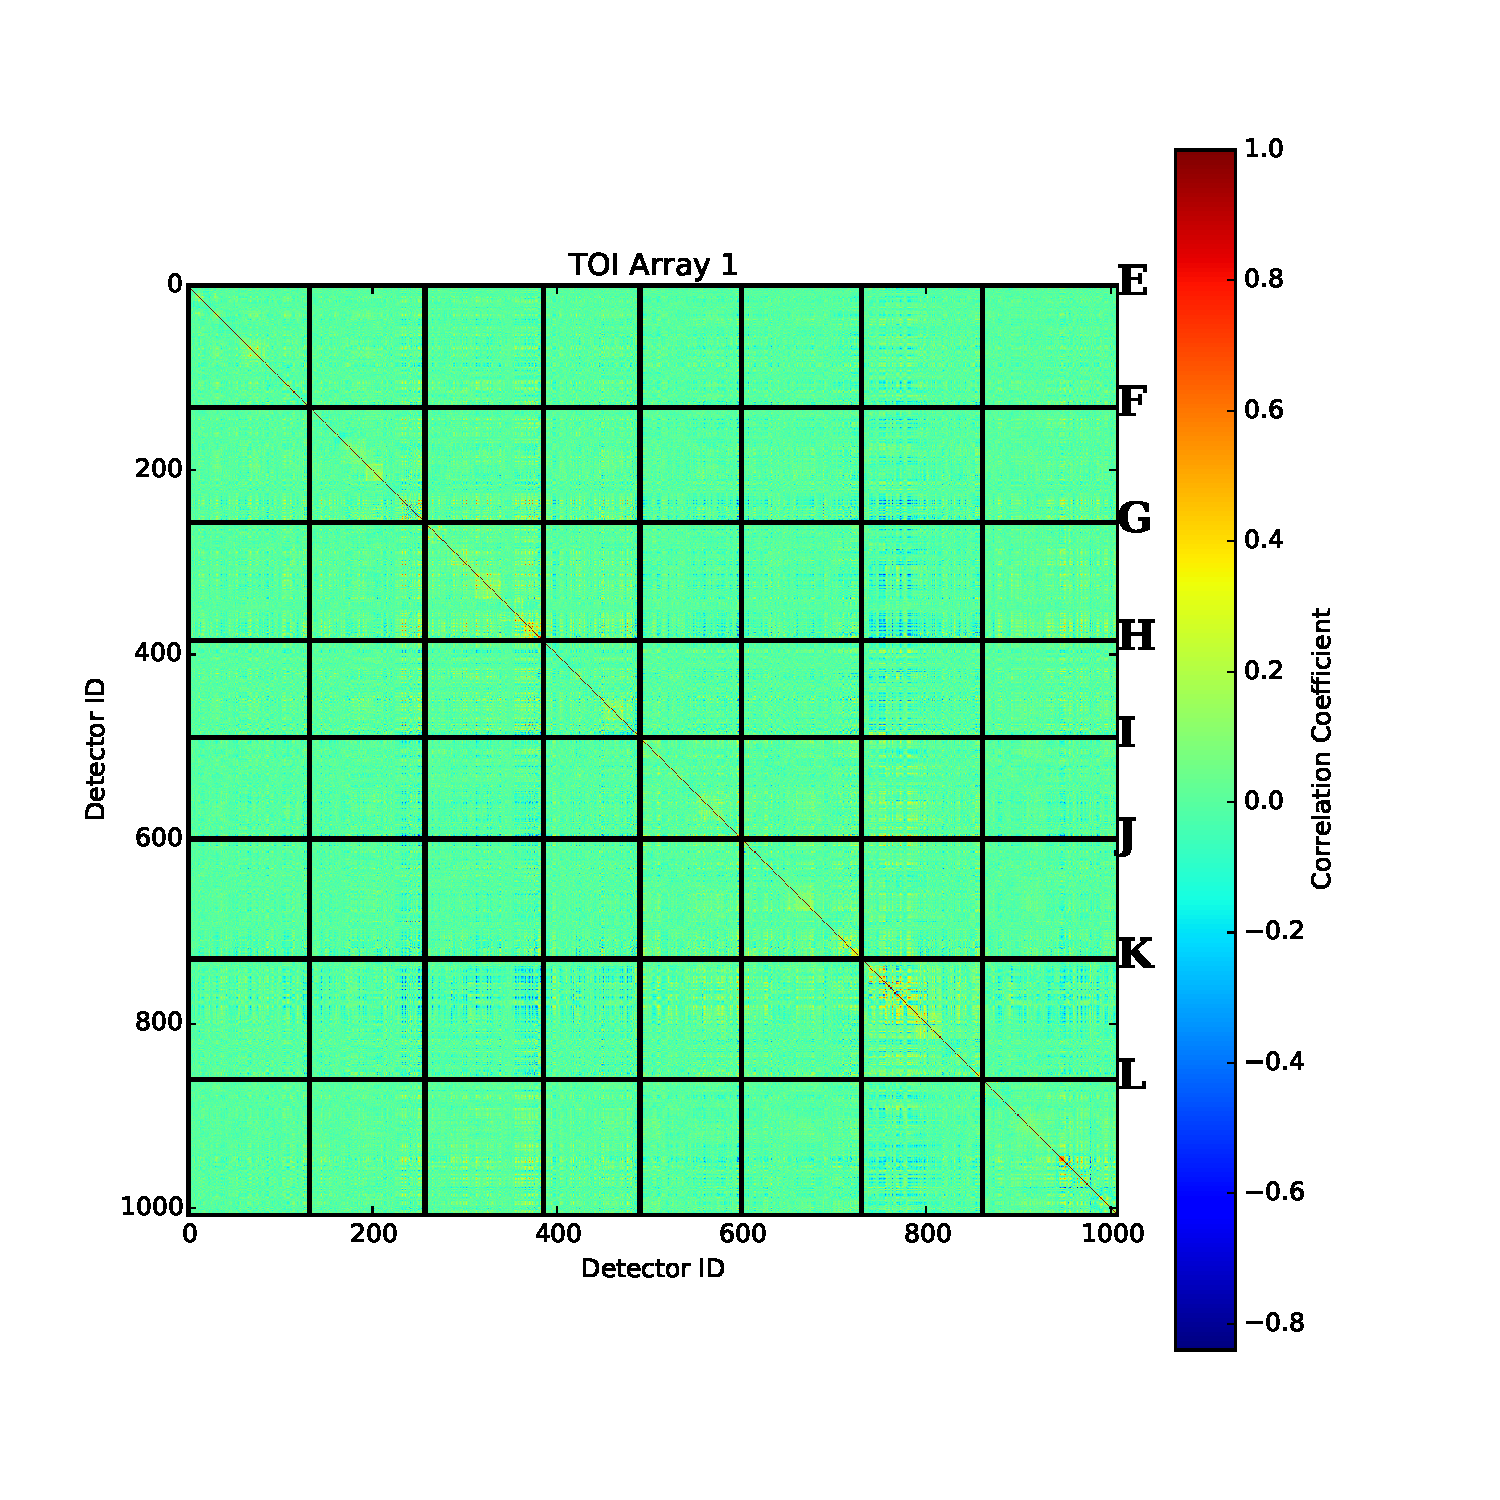
\includegraphics[width=0.3\textwidth]{Figures/NoiseTests/corrmat_TOI_BCP_array_1_20170228s151.pdf}
%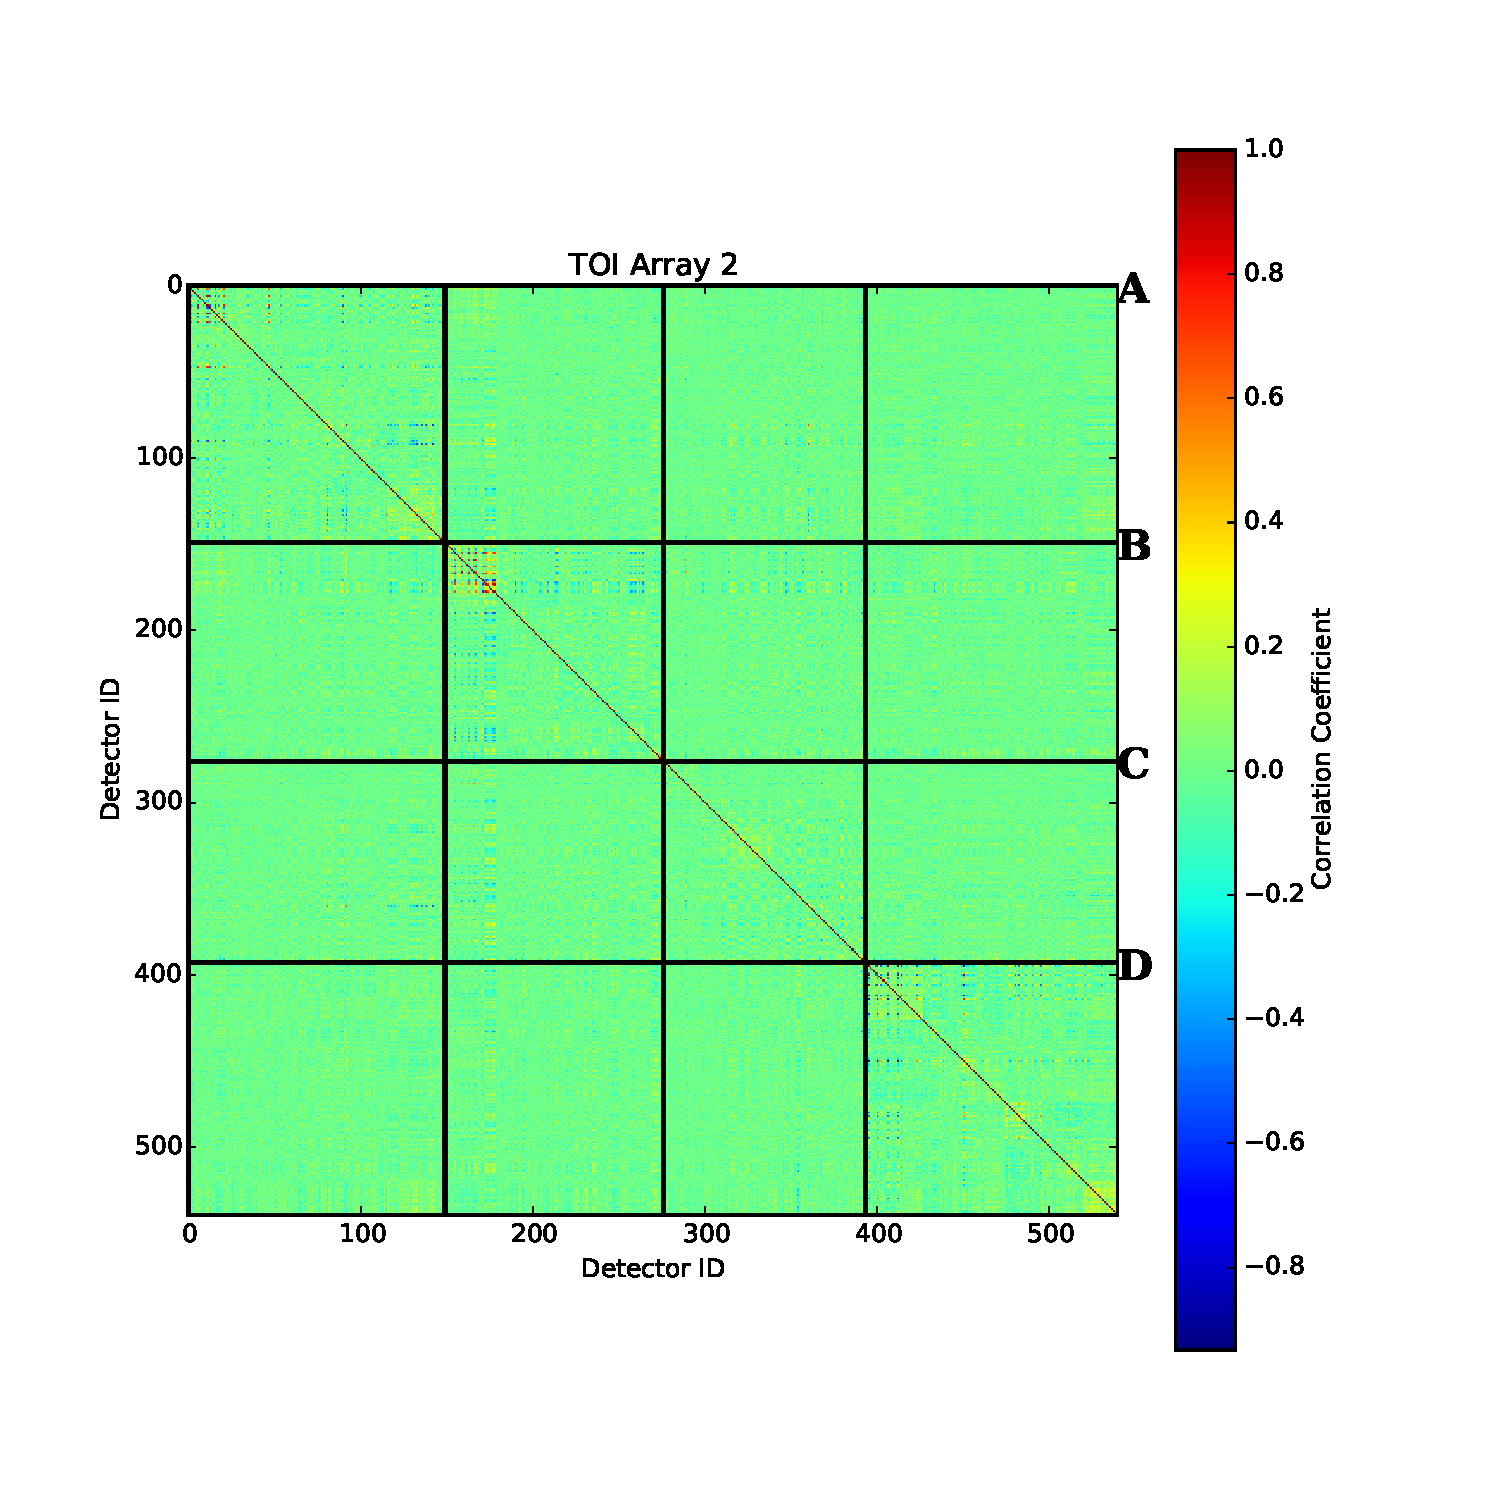
\includegraphics[width=0.3\textwidth]{Figures/NoiseTests/corrmat_TOI_BCP_array_2_20170228s151.pdf}
%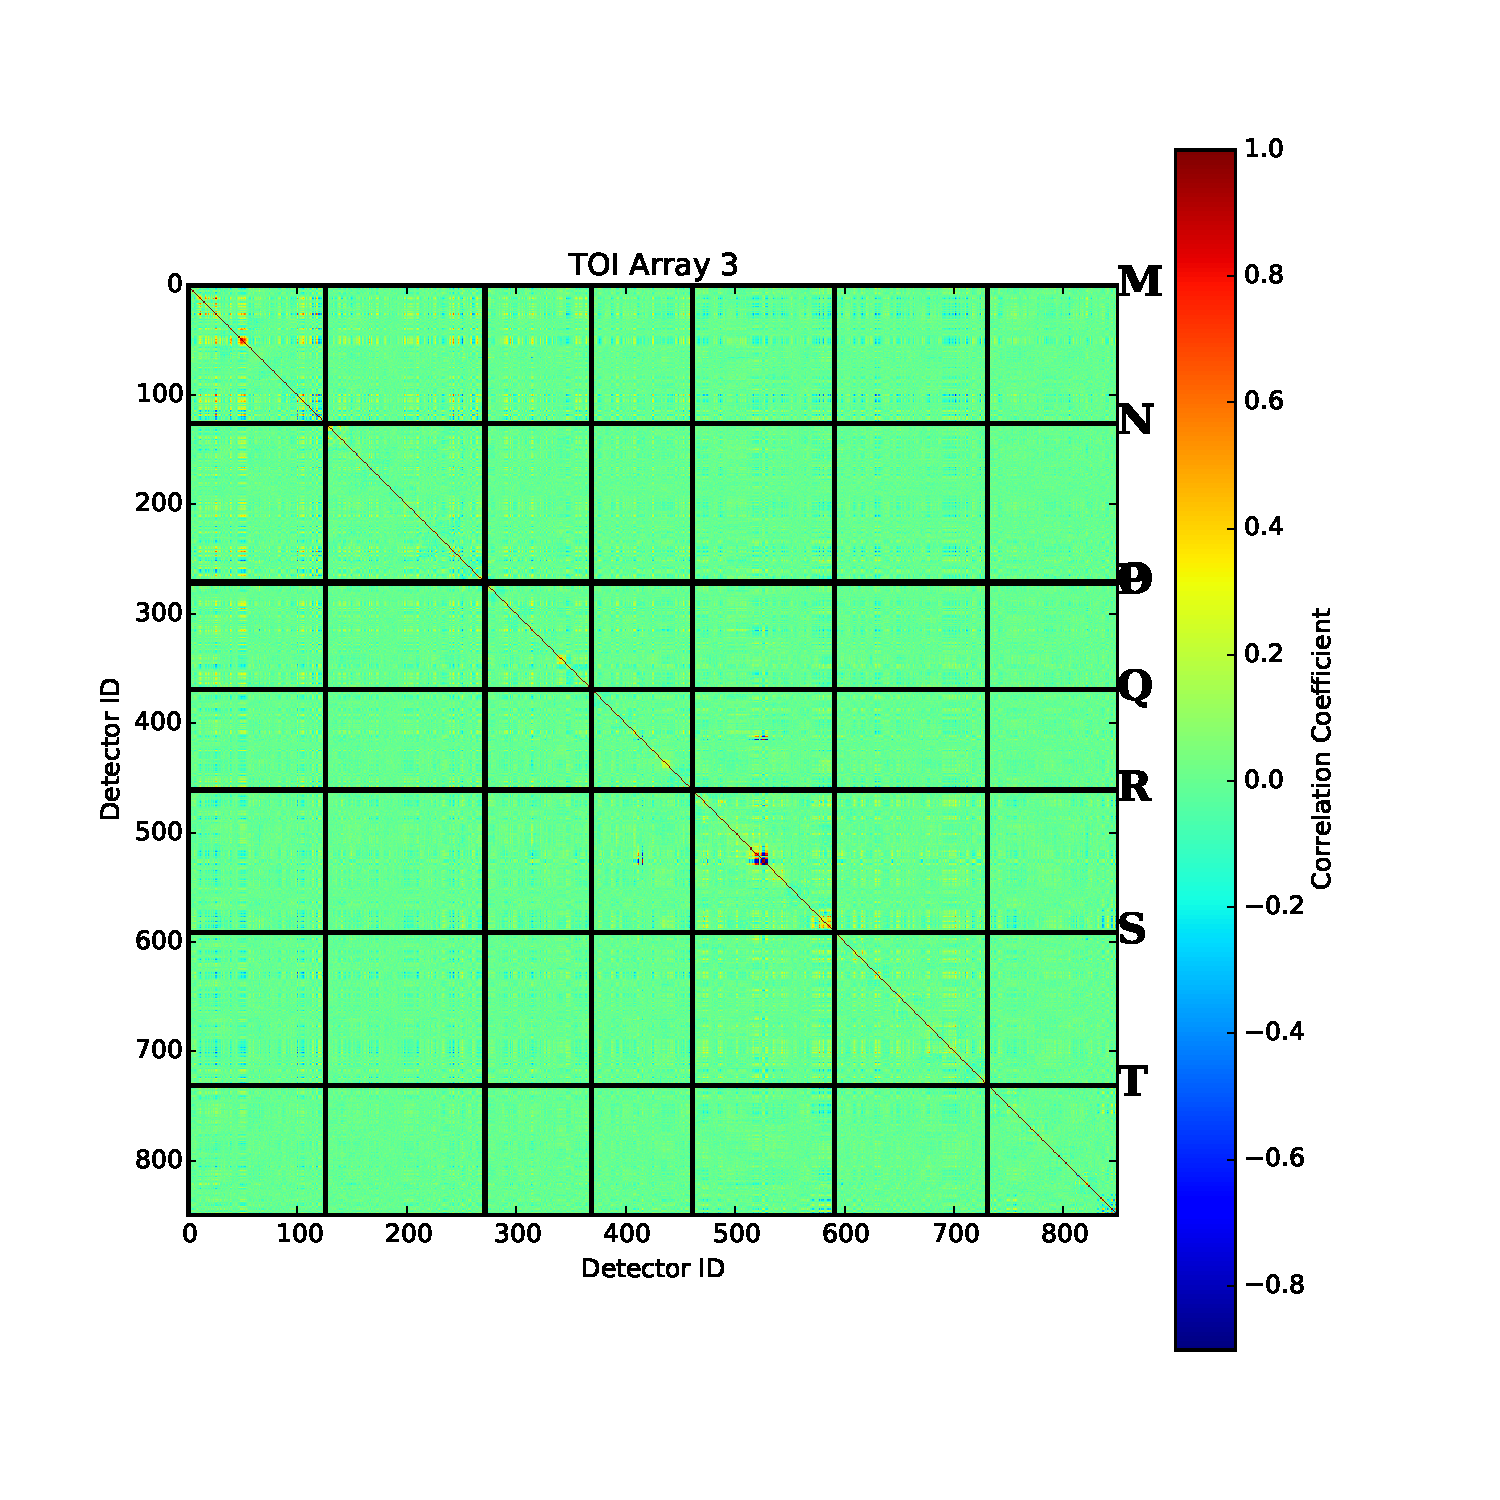
\includegraphics[width=0.3\textwidth]{Figures/NoiseTests/corrmat_TOI_BCP_array_3_20170228s151.pdf}
%\end{center}
%\caption[KID-to-KID correlation matrices]{\emph{From left to right:} TOI correlation
%  matrices for the three NIKA2 arrays (A1, A2, and A3) for scan
%  20170228s150. From top to bottom we present the correlation of the raw data,
%  after CM, PCA and MCP decorrelation methods. \label{corrmatrix}}
%\end{figure}
%
%As presented on Fig.~\ref{fig:nika_toi}, the atmosphere and the electronic noise
%combine into a large low frequency component that we want to eliminate as much
%as possible. Most of the atmospheric component is common to all KIDs, which is
%expected because the telescope is a $30\,\rm{m}$ dish and therefore
%has a near field limit at 900\,km.

As illustrated on the upper panel of Fig.~\ref{fig:nika_toi}, the
low-frequency noise component is seen by all KIDs at the same time,
while the astrophysical signal {\lp (Uranus in this case)} is shifted
from one KID to another.
{\lp In this figure the KID TOIs have been rescaled to be null
at $t=0$.} 
A simple average of the KID TOIs provides an
estimate of the low-frequency noise component, that we referred to as
a \emph{common mode}, while the signal is averaged out. The common
mode shown as a red line on the lower panel of
Fig.~\ref{fig:nika_toi}, is then subtracted to each KID TOI.

%On Fig.~\ref{fig:nika_toi}, the planet Uranus is visible in the TOIs and serves as
%guide to both the noise relative amplitude and the discussion about TOI
%processing in the following.

%On Fig.~\ref{corrmatrix}, we take a scan on Pluto
%where the signal is negligible compared to noise on the timescale of a scan to
%focus on the noise properties. We present the KID to KID timeline correlation
%matrices for the three arrays,

%In Fig.~\ref{rmspws} we present the noise power spectra of
%a typical datastream, 
%either before any data reduction or with
%different estimates of the low frequency component:

%\begin{itemize}
%\item {\bf Common Mode decorrelation (CM)}. We use all detectors of the same
%  array to build an average low frequency component nicknamed \emph{common
%    mode}. This mode is then linearly regressed and subtracted from each KID
%  timeline. In this method, the \emph{common mode} at time $t$ is the median of
%  all KIDs at this time $t$.
%
%\item {\bf Principal Component Analysis (PCA)}. For each NIKA2 array
%  independently we decompose the covariance matrix in principal components. From
%  those we derive up to 10 independent templates corresponding to the largest
%  eigenvalues that we subtract from the TOIs.
%
%\item {\bf Most correlated pixels (\cmoneb)}. For each detector in a given array we
%  identify the detectors that are most correlated to it (a minimum of
%  15). Using those detectors we compute a common mode like in method CM but with
%  more refinements to be valid even on bright sources (see below).
%\end{itemize}

% We observe that after decorrelation we reduce significantly the rms of the
%noise. Equivalently, the $1/f$-like noise in the power spectra
%(principally due to atmospheric emission)
%is significantly reduced leading to nearly flat spectra down to 0.05 Hz, with
%larger $1/f$-like residual noise for the CM decorrelation method at lower
%frequencies. This is translated into a larger rms noise for this method with
%respect to the others. For the three arrays we find increasing noise with
%increasing resonant frequency within each electronic box. This is probably
%related to the difference of gains between subbands in the readout
%electronics. %We also find for the three arrays some noise bursts that are not
%fully consistent from one decorrelation method to another. 

%Studies of the KID to KID timeline correlation matrices
%As expected the raw data noise correlation is dominated by atmospheric
%noise and we observe full correlation between detectors but for badly
%behaving detectors which are removed from the analysis.
%Significant residual correlation and anti-correlation is
%observed after CM decorrelation. This is both due to spatial changes in the
%atmospheric emission (overall residuals) and to instrumental and electronic
%noise characteristics (correlation blocks that can be associated to electronic
%boxes).  The PCA decorrelation leads to approximately block-diagonal correlation
%matrices. These observed blocks in the correlation matrix can be associated to
%first order to the different sub-bands in each of the electronic boxes. In the
%case of the MCP decorrelation, for which only those pixels highly correlated to
%the pixel of interest are used, we observe that the correlation matrix is more
%diagonal than in the two other derivations of the common mode.

\begin{figure}[ht!] % Inline image example
  \begin{center}
    % A1
%    \begin{overpic}[clip=true, trim={0.5cm, 0, 0, 0.6cm},width=0.59\textwidth]{Figures/NoiseTests/rms_TOI_array_1_20170228s151_mod.pdf}
%      \put(3,5){\rotatebox{90}{\scriptsize Noise RMS [arbitrary units]}}
%  \end{overpic}
    \begin{overpic}[clip=true, trim={0.5cm, 0, 0, 0.5cm},width=0.40\textwidth]{Figures/pws_TOI_array_1_20170228s151_mod.pdf}
      \put(2,15){\rotatebox{90}{\scriptsize P$_{\nu}$ [arbitrary units]}}
  \end{overpic}
% A3
%    \begin{overpic}[clip=true, trim={0.5cm, 0, 0, 0.5cm},width=0.59\textwidth]{Figures/NoiseTests/rms_TOI_array_3_20170228s151_mod.pdf}
%      \put(3,5){\rotatebox{90}{\scriptsize Noise RMS [arbitrary units]}}
%    \end{overpic}
    \begin{overpic}[clip=true, trim={0.5cm, 0, 0, 0.5cm},width=0.40\textwidth]{Figures/pws_TOI_array_3_20170228s151_mod.pdf}
      \put(2,15){\rotatebox{90}{\scriptsize P$_{\nu}$ [arbitrary units]}}
    \end{overpic}
    % A2
%    \begin{overpic}[clip=true, trim={0.5cm, 0, 0, 0.6cm},width=0.59\textwidth]{Figures/NoiseTests/rms_TOI_array_2_20170228s151_mod.pdf}
%      \put(3,5){\rotatebox{90}{\scriptsize Noise RMS [arbitrary units]}}
%    \end{overpic}
    \begin{overpic}[clip=true, trim={0.5cm, 0, 0, 0.5cm},width=0.40\textwidth]{Figures/pws_TOI_array_2_20170228s151_mod.pdf}
      \put(2,15){\rotatebox{90}{\scriptsize P$_{\nu}$ [arbitrary units]}}
    \end{overpic}
  \end{center}
\caption[Noise power spectra]{
  The data noise power spectra are shown for the three NIKA2 arrays (A1, A3, and
  A2 from top to bottom). % for scan 20170228s151.
  The power spectra are given for the raw
  data (blue), and for noise decorrelated data using the common mode
  (labeled CM, green), the PCA (red) and the \cmoneb\ (labeled MCP,
  cyan) methods.
  \label{rmspws}}
\end{figure}

{\lp For the calibration and performance assessment, we use an
atmospheric and electronic noise
decorrelation method named \cmoneb\, which comprises two
additional technicalities with respect to the common mode
method.} First, the signal contamination of the common mode estimate
is mitigated by discarding on-source KID data samples before averaging
the rescaled TOI. Second, instead of a single common mode subtraction to
all KIDs, we estimate an accurate common mode for each
KID. Calculating the KID-to-KID cross-correlation matrix, we
identify the most correlated KIDs. Then, we build an
inverse noise weighted co-addition of the timelines of the %off-source
KIDs that are the most correlated with the KID under
concern. Furthermore, we have tested on simulations that this method
does preserves the flux of {\lp point-like or moderately extended sources.}
% Regarding very extended sources (over more
%than a few arcminutes), the noise decorrelation requires iterative or
%more evolved methods, as will be discussed in \citet{Ponthieu2019}.}

In Fig.~\ref{rmspws} we present the noise power spectra of
a typical KID TOI both before any data reduction and using three noise
decorrelation methods, which are the simple common mode (CM) method
used in Fig.~\ref{fig:nika_toi}, a method based on a principal component
analysis (PCA) and the \cmoneb\ method (MCP). We observe that after decorrelation the
$1/f$-like noise in the power spectra (principally due to atmospheric
emission drifts)
is significantly reduced leading to nearly flat spectra down to {\lp 0.5~Hz}, with
lower $1/f$-like residual noise for the PCA and the \cmoneb\ methods
than the common mode decorrelation at low frequencies. {\lp Moreover, we
have checked using simulations that the \cmoneb\ method was more
efficient than the PCA in preserving the astrophysical signal. The
former is thus preferred over the latter.} 

%We have investigated several ways of using this information to remove this
%component from the TOIs. Our prefered choice so far, that is the reference
%method for this document, is the \cmoneb\ method, that we describe into further
%details below:
%
%\begin{itemize}
%\item From the pointing information (Sect.~\ref{se:ptg}), we derive a mask per TOI
%  and for each time $t$ that is 0 if the KID is close to the source, 1
%  otherwise. In the case of a point source, the mask consists in 
%    a radius of 60\,arcsec centered on the source, whereas for
%    diffuse emission, tailored masks are build.
%\item Only samples for which two KIDs are far from the source,
%  hence which are not discarded using the mask, are selected and the KID-to-KID
%  correlation is computed.
%\item For a KID $k_0$, we store the KID identifiers that are most
%  correlated to it. We first select the 15 most correlated KIDs, then 
%  the average and the dispersion $\sigma$ of these correlations are
%  computed. Then we add to the selection all the KIDs that are as correlated to $k_0$ as the
%  15 first, up to $2\,\sigma$.
%\item A median common mode (far from the source) for this block of 15
%  or more KIDs is derived.
%\item A cross-calibration to each of these KIDs is computed using the
%  median common mode. Then an inverse noise weighted average mode is build. At each time, we use
%  only KIDs that are not discarded with the source mask.
%  At this stage it is important to verify to have enough KIDs to produce a
%  continuous mode and to do not leave samples without any estimation.
%\item We linearly regress this average mode against $k_0$'s TOI (far from the
%  source) and subtract on the entire $k_0$ timeline.
%\end{itemize}
%
%This process is repeated for each KID. Fig.~\ref{fig:nika_toi} shows an example
%of this low frequency mode derivation, together with the resulting TOI
%cross-correlation matrix after its subtraction. We have tested on simulations
%that this method does not alter the flux of the
%source.
%
%If the observed field contains something else than a single point source at its
%center, then several options are available to generalize this method. In
%particular, the mask can be designed to adjust to several point sources. If the
%source is diffuse and extended, then we may go through an iterative procedure that
%subtracts an improved derivation of the signal at each step. For this work about
%the commissioning of the instrument and the assessment of its performances on
%point sources, we do not need to go into further details about this.\\

%We now focus on the absolute calibration of each TOI. As stated in
%Sect.~\ref{se:ll_proc}, at this stage of the reduction each KID \rf~timeline is
%in Hz. The conversion process to go from these Hz into Jy/beam proceeds in two
%steps: a standard absolute calibration and a correction for the current opacity
%and elevation.
%
%The standard conversion from Hz to Jy/beam is stored in the
%\kidpar\ database. The derivation of these gains $g(k)$ is detailed in
%Sect.~\ref{se:geometry}. Suffice is to say here that simply multiplying
%the TOI's by these gains converts them into Jy/beam. Of course, this individual
%absolute calibration also acts as a relative calibration. This calibration is
%meant to work at zero opacity and 90$^\circ$ elevation. We thus need to correct
%for the current opacity $\tau$ and elevation. In short, the absolute calibration reads
%
%\begin{equation}
%TOI^k(t) [{\rm Jy/beam}] = \rf^k(t)[{\rm Hz}] \times g(k) \times e^{\tau_t/\sin\elev_t}
%\end{equation}
%
%The derivation of opacity is presented in Sect.~\ref{se:opacity}. \\

%\noindent \emph{Map projection.}
\subsection{Map projection}
\label{se:map_projection}
We use the pointing information to project the cleaned (low-frequency
noise subtracted) calibrated TOI of all the valid KIDs of an array
onto a flux density map (tangential projection). This map $M_p$ is produced using an inverse
variance noise weighting of all of the data samples that fall into a map
pixel as defined using a nearest grid point scheme. We also compute
the associated count map $H_p$ defined as the number of data samples
per map pixels. The map resolution
is chosen small enough (typically $2''$ per map pixel) to alleviate
the need for more refined interpolation scheme. The noise variance
$\sigma_k$ for each KID $k$ is evaluated by the standard deviation of the
KID TOI far from the source position. 
%nk_w8.pro in nk_scan_reduce.pro
%nk_projection_4.pro
%%%%%%%%%%%%%%%%%%%%%%%%%%%%%%%%%%%%%%%%%%%%%%%%%%%%%%%%%%%%%%%%%%%%%%%
{\lp The variance map $\sigma_p^2$ is inhomogeneous and varies as the
inverse of $H_p$. Its normalisation is evaluated using the
homogeneous background map variance, that is the
variance of $M_p\sqrt{H_p}$ calculated far from the source.}
%nk_bg_var_map
%%%%%%%%%%%%%%%%%%%%%%%%%%%%%%%%%%%%%%%%%%%%%%%%%%%%%%%%%%%%%%%%%%%%%%%%
%{\lp If the noise was white and uncorrelated from KID to KID, this
%inverse variance noise weighting of the data samples would produce an
%optimal flux density map $M_p$ with variance
%\begin{equation}
% \sigma^2_p = \left( \sum_{k}(A_{pt}^k)^{t} 1/\sigma_k^2 A_{pt}^k \right)^{-1},
%\end{equation}
%where $A^k$ is the pointing matrix for the KID $k$ that selects all the
%data samples $t$ falling into the map pixel $p$~\citep{Tegmark1997}.}
%\begin{equation}
% \sigma^2_p = \left( \sum_{k, \, t\, \in p}\, 1/\sigma_k^2 \right)^{-1},
%\end{equation}
%where the sum is performed over all KIDs $k$ and all data samples $t$
%falling into the map pixel $p$~\citep{Tegmark1997}.}

%We neglect the KID-to-KID correlated noise residuals in this
%procedure.
%This is due to the remaining correlations between TOIs before projection. At this stage,
%rather than putting more effort in TOI processing, we renormalize the width of
%the Gaussian noise, which actually increases the map variance by the required factor
%so that the SNR distribution becomes normalized. This normalization factor
%varies from scan to scan but it is usually between 1.2 and 1.5. It is estimated on
%the background of the map, i.~e. far from the source.

{\lp To account for the residual
correlated noise while evaluating the variance map, we resort to an
effective approach.
First, we compute the map of the signal-to-noise ratio (SNR) as the ratio of
$M_p$ and the noise map $\sigma_p$, that is the square root of the
variance map. We observe that the distribution of the SNR map over the pixels far from the source is
well-approximated with a Gaussian but has a width larger than the
expected unity. This is due to the remaining correlations between KID TOIs
before projection. Then, we multiply the noise map 
$\sigma_p$ by the required factor so
that the width of SNR distribution becomes normalized.
%Then, we normalise the SNR distribution by
%increasing the noise variance by a factor that goes from 1.2 to 1.5.
This normalizing factor ranges from 1.2 to 1.5 depending on the observing conditions. This
constitutes an effective approach to account for the pixel-to-pixel
correlation matrix off-diagonal terms alleviating the need of
accurately measure them.}
%This constitutes an effective approach to account for
%the correlated noise residuals in the map. 
%to correct
%for the KID-to-KID correlation matrix off-diagonal terms alleviating
%the need of accurately measure them. 

%At this stage, data have been calibrated and cleaned and we have the pointing
%information for each sample. If the noise was white and uncorrelated from KID to
%KID, we would be able to produce an optimal map $S_p$ using an inverse
%variance noise weighting of all of the measurements $m^k_t$ that fall
%into a map pixel $p$ with a simple Nearest Grid Point procedure. In
%this scheme, data samples are coadded with inverse variance noise
%weighting: for each KID, we compute the standard deviation
%$\sigma_k$ of its TOI far from the source (see Sect.~\ref{se:toi_proc}). Each
%sample of this KID therefore has a weight of $1/\sigma_k^2$ and
%
%\begin{eqnarray}
%S_p        &=& \frac{1}{\sum_{k,t}1/\sigma_k^2}\sum_{k,t} \frac{m^k_t}{\sigma_k^2}\,, \label{eq:ngp_sum}\\
%\sigma^2_p &=& \sum_{k,t}1/\sigma_k^2\,, \label{eq:ngp_var}
%\end{eqnarray}
%
%where $\sigma^2_p$ is the variance associated to pixel $p$. The
%pipeline automatically projects one map per array and a combined 1\,mm
%map and takes a small enough resolution to respect the Nyquist
%criterion on the beam sampling.
%To keep margin
%and for the sake of simplicity, we usually take 2\,arcsec resolution pixels.

%In practice, and although the data cleaning procedure described in
%Sect.~\ref{se:toi_proc} significantly reduces the low frequency component of
%TOIs, the residual noise is still not completely white nor KID independent. The
%correlation matrix is not strictly zero to begin with (Fig.~\ref{fig:nika_toi})
%and when looking at the distribution of the SNR on maps and variance maps
%obtained with Eqs~(\ref{eq:ngp_sum},\ref{eq:ngp_var}), the distribution is
%Gaussian, but not normalized to unity. %(see
%Fig.~\ref{fig:sigma_boost}).
%This is due to the remaining correlations between TOIs before projection. At this stage,
%rather than putting more effort in TOI processing, we renormalize the width of
%the Gaussian noise, which actually increases the map variance by the required factor
%so that the SNR distribution becomes normalized. This normalization factor
%varies from scan to scan but it is usually between 1.2 and 1.5. It is estimated on
%the background of the map, i.~e. far from the source.

%\begin{figure}[ht!]
%\begin{center}
%\includegraphics[clip, angle=0, scale=1, width=0.75\textwidth]{Figures/sigma_boost.eps}
%\caption[Distribution of the SNR per beam]{Histogram of the SNR per beam on a scan of weak source (G2, see
%  Sect.~\ref{se:nefd_estimation_methods}). While the histogram is Gaussian, its
%  width is not normalized to 1 due to residual correlated noise between the
%  TOIs. This factor is accounted for before delivering the final variance map
%  and associated flux estimates.}
%\label{fig:sigma_boost}
%\end{center}
%\end{figure}

When several scans of the same source are averaged, we apply an inverse
variance weighting as well. %Weights are taken from the variance maps of each scan,
%corrected for the excess variance mentioned in the previous
%paragraph.
The variance map of the sum of scans is also corrected to ensure unity-width
SNR distribution.


%%%%%%%%%%%%%%%%%%%%%%%%%%%%%%%%%%%%%%%%%%%%%%%%%%%%%%%%%%%%%%%%%%%%%%%%%%%
% photometry
% nk_save_scan_results_3 -> nk_grid2info -> nk_map_photometry
%%%%%%%%%%%%%%%%%%%%%%%%%%%%%%%%%%%%%%%%%%%%%%%%%%%%%%%%%%%%%%%%%%%%%%%%%%%%

%As described in Sect.~\ref{se:photometric_system}, the flux density of
%point-like sources is estimated as the amplitude of a
%fixed-width reference Gaussian fitted on the map.

%\noindent \emph{Photometry}
%\label{se:intro_photometry}

%Throughout this document, we adopt the following convention. Assuming the beam
%is a perfect Gaussian of known $FWHM=\sigma\sqrt{8\ln 2}$, the instantaneous
%signal measured by a KID is

%\begin{equation}
%m^k(x,y) = \phi e^{-(x^2+y^2)/2\sigma^2} = \phi G(x,y)
%\label{eq:flux_per_beam_def}
%\end{equation}

%with $\phi$ the flux of the source and $(x,\, y)$ the coordinates in
%the chosen system. In practice, the beam is not a perfect Gaussian
%and significant side lobes must be accounted for
%(Sect.~\ref{se:beam}). If the beam was perfectly known and stable, we could in
%principle replace the Gaussian form in Eq.~\ref{eq:flux_per_beam_def} by the
%beam pattern and fit for the amplitude $\phi$.
%In practice, we have found that
%it was enough as a first approximation to take an equivalent effective Gaussian
%width and use it to derive the beam template.
%In practice, the beam pattern i) has a complexe structure, including
%features which can rotate with the observation elevation (as presented
%in Sect.~\ref{se:fullbeam}), ii) has a few percent dispersion across the FOV (see
%Sect.~\ref{se:mainbeam}) and iii) shows some variations with the observation date
%(see Sect.~\ref{se:obsdate_variations}). However, we have found that using an equivalent
%effective fixed-width Gaussian for the photometry, as presented in
%Sect.~\ref{se:calibration}, is sufficient to ensure accurate, stable and robust flux
%measurements, as assessed in Sect.~\ref{se:photometry}. The reference fixed-width
%Gaussian is chosen sizably larger than the measured main beam width
%(see Sect.~\ref{se:mainbeam}) to account for a fraction of the
%signal stemming from the error beams and side lobes. Namely, we take
%12.5 and 18.5\,arcsec FWHM at 1 and 2\,mm respectively and compute all our fluxes with these
%values. We do this for both absolute calibrators (see Sect.~\ref{se:calibration})
%and analyzed point sources (see Sect.~\ref{se:photometry}) to be consistent. Our
%photometric system is further detailed in Sects.~(\ref{se:calibration}).

%Let's call $s_p$ the measured signal at map pixel $p$ and denote by $g_p$ the
%Gaussian weight given to pixel $p$ as a function of its distance to the source,
%as defined in Eq.~\ref{eq:flux_per_beam_def}. The amplitude fit is performed
%with an usual maximum likelihood approach. We assume that the renormalization of
%the variance map described in the previous section is enough to account for the
%residual noise correlations from pixel to pixel and therefore assume the pixels to
%be independent in this estimator:
%
%\begin{eqnarray}
%\hat{\phi} &=& \frac{1}{\sum_p g_p^2/\sigma_p^2}\sum_p
%s_p\frac{g_p}{\sigma_p^2} \label{eq:flux_estim_def} \\
%\sigma^2(\hat{\phi}) &=& \frac{1}{\sum_p
%  g_p^2/\sigma_p^2} \label{eq:flux_estim_var_def}
%\end{eqnarray}
%
%In the case of Gaussian white noise, this maximum likelihood estimator coincides
%with the classical minimum variance estimator and thus provides the best SNR
%estimate of the source flux.

%% \subsection{Opacity correction}
%% 
%% Water vapor along the line of sight absorbs power from the source and therefore
%% biases the flux measurement. At the same time, the overall airmass acts as a
%% diffuse source of power on the KIDs that induce a variation of their resonance
%% frequency. We are able to calibrate it and therefore derive the opacity in real
%% time from \nika\ data. This is described in details in
%% Sect.~\ref{se:opacities}. Suffice is here to say that after the derivation of
%% the KID offsets and their relative gains as described in
%% Sect.~\ref{se:fov_first_geometry}, one we know the opacity, we can derive an
%% absolute calibration per KID.

%% \subsection{Absolute calibration}
%% \todo{See how to talk about Planet models and repeated observations of these to derive
%% the ``final'' abs. cal for the run.}
%% 
%% %The data reduction of \nika\ cannot be done exclusively KID by KID
%% %independently. Each matrix is a filled array with more than one detector per PSF
%% %and the atmosphere together with the electronics chain act as correlated
%% %noise. We therefore have to work iteratively to improve both individual and
%% %global parameters of the detectors. In this section, we give an overview of the
%% %full data reduction that illustrates this iterative process. More details on
%% %each specific step are given in other dedicated sections.
%% 
%% \subsection{Overview of the on-sky calibration method}
%% 
%% The steps to go from raw timeline data in Hertz to calibrated data in Jansky per beam comprize:
%% \begin{itemize}
%% \item[] Opacity correction
%% \item[] Field-of-view geometry and KIDs selection
%% \item[] KID-to-KID intercalibration (flat fielding)
%% \item[] Absolute calibration  
%% \end{itemize}
%% 
%% 
%% \subsection{Data reduction summary {\color{blue} Nico}}
%% 
%% The performance assessment relies on a data reduction pipeline that consists of the following steps:
%% \begin{itemize}
%% \item[] reading of the raw timeline 
%% \item[] implementation of the calibration
%% \item[] substraction of the correlated part of the noise 
%% \item[] projection of the timeline onto maps
%% \end{itemize}

\subsection{Observation scan selection}
\label{se:data_selection}

For calibration and performance assessment, we select scans in average
observing conditions by performing mild selection cuts. These scan
cuts rely on zenith opacity estimates $\taunu$ in NIKA2 bands, as
described in Sect.~\ref{se:opacity}, on the elevation and on the
observation time of the day. We select the scans satisfying the
following criteria:
%
\begin{itemize}
\item[i)] $\tau_{\rm{A_3}} < 0.5$, where $\tau_{\rm{A_3}}$ is the $\taunu$ estimate for
  Array 3; %, corresponding to a decrease of the signal by a factor of two at $45^{o}$ of elevation;
\item[ii)] $x\, \tau_{\rm{A_3}} < 0.7$ and $\elev > 20^{o}$, where
$\elev$ is the observing elevation and $x$, the
  \airmass, which depends on the elevation as $x=(\sin{\elev})^{-1}$. This
  threshold corresponds to a decrease of the astrophysical signal by a
  factor of two;
\item[iii)] observation time from 22:00 to 9:00 UT and from 10:00 to
  15:00 UT, that excludes the sunrise period and the late afternoon.
\end{itemize}
%
{\lp In the following sections, these selection cuts are referred to as the 
'\emph{baseline} scan selection'.}  
As discussed in Sect.~\ref{se:beam_variation}, the late afternoon
observations are often affected by time-variable broadening of the
telescope beams caused by (partial) solar irradiation of the primary
mirror and/or anomalous atmospheric refraction.
Around sunrise, the focus shifts continuously due to the ambient temperature
change until the temperature stabilizes, so that the scans taken from
9:00 to 10:00 UT are likely not to be optimally focused.
After the focus stabilisation, the middle of the day period ranging
from 10:00 to 15:00 UT offers stable observing conditions
provided that the telescope is not pointed too
close to the Sun.
Otherwise, further scan selection based on
the exact sequence of observations and on beam monitoring might be
needed before using these observations for performance assessment.
{\lp In summary, the \emph{baseline} scan selection retains 16 hours of
observations a day and discards observations affected by an
atmospheric absorption exceeding 100\%.}  



%----------------------------------------------------------------------------------------
%	5./ Focal Plane Geometry
%----------------------------------------------------------------------------------------
\section{Focal Plane Reconstruction}
\label{se:geometry}
%----------------------------------------------------------------------------------------
%	FOCAL PLANE RECONSTRUCTION
%----------------------------------------------------------------------------------------
%\section{Focal Plane Geometry}
%\label{se:geometry}

The FOV reconstruction consists in matching the KID frequency tones
to positions in the sky and in performing a KID selection. Although all
the 2,900 KID are responsive, some of them are affected by
cross-talk or are noisy due to an inaccurate tuning of their
frequency, and must be discarded for further analysis. We use \bms,
which enable an individual map per KID to be constructed, as discussed in
Sect.~\ref{se:beammaps}, to measure the KID positions and relative gains, as
discussed in Sect.~\ref{se:fov_geometry}. The measured KID positions
are further
checked by matching with the design positions, as presented in
Sect.~\ref{se:grid_distortion}. In Sect.~\ref{se:avg_kidpar}, we
present the final KID selection and FOV geometry, as obtained by
repeating the procedure on a series of \bms.  



%   Methods
%----------------------------------------------------------------------------------------
\subsection{Reconstruction of the FOV positions}
\label{se:fov_geometry}

In order to be able to produce a map, one needs to associate a pointing
direction to any data sample of the system. The telescope provides
pointing information for a reference position in the focal
plane. These information consist of the
absolute azimuth and elevation $(\alpha,\delta)$ of the source, together with
offsets $(\Delta\alpha, \Delta\delta)$ \wrt~these.
We then need to know the relative pointing offsets of each detector
with respect to this reference position. We use
\bms\ for this purpose (see Sect.~\ref{se:beammaps}). The determination of the
KID offsets in the focal plane proceeds in two steps.

\paragraph{Step 1.} We apply a median filter per
KID timeline whose width is set to 31 samples, that is equivalent to
about 5~FWHM at 65 arcsec/s and for the sampling frequency of
23.84~Hz. Then, we project one map per KID in Nasmyth
coordinates. The median filter removes
efficiently most of the low frequency atmospheric and electronic
noise, albeit with a slight ringing and flux loss on the
source. However, at this stage, we are only interested in the location
of the observed source.
To derive the Nasmyth coordinates from the
provided $(\alpha_t,\delta_t)$ and $(\Delta\alpha_t,\Delta\delta_t)$
coordinates, we build the following quantities at time~$t$:

\begin{eqnarray}
\Delta x_t &=& \cos\delta_t \Delta\alpha_t - \sin \delta_t\Delta \delta_t \nonumber \\
\Delta y_t &=& \sin\delta_t \Delta\alpha_t + \cos \delta_t\Delta \delta_t \nonumber
\end{eqnarray}

Note that $\Delta\alpha_t$ is already corrected by the $\cos\delta_t$ factor to
have orthonormal coordinates in the tangent plane of the sky and be immune to
the geodesic convergence at the poles.
%Moreover, before projecting the
%time-ordered data onto maps, we check
%the accuracy of the time-stamping and the consistency between the
%telescope time and NIKA2 time. First, we test the
%synchronisation of the electronic boxes and the regularity of the
%time increase. In case of detection of an anomaly, the
%time-stamping of the impacted data samples is
%recalculated by interpolating from the accurately stamped
%neighbour samples. Then, a so-called \emph{zigzag}
%procedure is used to test for delay between the telescope pointing
%information and NIKA2 timelines: we fit a constant shift between the
%source positions estimated using the subscans in one direction and
%using the subscans in the opposite direction.
The data timelines are then projected onto maps. 
We fit a 2D elliptical Gaussian on
each KID map. The centroid of this Gaussian is a first estimate of the KID
offsets, FWHM, ellipticity and sensitivity. We apply a first KID selection by
removing outliers to the statistics on these parameters. We also discard
manually KIDs that show a cross-talk counterpart on their map.

\paragraph{Step 2.} With these offsets, it is already possible to
produce maps from the combination of all detectors. However, for
accurate calibration, we must correct for the flux loss
induced by the median filter and ensure that each timeline is treated
in the same way as the scientific observation will. For this, we apply
the pointing reconstruction and the \cmoneb\ noise subtraction
presented in Sect.~\ref{se:dataproc}.
At this stage, we do not have
absolute calibration for each KID (no opacity correction yet) but the
amplitude of the fitted centroid on the same planet provides the required
cross-calibration between KIDs. The final absolute calibration will be
presented in Sect.~\ref{se:calibration}.\\

This analysis is repeated on all \bms\ to obtain statistics and
precision on each KID parameter, together with estimates on KID
performance stability, as discussed in the next sections.

\begin{figure*}[!thbp]
\begin{center}
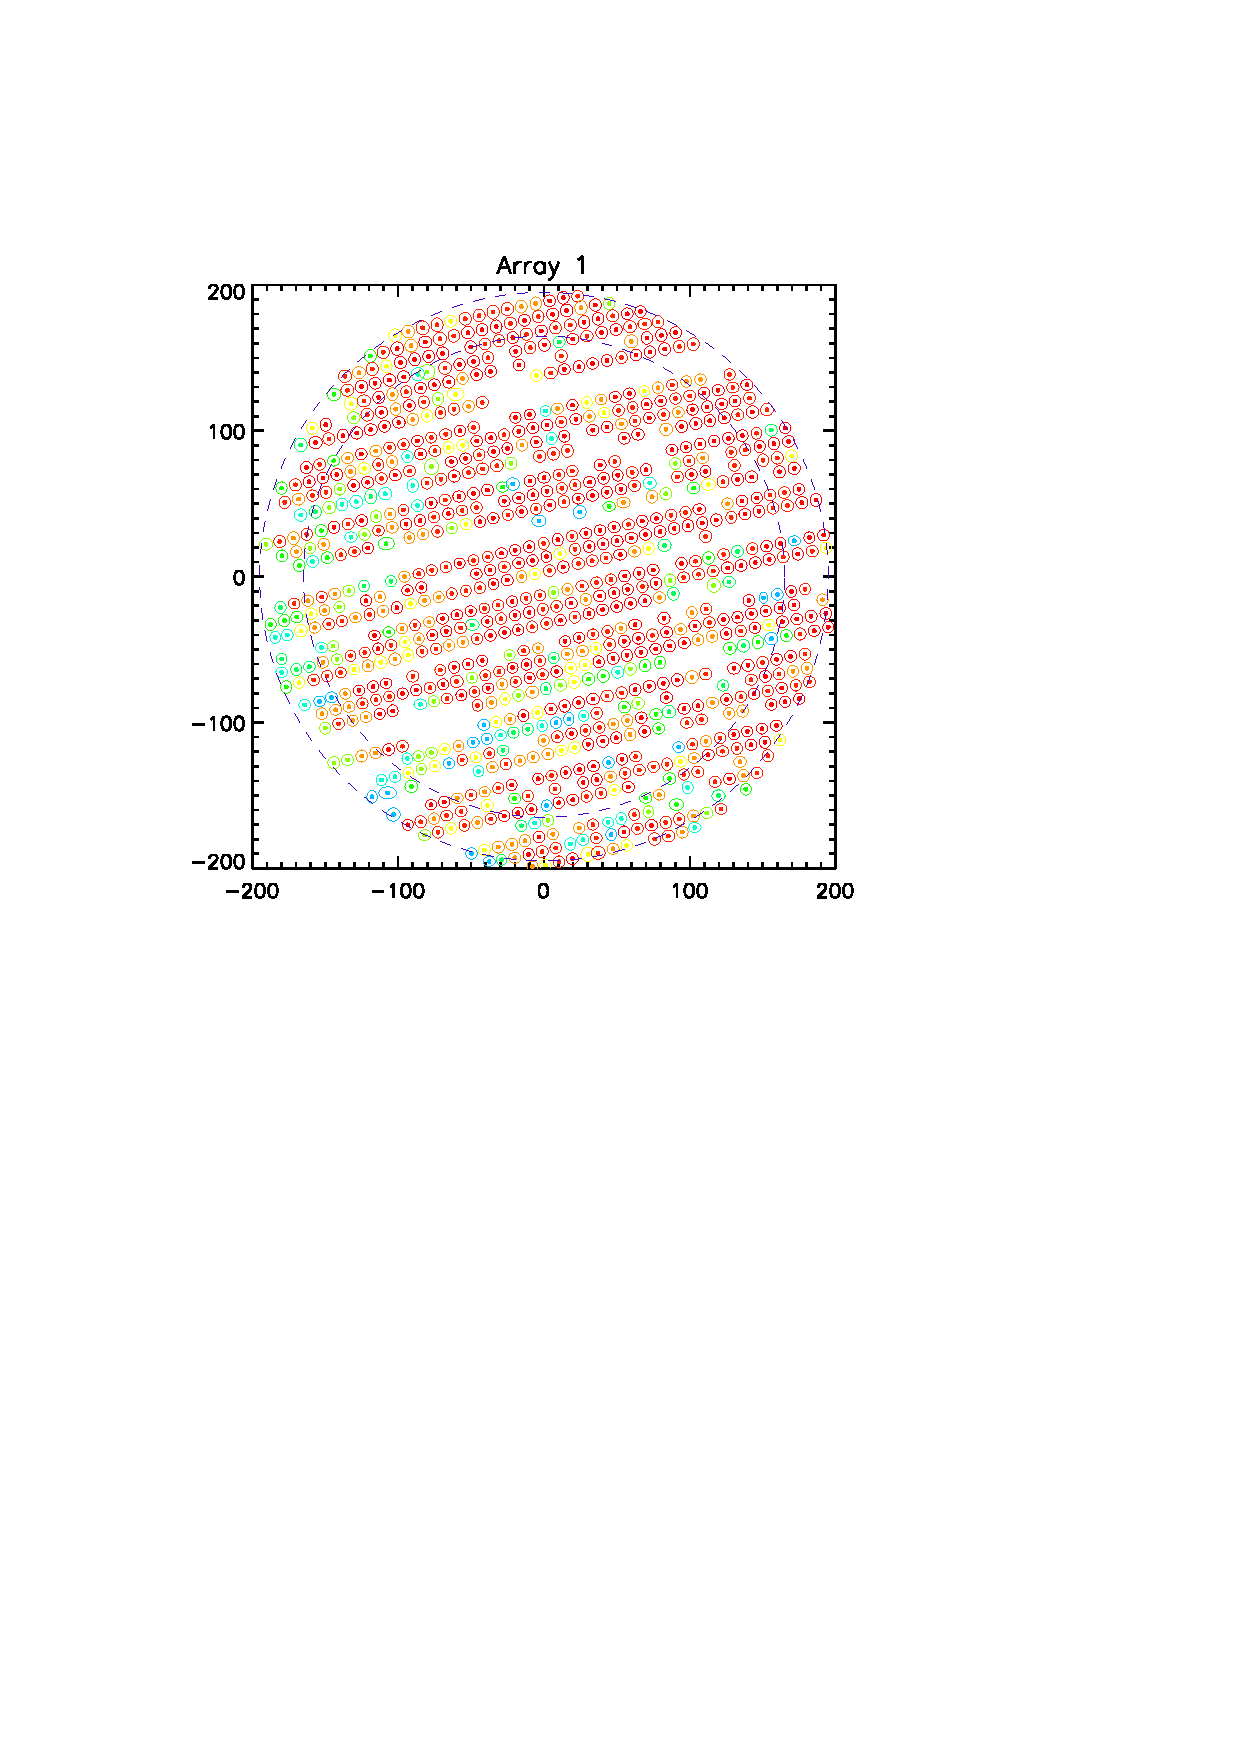
\includegraphics[trim=3cm 14cm 6cm 4cm, clip=true, width=0.32\linewidth]{Figures/A1_fwhm_color_count.pdf}
%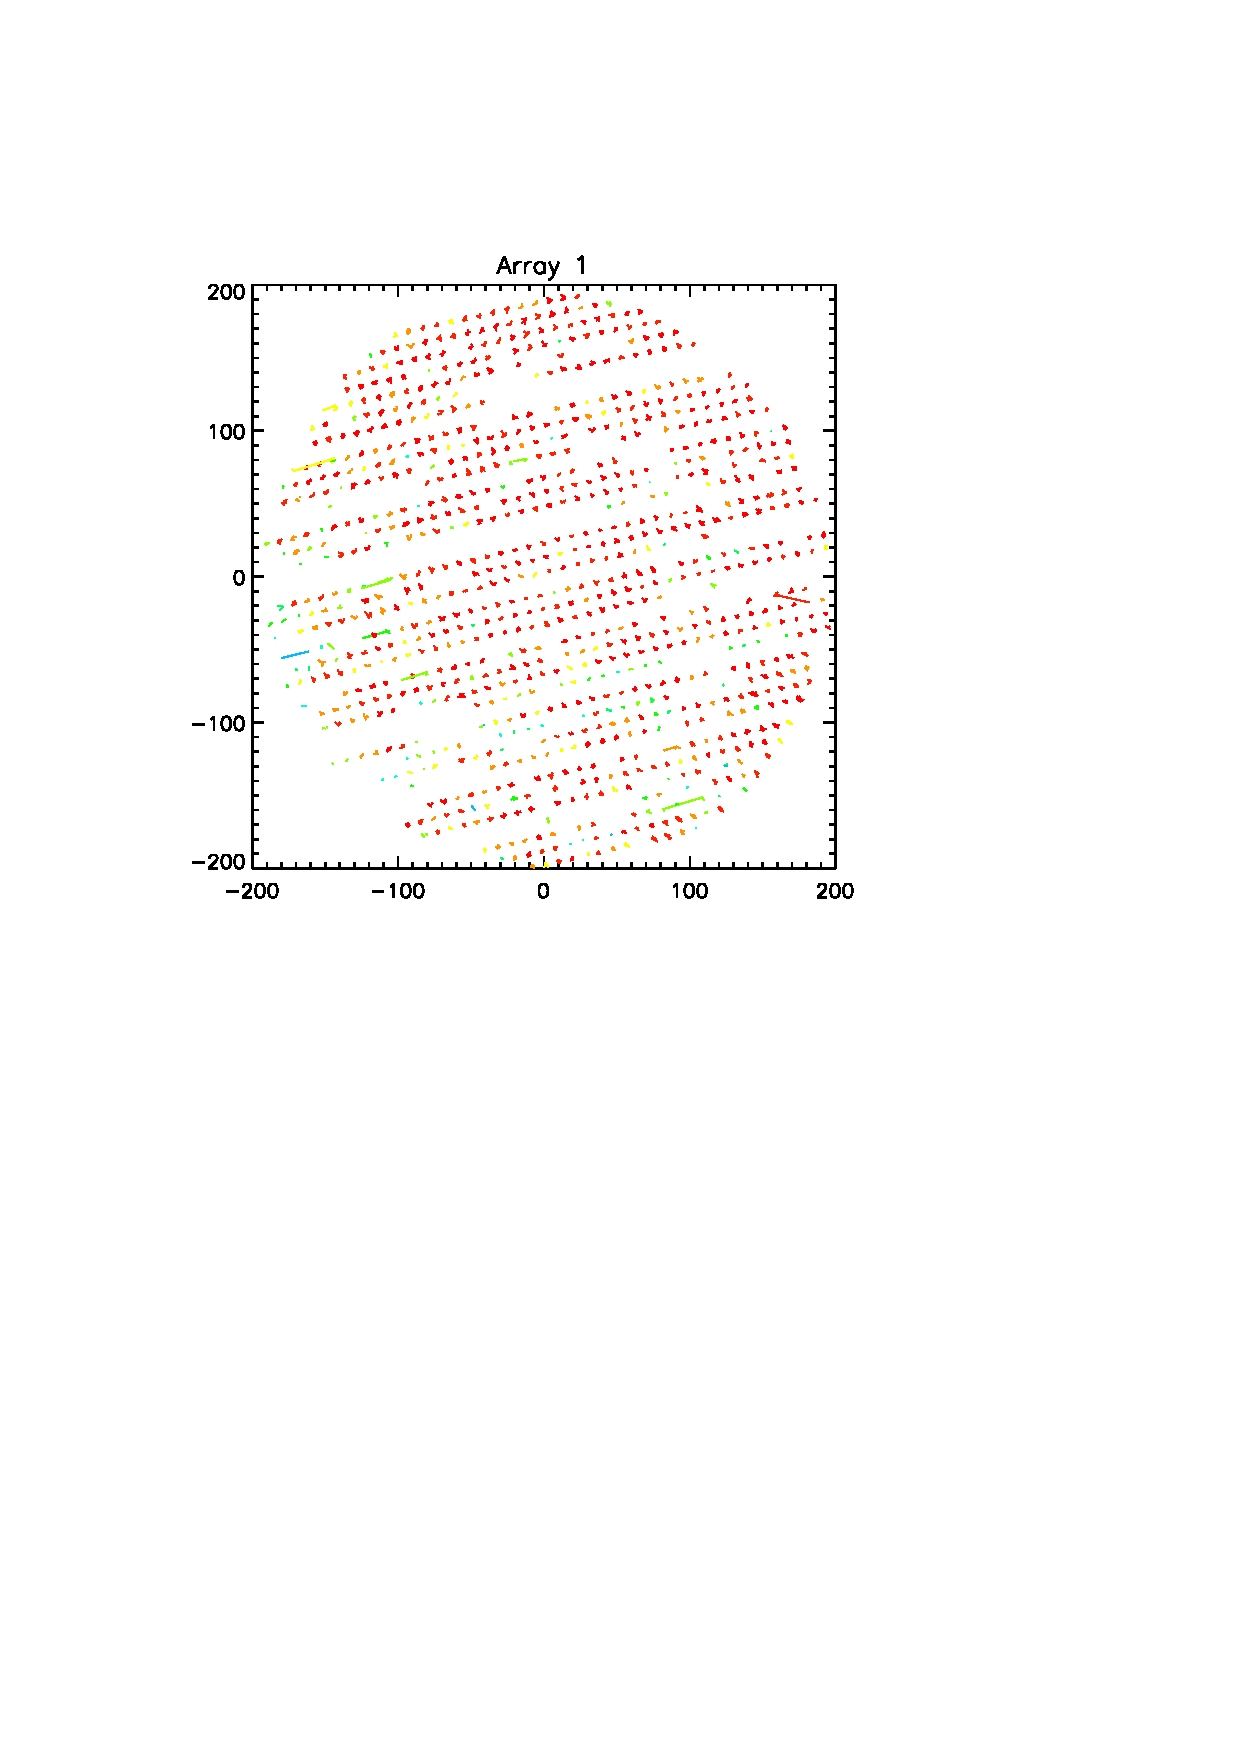
\includegraphics[trim=2cm 14cm 5cm 4cm, clip=true,width=0.45\linewidth]{Figures/A1_positions.pdf}
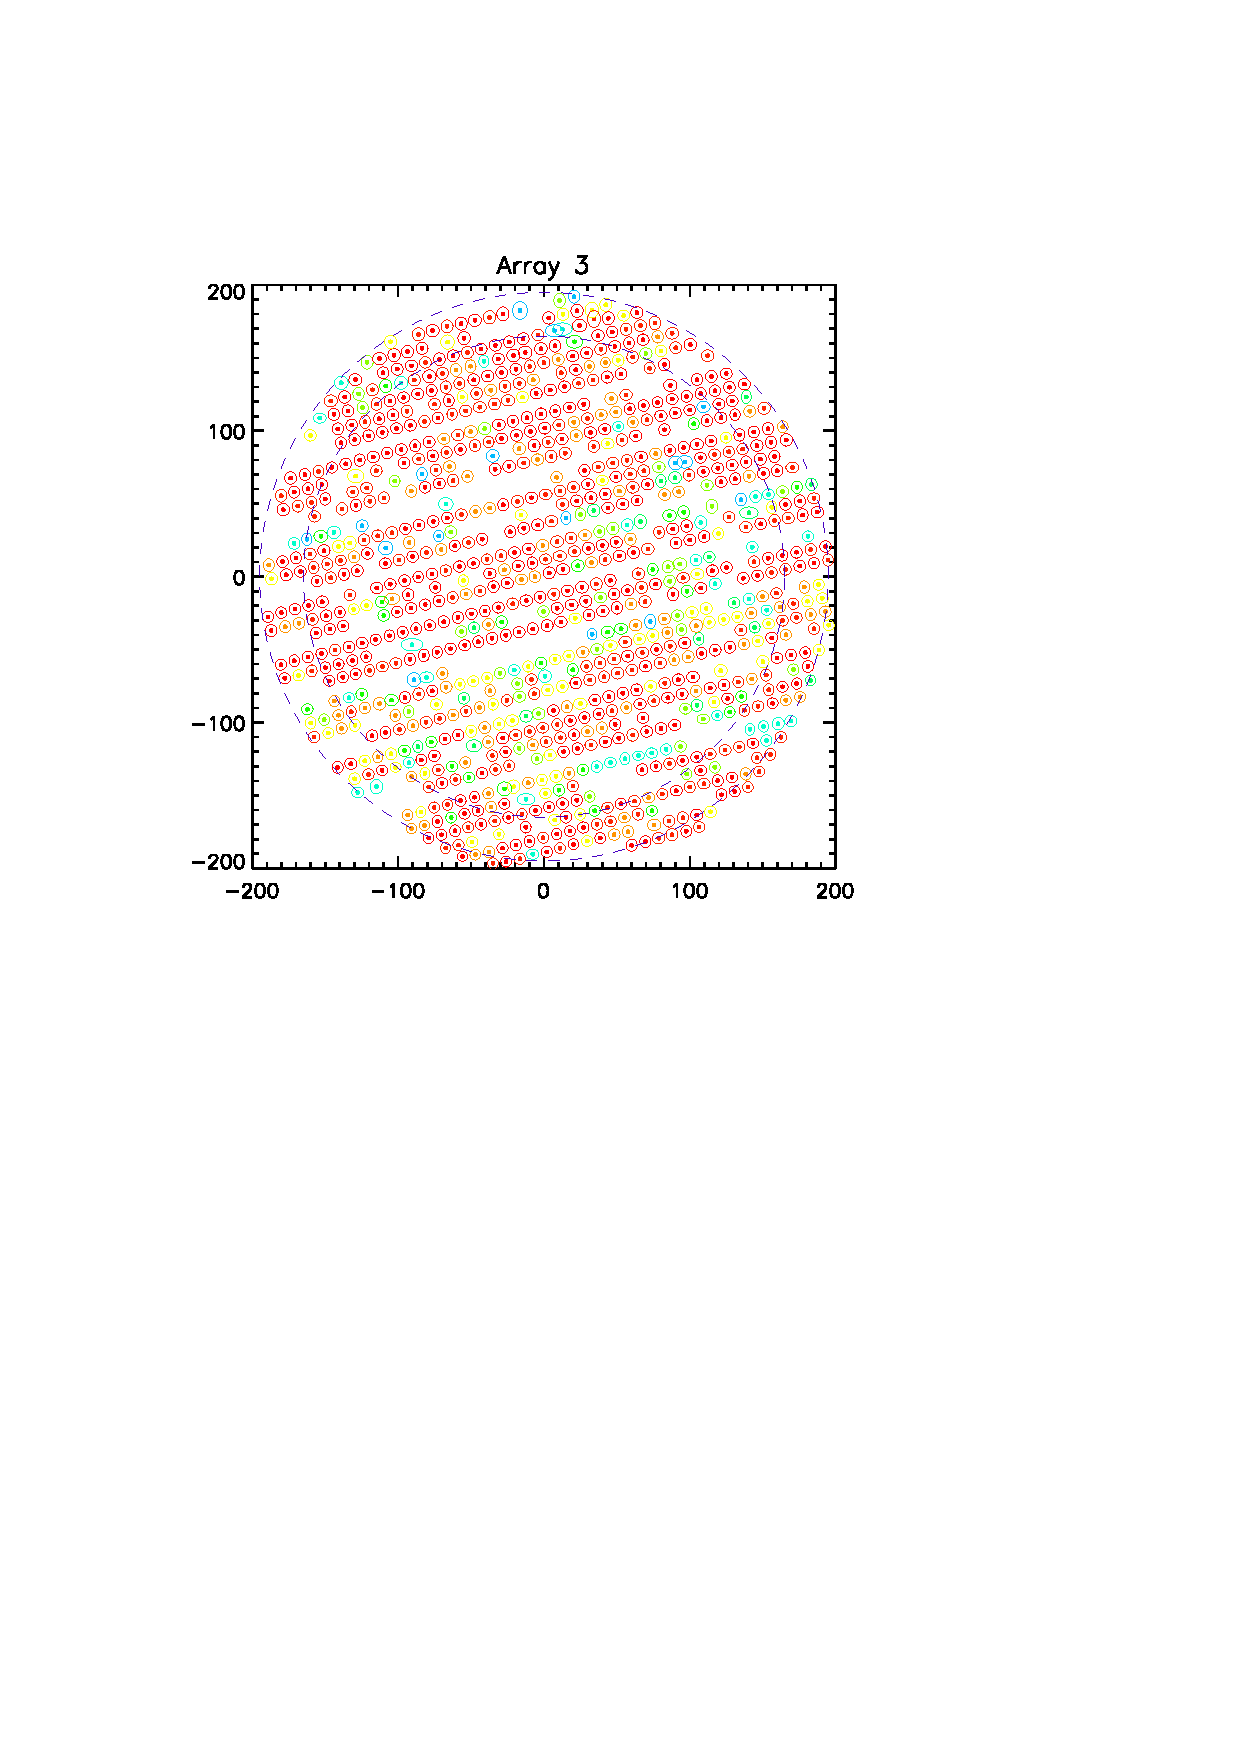
\includegraphics[trim=3cm 14cm 6cm 4cm, clip=true, width=0.32\linewidth]{Figures/A3_fwhm_color_count.pdf}
%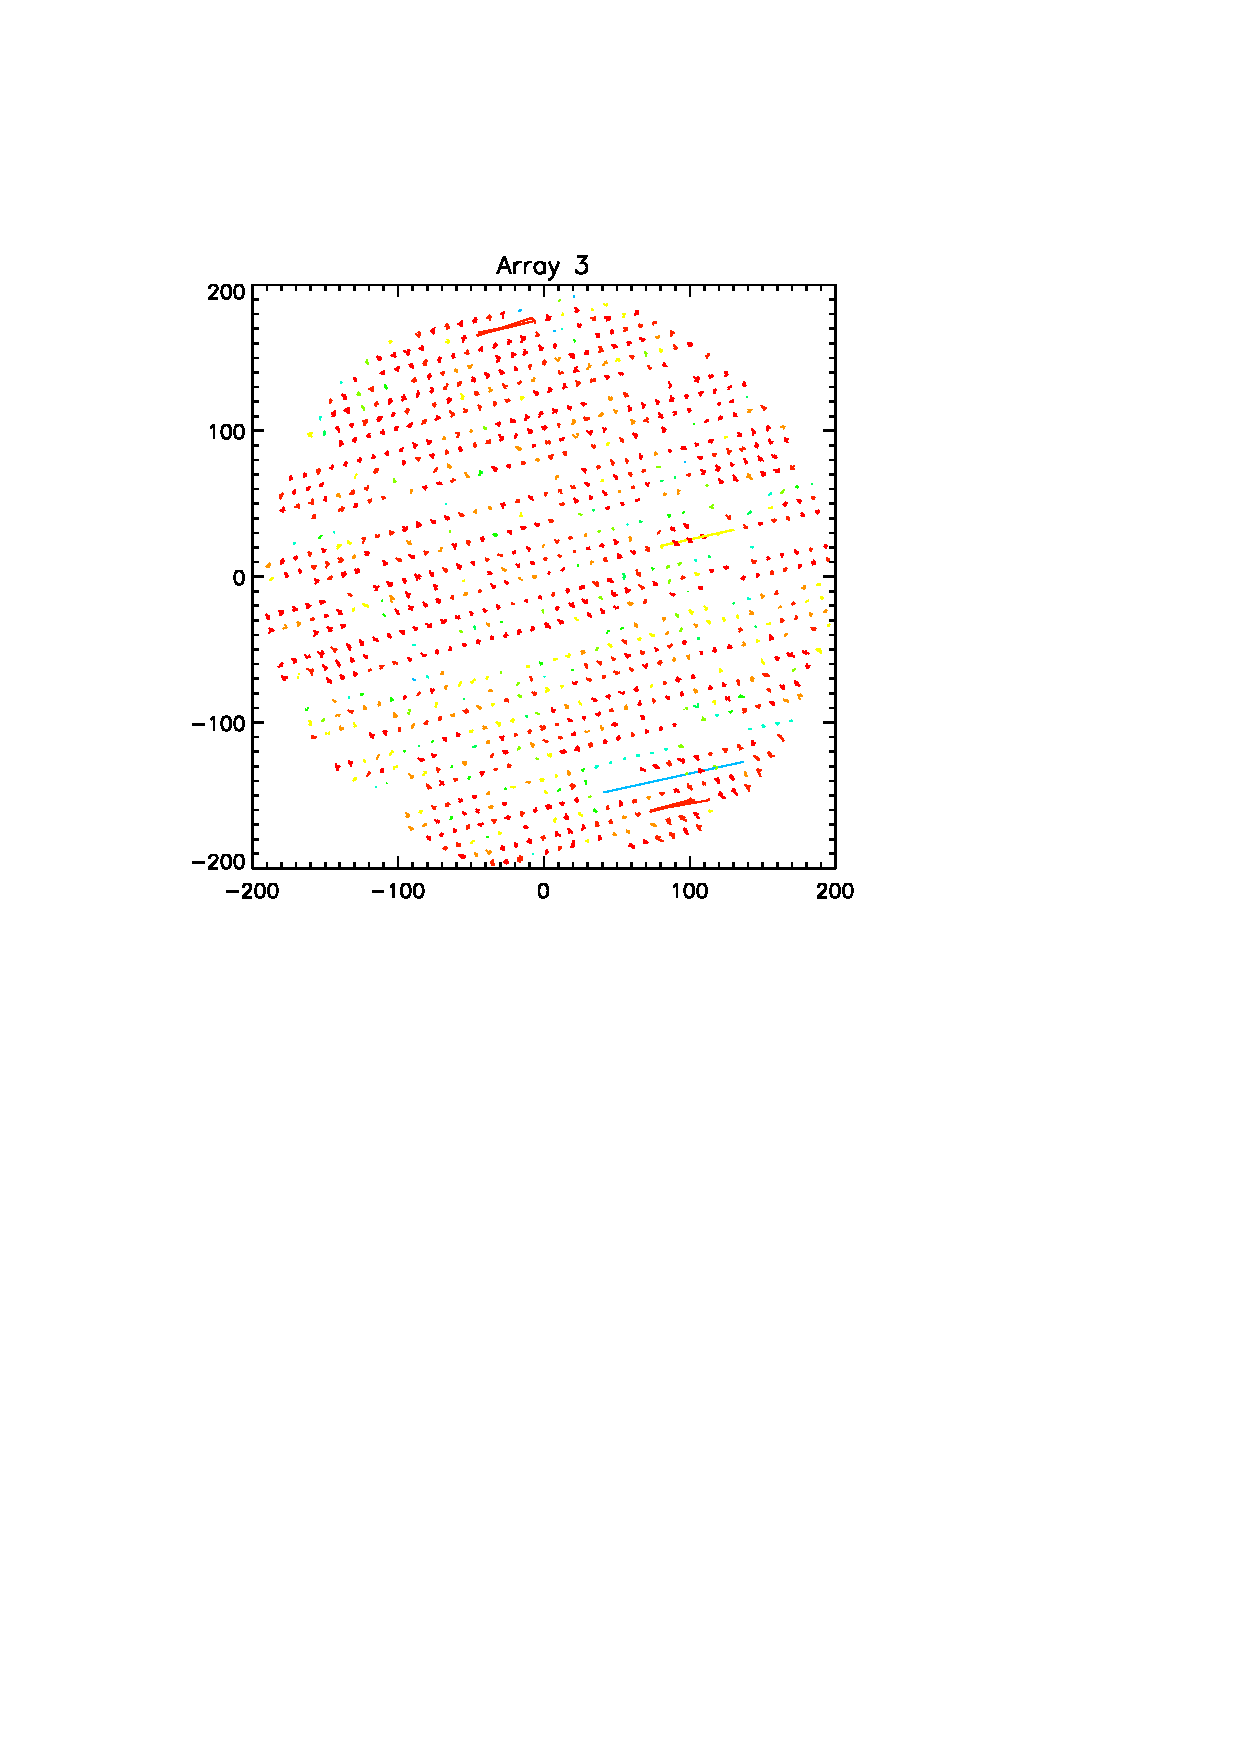
\includegraphics[trim=2cm 14cm 5cm 4cm, clip=true,width=0.45\linewidth]{Figures/A3_positions.pdf}
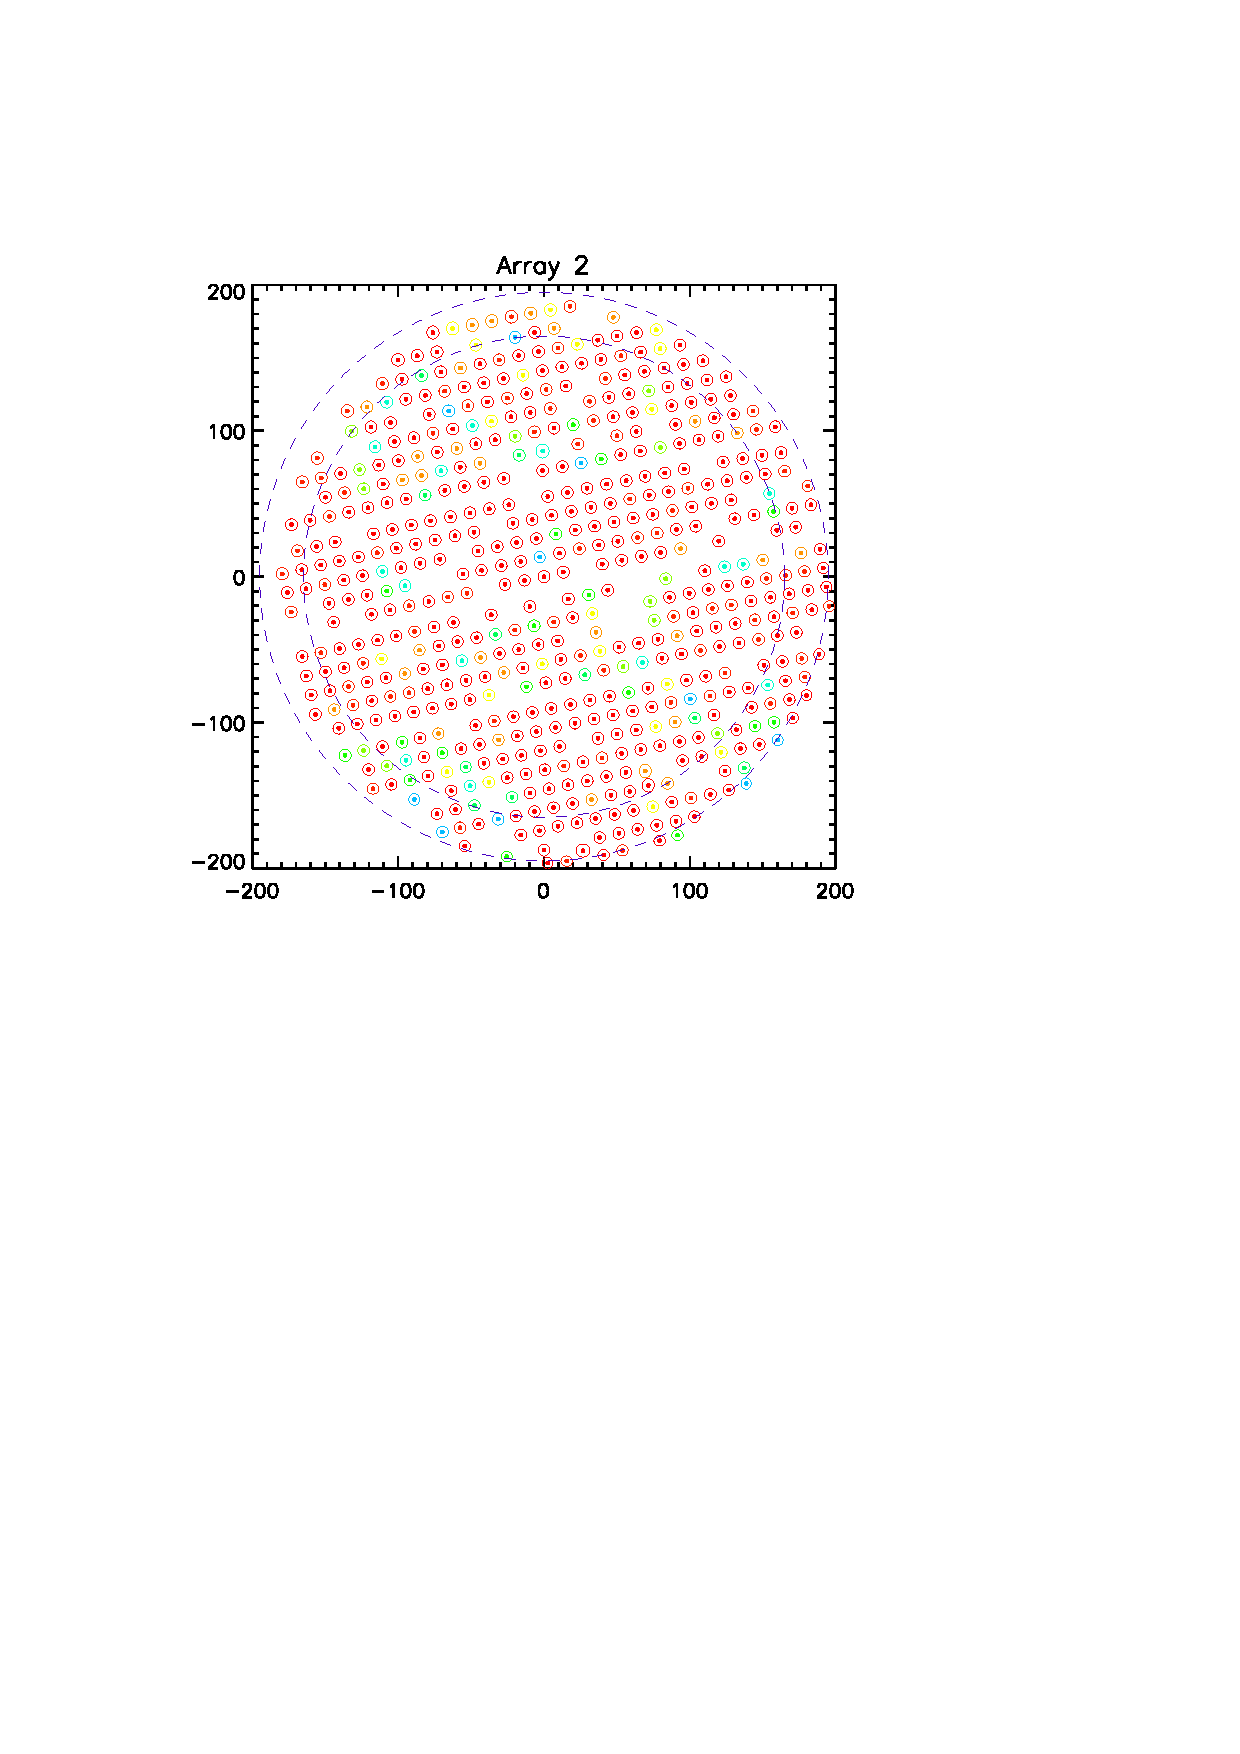
\includegraphics[trim=3cm 14cm 6cm 4cm, clip=true, width=0.32\linewidth]{Figures/A2_fwhm_color_count.pdf}
%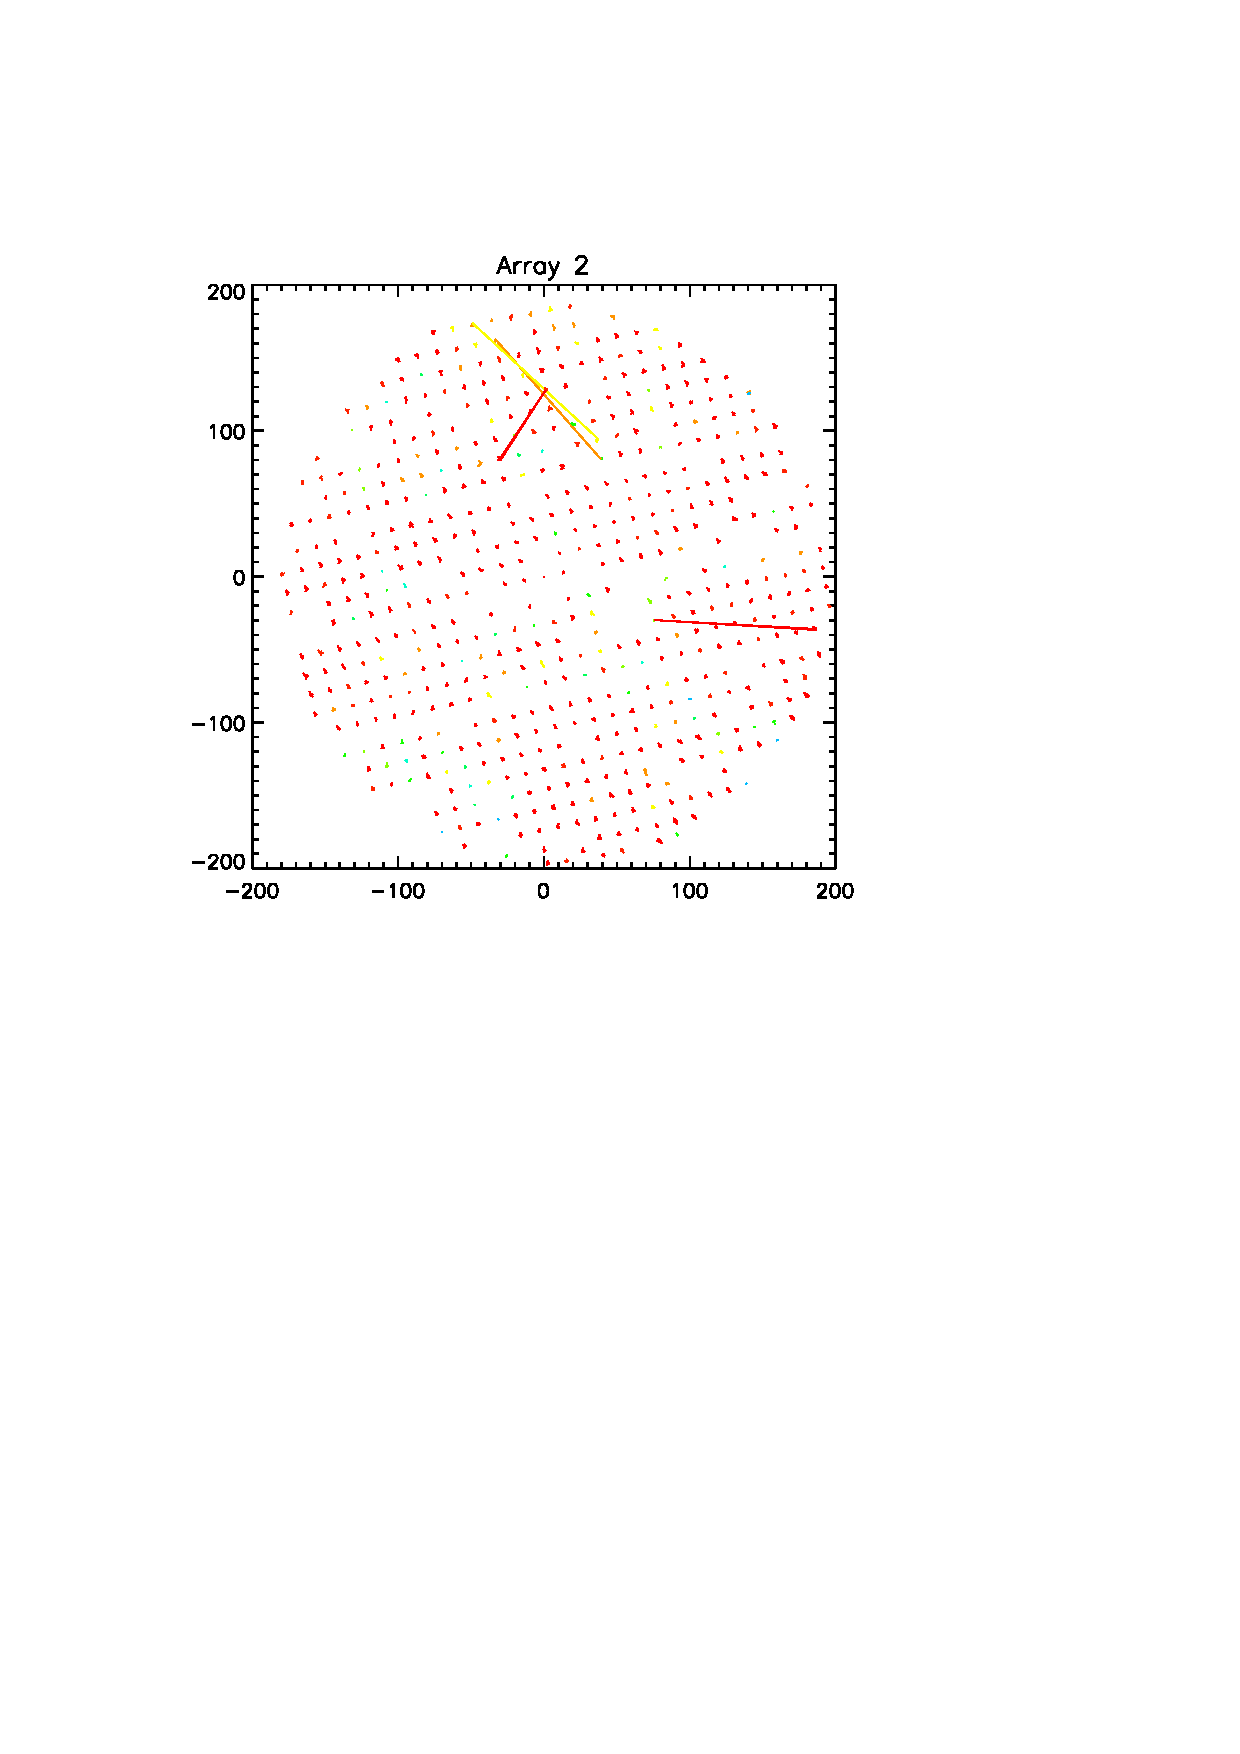
\includegraphics[trim=2cm 14cm 5cm 4cm, clip=true,width=0.45\linewidth]{Figures/A2_positions.pdf}
\caption[KID selection in the FOV]{Average detector positions
  for arrays A1, A3, and A2. The three plots show the detectors that
  met the quality criteria for at least two \bms\ during two technical
  campaigns: 952, 961, and 553 for A1, A3 and A2, respectively. The color
  indicates, from green to red, how many times a KID was
  identified as valid on a \bm. The inner and outer
  dash-line circles correspond to a FOV of 5.5\,arcmin and 6.5\,arcmin,
  respectively. Units are arcseconds.}
\label{fig:avg_fov_color}
\end{center}
\end{figure*}

\subsection{FOV grid distortion}
\label{se:grid_distortion}

We compare the reconstructed KID positions in the FOV to their design
positions in the array. We fit the 2D field translation and rotation that allow
matching the measured KID positions with the design positions using a 2D
polynomial mapping function. {\lp We find that a matching can be
obtained using a 2D polynome of degree one, that is using a linear
shift and a rotation only.} We call distortion cross-terms
between the two spatial coordinates in the polynomial fit.

The aim is twofold. First we obtain a detailed
characterisation of the real geometry of NIKA2 focal plane. Secondly,
this analysis constitutes the last step of the KID
selection, and the most deviant KIDs, whose measured position deviates
by more than $4''$ from the design position are discarded. 

We present the global results of the grid distortion
analysis using the KID positions given
by the focal plane geometry procedure, as described in
Sect.~\ref{se:fov_geometry}, applied to a \bm\ scan acquired
during the first scientific campaign (\aka\ N2R12). 
%Note that the
%selected KID numbers are low
%in this example as the scans were acquired during the daytime
%and suffers from temperature-induced instabilities (see
%Sect.~\ref{se:beam_variation}).
%We performed two tests. One test is based on using all the designed
%KIDs, while the second test relies on a KID selection applied in the
%FOV geometry obtained from the \bm\ scan. The KID selection, which
%consists in discarding the KIDs the most impacted by the cross-talk
%effect or the {\tt tuning} failures, is detailed in
%Sect.~\ref{se:avg_kidpar}.
The initial
number of KID considered in this analysis results from
a first KID selection, which consists in discarding the KIDs that are the most
impacted by the cross-talk effect or the {\tt tuning} failures,
applied in the FOV geometry obtained from the \bm\ scan. More details
on the KID selection are given in the next section. %Sect.~\ref{se:avg_kidpar}.
The results are gathered in Table~\ref{ta:gridmatch}.

\begin{table}[!htbp]
  \caption[Field-of-view deformations]{Field-of-view
  deformation. Example of mapping of the observed KID positions in the
  sky to their mechanically designed positions. The initial table of
  selected KIDs is given by the focal plane geometry procedure, as
  described in Sect.~\ref{se:fov_geometry}, applied to a \bm\ scan
  acquired during the N2R12 campaign. %Note that the selected KID numbers are particularly
    %low in this example, as the scans were observed during the daytime
    %and suffer from temperature-induced instabilities (see
    %Sect.~\ref{se:beam_variation}). Even in this pessimistic case,
    More than 90\% of the detectors are within less than 5 arcseconds
    of their expected position.}
  \label{ta:gridmatch}
  \centering
  \begin{tabular}{r|c|c|c}
    \hline
    \hline
    Characteristic &  Array 1  &	Array 3   &	Array 2  \\
    \hline
    \small{$\lambda$ [mm]}  &  1.25     &      1.25      &    2.05   \\
    %\small{Designed KID}                     & 1140  &  1140 & 616  \\
    %\small{Well-placed KID}                  &  864  &  808  & 488  \\
    \small{Selected KID}\tablefootmark{a}    &  866  &  808  & 488  \\
    \small{Well-placed KID}         &  864  &  808  & 488  \\
    %\small{Ratio [\%]}\tablefootmark{b}      &  76   &  71   & 79   \\
    %&673/736  &	734/758   &    437/444   & \small{Well-placed KIDs (WPK)/Found KIDs (FK)} \\
    %&91/59 	 &      96/64 	  &    98/71 	 & \small{Ratio [\%] of WPK/FK and WPK/TDK} \\
    \small{Median deviation\tablefootmark{b}  [arcsec]}    & 1.01    &     0.95   &    0.75  \\
    \small{Mean distortion\tablefootmark{c} [arcsec]}                       & 1.09    &     1.01   &    0.84  \\
    \small{Array center\tablefootmark{d} [arcsec]}  & (1.9, -5.1) & (2.3, -6.2) &  (9.6, -7.8) \\
    \small{Scaling\tablefootmark{e} [arcsec/mm]}   &  4.9     &	4.9      &    4.9 \\
    %& \small{Plate scaling [arcsec/mm] in the Design x and y (averaged)} \\
    \small{Rotation angle\tablefootmark{f} [degree]} & 77.3     &	76.3      &    78.2  \\
    %\small{FOV [arcmin] (Total KIDs)}                      & 6.6      &	6.6       &    6.6   \\
    \small{Grid step\tablefootmark{g} [arcsec, mm] }     & 9.8, 2.00 &	9.7, 2.00  &    13.3, 2.75 \\
    % Old values, rechecked (difference comes from lambda and D)
    %   1.24  &	1.22  &	0.97  &	Distance between near detectors with $30\,\rm{m}$ diameter aperture [in $\lambda$/D] \\
    % here new values checked FXD 30 Nov 2018 1.11 1.10 0.87
    \small{Grid step\tablefootmark{h} [$\lambda$/D] } & 1.11     &	1.10      &	0.87  \\
    %\new{with $27\,\rm{m}$ effective diameter aperture} [in $\lambda$/D]} \\
    \small{Modeled grid step\tablefootmark{i} [$\lambda$/D]}  & 1.09     &      1.09      & 0.93    \\
    \hline
  \end{tabular}
  \tablefoot{ \\
    %\tablefoottext{a}{Initial number of KIDs given in a FOV geometry
    %  for the N2R9 campaign (pessimistic case)}
    \tablefoottext{a}{Initial number of KIDs selected in a FOV geometry using a \bm\ scan of the N2R12 campaign}
    %\tablefoottext{b}{Ratio of the well-placed KID to the designed KID numbers}      
    \tablefoottext{b}{Median distance [arcsec] between the design position and the measured position of the KIDs}
    \tablefoottext{c}{{\lp Average best-fit cross term of the polynomial model across the FOV [arcsec]}}
    \tablefoottext{d}{Array center in Nasmyth coordinates}
    \tablefoottext{e}{Averaged scaling between the measured grid and the designed grid}
    \tablefoottext{f}{Rotation from the design to Nasmyth coordinates}
    \tablefoottext{g}{Distance between neighbour detectors}
    \tablefoottext{h}{Distance between neighbour detectors using the
  reference frequencies ($260\,\rm{GHz}$ and $150\,\rm{GHz}$) and a
  27\,m effective diameter telescope aperture (see Sect.~\ref{se:instru_optics})}
    \tablefoottext{i}{Distance between neighbour detectors modeled using ZEMAX simulation}
  }
\end{table}

Most of the selected KID are also well-placed, that is at less than 4'' from
their expected position. Moreover, on average the position of each
detector is known to about one arcsecond. We find
that Array 1 has some of the most deviant detectors (above 4''
from their expected position). These detectors are excluded from
further analysis. The two 1\,mm arrays have almost
the same center but this center differs by $7''$ and $2''$ in the two Nasmyth
coordinates, respectively, from the 2\,mm array center. This has no impact on the
pointing nor the focus settings. The sampling is above $\lambda/D$ at
1\,mm, assuming a 27\,m effective diameter aperture. Note that
the rotation angle between the array and the Nasmyth
coordinates was designed as 76.2\,degrees, less than 2 degrees from
what is observed.


These results have been compared to expectations obtained using ZEMAX
simulation. 
%The grid diagram generated using ZEMAX provides us with
%the maximum dispersion in the field defined by
%
%\begin{equation}
%P = \frac{\sqrt{(x_p - x_r)^2 + (y_p - y_r)^2}}{\sqrt{x_p^2 + y_p^2}},
%\end{equation}
%
%where $(x_p, y_p)$ and $(x_r, y_r)$ are respectivelly the predicted
%and real coordinates on the image surface relative to the reference
%field position image location (see page 170 of the ZEMAX manual, 2007).
%The predicted coordinates for the whole field are obtained using a
%linear interpolation of a small area in the field central part,
%whereas the real coordinates are calculated by ray tracing through the
%optical system.
%
%\begin{figure}[ht] 
%\begin{center}
%  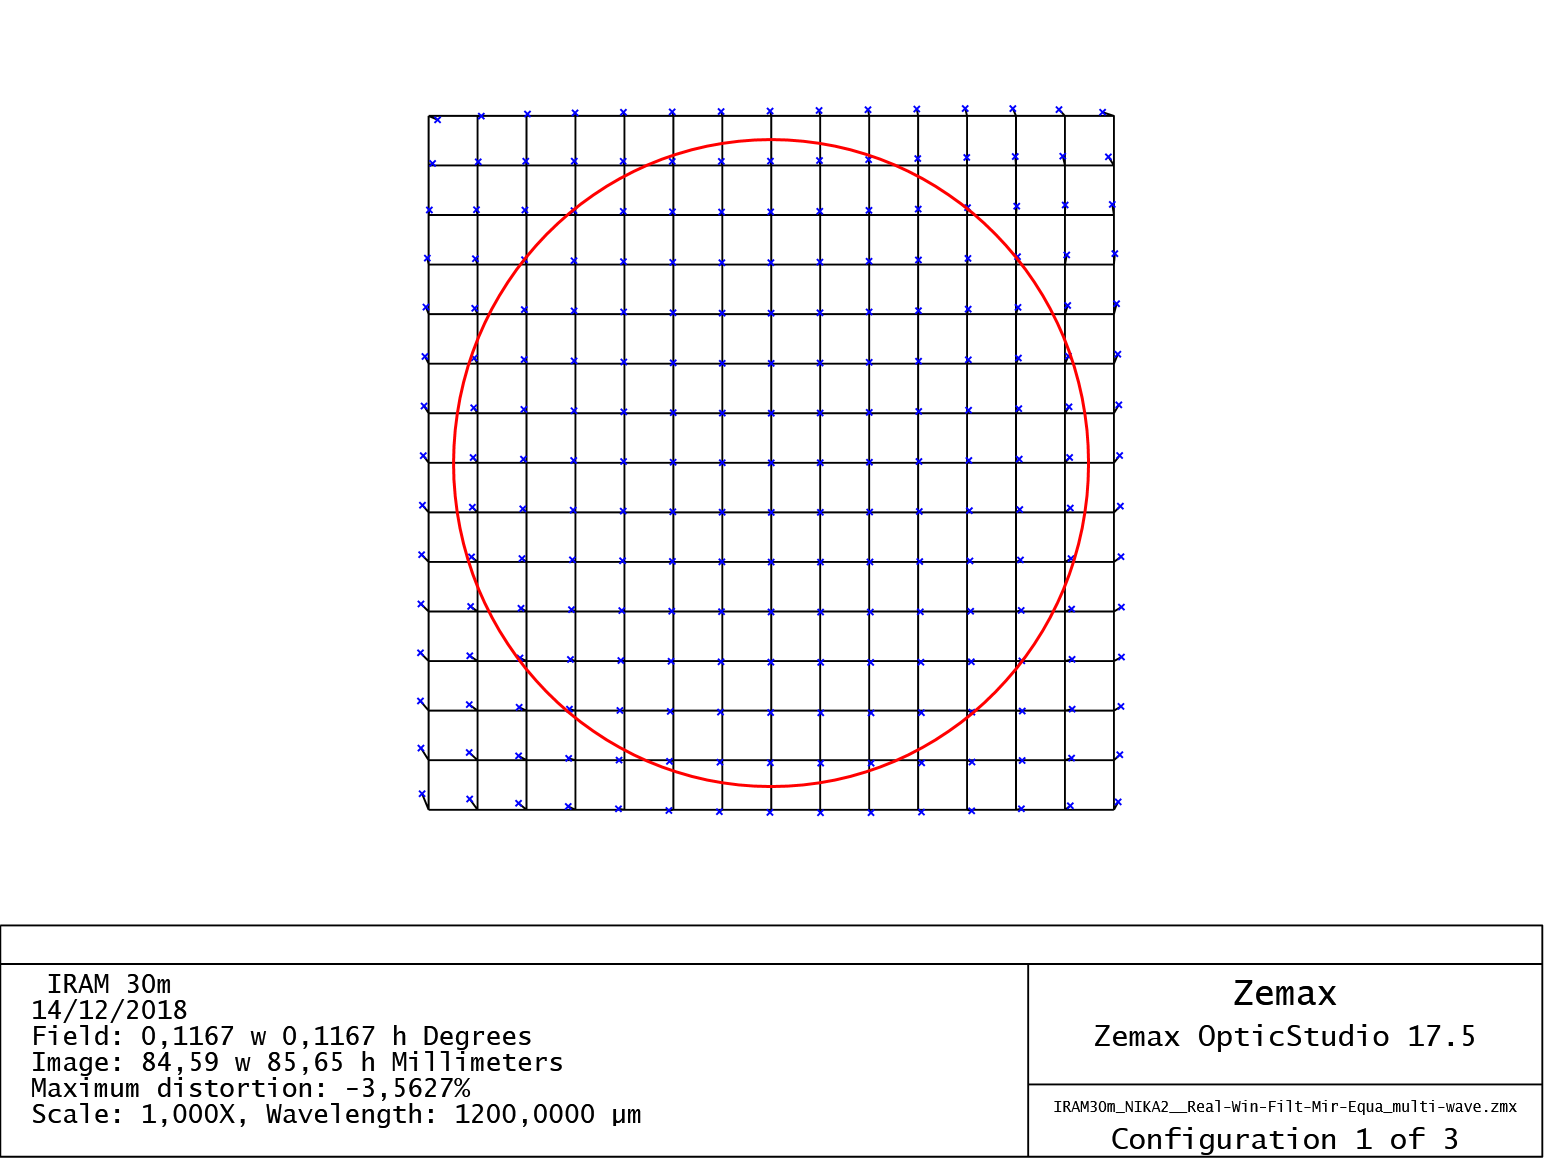
\includegraphics[width=0.9\textwidth]{Figures/NIKA2_Grid-distortion.png}
%  \caption[Simulated FOV grid]{NIKA2 grid diagram simulated using
%    ZEMAX. \new{The step of the grid is of 30 arcsec and the side width
%      of the black square is of seven arcmin. The red circle corresponds to the 
%      $6.5\,\rm{arcmin}$ diameter FOV. Blue crosses show the grid
%      distorsions in az-el coordinates and in the case of an observing
%      elevation of $14^o$. These grid distorsions depends on the
%      telescope elevation, whereas in the image plane (the plane of the
%      KID arrays) the distorsions are invariant. This allows for
%      concluding that the grid distorsions are caused by the optical
%      elements located between M4 and the dichroic plate.} 
%  }
% \label{fig:fov_grid_distortion_zemax}
%\end{center}
%\end{figure}
%Figure \ref{fig:fov_grid_distortion_zemax} shows the ZEMAX grid diagram for
%NIKA2 simulated optic system.
%
We generated a grid diagram for the NIKA2 optical system and found a maximum
grid distortion of $2.7\%$ in the $6.5'$ FOV. We notice that the
strongest distortion appear in the upper right corner of the Nasmyth plan, which is
also the area of the largest defocus w.r.t. to the center (see
Sect.~\ref{sec:focus_surfaces}).
An expected distortion of $2.7\%$ is at most a 5'' shift from the
center to the outside of the array. The quoted distortions between the
measured and design positions are well within the expected
maximum distortions from the NIKA2 optics.

%Auxillary information on this work can be found in this wiki post\footnote{\tiny
%  {\tt http$://$www.iram.fr$/$wiki$/$nika2$/$index.php$/$April$\_$19,$\_$2017,$\_$FXD,$\_$KID$\_$position$\_$mapping$\_$and$\_$Field$\_$distortion$\_$for$\_$Run9}}.
% FXD: this would need to be more ascertained. Lack of time to go further.


\subsection{KID selection and average geometry}
\label{se:avg_kidpar}

In order to identify the most stable KIDs, we compare the KID parameters
obtained using several \bms.  In the following, we show results as
obtained using seven \bms\ acquired during two technical observation
campaigns in 2017.
%from Run10, two from Run9 and one from Run8.
For each KID we
compute the average position on the focal plane and the average FWHM, counting
the times that it has been considered as valid and at the same position. 
A few KIDs have very close resonance frequencies and can be misidentified on some scans. A
few others must also be discarded because they appear identical numerically due
to the fact that a same (noisy) KID can sometimes be associated
to two different frequency tones in the acquisition system.
These KIDs are flagged out (less than 1\% of the design KIDs).

In Fig.~\ref{fig:avg_fov_color} we show the
average focal plane reconstruction. The colors, from green to red,
represent the number of times that the KID has been considered as valid.
The eight feed lines for each of the two
$1\,\rm{mm}$ arrays are also visible in this figure. First, slightly
larger spaces are seen between KID rows connected to different
feed lines than between KID rows of the same feed line. Second,
KIDs at the end of a feed line are less often valid than the others
(see e.g. the FOV of Array 3). As the tone frequencies
increase with the KID position in the feedline, some KIDs are
sometimes missing because their frequency lays above the maximum tone
frequency authorized by the readout electronics. That explains the linear holes
in the middle of the $1\,\rm{mm}$ arrays. For A1, this end-of-feedline
effect is mixed with the effect of the KID gain variation across the
FOV, which mainly affects the lower left third of the array, as
discussed in Sect.~\ref{se:flat_field}.

For A1, A3 and A2, respectively, we have 952, 961, and 553 KIDs that
have been considered as valid at least twice. From this, we deduce the fraction of
valid detectors over the design ones, as given in Table~\ref{tab:number_of_kids}.

%% \begin{figure}[htp]
%% \begin{center}
%% 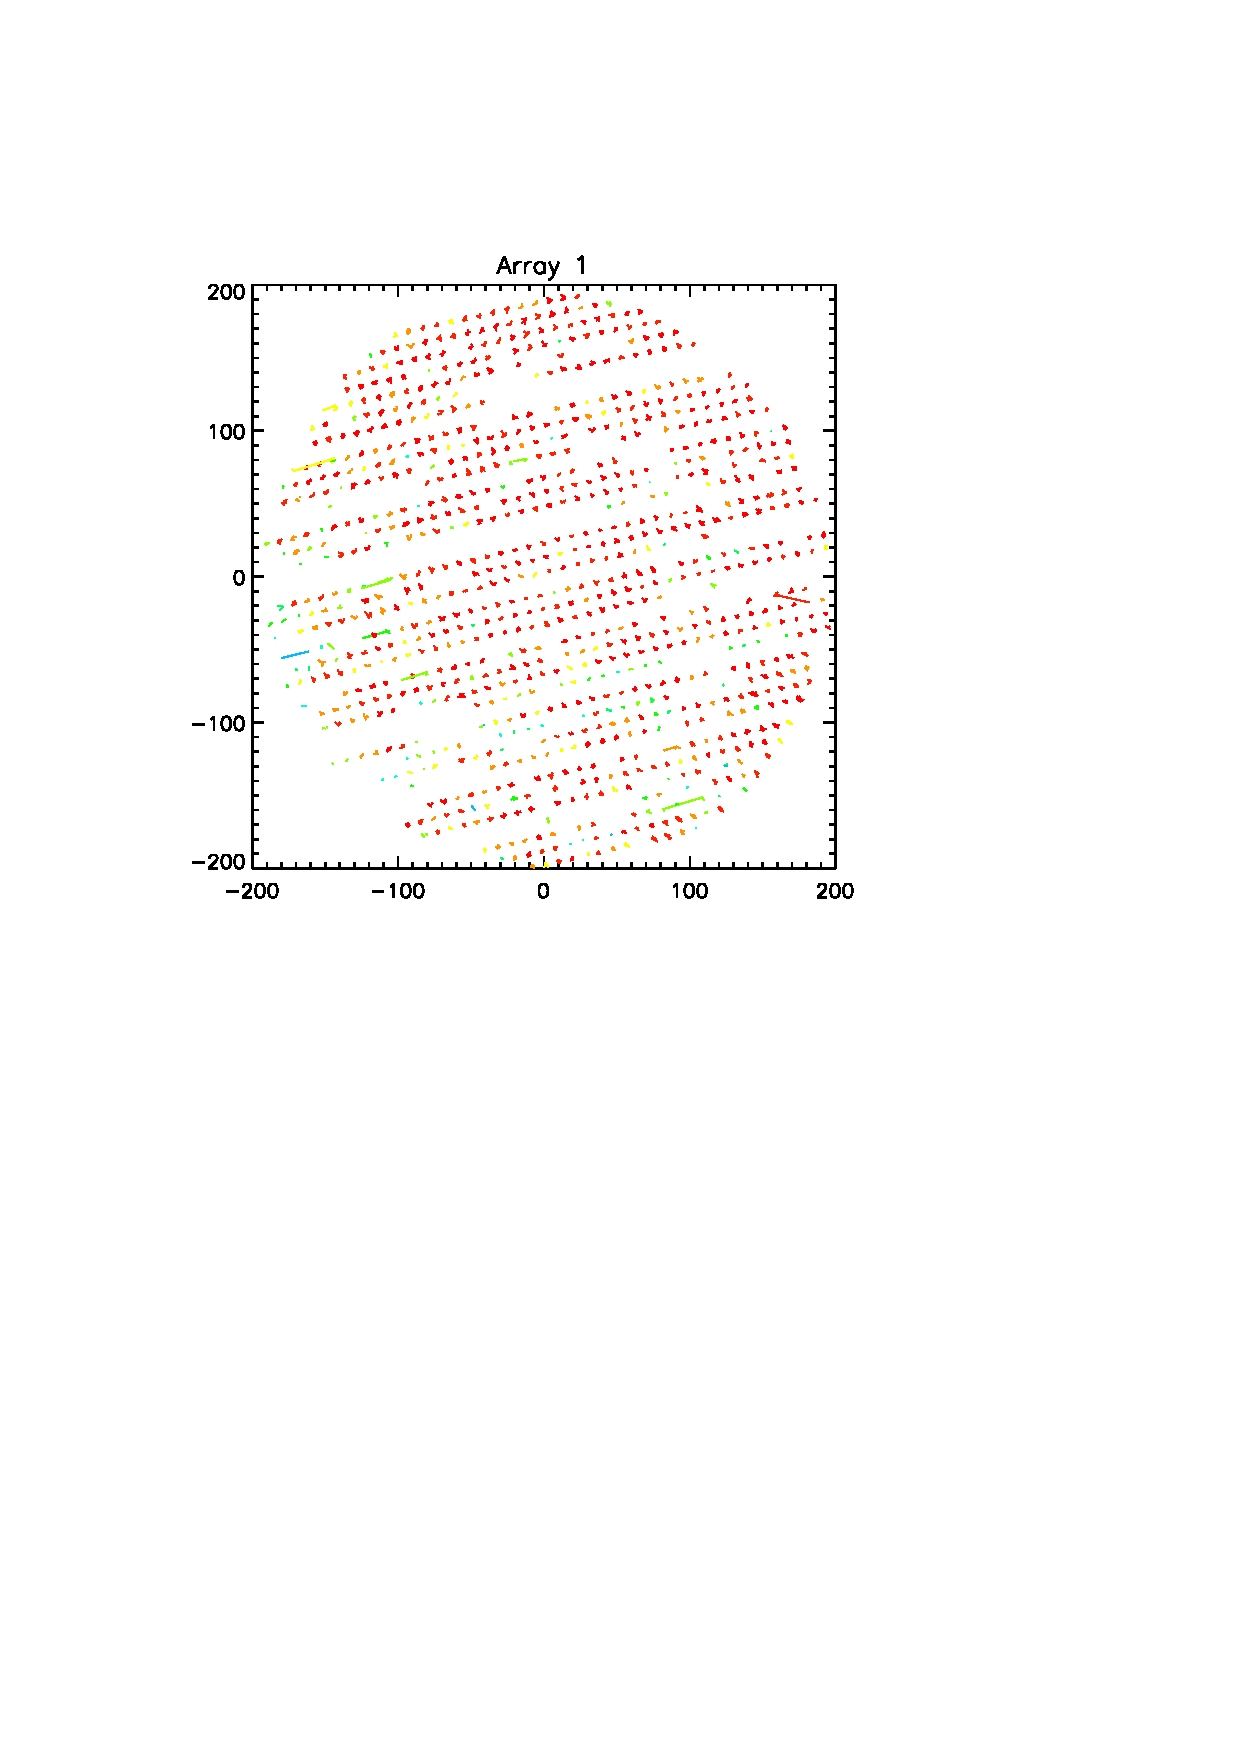
\includegraphics[trim=2cm 14cm 5cm 4cm, clip=true,width=0.55\linewidth]{Figures/A1_positions.pdf}
%% 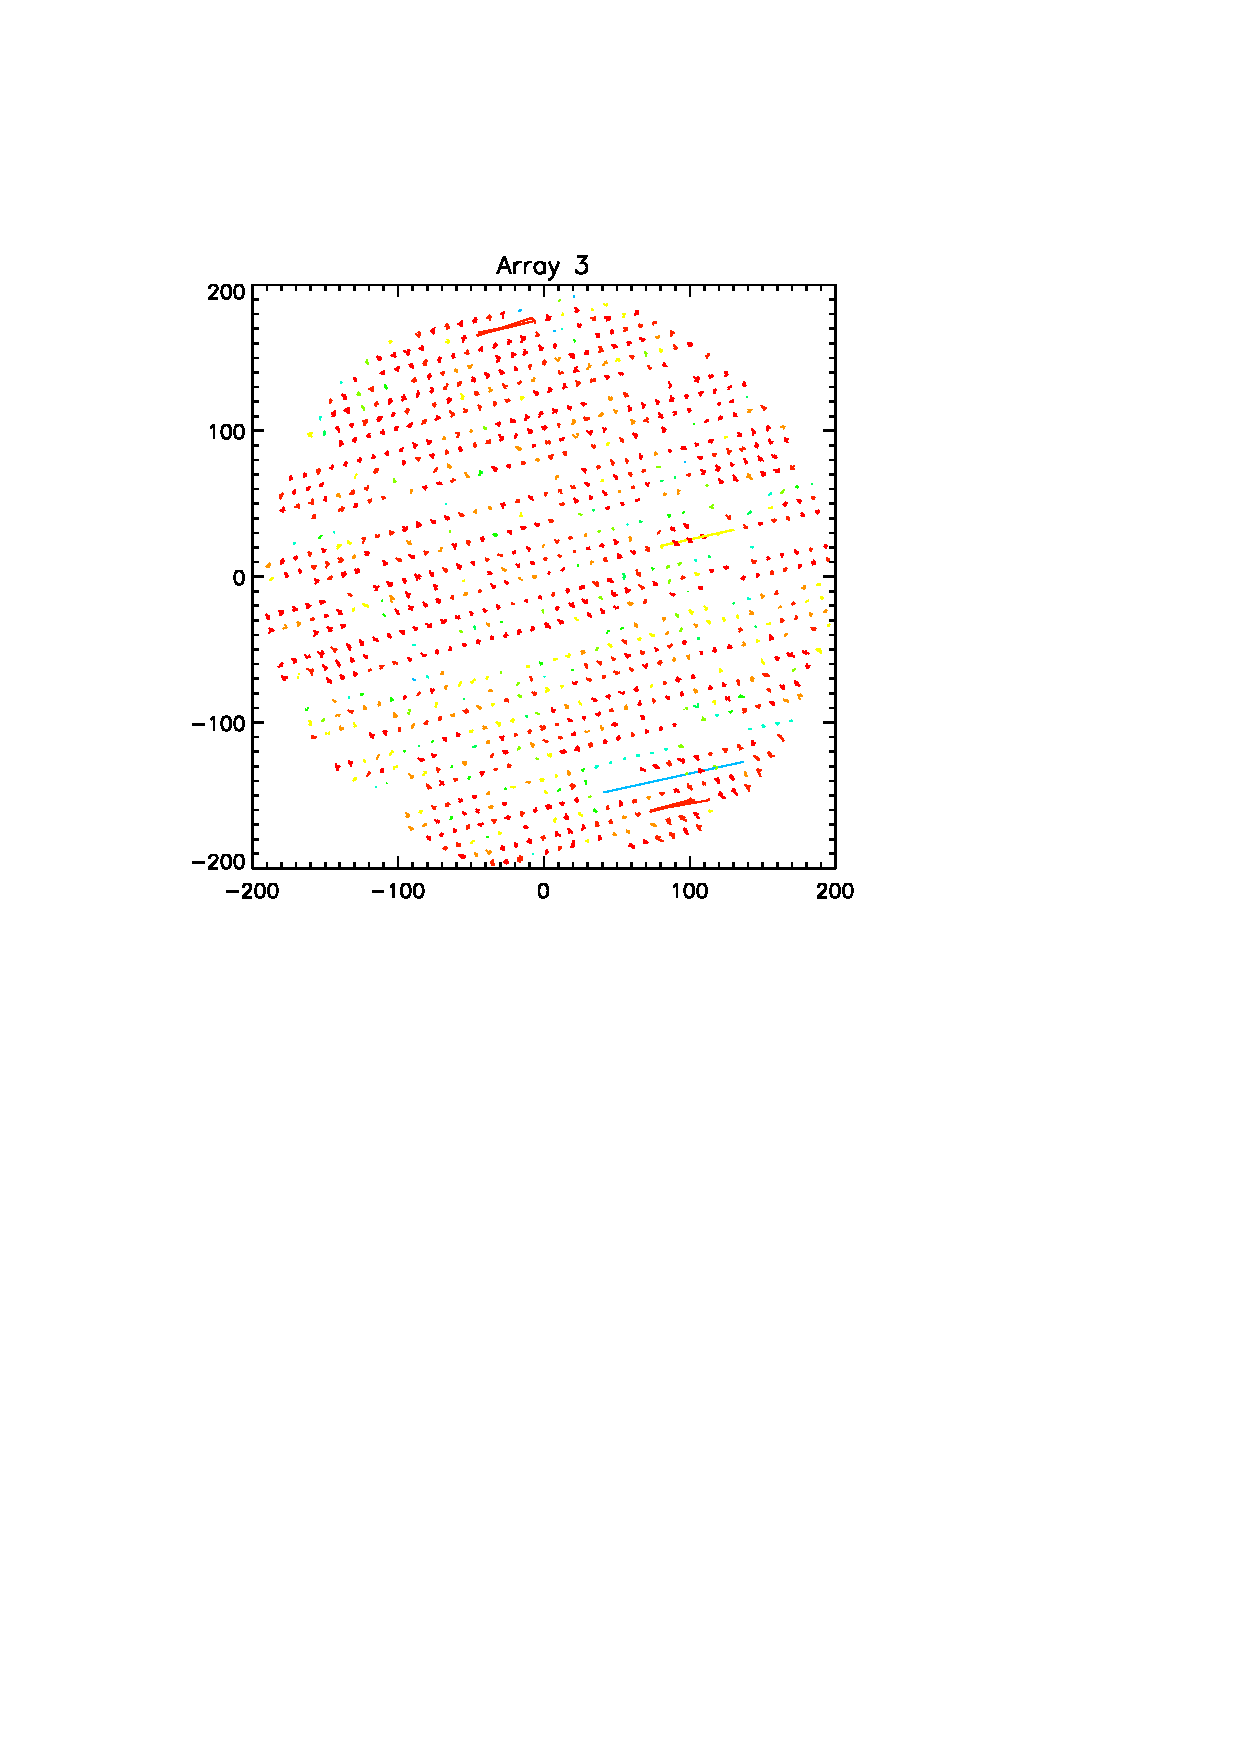
\includegraphics[trim=2cm 14cm 5cm 4cm, clip=true,width=0.55\linewidth]{Figures/A3_positions.pdf}
%% 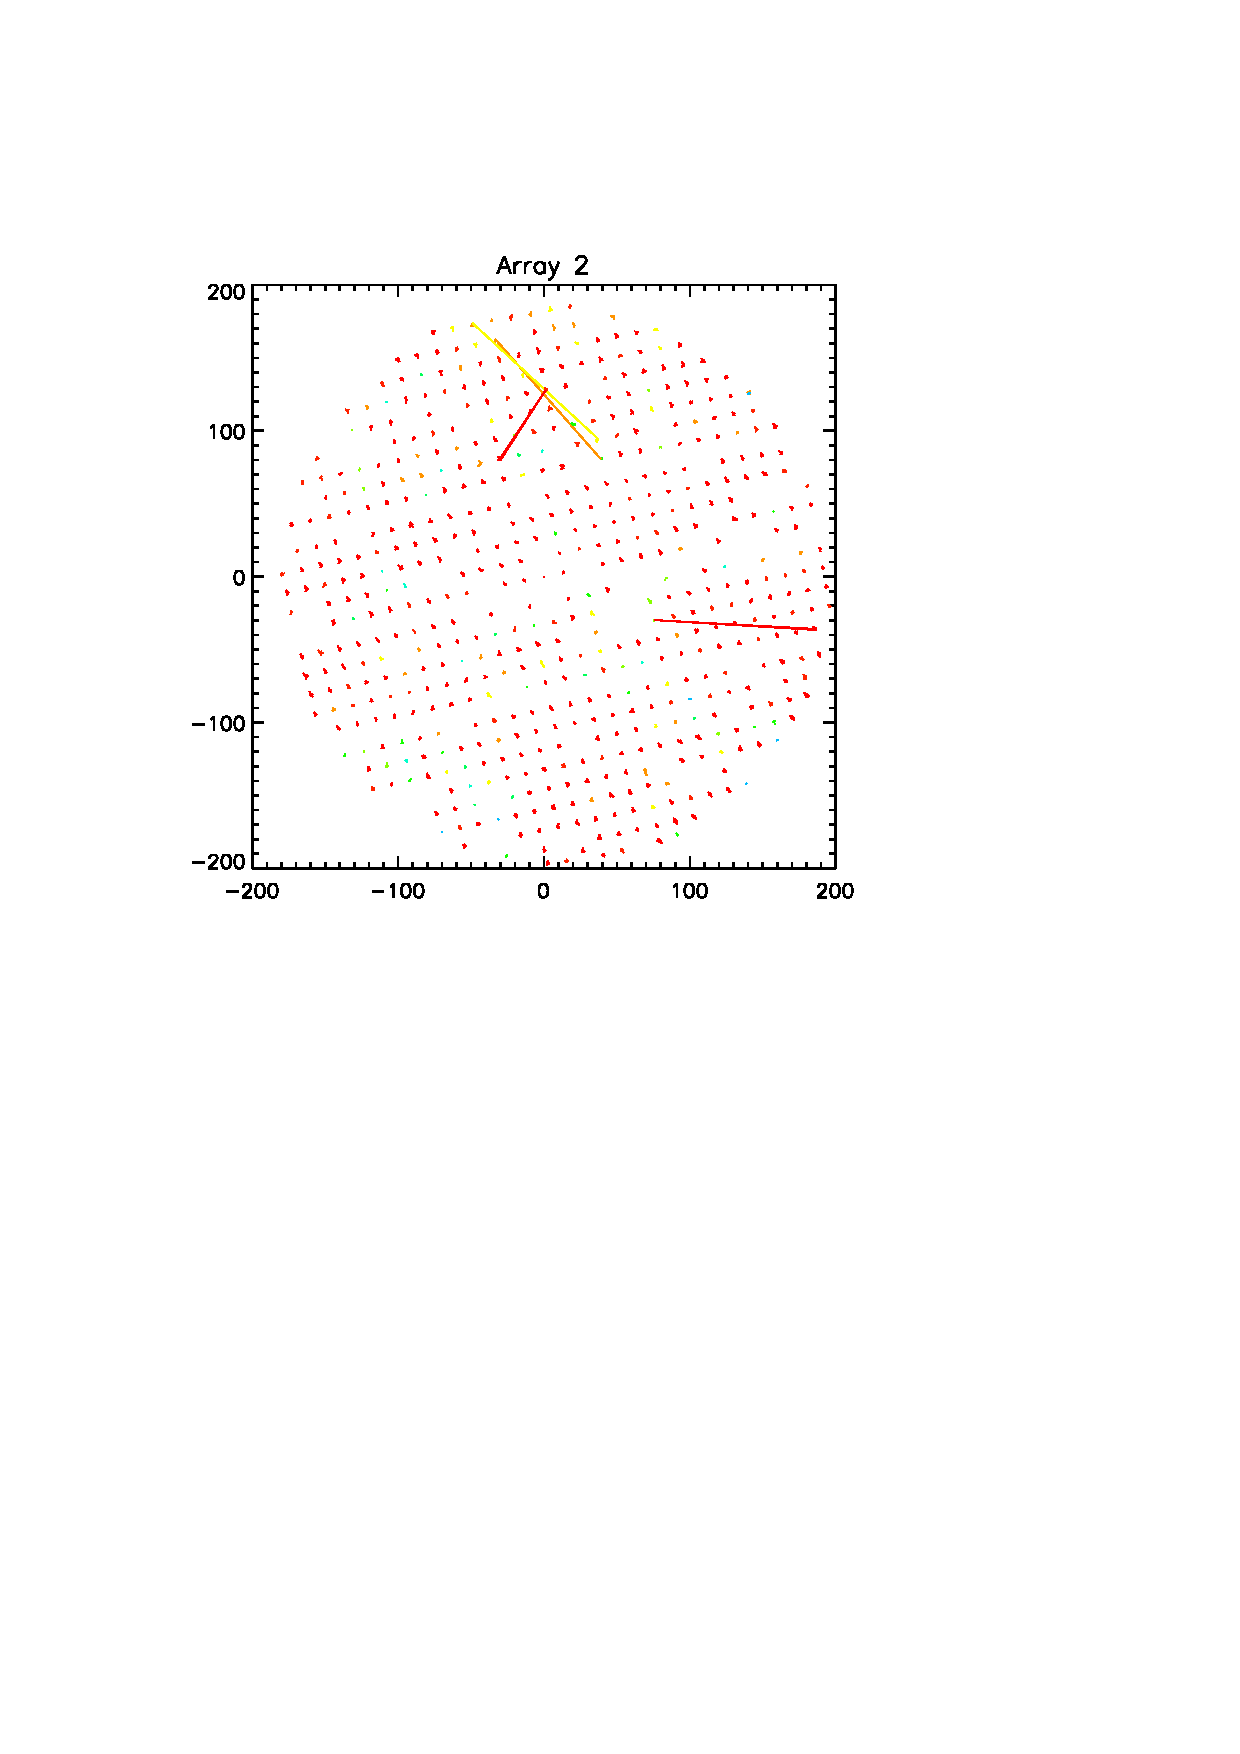
\includegraphics[trim=2cm 14cm 5cm 4cm, clip=true,width=0.55\linewidth]{Figures/A2_positions.pdf}
%% \caption[Stability of KID positions in the field-of-view]{For the valid
%%   detectors, we show the positions of each pixel, as obtained from each beam
%%   map. Some of them are not found at the same position for all the \bms.
%% Units are arcseconds. \todo{{\bf FM : color code : same as on the 1st
%%       maps of validity}}}
%% \label{fig:jumping_kids}
%% \end{center}
%% \end{figure}

%\begin{figure}[htp]
%\begin{center}
%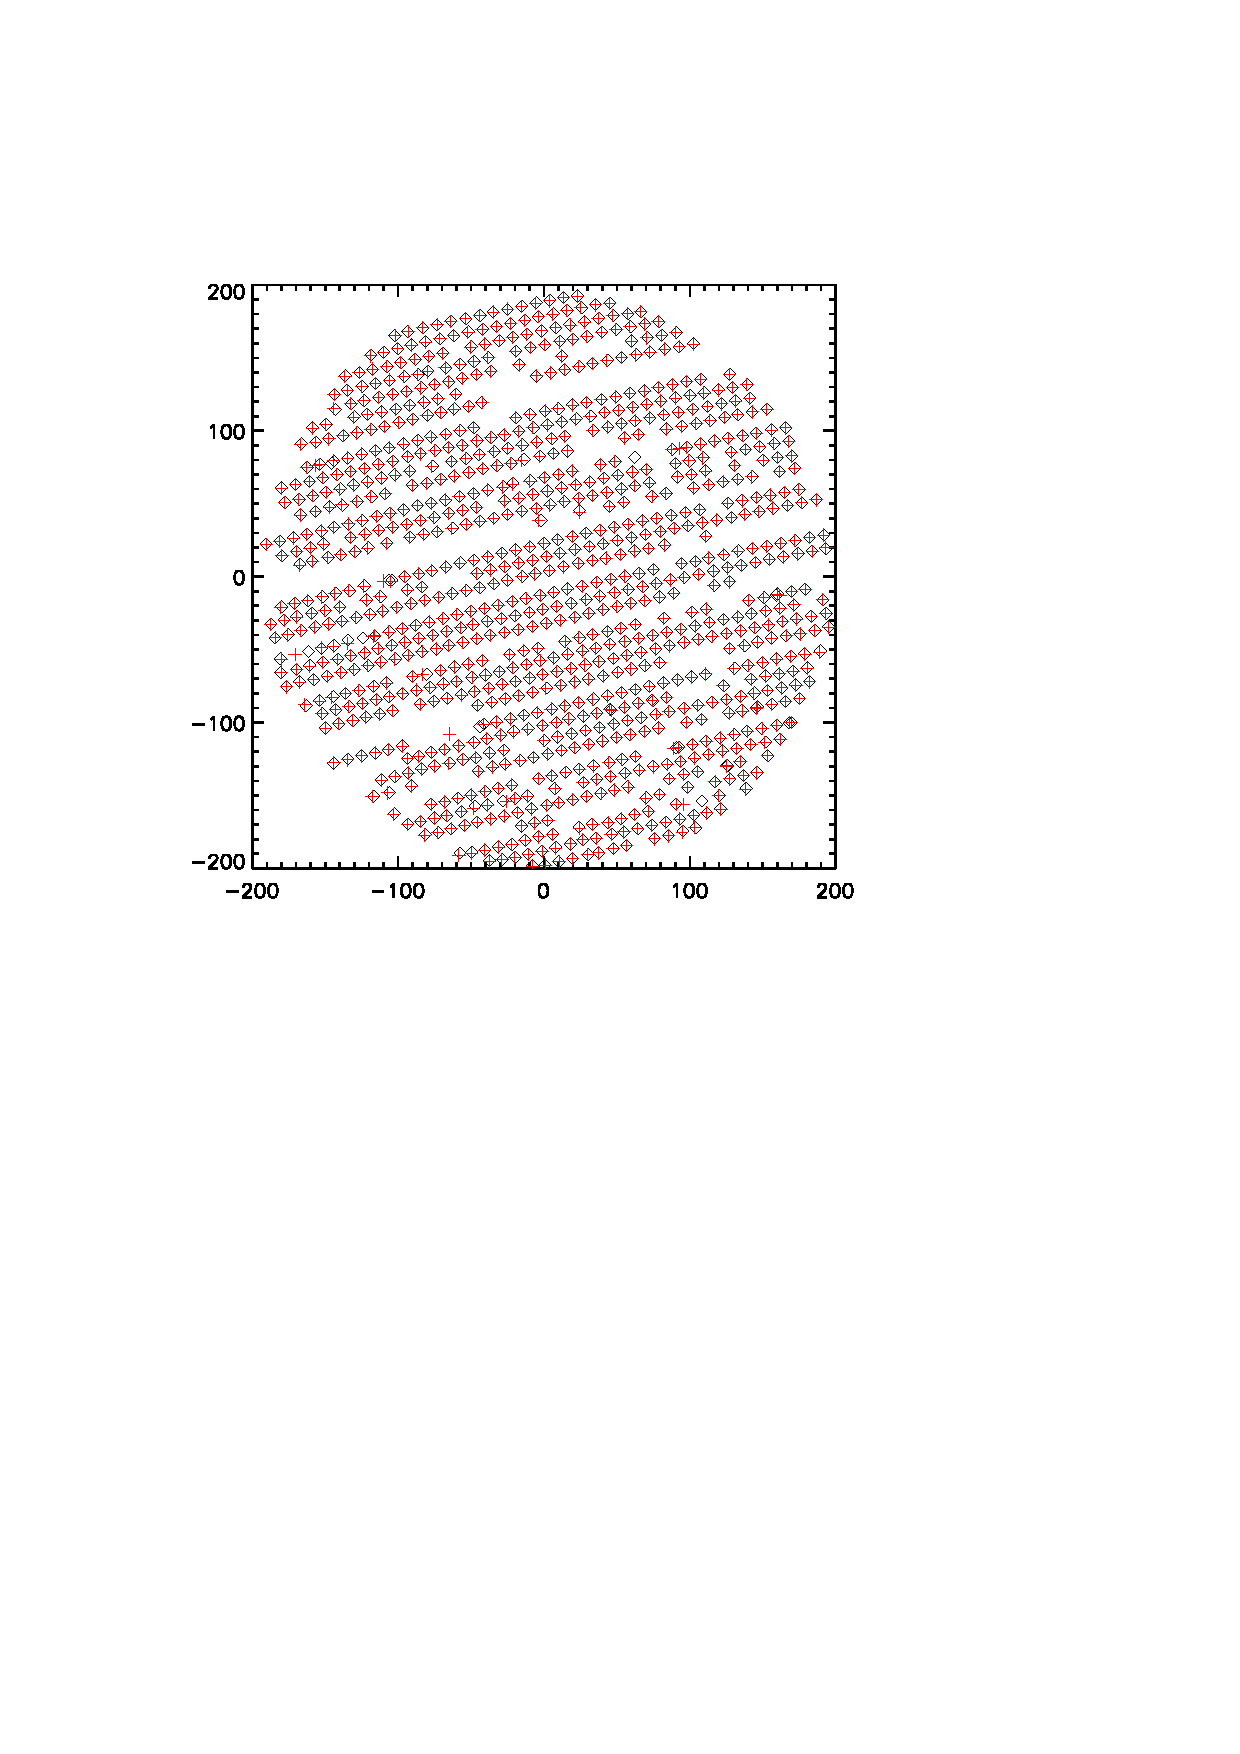
\includegraphics[trim=2cm 14cm 5cm 4cm, clip=true,width=0.55\linewidth]{Figures/A1_test_positions.pdf}
%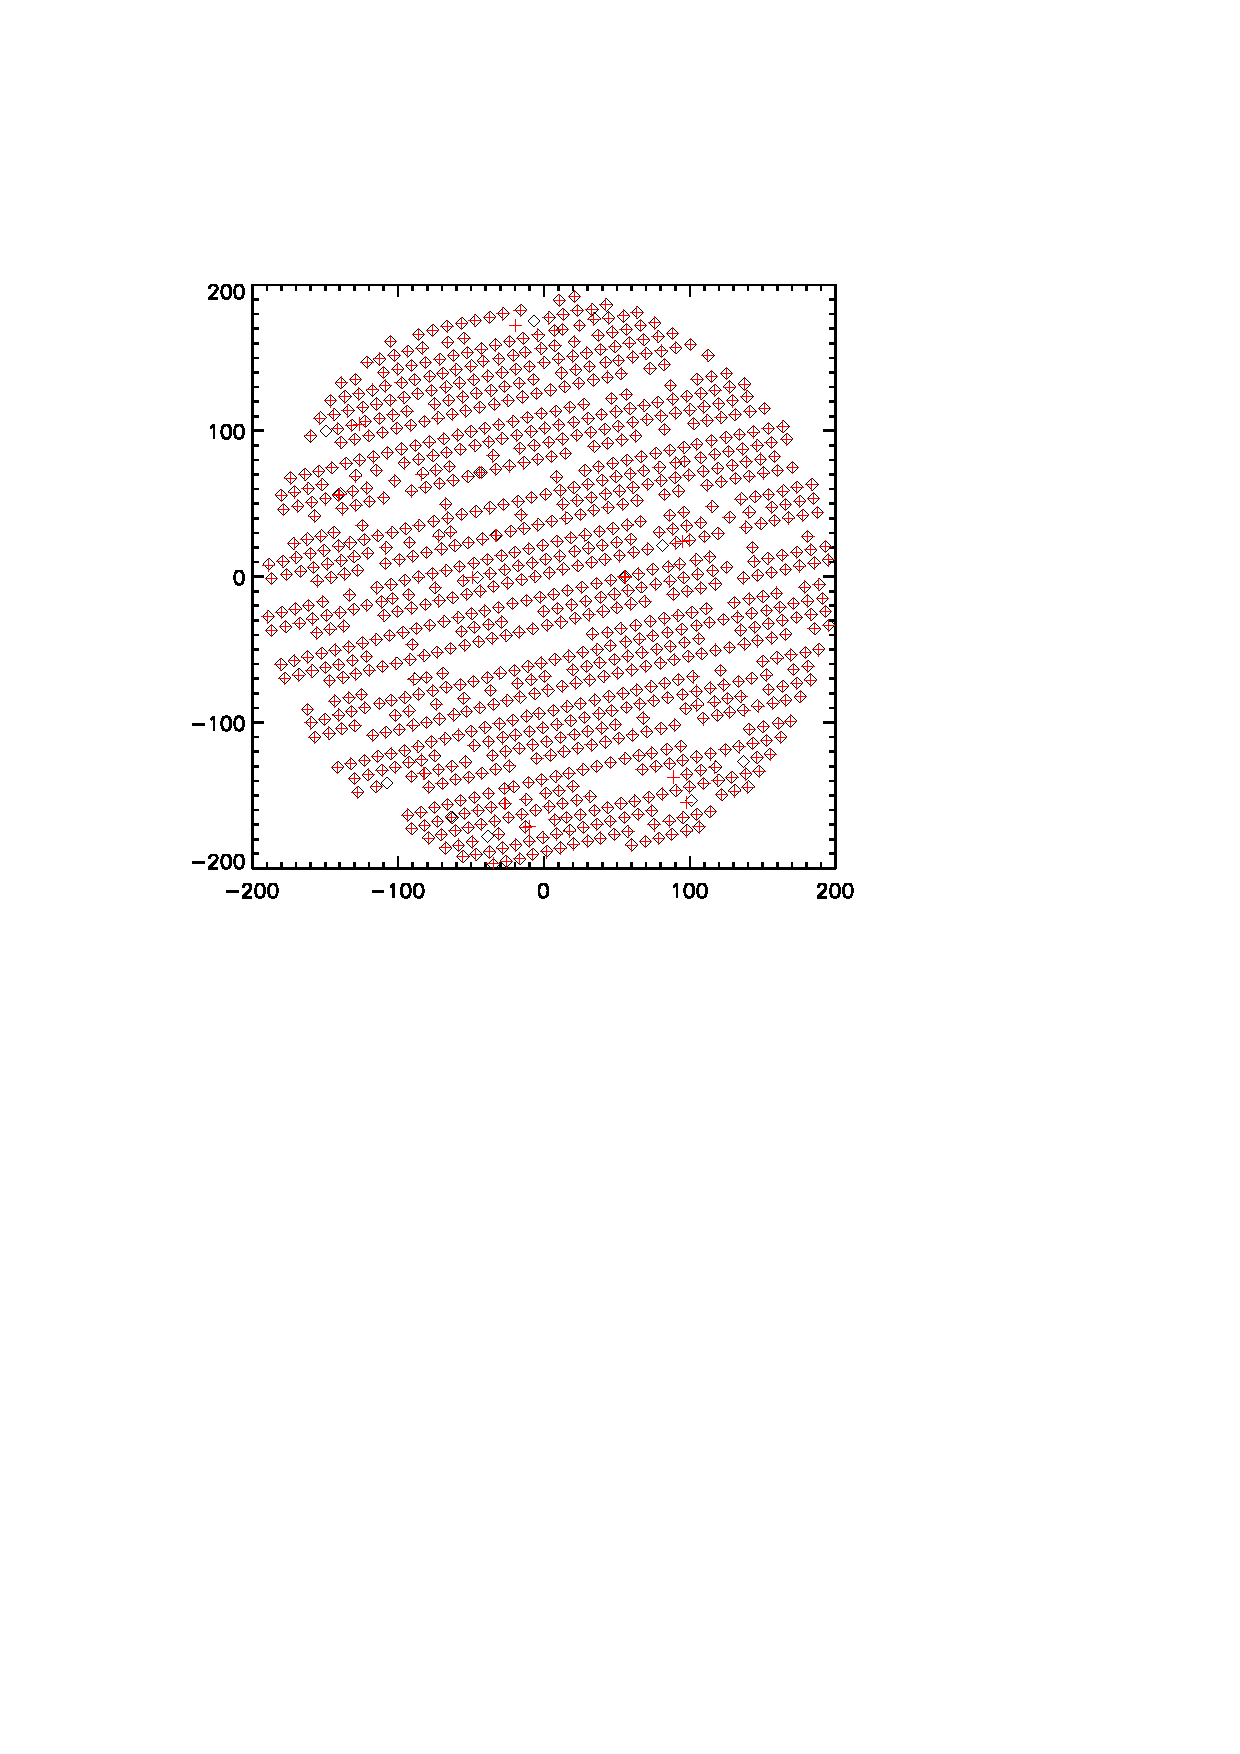
\includegraphics[trim=2cm 14cm 5cm 4cm, clip=true,width=0.55\linewidth]{Figures/A3_test_positions.pdf}
%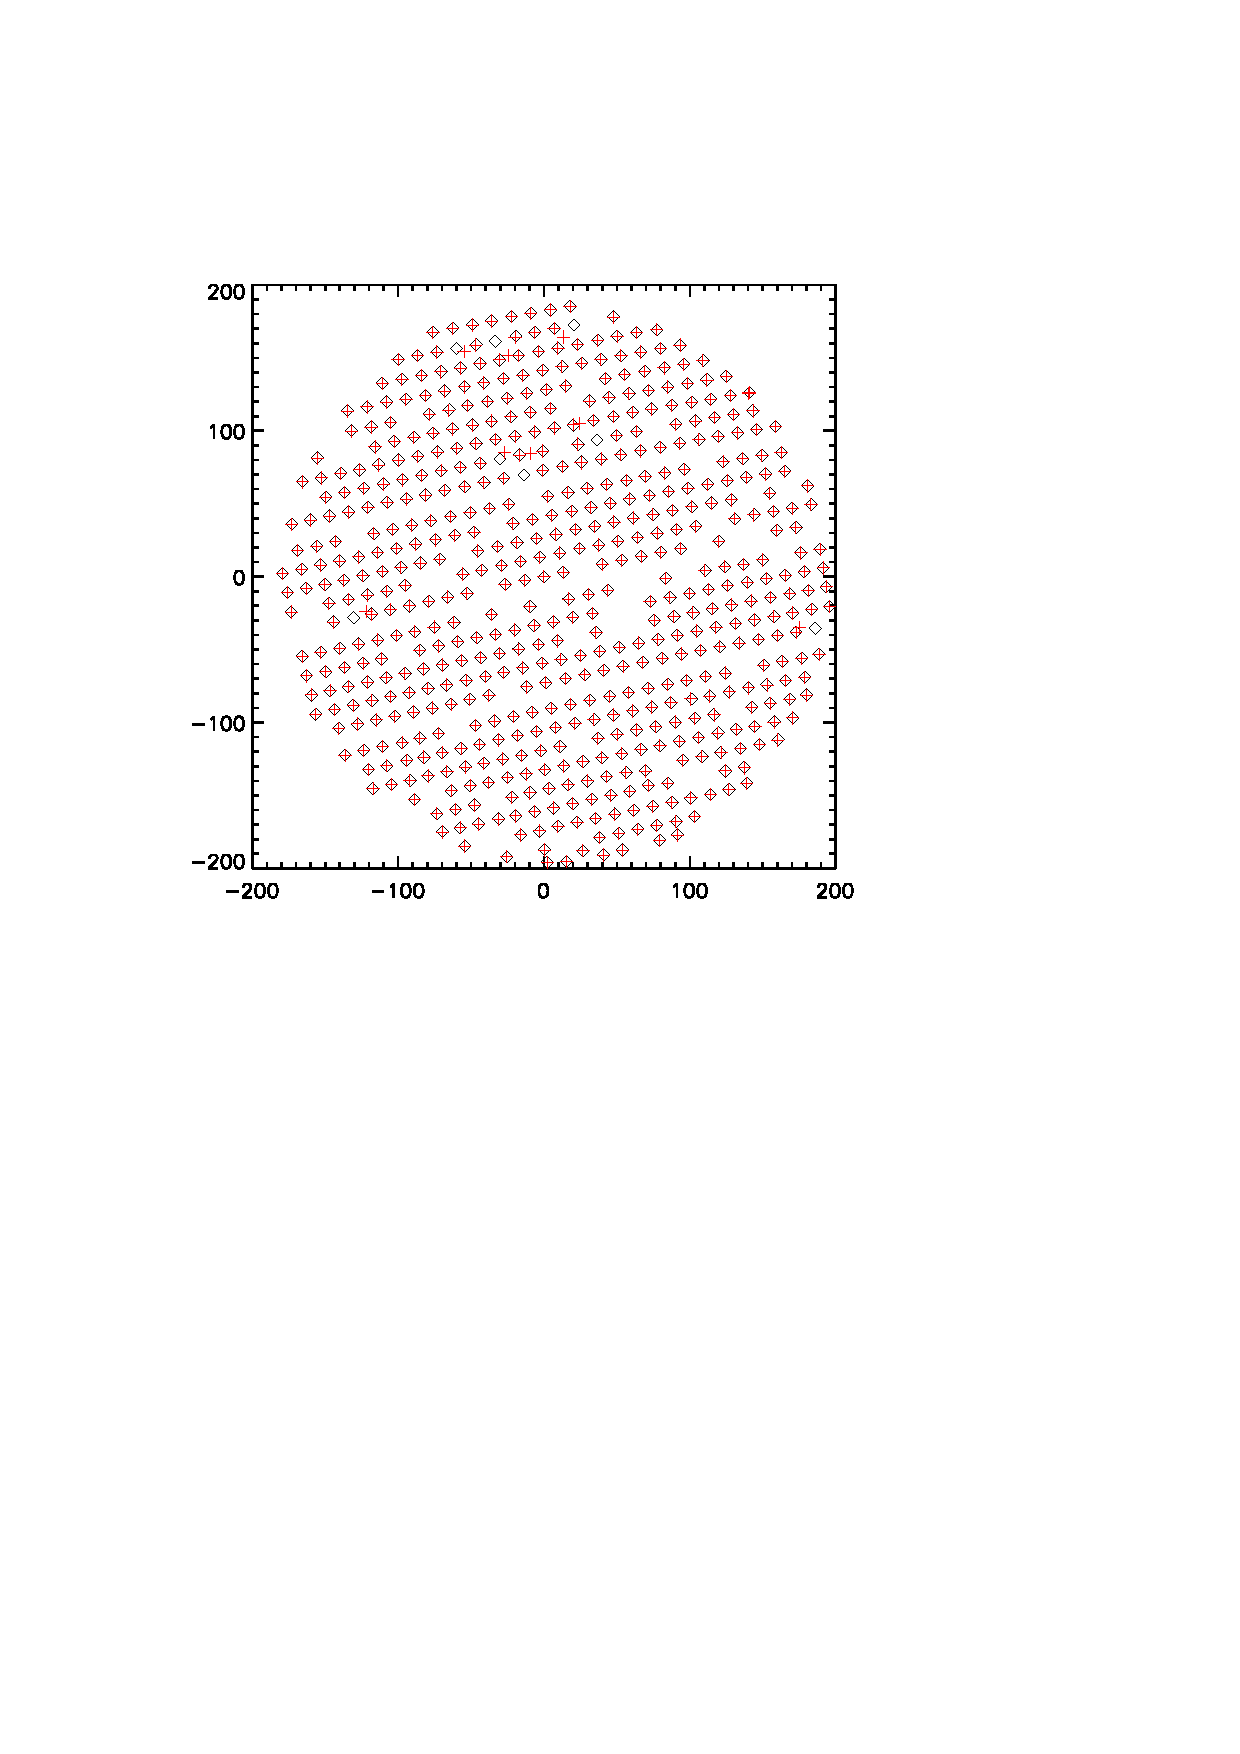
\includegraphics[trim=2cm 14cm 5cm 4cm, clip=true,width=0.55\linewidth]{Figures/A2_test_positions.pdf}
%\caption[Average KID positions]{For the valid detectors,
%  we show the mean (red crosses) and the median (black squares)
%  positions of each pixel, as obtained from each \bm.
%  Units are arcseconds. \todo{FM : color code ? same as on the 1st maps of validity}}
%\label{fig:mean_vs_median}
%\end{center}
%\end{figure}

\begin{table}[!htbp]
  \begin{center}
    \caption[Number of detectors]{Summary of the number of valid detectors per array.}
    \label{tab:number_of_kids}  
    \begin{tabular}{lrrr}
      \hline
      \hline
      \noalign{\smallskip}
      Characteristics & Array 1 & Array 3  & Array 2  \\
      \noalign{\smallskip}
      \hline
      \noalign{\smallskip}
      Design detectors ($N_k$)  & 1140  & 1140   & 616  \\
      Valid detectors           & 952   & 961    & 553  \\ 
      Ratio $\equiv \eta$       & 0.84  & 0.84   & 0.90   \\
      \noalign{\smallskip}
      \hline
    \end{tabular}
  \end{center}    
\end{table}


The valid KIDs, as defined as the KIDs that met the selection
criteria in about one quarter of the FOV geometries, represent the KIDs
usable to produce a scientifically exploitable map of the flux
density using observations for which no sizable {\tt tuning}
issues are experienced. {\lp The valid KID timelines are ingested in
input of the data reduction pipeline. To give an idea of the
dependence of the KID selection on the observing conditions,} we also
evaluate a number of 'very stable' KIDs as the KIDs that met the
selection criteria at least in $70\%$ of the FOV geometries (at least
five times out of seven). We
found 840, 868 and 508 KIDs using this definition for A1, A3 and A2,
respectively. The fraction of very stable KIDs (valid at least five
times) over the designed ones is reported in Table.~\ref{tab:eta_used}.   
\begin{table}[!htbp]
  \centering
  \caption[]{Fraction of \emph{golden} KIDs in percent of the design
  KIDs. The row 'very stable KIDs' gives the fraction of KIDs that have been selected
  in $70\%$ of the analysed {\tt beammap} scans, while the rows 'Used KIDs' gather
  the median fraction of used KIDs in the data reduction processing
  after the conservative KID selection has been performed (see Sect.~\ref{se:dataproc})}
  \label{tab:eta_used}
  \begin{tabular}{llrrrr}
    \hline\hline
    \noalign{\smallskip}
    &  Data set   & A1      &   A3    &     A2 \\
    \noalign{\smallskip}
    \hline
    \noalign{\smallskip}
    Very stable KIDs & {\tt beammaps} & 74  &  76  &  82  \\
    \hline
    \noalign{\smallskip}
    Used KIDs  & N2R9     & 58 &  64  & 71 \\
               & N2R12    & 73 &  69  & 77 \\
               & N2R14    & 69 &  68  & 79 \\
               & Combined & 70 &  69  & 78 \\
    \hline
  \end{tabular}
\end{table}

Practically, for the production of flux density maps, we perform
further selection of the valid KIDs using a conservative noise level
thresholding of the KIDs at the \emph{low level processing}, as discussed in
Sect.~\ref{se:dataproc}. The number of used KIDs for producing
science-purpose maps using the data reduction pipeline, as described
in Sect.~\ref{se:dataproc}, is thus significantly lower than the number of
valid KIDs. We evaluate the median number of used KIDs using all scans
for each of the observation campaigns. The median fractions of used
KIDs with respect to the design ones for each campaigns and for the
combinations of all scans are given in Table.~\ref{tab:eta_used}. We
find median fractions of used KIDs of about $70\%$ for the
$1\, \rm{mm}$ arrays and of about $80\%$ for the $2\, \rm{mm}$ array,
with a notable exception at the N2R9 technical campaign, for which
these fraction are lower due to severe temperature-induced instable
observing conditions (see Sect.~\ref{se:beam_variation}). Moreover the
median fractions of used KIDs are close to the fractions of
very stable KIDs from the FOV geometries. We stress that these numbers
depend on the choices made in the data reduction pipeline for data
sample cuts, and are thus subject to improvement. By contrast, the
fractions of valid KIDs $\eta$ constitute a conservative estimates of the
stable KIDs usable for science exploitation over all the fonctionning
KIDs. These are thus the relevant estimates for the instrument
performance assessment.  
 


%----------------------------------------------------------------------------------------
%	6./ Beam Pattern
%----------------------------------------------------------------------------------------
\section{Beam Pattern}
\label{se:beam}
%----------------------------------------------------------------------------------------
%	6./ Beam Pattern
%----------------------------------------------------------------------------------------
%\section{Beam Pattern}
%\label{se:beam}

%The NIKA2 beam pattern mainly depends on the IRAM \trentemetre\ telescope and
%NIKA2 full (external and internal) optical system characteristics,
%whereas the detectors themselves have an impact at sub-dominant
%level (through \emph{e.g.} the KID size, time constants or correlated noise).
%It is important to specify that the detectors impact on the size of the
%beam pattern, when you include the size of the pixel, and on the
%measure of the beam pattern with their time constants and noise.
{\lp The NIKA2 beam pattern is given by the KIDs illuminating the internal
and external optics, out to the IRAM \trentemetre\ telescope primary mirror.}
The full beam pattern is characterized using \bm\ observations. First,
we produce deep integration maps of bright sources to provide a
qualitative description of the complex beam structure in
Sect.~\ref{se:fullbeam}. Then we model the beam using three
complementary methods to estimate the main beam angular resolution
(Sect.~\ref{se:mainbeam}) and the beam efficiency
(Sect.~\ref{se:beam_efficiency}).

\subsection{Full beam pattern}
\label{se:fullbeam}

We study the two-dimensional pattern of the beam using \bms. We
primarily use a map obtained from a combination of \bm\ observations
of strong point sources collected during
N2R8 and N2R9 technical campaigns. Namely, we use \bm\ scans
of Uranus%(scan id '20170125s223' and '20170125s243')
,  Neptune %('20170224s177')
and the bright quasar 3C84. %('20170226s415').
Furthermore, we checked the stability of our results on single scan
maps, combinations of scans for a single source, and combinations of
shallower scans but spanning a large range of scanning direction. 
{\lp Figure~\ref{fig:features} shows the two-dimensional beam pattern
as measured with NIKA2 using the former \bm\ combination, for each of
the arrays and for the $1\,\rm{mm}$ array combination.}
{\lp The beam pattern is shown over a large dynamic range down
to about $-40\,\rm{dB}$ and out to radii of about 5’.
The telescope beam pattern further extends well beyond this radius, as for
example shown by lunar edge observations
%with heterodyne front-ends installed
at the IRAM \trentemetre\ telescope~\citep{Greve1998,
Kramer2013}. However,
this extended pattern is at present difficult to detect using the data
reduction pipeline discussed in Sect.~\ref{se:dataproc}, as
the extended error beams are both filtered and mixed with 
atmospheric and electronics large-scale correlated noise
residuals. The large angular scale contributions to the full beam are
further discussed in Sect.~\ref{se:beam_efficiency}.} 
%are difficult to distinguish from common mode variations of the atmosphere or electronics.}


%The data processing includes a mitigation of the correlated noise, which
%mainly originates from the atmosphere.  We primarly use a subtraction
%of a common mode estimated from the most correlated detectors (the
%so-called 'cm one block' method). However, other methods are tested
%for assessing the immunity of our results to noise residuals.

%\begin{figure}[!thbp]
%\begin{center}
%  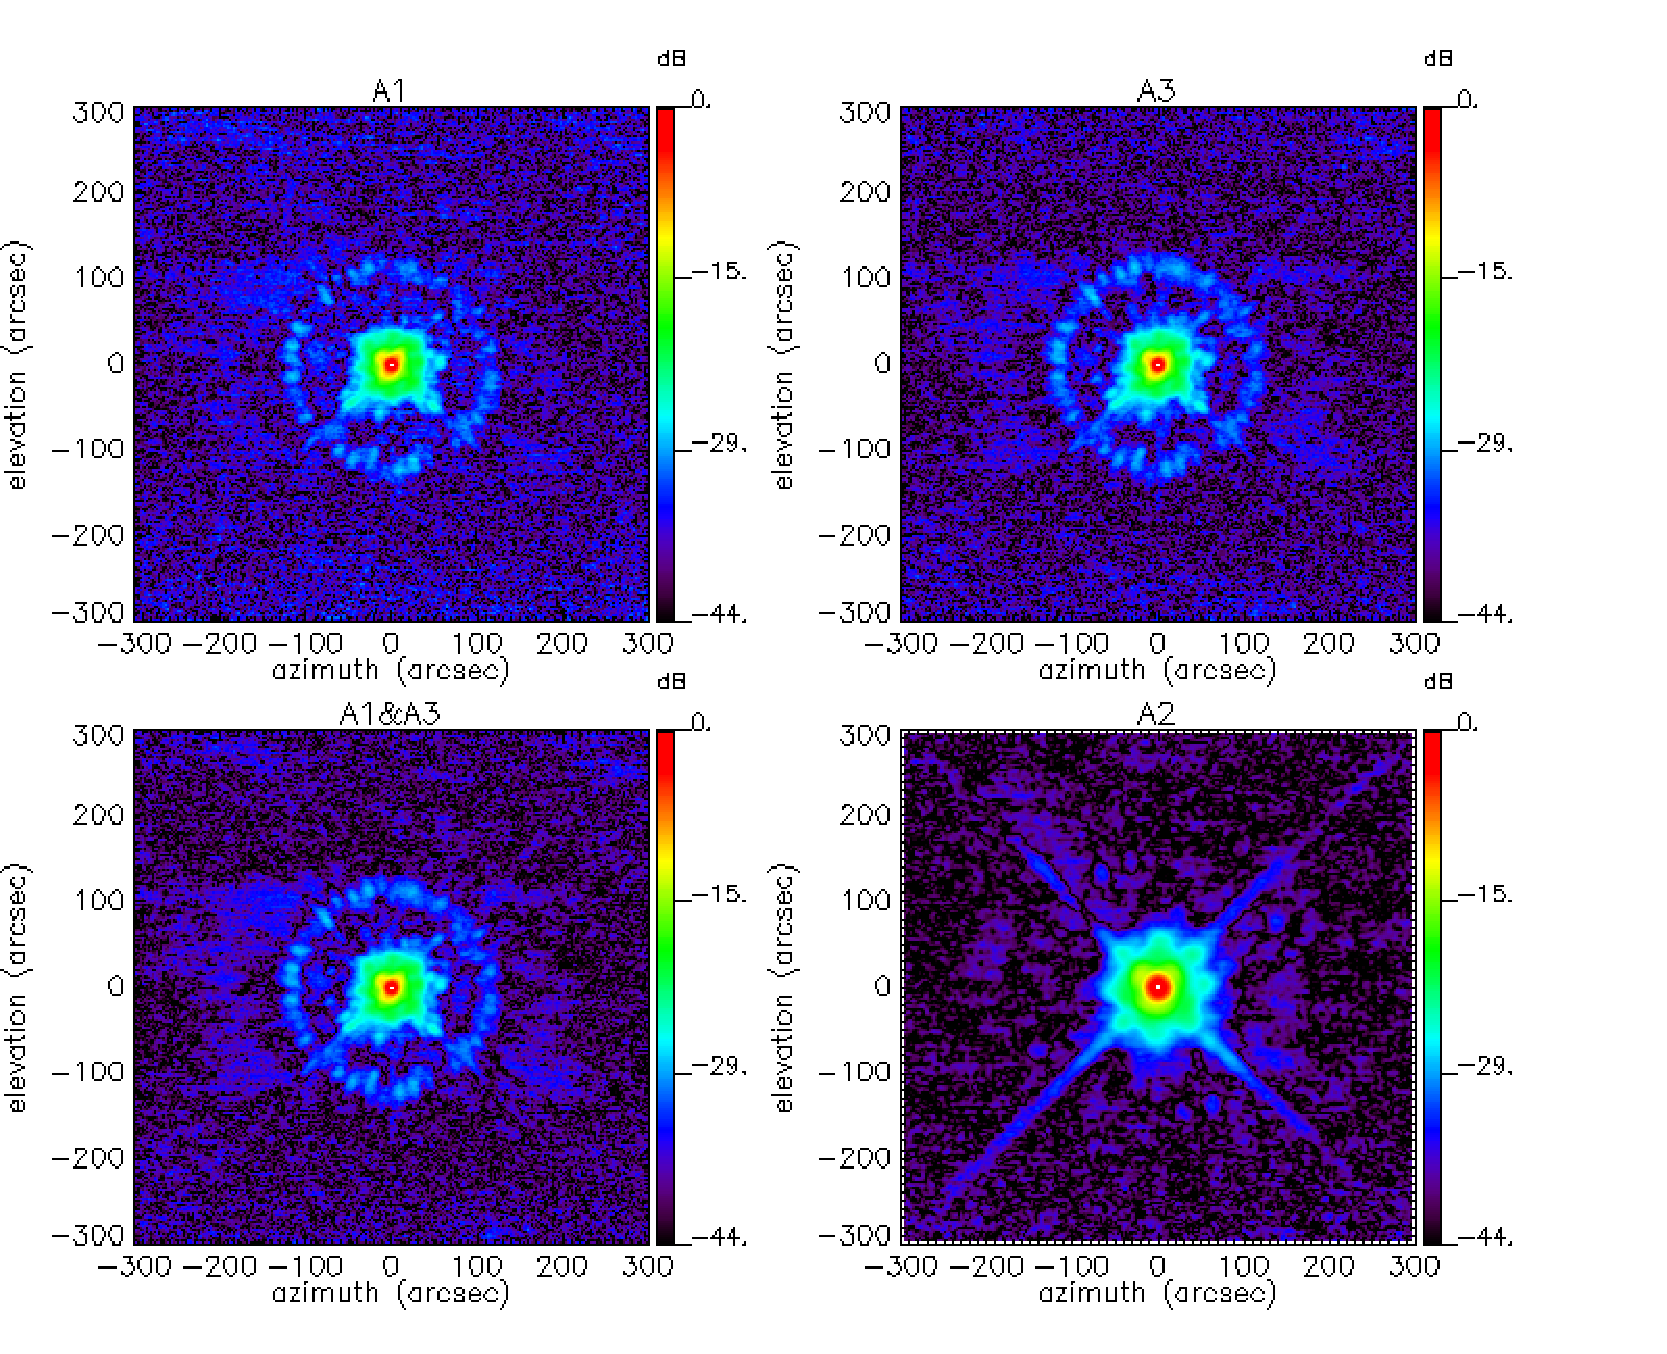
\includegraphics[trim=0cm 0cm 2.5cm 0cm, clip=true, width=\linewidth]{Figures/Lobe_map_Combo_v2_dB.pdf}
% \caption[Beam pattern.]{From upper left to lower right, beam maps of array 1 (labeled 'A1'), array 3 ('A3'), the combination of the $1\,\rm{mm}$ arrays ('A1$\&$3') and the  $2\,\rm{mm}$ array ('A2') are shown in decibel. These maps, which consist of normalized combination of four long OTF scans of bright point sources, are in horizontal coordinates and cover a sky area which extends over 10 arcmin.}
%\label{fig:beam}
%\end{center}
%\end{figure}

\begin{figure}[!thbp]
\begin{center}
  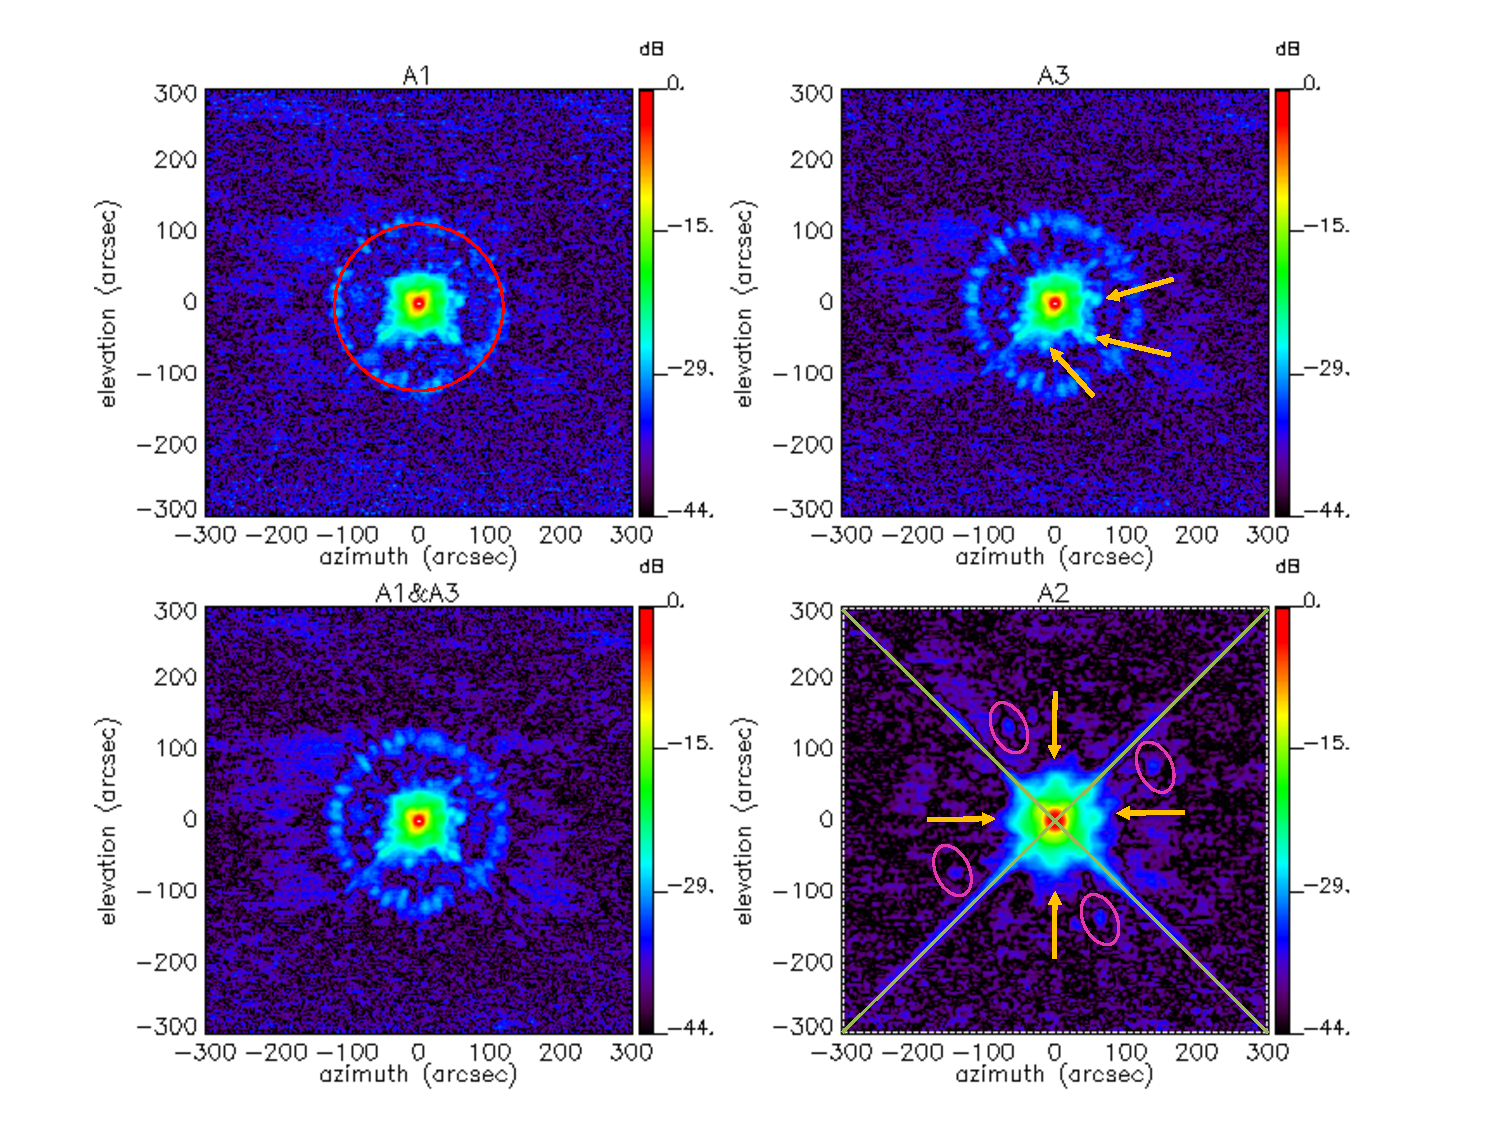
\includegraphics[trim=0.5cm 0.5cm 1cm 0cm, clip=true, width=\linewidth]{Figures/Beams_features.pdf}
\caption[Noticeable features of NIKA2 beam pattern.]{From upper left
  to lower right, beam maps of A1, A3,
  the combination of the $1\,\rm{mm}$ arrays (A1$\&$3) and the
  $2\,\rm{mm}$ array (A2) are shown in decibel. These maps, which
  consist of the normalized combination of four {\tt beammap} scans of
  bright point-like sources, are in horizontal coordinates and cover a
  sky area which extends over $10'$. %Same maps as in Fig.~\ref{fig:beam}
  %with some noticeable features.
  The solid lines and arrows highlight some noticeable features.
  Red circle in the A1 map (upper left panel): diffraction ring seen in 1-mm maps
  (the spokes are presumably caused by radial and azimuthal panel
  buckling \citep{Greve2010}; Orthogonal green lines in the A2 map
  (lower right panel): diffraction
  pattern caused by quadrupod secondary support structure (prominently
  seen in A2 map); Yellow arrows in the A3 map (upper right panel):
  pattern of 3 spikes seen in $1\,\rm{mm}$ maps of unknown origin; Yellow
  arrows in A2 map (lower right panel): four symmetrical spikes of the
  first sidelobes; Pink ellipses: four spikes seen in A2 maps.}
\label{fig:features}
\end{center}
\end{figure}

The NIKA2 beam maps reveal some noticeable features, which are
shown in Fig.~\ref{fig:features}. Ranging from strong and/or extended to
weak and/or spiky, they include:
\begin{enumerate}
\item the main beam and the underlying first error
  beam, which is due to large-scale deformations of the primary
  mirror, and the first side lobes, {\lp which correspond to various diffraction
  patterns. In particular, the 60'' and 85'' diameter (squarish) side
  lobes at $1$ and $2\,\rm{mm}$, respectively, at a level lower than
  $-20\,\rm{dB}$, are due to the convolution of the primary mirror and
  quadrupod diffraction pattern with the pixel (KID) transfer function;}
  %The latter include 
  %the 20" diameter first side lobe and the 60" diameter (squarish)
  %side lobe, which is due to the convolution of the primary mirror and
  %quadrupod diffraction pattern with the pixel (KID) transfer function;
  %The four symmetrical spokes of the error beam as shown by
  %yellow arrows in the A2 panel, are expected from ZEMAX
  %simulations;
   %The 20”/60” “lobes” refer to 1mm or 2mm ? Here, we mixing the terms
  %“error beams” and “side lobes”. Aren’t the 20” diameter “1st side
  %lobe” and the “1st error beam” the same ?  To my understanding, side
  %lobes show up in the maps as rings, e.g. diffraction patterns. Error
  %beams, on the other hand, show-up as broad Gaussians entered on the
  %main beam. The section on the radial averages should take up the
  %discussion of 20” and 60” diameter error beams, and actually show
  %them in the figures.
\item at a much lower level of about $-30\,\rm{dB}$, a diffraction ring shows    
up, which is presumably caused by panel buckling of the primary 
  mirror~\citep{Greve2010}, as shown with a red circle in the A1 panel;
\item also at a level of about $-30\,\rm{dB}$, the side lobes shown with green
  diagonal lines in the A2 panel are due to diffraction on the
  quadrupod holding the secondary mirror of the telescope, as expected
  from ZEMAX simulations;  
\item spikes of not fully understood origin marked by yellow
  arrows. The ones that are along the vertical and
  horizontal axes are reproduced by ZEMAX simulations but at a 
  shallower level, whereas the ones shown in the A3 panel in the
  diagonal directions may be due to the small cylindrical
  instrumentation box on the side of the M2 cabin. The origin of the
  asymmetry on the 1~mm arrays is unknown but most probably due to
  internal optics aberrations;
\item shallow spikes of unknown origin at a level less than $-30\,\rm{dB}$, which are circled by pink
  ellipses. The multiple images on the combined deep beam map indicate
  a rotation of these spikes with the observing elevation, which in
  turn point to diffraction related issue or a ghost image that are
  formed inside the cryostat. These shallow features are expected to
  have no sizable impact on NIKA2 science results.
\end{enumerate}

We further quantify the respective level of the axi-symmetrical
features of the beam pattern by evaluating the beam radial profile
$B(r)$, which is the normalised radial brightness profile,
where $r$ is the radius from the beam center.
%is the azimuthal average of the beam map around the
%main beam center.
Although the profile cannot represent the sub-dominant non-axisymmetrical
features, which are seen in Fig.~\ref{fig:features} (quadrupod
diffraction pattern, spikes), it provides a useful
representation of the internal and central parts of the beam (about up to
$100''$). We determine a beam profile from a beam map in centering to
the fitted value of the main beam center and in forming the
weighted average of the map pixels in annular rings.

We checked the stability of the beam against various
observing conditions (source intensity, weather condition, focus
optimisation) by comparing the beam profiles of a series of 18 \bm\
observations.
This set of \bms, which is referred to as {\tt BM18}, has been
selected from all the available \bm\ scans at optimal focus using the
baseline scan selection criteria, as given in
Sect.~\ref{se:data_selection}.
%The 18 beam profiles and their difference w.r.t. the median beam
%profile are shown in Fig.~\ref{fig:beam_prof}.
The measured beam profiles using the {\tt BM18} data set are shown in
Fig.~\ref{fig:beam_prof}. Calculating the {\lp rms of the relative}
difference of the beam profiles to the median beam profile, we find a
dispersion below $5\%$ at $1\,\rm{mm}$ and below $2\%$ at
$2\,\rm{mm}$.

{\lp To measure the relative level of the axi-symmetrical beam pattern
features, we further model the beam profiles using an empirical function,
which accounts for the main beam and for a significant fraction of the
error beams and side lobes. This function consists in a three-Gaussian
function $B(r)$ defined as:
\begin{equation}
  B(r) = \sum_{i=1}^{3} \mathcal{A}_i G_i(r) + \mathcal{B}_0,
  \label{eq:3gauss}
\end{equation}
where $\mathcal{A}_i$ is the amplitude of the Gaussian $i$ for
$i \in {1, 2, 3}$ and $\mathcal{B}_0$ a pedestal level accounting for
the residual background level in the map. The measured beam profiles
are fitted using Eq.~\ref{eq:3gauss} and the median best-fit
parameters are given in Table~\ref{tab:mean_3gauss_fit}. These values
are given to gain insight of beam profile, but are not further used
for the calibration.
%
% AVERAGE 3-GAUSSIAN FIT
\begin{table}[!th]
   \caption{{\lp Median best-fitting values of the parameters of the
  3-Gaussian beam profile, as defined in Eq.~\ref{eq:3gauss}, using
  the {\tt BM18} data set. $\bar{\mathcal{A}_i}$, for
  $i \in {1, 2, 3}$ are the Gaussian amplitudes $\mathcal{A}_i$ relative to the sum
  of $\mathcal{A}_i$, and given in decibel. The FWHM for each of the Gaussian are given in arcseconds. The errors are evaluated as the standard deviation of the best-fitting parameter values of the 18 \bm\ scans of {\tt BM18}.}}
  \label{tab:mean_3gauss_fit}
  \begin{center}
    \begin{tabular}{rll}
      \hline\hline
      \noalign{\smallskip}
%      & \multicolumn{6}{c}{3-Gaussian profile parameters}  \\\cline{1-7}
%      Arrays       & Amp 1 & Amp 2 & Amp 3 & FWHM 1 & FWHM 2 & FWHM      3 \\
       parameters  &  $1\,\rm{mm}$  & $2\,\rm{mm}$ \\
       \noalign{\smallskip} 
      \hline
      \noalign{\smallskip} 
      $\bar{\mathcal{A}_1}$ [dB] &   $-0.33 \pm 0.09$   &  $-0.24 \pm 0.03$ \\
      $\bar{\mathcal{A}_2}$ [dB] &   $-11.4 \pm 1$     &  $-12.8 \pm 0.5$   \\
      $\bar{\mathcal{A}_3}$ [dB] &   $-26 \pm 7$       &  $-27 \pm 3$    \\
      FWHM$_1$  ['']             &   $10.8 \pm 0.2$    &  $17.4 \pm 0.6 $ \\
      FWHM$_2$  ['']             &   $30 \pm 2$        &  $42 \pm 3 $ \\
      FWHM$_3$  ['']             &   $81 \pm 10$       &  $99 \pm 7 $ \\     
%      A1        &  $0.89 \pm 0.01$   &  $0.08 \pm 0.02$  & $5 \times 10^{-3} \pm 2 \times 10^{-3}$  &  $11.0 \pm 0.2 $ & $29 \pm 2 $  & $65 \pm 15 $ \\  
%      A3        &  $0.90 \pm 0.01$   &  $0.07 \pm 0.01$  & $4 \times 10^{-3} \pm 2 \times 10^{-3}$  &  $11.0 \pm 0.2 $ & $30 \pm 3 $  & $72 \pm 23 $ \\  
%      1mm       &  $0.90 \pm 0.01$   &  $0.07 \pm 0.01$  & $4 \times 10^{-3} \pm 2 \times 10^{-3}$  &  $11.0 \pm 0.2 $ & $29 \pm 2 $  & $70 \pm 15 $ \\  
%      2mm       &  $0.96 \pm 0.01$   &  $0.3 \pm 0.3$    & $1 \times 10^{-3} \pm 0.3$ &  $17.5 \pm 0.1 $ & $63 \pm 10 $ & $65 \pm 12 $ \\
       \noalign{\smallskip}   
      \hline
    \end{tabular}    
  \end{center}
\end{table}
%

For illustration, we show the median best-fit
three-Gaussian profiles at $1$ and $2\,\rm{mm}$ with pink lines, and
the main beam (first Gaussian) profiles with black lines in
Fig.~\ref{fig:beam_prof}. 
}


%%%%%%%%%%%%%%%%%%%%%%%%%%%%%%%%%%%%%%%%%%%%%%%%%%%%%%%%%%%%%%%%%
% Stability of the beam pattern
\begin{figure}[!thbp]
  \centering
%   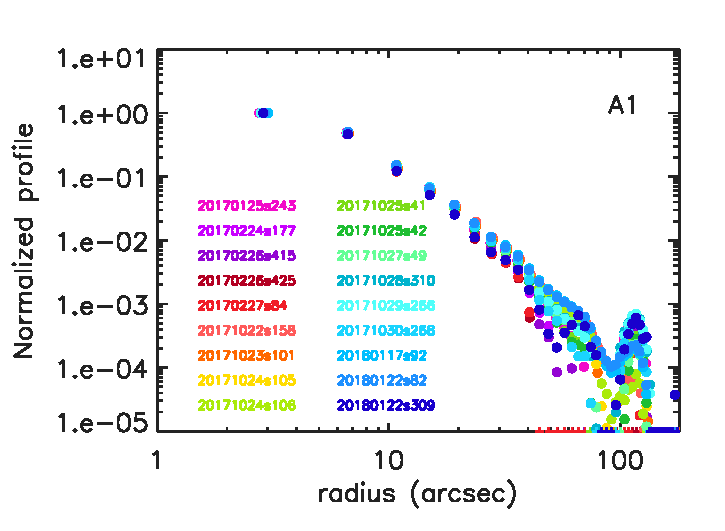
\includegraphics[clip, width=0.42\textwidth]{Figures/Beams/plot_profiles_a1.pdf}
%   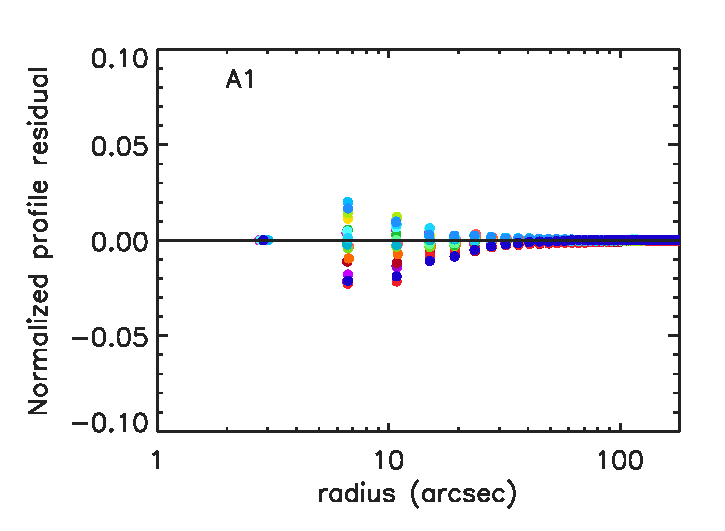
\includegraphics[clip, width=0.42\textwidth]{Figures/Beams/plot_profile_diff_wrt_median_a1.pdf}
%   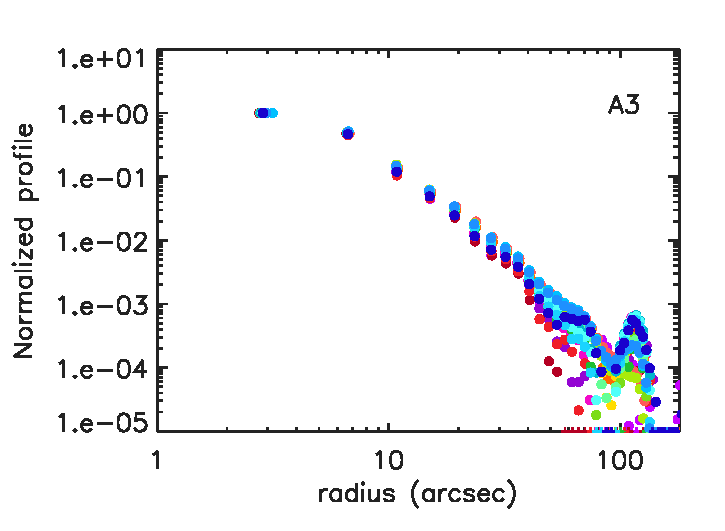
\includegraphics[clip, width=0.42\textwidth]{Figures/Beams/plot_profiles_a3.pdf}
%   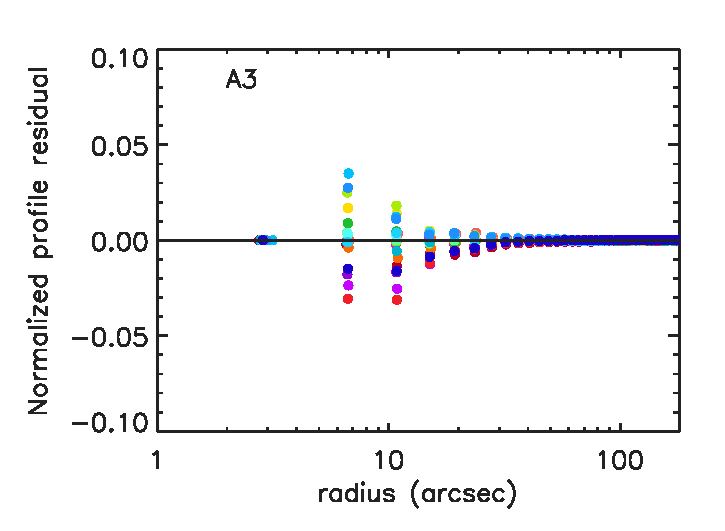
\includegraphics[clip, width=0.42\textwidth]{Figures/Beams/plot_profile_diff_wrt_median_a3.pdf}
   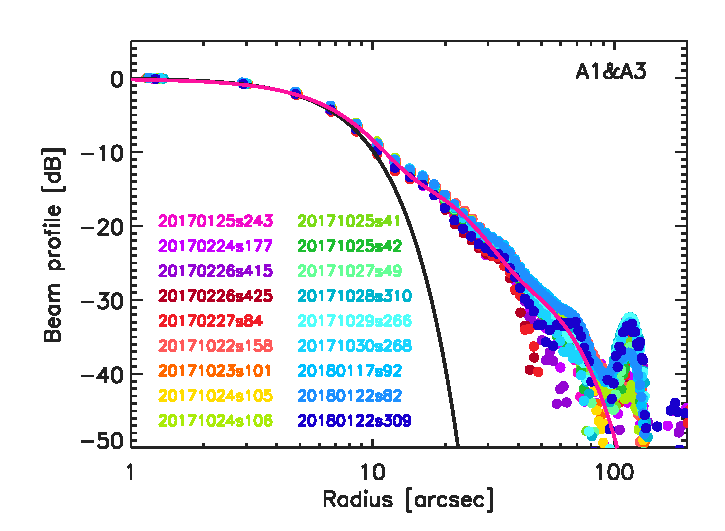
\includegraphics[clip, width=\linewidth]{Figures/plot_profiles_dB_1mm.pdf}
%   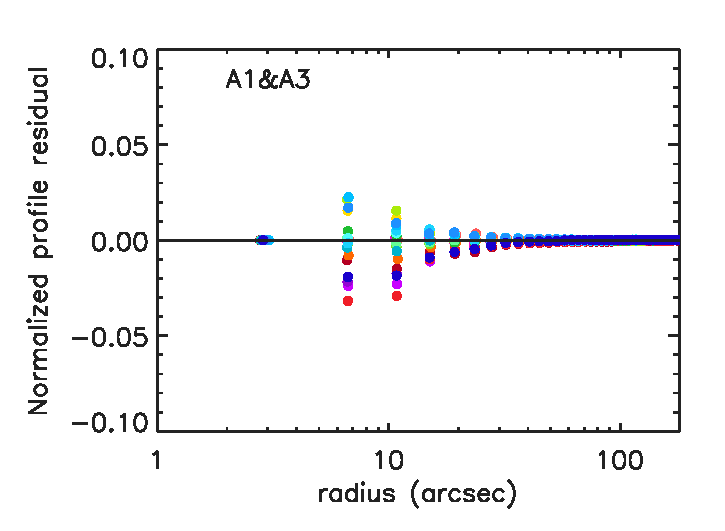
\includegraphics[clip, width=\linewidth]{Figures/plot_profile_diff_wrt_median_1mm.pdf}
   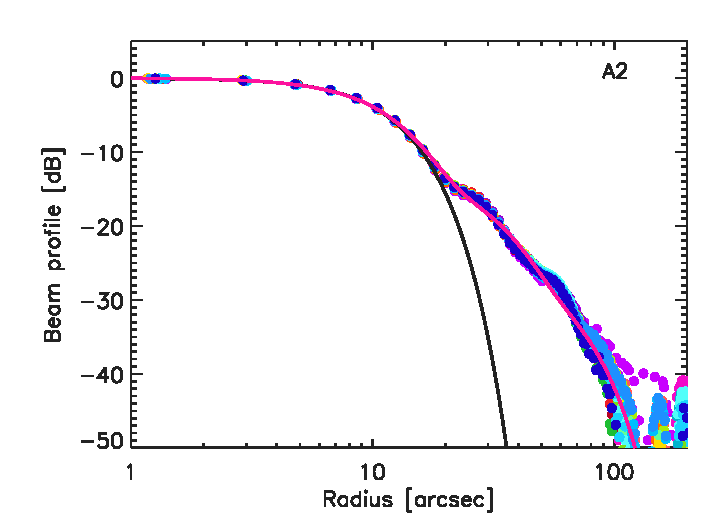
\includegraphics[clip, width=\linewidth]{Figures/plot_profiles_dB_a2.pdf}
%   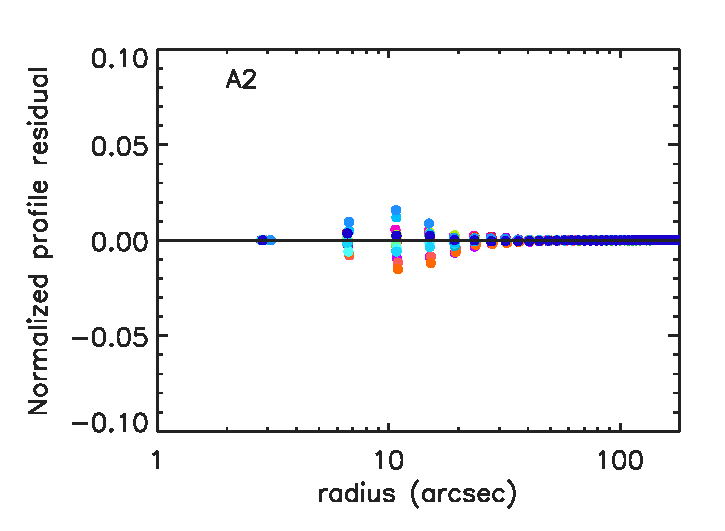
\includegraphics[clip, width=\linewidth]{Figures/plot_profile_diff_wrt_median_a2.pdf}
  \caption[Stability of the beam profile]{{\lp Beam radial
    profiles given in decibel. %as a function of the radius from the
                               %peak, given in dB.
    The data points are the beam profiles for a series of 18
    \bm\ scans acquired during the N2R8 and N2R9 commissioning campaigns and
    during the N2R12 and N2R14 science-purpose campaigns, labeled from the scan
    ID. The black line shows the main beam profile using the combined
    best-fit FWHM, as discussed in Sect.~\ref{se:mainbeam}, while the pink
    line shows the median best-fit three-Gaussian profile, as defined
    in Eq.~\ref{eq:3gauss}.}}
    %Left column plots: 
    %Beam profiles normalised to the maximum value; Right column plots:
    %difference w.r.t. the median normalised profile.
    %The radial
    %profile shapes are stable at better than $5\%$ 
    %against observing conditions.}
  \label{fig:beam_prof}
\end{figure}


%An example of the beam profile from a beam map acquired during {\emph N2R8} (scan ID:
%20170125s243)\todo{verifier le scan utilise pour les figures,
%  possibilite que ce soit 20170125s223 pris l'apres-midi}, as well as the best-fit 3-Gaussian model, is shown in
%the right panels of Fig.~\ref{fig:beam_structure_example}.

%We further fit the three-Gaussian model of Eq.~\ref{eq:3gauss} to each
%profile and gather the average best-fitting amplitudes with respect to
%the peak amplitude and FWHM in Table~\ref{tab:mean_3gauss_fit}. The
%errors are evaluated as the standard deviation of the best-fitting
%parameter values of the 18 \bm\ scans, and thus do not account for the
%correlation between parameters. These values are given to gain insight
%of the axisymmetrical pattern of the beam, but are not further used for
%the calibration. 
%
% AVERAGE 3-GAUSSIAN FIT
%\begin{table}[th]
%  \begin{center}
%    \begin{tabular}{|c|c|c|c|c|c|c|}
%      \hline
%      & \multicolumn{6}{|c|}{3-Gaussian profile parameters}  \\\cline{1-7}
%      Arrays       & Amp 1 & Amp 2 & Amp 3 & FWHM 1 & FWHM 2 & FWHM 3 \\
%      \hline\hline
%      A1        &  $0.89 \pm 0.01$   &  $0.08 \pm 0.02$  & $5 \times 10^{-3} \pm 2 \times 10^{-3}$  &  $11.0 \pm 0.2 $ & $29 \pm 2 $  & $65 \pm 15 $ \\  
%      A3        &  $0.90 \pm 0.01$   &  $0.07 \pm 0.01$  & $4 \times 10^{-3} \pm 2 \times 10^{-3}$  &  $11.0 \pm 0.2 $ & $30 \pm 3 $  & $72 \pm 23 $ \\  
%      1mm       &  $0.90 \pm 0.01$   &  $0.07 \pm 0.01$  & $4 \times 10^{-3} \pm 2 \times 10^{-3}$  &  $11.0 \pm 0.2 $ & $29 \pm 2 $  & $70 \pm 15 $ \\  
%      2mm       &  $0.96 \pm 0.01$   &  $0.3 \pm 0.3$    & $1 \times 10^{-3} \pm 0.3$ &  $17.5 \pm 0.1 $ & $63 \pm 10 $ & $65 \pm 12 $ \\  
%      \hline\hline
%    \end{tabular}
%    \caption[Average 3-Gaussian beam profile parameters]{Average
%      3-Gaussian beam profile parameters. The FWHMs are given in arcseconds.}
%    \label{tab:mean_3gauss_fit}
%  \end{center}
%\end{table}



\subsection{Main beam}
\label{se:mainbeam}

NIKA2 angular resolution {\lp is characterized by} the angular size of the main beam,
defined as the principal Gaussian (of the smaller FWHM) that encloses
most of the measured point-like source flux density.
%We have developped
%three different methods for the NIKA2 main beam characterisation
%, which are detailed
%in Sect.~\ref{se:mainbeam_methods}. Sect.~\ref{se:mainbeam_dataset}
%presents the observing scans that we have selected to derive the results
%discussed in Sect.~\ref{se:mainbeam_results}. We check the stability
%of the FWHM estimate against the observing conditions in
%Sect.~\ref{se:mainbeam_stability}.

\subsubsection{Main beam characterization methods}
\label{se:mainbeam_methods}
To characterize the main beam and to derive an estimate of the FWHM, we
have developed three methods. The two first methods, quoted
{\tt Prof-3G} and {\tt Prof-1G}, rely on a fit of the beam profile to
benefit from the signal-to-noise ratio increase after azimuthally
averaging the signal. The last one by contrast,
consists in an elliptical Gaussian fit of the beam map for a better
2D modeling, and is labeled {\tt Map-1G}. They are presented in more
detail below. \\

\noindent {\tt Prof-3G} consists in fitting the beam profile using the
three-Gaussian function defined in Eq.~\ref{eq:3gauss}.
%, and derive the FWHM from the main beam parameter.
 The main beam FWHM estimate is given by the best-fitting value
of the FWHM for the first Gaussian function.\\

\noindent {\tt Prof-1G} relies on fitting a single Gaussian to the beam
profile after masking the portion of the profile where the
contributions of the side lobes and error beams are the
largest. Specifically, the side lobe mask is designed to cut out the
radius comprized between an inner radius
$r_{\rm{in}} = 0.65\, \mathrm{FWHM}_0,$, where FWHM$_0$ is the
reference Gaussian beam FWHM (see Sect.~\ref{se:photometric_system})
and an outer radius $r_{\rm{out}} = 80''$, centered on the beam
maximum.
%At radial distances
%greater than $80''$, the profile measurement provides the base level
%for the Gaussian fit.
The profile is estimated up to a radius of
$180''$, that is in the inner part of the beam map where the noise
variance is uniform.\\

\noindent {\tt Map-1G} consists in modeling the two-dimensional distribution of
the main beam using an 2D elliptical Gaussian of size $\sigma_x$ and
$\sigma_y$. We characterize NIKA2 main beam using
\begin{equation}
  FWHM = 2 \sqrt{2\ln {2}\, \sigma_x\sigma_y}.
\end{equation}
%where $\sigma_x$ and $\sigma_y$ are the Gaussian standard deviation
%along minor and major axis.
As in {\tt Prof-1G}, we use masked versions of the
beam map to avoid side lobe and error beam contaminations. 
%The mask cuts an annulus of inner radius
%$r_{\rm{in}}$ and outer radius $r_{\rm{out}}$ centered on the beam
%maximum.
Whereas $r_{\rm{out}}$ is conservately set to be $100''$,
$r_{\rm{in}}$ is let free to vary around a central value about $8''$
for A1 and A3 and about $12''$ for A2 to provide the best 2D Gaussian
fit.

\subsubsection{Data sets for the main beam determination}
\label{se:mainbeam_dataset}

We select a sub-set of the selected \bm\ scans described in
Sect.~\ref{se:fullbeam} by discarding scans of Mars. {\lp Indeed, \bms\
toward Mars unveil the complex full beam pattern, which extends beyond
radii of $100''$, so that the annulus sidelobe mask used in {\tt
Prof-1G} and {\tt Map-1G} is not sufficient to mitigate the error
beams and sidelobes effects.}
The 12 remaining \bm\ scans are analysed using the data reduction
pipeline of Sect.~\ref{se:dataproc} and projected onto maps
with a resolution of $1''$ and an angular size of $10'$. This data set
is referred to as {\tt BM12}.

We also consider a series of shorter integration scans. We select
$5' \times 8'$ raster scans of moderately bright to very bright point
sources by thresholding the flux density estimates at $1~\rm{Jy}$ at both
wavelengths. %Slightly extended sources, such as Mars, NGC7027 and
%CRL2688 are discarded.
After the baseline scan selection, as described in
Sect.~\ref{se:data_selection}, the data set comprises 154 %163
scans towards the giant planets Uranus and Neptune, the secondary calibrator
MWC349 and the quasars 3C84, 3C273, 3C345 and 3C454 (aka
2251+158). For these short scans, which are referred to as {\tt
R154}, the data are reduced and projected onto $2''$
resolution maps. 

{\lp Finally, we use a series of 75 observation scans of Uranus and
Neptune, which includes both \bm\ and $5' \times 8'$ raster scans. 
This data set, which is referred to as {\tt UN75}, consists of all the
scans of Uranus and Neptune acquired during the N2R9, N2R12 and N2R14
observation campaigns.}


\subsubsection{Results}
\label{se:mainbeam_results}

We have derived the main beam FWHM for the three arrays and the
$1\,\rm{mm}$ arrays combination using the three methods presented in
Sect.~\ref{se:mainbeam_methods} and the data
sets of Sect.~\ref{se:mainbeam_dataset}.
%First, we test the stability of the FWHM estimates against the choices
%of the estimation method by comparing the median FWHM estimate using
%{\tt Prof 1} with the {\tt 2D beam} average FWHM from the 12 \bm\ scan
%sub-set.
Namely, our main beam FWHM estimates
consist of i) the median FWHM estimate using {\tt Prof-3G} on the
{\tt BM12} dataset, ii) the average FWHM estimate using {\tt Prof-1G}
on the {\tt UN75} data set and the {\tt Map-1G} average FWHM using
either {\tt BM12} or {\tt R154}. 
By comparing these results, we test the stability of the FWHM
estimates against the choices of the data set and of the estimation
method. %We also seek at validating the FWHM estimates using
%{\tt Prof 2}, which is further used to derive the beam efficiency in
%Sect.~\ref{se:beam_efficiency}.

In the case of Uranus, the
FWHM estimates are further corrected for the beam broadening induced
by the extension of the apparent disc. At the IRAM $30\,\rm{m}$
latitude, Uranus disc diameter varies from $3.3''$ to $3.7''$. This
induces a broadening of the Gaussian main beam of
$0.19 \pm 0.03\,\rm{arcsec}$ at $1\, \rm{mm}$ and $0.12 \pm 0.02\,\rm{arcsec}$
at $2\, \rm{mm}$. Uranus FWHM estimates are corrected for the average beam
widening values.

The results of this analysis are
gathered in Table~\ref{tab:fwhm}, including uncertainties evaluated as
the rms dispersion of single-scan based FWHM estimates.
{\tt Prof-1G} and {\tt Map-1G} results are in agreement within
uncertainties, whereas {\tt Prof-3G} yields slightly smaller FWHM.
%All the tests based on {\tt Prof 2} and {\tt 2D beam}, which both
%resort to a sidelobe mask, yield FWHM estimates
%in agreement within error bars, whereas the test using {\tt Prof 1}
%yields slightly smaller FWHM for all arrays.
%The latter provides us with lower limits for the main beam FWHM.
%The latter constitute optimistic estimates of the FWHM. 
{\lp The latter is more robust againts the error beams and large radii
beam features than the formers.}
Combined results are obtained from an error-weighted
average of the four FWHM estimates for each array.
Because the rms errors estimated using the 12 \bm\ scans may be
optimistic considering the small statistic, they are conservatively
increased to match the uncertainty estimates based on the {\tt R154}
data set before performing the weighted average.  
%The uncertainties are the most robustly derived from the dispersion of the
%best-fitting FWHM over the set of 154 OTF scans, whereas rms errors
%that are estimated from smaller and more homogeneous scan sets may be
%optimistic. Combined results are obtained from an error-weighted
%average of the four FWHM estimates for each array.
%The 12 \bm\ scan
%based rms errors were replaced by the 154 OTF scan based rms errors
%beforehand.
The combined results, as given in
Table~\ref{tab:fwhm}, provide a robust evaluation of the
FWHM. Hence, we report FWHMs of $11.1'' \pm 0.2''$ at
$1\, \rm{mm}$ and $17.6''\pm 0.1''$ at $2\, \rm{mm}$.  

\begin{table*}[!thbp]
  \caption[]{Estimates of the main beam FWHM in arcsec, using three estimation methods (see
    Sect.~\ref{se:mainbeam_methods}) and three data sets
    (see Sect.~\ref{se:mainbeam_dataset}), and their combination.}
  \label{tab:fwhm}
  \centering
  \begin{tabular}{llrrrr}
    \hline\hline
    \noalign{\smallskip}
    Method   &    Dataset   &  \multicolumn{4}{c}{FWHM ['']} \\
    \noalign{\smallskip}\cline{3-6}\noalign{\smallskip}
        &    &   A1 &  A3 & A1 $\&$ A3 &  A2  \\
    \noalign{\smallskip}
    \hline
    \noalign{\smallskip}
    {\tt Prof-3G}  &  {\tt BM12}    & $10.8 \pm 0.1$  &  $10.8 \pm 0.1$  & $10.8 \pm 0.1$  &  $17.4 \pm 0.1$  \\
    {\tt Prof-1G}  &  {\tt UN75}    & $11.3 \pm 0.4$  &  $11.2 \pm 0.4$  & $11.2 \pm 0.3$   & $17.4 \pm 0.2$  \\ 
    {\tt Map-1G}   &  {\tt R154}    & $11.3 \pm 0.2$  &  $11.1 \pm 0.2$  & $11.2 \pm 0.2$  &  $17.8 \pm 0.1$  \\ 
                   &  {\tt BM12}    & $11.2 \pm 0.1$  &  $11.1 \pm 0.1$  & $11.2 \pm 0.1$  &  $17.6 \pm 0.1$  \\
    \noalign{\smallskip}
    \hline
    \noalign{\smallskip}
    \multicolumn{2}{c}{Combined}               & $11.1 \pm 0.2$  & $11.0 \pm 0.2$  & $11.1 \pm 0.2$  &  $17.6 \pm 0.1$  \\
    \noalign{\smallskip}
    \hline
  \end{tabular}
\end{table*}

\subsubsection{Stability checks}
\label{se:mainbeam_stability}

\begin{figure}[!thbp]
\begin{center}
  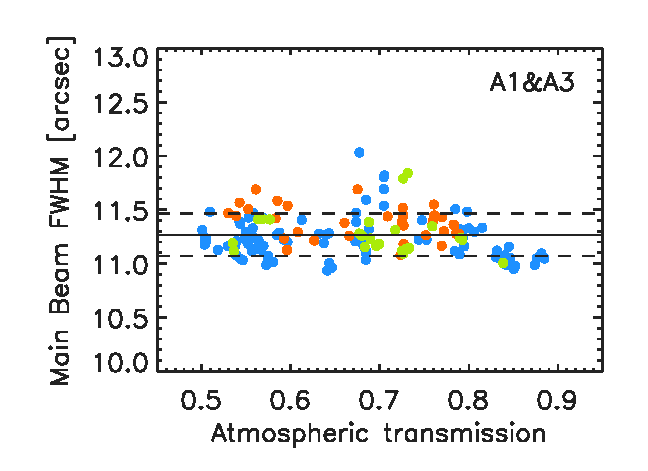
\includegraphics[clip, width=0.4\textwidth]{Figures/plot_FWHM_vs_atmtrans_mb_radius_binning2_1mm.pdf}
  \includegraphics[clip, width=0.4\textwidth]{Figures/plot_FWHM_vs_atmtrans_mb_radius_binning2_a2.pdf}
  \caption[Main Beam FWHM]{Main beam FWHM estimates for the
    $1\,\rm{mm}$ (top) and $2\,\rm{mm}$ (bottom) channels are shown as
    a function of the atmospheric transmission estimated at the
    corresponding wavelengths using bright point source observations
  acquired during N2R9, N2R12 and N2R14 campaings. }
\label{fig:fwhm_map_atmtrans}
\end{center}
\end{figure}

Figure~\ref{fig:fwhm_map_atmtrans} shows the main beam FWHM estimates
using {\tt Map-1G} as a function of atmospheric transmission,
which is modeled as $\exp{\left(-\tau \cdot x\right)}$. %, where $\tau$
%is the zenith opacity estimate and $x$ the airmass, which is
%evaluated as the cosecant of the observing elevation.
The main beam FWHM estimates using data of the three campaigns are in
agreement within rms errors. Moreover, the main beam FWHM is stable
against atmospheric conditions at both wavelengths. Slightly lower
values than average (about $11''$) are observed in the best
atmospheric conditions at $1\,\rm{mm}$ providing us with a lower limit
in the absence of correlated atmospheric noise residuals. We note
three scans acquired during the N2R12 campaign with larger FWHM than average at
$2\,\rm{mm}$ although the atmospheric transmission was excellent: this
is likely an effect of the anomalous refraction, which affected a
large number of observation scans during N2R12. 



\subsection{Beam efficiency}
\label{se:beam_efficiency}

Building upon the description of the full-beam pattern in
Sect.~\ref{se:fullbeam} and the main beam in Sect.~\ref{se:mainbeam},
we derive the beam efficiency for each array, which is defined as the
ratio of the solid angle sustained by the main beam to the total beam
solid angle.

We derive an estimate of the total beam solid angle
\begin{equation}
  \Omega_{\rm{tot}} (A_i, r_{max}) = \int_0^{r_{max}} \frac{B_{A_i}(r)}{B_{A_i}(0)} \,  2 \pi r dr
  \label{eq:omega_tot}
\end{equation}
from the normalised beam profile $B_{A_i}(r)/B_{A_i}(0)$ of the array
$A_i$ integrated up to $r_{max} = 180''$. {\lp Hereafter, we refer to
this total beam solid angle estimate as $\Omega_{180}$.}
The main beam solid angle is
evaluated from the main beam (mb) FWHM, as
$\Omega_{\rm{mb}} = 2 \pi\,  \sigma_{\rm{mb}}^2$, where FWHM$ =
2\sqrt{2\ln{2}}\, \sigma_{\rm{mb}}$. 

The choice of the maximum radius is set both by the integration depth of
the \bm\ scans, which in turn fixes the noise variance, and the
filtering due to the data processing. {\lp As discussed in
Sect.~\ref{se:dataproc}, the latter is actually targeted to the analysis of
point-like or moderately extended sources that are largely encompassed
within a $180''$-radius.}

%A large set of \bm\ scans of Uranus and Neptune acquired during the
%N2R9, N2R12 and N2R14 campaigns have been used to evaluate
%{\lp $\Omega_{180}$} from the measured beam profiles up to
%$r_{max} =180''$. %and $\Omega_{\rm{mb}}$  derived with the main beam FWHM
%estimates using the sidelobe-masked 1D method.
We evaluate {\lp $\Omega_{180}$} from the measured beam profiles
obtained using the {\tt UN75} data set (see Sect.~\ref{se:mainbeam_dataset}).
The result is given in Table~\ref{tab:solid}.

\begin{table}[!h]
\caption{Estimates of the solid angle of the total beam
  $\Omega_{180}$ given in arcsec$^{2}$ using Neptune and Uranus
  scans acquired during three observation campaigns, and the combined
  result. }
\label{tab:solid}
\centering
\begin{tabular}{l cccc}
\hline\hline
\noalign{\smallskip}
Campaigns  & \# scans & %\multicolumn{3}{c}{$\Omega_{\rm{tot}}$ (arcsec$^{2}$)} %& \multicolumn{3}{c}{$\Omega_{\rm{tot}}/\Omega_{gauss}$} \\
%\hline
%     &               &
A1    &    A2   &  A3  \\%& A1  &  A2  & A3   \\
\noalign{\smallskip}
\hline
\noalign{\smallskip}
N2R9     & 27  &  265$\pm$ 23    &  466$\pm$ 17 & 252 $\pm$ 23 \\%&  1.80 $\pm$ 0.12    &  1.35 $\pm$ 0.05   &   1.74 $\pm$ 0.13   \\
N2R12    & 20  &  229$\pm$ 11    &  437$\pm$  9 & 221 $\pm$ 10 \\%&  1.71 $\pm$ 0.06   &  1.30 $\pm$ 0.02   &   1.68 $\pm$ 0.06   \\
N2R14    & 28  &  251$\pm$ 16    &  457$\pm$ 15 & 245 $\pm$ 18 \\%&  1.73 $\pm$ 0.08   &  1.32 $\pm$ 0.03   &   1.72 $\pm$ 0.08   \\
Combined & 75  &  240$\pm$  9    &  446$\pm$  7 & 230 $\pm$  8 \\%&  1.74              &   1.32             &   1.71              \\
\noalign{\smallskip}
\hline
\end{tabular}
\end{table}

Heterodyne observations at the IRAM \trentemetre\ telescope
toward the lunar edge and the measure of forward beam efficiency using
skydips show that a non-neglectible fraction of the full beam stems
from radius greater than $180''$~\citep{Greve1998, Kramer2013}.
An accurate evaluation of the total beam solid angle would require a
dedicated observation {\lp and analysis} program to measure of the $4\pi$ integral of the
full beam pattern \citep{Greve1998, Sugimoto2004, Gusten2006}.
%This fraction is not considered here. Beam efficiency estimators that are based on
%the total solid angle estimates using Eq.~\ref{eq:omega_tot} thus
%overestimates the beam efficiency. An accurate evaluation of
%this quantity would require a dedicated observation program to measure
%of the $4\pi$ integral of the full beam pattern.
{\lp Here we use the IRAM \trentemetre\ telescope beam model described
in \citet{Kramer2013} to evaluate the beam solid angle stemming from a
radius greater than $180''$.
This quantity receives two contributions, the one of the error beams,
which are modeled as three Gaussians, and the one of the forward and
rearward spillover and scattering efficiencies. We compute the solid
angle of the main beam and error beams integrated over a radius ranging
from $180''$ to $390''$, which is the maximum radius covered by \bm\ scan,
$\Omega_{180<r<390}^{\rm{mb+eb}}$, and over radii greater
than $180''$, $\Omega_{>180}^{\rm{mb+eb}}$. The results are given in
Table~\ref{tab:solid_corr}, as well as the contribution of the forward and
rearward spillover and scattering efficiencies to the beam solid angle
$\Omega^{\rm{frss}}$. The beam solid angle integrated over $4\pi$
$Omega_{\rm{4\pi}}$ can be estimated as
\begin{equation}
\Omega_{\rm{4\pi}} = \Omega_{180} + \Omega_{>180}^{\rm{mb+eb}}
+ \Omega^{\rm{frss}}.
\label{eq:omega_beam_4pi}
\end{equation}

\begin{table}[!h]
\caption{Estimates of the various contribution to the beam solid angle
integrated up to $180''$, up to $390''$ and over $4\pi$ given in
arcsec$^{2}$. }
\label{tab:solid_corr}
\centering
\begin{tabular}{lcc}
\hline\hline
\noalign{\smallskip}
&  A1\&A3 & A2 \\
\noalign{\smallskip}
\hline
\noalign{\smallskip}
$\Omega_{180}$                  &   235 $\pm$  8 & 446 $\pm$  7 \\\noalign{\smallskip}
$\Omega_{180<r<390}^{\rm{mb+eb}}$  &   12          &   20       \\\noalign{\smallskip}
$\Omega_{>180}^{\rm{mb+eb}}$      &   21          &   41      \\\noalign{\smallskip}
$\Omega^{\rm{frss}}$             &   45          &   40      \\
\noalign{\smallskip}
\hline
\end{tabular}
\end{table}
}

We evaluate the main beam efficiencies using both the {\tt UN75} and
the {\tt BM12} data sets, as presented in
Sect.~\ref{se:mainbeam_dataset}. We compare the results based on three
estimates of the total beam and main beam solid angles: 
\begin{itemize}
  \item{{\tt BE1} relies on the best-fitting parameters of the
    three-Gaussian model of the full beam to derive the two solid
    angles. The main beam solid angle thus corresponds to the volume
    enclosed by the first Gaussian, as obtained using {\tt Prof-3G};}
  \item{{\tt BE2} consists in using $\Omega_{180}$ measurements as
    total beam solid angle estimates, while $\Omega_{\rm{mb}}$ is
    derived with the FWHM obtained using {\tt Prof-1G} (see
    Sect.~\ref{se:mainbeam_methods});}
  \item{{\tt BE3} is similar to {\tt BE2} but the main beam FWHM is
    derived using {\tt Map-1G}.}  
\end{itemize}

The beam efficiency estimates using the three methods are gathered
in Table~\ref{tab:beam_efficiency}: central values and error
bars are evaluated as the median and the rms error of the
estimates on individual \bms\ respectively. A robust evaluation of the
beam efficiency uncertainties is obtained using the rms error estimates
for {\tt BE2}, which are based on 75 \bm\ scans. We combined the
results of the three methods using an error-weighted average. Rms
errors of {\tt BE1$\&$BE3}, which rely on 12 scans, are conservatively
increased to be at least equal to {\tt BE2} rms errors beforehands.
%By contrast, error
%estimates for {\tt BE1$\&$BE3} rely on 12 scans and are thus less
%robust. We combined the results of the three methods using an error-weighted
%average. {\tt BE2} rms errors are conservatively used as a lower
%limit of the error estimates for all methods.

Using the combined results, as given in
Table~\ref{tab:beam_efficiency}, we report beam efficiencies of
$55 \pm 3 \%$ at $1\,\rm{mm}$ and  $77 \pm 2 \%$ at $2\,\rm{mm}$. 
  
%res1 = [0.54, 0.54, 0.53, 0.74]
%res2 = [0.55, 0.56, 0.55, 0.76]
%res3 = [0.59, 0.58, 0.59, 0.80]
%res = [[res1], [res2], [res3]]
%s1 = [0.03, 0.04, 0.03, 0.04]
%s2 = [0.03, 0.03, 0.03, 0.02]
%s3 = [0.07, 0.04, 0.04, 0.02]
%sig = [[s1], [s2], [s3]]
%for i = 0, 3 do print, total(res[i, *]/sig[i, *]^2)/ total(1d0/sig[i, *]^2)
%for i = 0, 3 do print, sqrt(1d0/ total(1d0/sig[i, *]^2))

\begin{table}[!h]
  \caption[]{Main beam efficiencies given in percent.}
  \label{tab:beam_efficiency}
  \centering
  \begin{tabular}{l cccc}
    \hline\hline
    \noalign{\smallskip}
    %
    %&    \multicolumn{4}{c}{Array or array combination} \\
    %\cline{2-5}
    Method & A1 &  A3 & A1 $\&$ A3 &  A2  \\
    \noalign{\smallskip}
    \hline
    \noalign{\smallskip}
    {\tt BE1}  &  $54 \pm 3$  & $54 \pm 4$  &  $53 \pm 3$  &  $74 \pm 4$  \\
    {\tt BE2} &  $55 \pm 3$  & $56 \pm 3$  &  $55 \pm 3$  &  $76 \pm 2$  \\
    {\tt BE3}&  $59 \pm 7$  & $58 \pm 4$  &  $59 \pm 4$  &  $80 \pm 1$  \\
    combined          &  $55 \pm 3$  & $56 \pm 3$  &  $55 \pm 3$  &  $77 \pm 2$  \\
    \noalign{\smallskip}
    \hline
  \end{tabular}
  %\tablefoot{ \\
  %  \tablefoottext{a}{based on {\tt Prof 3G} best-fitting parameters}
  %  \tablefoottext{b}{based on {\tt Prof 1G} main beam FWHM} 
  %  \tablefoottext{c}{based on {\tt Map 1G} main beam FWHM} 
 % }
\end{table}

%We note a
%mild improvement of the beam efficiency between the N2R9 campaign and
%the following campaigns. This could be due to the change of the method
% of setting the telescope focus:  while the focus was set at the
%best value for the center the arrays during N2R9, from N2R12
%on, the focus is set to the optimal value across the array (see the
%discussion in Sect.~\ref{}).    

\begin{table}[!ht]
\caption{Main beam efficiency estimates per observation campaigns,
given in percent.}
\label{tab:MB}
\centering
\begin{tabular}{lcccc}
\hline\hline
\noalign{\smallskip}
campaign &  A1    &    A2   &  A3    \\
\noalign{\smallskip}
\hline
\noalign{\smallskip}
N2R9    &  54.1$\pm$ 3.2   &  74.7$\pm$ 2.9  & 55.9 $\pm$ 3.7      \\
N2R12   &  55.7$\pm$ 2.0   &  77.4$\pm$ 1.0  & 57.1 $\pm$ 2.0      \\
N2R14   &  55.0$\pm$ 2.7   &  76.0$\pm$ 1.8  & 56.1 $\pm$ 2.6     \\
            %\noalign{\smallskip}
            \hline
\end{tabular}
\end{table}

As a stability check of the beam efficiency, we detail the {\tt BE2} estimates
%, as well as the level of the error beam,
for each observation campaigns, as given in Table
\ref{tab:MB}. %The level of the error beam is given relative to the
%main beam peak.%(we recall that -12dB as found is $6\%$).
We find stable beam efficiencies using observations acquired one year apart.

%\begin{table*}[!h]
%\caption{Main beam efficiency and level of error beam}
%\label{tab:MB}
%\centering
%\begin{tabular}{l| c | c c c | c c c}
%\hline\hline
%\noalign{\smallskip}
%run  & Nber of scans & \multicolumn{3}{|c|}{Main beam efficiency ($\%$)} & \multicolumn{3}{c}{Error beam level (dB)} \\
%\hline
%     &               &  A1    &    A2   &  A3    & A1  &  A2  & A3   \\
%            \hline
%N2R9    & 27  &  54.1$\pm$ 3.2   &  74.7$\pm$ 2.9  & 55.9 $\pm$ 3.7   &  -11.5 $\pm$ 0.8    &  -14.9 $\pm$ 0.6   &  -12.0 $\pm$ 0.6   \\
%N2R12   & 20  &  55.7$\pm$ 2.0   &  77.4$\pm$ 1.0  & 57.1 $\pm$ 2.0   &  -13.4 $\pm$ 0.3    &  -16.1 $\pm$ 0.3   &  -13.8 $\pm$ 0.3   \\
%N2R14   & 28  &  55.0$\pm$ 2.7   &  76.0$\pm$ 1.8  & 56.1 $\pm$ 2.6   &  -12.5 $\pm$ 0.6    &  -15.3 $\pm$ 0.6   &  -12.7 $\pm$ 0.8   \\
%            %\noalign{\smallskip}
%            \hline\hline
%\end{tabular}
%\end{table*}



%----------------------------------------------------------------------------------------
%	7./ Opacity derivation
%----------------------------------------------------------------------------------------
\section{Atmospheric opacity}
\label{se:opacity}
%----------------------------------------------------------------------------------------
%	OPACITY
%----------------------------------------------------------------------------------------
%\section{Opacity derivation}
%\label{se:opacities}
%
% LP: copie de l'intro de Xavier
In NIKA2, the opacity is measured via a total-power technique, which was successfully tested with NIKA. The details of this technique and its agreement with the Atmospheric Transmission at Microwaves (ATM) model (\cite{2001IEEE....49.1683C}) are described in \cite{Catalano2014}. The underlying idea is to replace the opacity, usually delivered by the resident IRAM tau-meter that performs elevation scans at a fixed azimuth and is operating at 225\,GHz, by a measurement that uses the NIKA2 instrument itself as a tau-meter. Using this procedure we can directly derive an opacity integrated in the NIKA2 very bandpasses and in the same line-of-sight of the source in the considered map. First, we have to calibrate the relationship between total power and opacity.
% fin copie

\subsection{Methodology}
For each kid $k$, the absolute value of the resonance frequency
$f_{tone}^k$ moves with the atmospheric load according to

\begin{equation}
f_{tone}^k = C_0^k + C_1^k T_{atm}[1-e^{-\tau/\sin\delta}]
\end{equation}

{\bf LP: pourquoi signe plus alors qu'on utilise un signe moins dans
  Eq. 2 du papier instru ?}

where $C_0^k$ is a constant equal to the resonance
frequency at zero opacity, $C_1^k$ is the calibration conversion
factor in kHz$/$K, $T_{atm}$ is the equivalent temperature
of the atmosphere (taken as a constant at 270K), $\tau$ the zenith
opacity and $\delta$ the average elevation of the telescope.
By assuming a homogeneous plane-parallel atmosphere, the airmass $x$ is defined from the
elevation as $x = \sin\delta$. 

The coefficients $C_0^k$ and $C_1^k$ are expected to be constant in time
within at least a cooldown cycle, and are determined using a {\tt
  skydip} procedure. This consists in moving
the telescope in elevation step by step and to monitor, for each kid, the
evolution of $f_{tone}^k$ vs the air mass and to fit the zenith opacity $\tau$ and
$C_0^k$ and $C_1^k$. Namely, during a {\tt skydip}, the telescope performs
eleven elevation steps in the elevation range from 19 to 65 degrees, regularly
spaced in airmass. For each step, we acquire about twenty seconds of
time traces to reduce the error in the determination of $f_{tone}^k$.

All the skydips (that were obtained under various opacity
conditions) are analysed together to break the degeneracies between
the opacity and the responsivity. The procedure has two steps.
First, all the skydips are analysed individually to simply measure
$f_{tone}^k$ for each stable elevation and fit simultaneously all the
parameters ($\tau$, $C_0^k$ and $C_1^k$.)
Error bars on $\tau$ are estimated by doing
this procedure on blocks of 40 kids only and getting a dispersion on the
resulting $\tau$ from the different blocks. Usually the dispersion comes out as
$4\times 10^{-3}$ at 1mm and $1\times 10^{-3}$ at 2mm. Once the $\tau$ values
are estimated for each skydip (as the average over the blocks), we compute
(while fixing $\tau$) the $C_0$ and $C_1$ final values for each KID. We thus
retrieve the coefficients of all the KIDs even though some of them could not
contribute to the tau determination.

%% \begin{figure}
%% \begin{center}
%% \includegraphics[clip, angle=0, scale =
%%   0.5]{Figures/NEFD_vs_tau_20170226s415_FXDC0C1_Jy_common_mode_kids_out.png}
%% \includegraphics[clip, angle=0, scale =
%%   0.5]{Figures/tau1_tau2_20170226s415_FXDC0C1_GaussPhot_common_mode_kids_out.png}
%% \caption{}
%% \label{fig:fov}
%% \end{center}
%% \end{figure}

%  figure deplacee dans Opacity_checks.tex
%\begin{figure}
%\begin{center}
%\includegraphics[clip, angle=0, scale = 0.5]{Figures/test_allskd_N2R9.jpg}
%\caption{{\bf Fix me : improve plot quality and plot only the 3rd one.}}
%\label{fig:test_allskd_N2R9}
%\end{center}
%\end{figure}

%\subsection{Opacity measurement consistency tests}

%{\bf copy from the 'Instru' paper}

\begin{figure}[ht]
\begin{center}
\includegraphics[scale=0.8]{Figures/test_allskd_N2R10v2commiss2.pdf}
\caption{Atmospheric opacity as measured from the NIKA2 data 
at 260 (top) and 150\,GHz (bottom) during N2R10
commissioning campaign. Each block of 40 KIDs gives an independent estimate of
the opacity value for each skydip scan (the integer abscissae). The block
number is the decimal value of the abscissae.
\label{fig:taumeas_paper}}
\end{center}
\end{figure}

\begin{figure}[ht]
\begin{center}
\includegraphics[scale=0.8]{Figures/test_allskd_N2R10v2commiss1.pdf}
\caption{Atmospheric opacity as measured from the NIKA2 data 
at 260 and 150\,GHz during N2R10
commissioning campaign. The error bars are in fact dispersion of the deduced
opacities between blocks of 40 KIDs.
\label{fig:taumeas_paper}}
\end{center}
\end{figure}

We observe that the skydip-fitted $\tau$ values are, as expected, common
between different detectors of the same array (the two 1mm arrays show
slightly different values). By comparing the results of different skydips, we
have verified experimentally that the coefficients $C_0$, $C_1$ are stable,
within the fit errors, on very long time scales within a cooldown cycle. The
coefficients can thus be applied to the whole observing campaign in order to
recover the opacity of each scan.


% \noindent {\bf FM : a figure would help to convince the reader that it is stable on lng time
% scale, which is a key point.}\\ FXD: I will do that figure


\begin{figure}[ht]
\begin{center}
\includegraphics[scale=0.8]{../../Paper_NIKA2_Technical/opacity_evol_run22.pdf}
\caption{Atmospheric opacity as measured from the IRAM 225\,GHz taumeter
(cyan), and from the NIKA2 data at 150 (red) and 260\,GHz (blue) during N2R9
commissioning campaign (Feb. 2017). We stress the fact that the IRAM 225\,GHz
taumeter data is not used for the atmospheric correction and is plotted here
just for comparison.
  \label{fig:taumeas_paper}}
\end{center}
\end{figure}


\begin{figure}[ht]
\begin{center}
\includegraphics[width=\linewidth]{Figures/opacity_vs_index_N2R9_N2R10.png}
\caption{Atmospheric opacity as measured from the IRAM 225\,GHz
  taumeter (black crosses), and from the NIKA2 data at 150 (red) and 260\,GHz (blue) during 
  N2R9 and N2R10 commissioning campaigns.  We stress the fact that the IRAM 225\,GHz taumeter data is not used for the atmospheric correction and is plotted here just for comparison.
  \label{fig:taumeas}}
\end{center}
\end{figure}


In Fig.~\ref{fig:taumeas} {\bf(and Fig.~\ref{fig:taumeas_paper} of
  \ref{NIKA2-Tech}) } we present the evolution of the NIKA2 in-band
opacities for all the 'OTF' scans (about 1300 scans per runs) of the
N2R9 run held in February and the N2R10 run in April 2017. These are
compared to the IRAM tau-meter values. We observe an agreement on the global trend between the IRAM tau-meter opacity
(225 GHz) and the NIKA2 values. These latter show, however,
a smaller dispersion (less than one percent).
% {\bf FM : how small ?}.


We find an average ratio between the 150 GHz and the 260 GHz NIKA2 values of
about 0.6, a bit higher than ATM model expectations. We notice however that
the 150 GHz-to-260 GHz opacity ratio varies significantly for opacities (at
150 GHz) below 0.2. This effect is likely to be linked to an $O_2$ atmospheric
line which becomes saturated or to some spillover at 2mm. This point is,
however, still under investigation.''


% \noindent {\bf FM : a figure of the ratio of taus would be useful. It should be compared with  
% Fig. \ref{thopacities}, which should appear in this section ...}
% FXD: figure above gives the measured ratio. 


\begin{figure}[ht]
\begin{center}
  \includegraphics[width=0.65\textwidth]{Figures/opacity_tau1_tau2_ratio_N2R9_N2R10.png}
  \includegraphics[width=0.65\textwidth]{Figures/opacity_tau1_tau225_ratio_N2R9_N2R10.png}
  \includegraphics[width=0.65\textwidth]{Figures/opacity_tau2_tau225_ratio_N2R9_N2R10.png}
\caption{Ratios between the 150 GHz and the 260 GHz NIKA2 zenith opacity
estimates and between the NIKA2 $\tau$ and the IRAM taumeter
values. The expectation values derived for NIKA2 bands
using the ATM model described in \ref{Pardo2002} are shown for
comparison (red and orange curves).}
  \label{fig:opacity_ratios}
\end{center}
\end{figure}

\begin{figure}[ht]
\begin{center}
  \includegraphics[width=0.8\textwidth]{Figures/opacity_tau1_tau2_byrun_ratio_N2R9_N2R10.png}
  \caption{Ratio between the 150 GHz and the 260 GHz NIKA2 zenith opacity
estimates. The expectation values derived for NIKA2 bands
using the ATM model described in \ref{Pardo2002} are shown for
comparison (red and orange curves). The observed NIKA2 opacity ratio
has a smooth, consistent behaviour over the overall probed opacity range,
and very few outlier estimates are seen although no scan selection has
been performed (out from discarding the dark tests). Also remarkable
is the consistency between estimates obtained during two campaigns
held two months apart in different weather conditions (good to average
during N2R9 and poor and often hightly unstable conditions during
N2R10). Some sub-structures are seen in the opacity ratio, which are
under investigations. They can have several origins (telescope cabin
temperature variation, variation of the $0_2$ fraction, atmospheric
temperature variation, internal temperature variations, etc).  
  }
  \label{fig:opacity_ratio_perrun}
\end{center}
\end{figure}


\begin{figure}[ht]
\begin{center}
  \includegraphics[width=0.8\textwidth]{Figures/opacity_tau1_tau2_ratio_perday_N2R9_N2R10.png}
  \includegraphics[width=0.8\textwidth]{Figures/opacity_tau1_tau2_ratio_perday_zoom_N2R9_N2R10.png}
  \caption{Ratio between the 150 GHz and the 260 GHz NIKA2 zenith
    opacity estimates. The 4 outlier estimates on February, 24 (in
    cyan) correspond to a test using the external
    calibrator. Different regimes are seen on the 25th and 26th of
    February, while the weather conditions were too unstable to allow
    the astronomer team to focus.
  }
  \label{fig:opacity_ratio_perday}
\end{center}
\end{figure}


\begin{figure}[ht]
\begin{center}
  \includegraphics[width=0.8\textwidth]{Figures/opacity_tau1_tau2_ratio_bperror10pc_N2R9_N2R10.png}
  \includegraphics[width=0.8\textwidth]{Figures/opacity_tau1_tau2_ratio_o2fraction_N2R9_N2R10.png}
\caption{Uncertainty of NIKA2 $\tau$ values. Upper panel: The impact
  of the NIKA2 transmission measurement uncertainties is illustrated
  using a very pessimistic relative uncertainty of $10\%$ (instead of
  the more realistic $1\%$ errors). Lower panel: The impact of the
uncertainty on the atmospheric absorption around $118\, \rm{GHz}$, due
to the lack of precise knowledge of the fraction of oxygene in the
atmosphere. The nominal absorption predicted by the ATM model is
modified by a factor from 0.5 to 2 in the $117-120\, \rm{GHz}$
frequency band, where the $0_2$ contributions largely dominates the
water vapor ones. }
  \label{fig:opacity_errors}
\end{center}
\end{figure}

\begin{figure}[ht]
\begin{center}
\includegraphics[width=0.9\textwidth]{Figures/opacity_tau1_tau2_emissionratio_N2R9_N2R10.png}
\caption{Ratio of the atmospheric emission in NIKA2 bands defined as
  in Eq.~\ref{eq:opacity_emission_ratio}, compared with the ATM-model
  predicted ratio calculated as in Eq.~\ref{eq:opacity_emission_ratio_model}}
  \label{fig:opacity_emission}
\end{center}
\end{figure}

The ratios between the 150 GHz and the 260 GHz NIKA2 zenith opacity
estimates, quoted $\tau_{2mm}$ and $\tau_{1mm}$ , and
between the NIKA2 $\tau$ and the IRAM taumeter values are presented in
Fig.~\ref{opacity_ratios}, along with the expectation values derived for NIKA2 bands
using the ATM model described in \ref{Pardo2002}. Namely, these
predicted values $\tau^{th}$ are calculated from the ATM-model
atmospheric zenith opacity $\tau^{ATM}$ using:  
\begin{equation}
  \tau^{th}_{A_i} = - \ln{\frac{\int e^{-\tau^{ATM}(\nu)}
      T_{A_i}(\nu) d\nu}{ \int T_{A_i}(\nu) d\nu}},
\end{equation}

where the NIKA2 bandpasses $T_{A_i}$ for arrays $A_i$, $i=1, 2, 3$, are the Martin-Pupplet reference transmissions
corrected by a Rayleigh-Jeans term  $T'_{A_i}(\nu) /
\left( \frac{\nu}{\nu_0}\right)^2$. 

In Fig.~\ref{fig:opacity_emission}, we
show the ratio of the atmospheric emission in NIKA2 bands defined as:
\begin{equation}
  R_{\rm{atm}} = \frac{1-e^{-\tau_{2mm}}}{1-e^{-\tau_{1mm}}}.
    \label{eq:opacity_emission_ratio}
\end{equation}

It is compared with the ATM-model predicted ratio
\begin{equation}
  R_{\rm{atm}}^{th} = \frac{\int (1 - e^{-\tau^{\rm{ATM}}}) T_{A_2}(\nu) d\nu }{\int T_{A_2}(\nu) d\nu} / \frac{\int (1 -
      e^{-\tau^{\rm{ATM}}}) T_{A_{1}}(\nu) d\nu }{\int T_{A_1}(\nu)
        d\nu} .
      \label{eq:opacity_emission_ratio_model}
\end{equation}

In Fig.~\ref{fig:opacity_errors}, we investigate different effects that can impact the precision with
which the zenith opacities are determined: the upper panel shows the
expected dispersion in the NIKA2 $\tau$ values coming from the transmission
measurement uncertainties: to higlight this effect, we consider a very
pessimistic relative uncertainty of $10\%$ (whereas $1\%$ would have
been a more realistic value), and the lower panel shows the impact of the
uncertainty on the fraction of oxygene in the atmosphere, which mainly 
translates in an uncertainty on the atmospheric absorption around
$118\, \rm{GHz}$: the nominal absorption predicted by the ATM model is
modified by a factor from 0.5 to 2 in the $117-120\, \rm{GHz}$
frequency band, where the $0_2$ contributions largely dominates the
water vapor ones. 



We have compared $C_0$ values, the resonance frequency at zero atmosphere,
between different runs. It appears to vary in a systematic manner. For example
we have compared N2R6 and N2R7. The change of frequencies when converted to
temperature (with $c_1$) is of about $25$ and $86$~K at 1 and $2$~mm. This
cannot be a real change of the background. Translated back by a median value
of $c_1$ ($=2500$ and $1500$~Hz/K at 1 and 2 mm), we obtain a 62.5 and 128 kHz
median downward shift of all resonant frequencies between N2R6 (October 2016)
and N2R7 (December 2016). The likely explanation is that of a slight ageing of
the KIDs. A single monolayer of oxyde could be enough to produce the downward
shift.



% LP: copie de l'intro de Xavier
In NIKA2, the opacity is measured via a total-power technique, which was
successfully tested with NIKA. The details of this technique and its agreement
with the Atmospheric Transmission at Microwaves (ATM) model
(\cite{2001IEEE....49.1683C}) are described in \cite{Catalano:2014nml}. The
underlying idea is to replace the opacity, usually delivered by the resident
IRAM tau-meter that performs elevation scans at a fixed azimuth and is
operating at 225\,GHz, by a measurement that uses the NIKA2 instrument itself
as a tau-meter. Using this procedure we can directly derive an opacity
integrated in the NIKA2 very bandpasses and in the same line-of-sight of the
source in the considered map. For that purpose, we assume that the resonance
frequency of each KID varies linearly with the total power. First, we have to
calibrate the relationship between total power and opacity. Then we can use
that calibration to measure the opacity during a given scan.
% fin copie


%----------------------------------------------------------------------------------------
%	skydip-based Method
%----------------------------------------------------------------------------------------
\subsection{Skydip-based method}
\label{se:skydip-method}

For each KID $k$, the absolute value of the resonance frequency
$f_{tone}^k$ moves with the atmospheric load according to

\begin{equation}
\ftone^k  = C_0^k - C_1^k T_{atm}[1-e^{-\tau/\sin\delta}]
\label{eq:skydip}
\end{equation}

%FXD corrected 
%{\bf LP: pourquoi signe plus alors qu'on utilise un signe moins dans
%  Eq. 2 du papier instru ?}

where $C_0^k$ is a constant equal to the resonance
frequency at zero opacity, $C_1^k$ is the calibration conversion
factor in kHz$/$K, $T_{atm}$ is the equivalent temperature
of the atmosphere (taken as a constant at 270~K), $\tau$ the zenith
opacity and $\delta$ the average elevation of the telescope.
By assuming a homogeneous plane-parallel atmosphere, the airmass $x$ is defined from the
elevation as $x = \left(\sin\delta\right)^{-1}$. 

The coefficients $C_0^k$ and $C_1^k$ are expected to be constant in
time within at least a cooldown cycle, and are determined using a {\tt
skydip} procedure. This consists in moving the telescope in elevation
step by step and monitoring, for each kid, the evolution of $\ftone^k$
versus the air mass and to fit the zenith opacity $\tau$ and $C_0^k$
and $C_1^k$. This process is realised by performing a skydip scan, as
defined in~Sect.~\ref{se:skydip}. The acquisition time spend on each
elevation step, wich is of about twenty seconds, is chosen to reduce
the error in the determination of $\ftone^k$.

All skydips, obtained under various opacity
conditions, are analysed together to break the degeneracies between
the opacity and the responsivity ($C_1^k$). The procedure has two steps.
First, all the skydips are analysed individually to simply extract
$\ftone^k$ for each stable elevation. Secondly, a simultaneous fit is done
for all 
parameters ($\tau$, $C_0^k$ and $C_1^k$.)
Error bars on $\tau$ are estimated by doing
this procedure on blocks of 40 kids only and getting a dispersion on the
resulting $\tau$ from the different blocks. Usually the dispersion comes out as
$4\times 10^{-3}$ at 1 mm and $1\times 10^{-3}$ at 2 mm. Once the $\tau$ values
are estimated for each skydip (as the average over the blocks), we compute
(while fixing $\tau$) the $C_0$ and $C_1$ final values for each KID. We thus
retrieve the coefficients of all the KIDs even though some of them could not
contribute to the $\tau$ determination.

This procedure consists thus in fitting a couple of paramaters ($C_0$,
$C_1$) for each of the several thousand valid KIDs. This requires to
have on hands a sizable amount of skydip scans -- typically ten to
twenty -- that i) span the whole opacity range and ii) avoid hightly
perturbated atmosphere to met the plane-parallel atmosphere
assumption. To that aim, we recommand to perform a skydip scan twice a
day during a scientific campagn. Then during the ($C_0$, $C_1$)
determination process, the skydip scan are thoroughtly selected.

   
\subsection{Skydip selection}


\begin{figure}[p]
\begin{center}
\includegraphics[clip=true,width=0.9\linewidth]{Figures/Opacity/plot_skydip_selection_two_crit.pdf}
\label{fig:skydip_selection}
\caption{N2R9 skydip scan selection. Median dT quality-fit criterion is plotted in fonction of Median rms criterion for each skydip scans of the N2R9 campaign and for the three arrays. Both criteria are nicely correlated. Empty diamonds show the results of the first iteration of the skydip coefficient estimation, whereas filled circled show the second iteration, for which only the skydips that met both fit-quality criteria are included. After the second iteration, all the remaining skydips met the criteria.}
\end{center}
\end{figure}

For each skydip scan and for each bunch of 40 KIDs, we compute the
difference between the measured KID resonance frequency and the model
given in Eq.~\ref{eq:skydip} taken at the best-fit values of the
($C_0$, $C_1$) parameters. Then we determine two indicators
of the fit quality per skydip. First, the standard deviation of the
measure-to-model difference is calculated over all the KIDs in a
bunch. For each skydip, we evaluate the median rms, which is the
median over the KID bunches of the standard deviation per bunch, given
in Hz. Secondly, for each scan, we compute the average
measure-to-model difference of each KID $k$, labelled $dT_k$, which is
then converted from Hertz to Kelvin using the $C_1$ parameter of the
KID $k$. Median $dT$ is the median of $dT_k$ over all the KID of an
array. With these two indicators in hands, we discard the skydip scans
that are noisy or that yield a poor fit by applying the selection
criteria

\begin{itemize}
\item Median $\rm{rms} < 1.5 \times 10^{4}~\rm{Hz}$
\item Median $dT < 1.6~\rm{K}$
\end{itemize}

The threshold values have been determined using the set of 44 skydip
scans of N2R9. The Median rms cut corresponds to twice the median of
this quantity per skydip scan, whereas the Median $dT$ cut is twice
the standard deviation of Median $dT$ over the skydips. N2R9 skydip
scan selection is illustrated in Fig.~\ref{fig:skydip_selection}, in
which the agreement between the two fit-quality criteria is clearly
seen. The ($C_0$, $C_1$) estimation proceeds in two steps: first the
parameters are estimated using all the available skydip scan for a
given campaign, then the estimation is re-iterated using the only
skydip scans that met the fit-quality criteria. After the second
iteration, we check that no extra skydip outlier are left, as shown by
the 'v2' label data points in Fig.~\ref{fig:skydip_selection}.


We test the stability of the ($C_0$, $C_1$) parameters against the exact choice of the selection criteria.  

\addparag{stability against the skydip scan selection + FIG}

At 1mm, we find about {\color{red} $[$TBC$]$  $10\%$} opacity variation from very inclusive to very aggressive selections. However, at 2mm, this scatter reachs about {\color{red} $[$TBC$]$  $30\%$} relative uncertainties.


We conclude that opacities at 1mm can be reliably estimated from a series of skydip scans using the (C0, C1) model. By contrast, for the 2mm opacities, a skydip-based method is not stable enough against the skydip selection. Thus, we adopt an hybrid approach. 

\subsection{The hybrid method}

The hybrid method comprizes two-steps: i) first the 1mm opacities,
that are $\tau_{A1}$ and $\tau_{A3}$, are determined using the skydip
method described in Sect.~\ref{se:skydip-method}, ii) then the 2mm
opacity $\tau_{A2}$ is extrapolated from the 1mm ones using a modified
ATM model. Namely, for the second step, we perform:

\begin{equation}
\tau_{A2} = \left( \left.\frac{\tau_{A2}^{\rm{ATM}}}{\tau_{A3}^{\rm{ATM}}}\right\vert_{\tau_{A3}} + \alpha \right) \tau_{A3},
\end{equation}

 where $\alpha$ is an offset, which are estimated from the observations themselves, and the ratio is the predicted zenith opacity ratio for A2 and A3 frequency bands using the ATM model described in \ref{Pardo2002} and taken at the measured A3 zenith opacity. The zenith opacity expectations for the array $A_i$ is
\begin{equation}
  \tau^{\rm{ATM}}_{A_i} = - \ln{\frac{\int e^{-\tau^{ATM}(\nu)} T_{A_i}(\nu) d\nu}{ \int T_{A_i}(\nu) d\nu}},
\end{equation}
where the bandpasses $T_{A_i}$ for arrays $A_i$, $i=1, 2, 3$, are the Martin-Pupplet reference transmissions
corrected by a Rayleigh-Jeans term  $T'_{A_i}(\nu) / \left( \frac{\nu}{\nu_0}\right)^2$. 

We observe that the measured \emph{shape} of the measured opacity ratio is well described by the ATM expectations whereas its \emph{amplitude} is too low by an offset $\alpha$, which we dertermine using a data-driven approach. We estimate $\alpha$ as the offset that ensures a stability of the A2 flux over the whole opacity span.  

\addparag{$\alpha$ fit + FIG}





%----------------------------------------------------------------------------------------
%	Tests
%----------------------------------------------------------------------------------------
\subsection{Baseline opacity measurements}

%{\bf copy from the 'Instru' paper}

%\begin{figure}[ht]
%\begin{center}
%\includegraphics[scale=0.8]{Figures/test_allskd_N2R10v3commiss2.pdf}
%\caption{Atmospheric opacity as measured from the NIKA2 data 
%at 260 (top) and 150\,GHz (bottom) during N2R10
%commissioning campaign. Each block of 40 KIDs gives an independent estimate of
%the opacity value for each skydip scan (the integer abscissae). The block
%number is the decimal value of the abscissae.
%\label{fig:taumeas_paper}}
%\end{center}
%\end{figure}

%\begin{figure}[ht]
%\begin{center}
%\includegraphics[scale=0.8]{Figures/test_allskd_N2R10v2commiss1.pdf}
%\caption{Atmospheric opacity as measured from the NIKA2 data 
%at 260 and 150\,GHz during N2R10
%commissioning campaign. The error bars are in fact dispersion of the deduced
%opacities between blocks of 40 KIDs.
%\label{fig:taumeas_paper}}
%\end{center}
%\end{figure}

We observe that the skydip-fitted $\tau$ values are, as expected, common
between different detectors of the same array. By comparing the results of different skydips, we
have verified experimentally that the coefficients $C_0$, $C_1$ are stable,
within the fit errors, on very long time scales within a cooldown cycle. The
coefficients can thus be applied to the whole observing campaign in order to
recover the opacity of each scan.


% \noindent {\bf FM : a figure would help to convince the reader that it is stable on lng time
% scale, which is a key point.}\\ FXD: I will do that figure


\begin{figure}[ht]
\begin{center}
\includegraphics[scale=0.8]{../../../Paper_NIKA2_Technical/opacity_evol_run22.pdf}
\caption{Atmospheric opacity as measured from the IRAM 225\,GHz taumeter
(cyan), and from the NIKA2 data at 150 (red) and 260\,GHz (blue) during N2R9
commissioning campaign (Feb. 2017). We stress the fact that the IRAM 225\,GHz
taumeter data is not used for the atmospheric correction and is plotted here
just for comparison.
  \label{fig:taumeas_paper}}
\end{center}
\end{figure}


\begin{figure}[ht]
\begin{center}
\includegraphics[width=\linewidth]{Figures/opacity_vs_index_N2R9_N2R10.png}
\caption{Atmospheric opacity as measured from the IRAM 225\,GHz
  taumeter (black crosses), and from the NIKA2 data at 150 (red) and 260\,GHz (blue) during 
  N2R9 and N2R10 commissioning campaigns.  We stress the fact that the IRAM 225\,GHz taumeter data is not used for the atmospheric correction and is plotted here just for comparison.
  \label{fig:taumeas}}
\end{center}
\end{figure}


In Fig.~\ref{fig:taumeas} {\bf(and Fig.~\ref{fig:taumeas_paper} of
  \ref{NIKA2-Tech}) } we present the evolution of the NIKA2 in-band
opacities for all the 'OTF' scans (about 1300 scans per runs) of the
N2R9 run held in February and the N2R10 run in April 2017. These are
compared to the IRAM tau-meter values. We observe an agreement on the global trend between the IRAM tau-meter opacity (225 GHz) and the NIKA2 values. These latter show, however,
a smaller dispersion (less than one percent).




%----------------------------------------------------------------------------------------
%	8./ Calibration
%----------------------------------------------------------------------------------------
\section{Calibration}
\label{se:calibration}
%----------------------------------------------------------------------------------------
%	8./ Calibration
%----------------------------------------------------------------------------------------
%\section{Calibration}
%\label{se:calibration}

In this section, we present the absolute calibration of the flux densities. We
use Uranus as the main primary calibrator. Sect.~\ref{se:calibration_method}
describes the absolute calibration method, Sect.~\ref{se:flat_field} presents
the inter-calibration of all the KIDs and the flat fields. While
gathering several observations of calibrators, we have evidenced a
daily variation of the absolute calibration
coefficients related to daily variation of the beam
size induced by weather temperature. If left uncorrected, it leads to
a sizeable increase of the calibration uncertainties. To
overcome this issue, we primarily flag the most impacted observation
times of the day and exclude them from further analysis.
%while not being strictly related to the instrument.
We discuss this effect in
Sect.~\ref{se:beam_variation}. In Sect.~\ref{se:baseline_calibration},
the \emph{baseline} calibration procedure is summarized and stability
tests are performed.  

%%  In short, as
%% a first step, {\lp an absolute calibration factor per detector} is derived using
%% a \bm\ scan of Uranus. This step determines also the inter-calibration of all
%% the KIDs. In a second step, the flux density absolute scale is further refined
%% by monitoring the primary calibrator all along the observation campaign to
%% estimate {\lp a corrective rescaling of the absolute calibration
%%   factor}. Section~\ref{se:calibration_method} describes the absolute
%% calibration method. Section~\ref{se:flat_field} presents the inter-calibration
%% and the flat fields. While monitoring the calibrator fluxes along observation
%% runs in order to improve and test the stability of our calibration, we have
%% evidenced a daily variation of the absolute calibration coefficients related to
%% external temperature-induced variation of the beam size. If left uncorrected,
%% this variation leads to a sizable increase of the calibration uncertainties
%% while not being strictly related to the instrument. To overcome this issue, we
%% primarily flag the most impacted observation times of the day and exclude them
%% from further analysis. We resort to this conservative approach in the
%% \emph{baseline} calibration method, as discussed in
%% Sect.~\ref{se:data_selection}. In appendix~\ref{se:photometric_correction}, we
%% present an approach that partly mitigates this effect.
%% 
%% First we describe the method for the absolute calibration in
%% Sect.~\ref{se:calibration_method}, then we present the inter-calibration and the
%% flat fields in Sect.~\ref{se:flat_field}. Finally, the baseline calibration is
%% presented in Sect.~\ref{se:baseline_calibration}.
%% 
%% %% The temperature-induced variation and the
%% %% beam size monitoring are then discussed in
%% %% Sect.~\ref{se:beam_variation}.
%% %% 
%% %%  and the calibration
%% %% with a photometric correction in
%% %% Sect.~\ref{se:photometric_correction}.  


%---------------------------------------------------------------------
%	Method
%---------------------------------------------------------------------

\subsection{Absolute calibration procedure and photometric system}
\label{se:calibration_method}

We detail here the procedure for calibrating the absolute scale of
the flux density and the chosen photometric system.

\subsubsection{Photometric system}
\label{se:photometric_system}

The main primary calibrators of NIKA2 are the giant planets Uranus and
Neptune. The latter is used when the former is not visible in the most
stable observing conditions. The flux density expectations of the
primary calibrators are derived in Appendix~\ref{ap:ref_flux_calibrator}. 
%
\begin{table}[!htbp]
\caption{NIKA2 reference frequencies and FWHM}
\label{tab:definitions}
\centering     
\begin{tabular}{lcc}
\hline\hline
      \noalign{\smallskip}
      & 1 mm & 2 mm \\
      \noalign{\smallskip}
      \hline
      \noalign{\smallskip}
      Reference frequency, $\nu_{0}$ & 260 GHz & 150 GHz \\
      Reference FWHM,  FWHM$_{0}$    & 12.5'' & 18.5'' \\
      \noalign{\smallskip}
      \hline
\end{tabular}
\end{table}

We parametrize the primary calibrator flux density as 
$S_{\rm{c}}(\nu) = S_{\rm{c}}(\nu_0)\, f(\nu/\nu_{0})$, where $f(\nu/\nu_{0})$
encloses the spectral dependence, 
as a function of a reference frequency $\nu_{0}$ that we choose
arbitrarily to be: $\nu_{0} = 150$~GHz for the $2\,\rm{mm}$ array and
$\nu_{0}= 260$~GHz for both $1\,\rm{mm}$ arrays. After projecting the raw
data (in units of the KID resonance frequency shift, $\rm Hz$) of a
calibrator {\sl c} on the sky, we model the calibrator raw map as a
fixed-width 2D Gaussian
%\begin{equation}
%  R_{\rm{c}}(\theta, \phi)  = \frac{A_{\rm{c}}}{2 \pi \sigma_{0}^{2}}
%  e^{-\frac{\theta^{2}}{2\sigma_{0}^{2}}},
%  \label{eq:gaussian_amplitude}
%\end{equation}
\begin{equation}
  R_{\rm{c}}(\theta, \phi)  = A_{\rm{c}} \, e^{-\frac{\theta^{2}}{2\sigma_{0}^{2}}},
  \label{eq:gaussian_amplitude}
\end{equation}
{\lp where $A_{\rm{c}}$ is the amplitude of the 
Gaussian in Hz,} and $\sigma_{0}$ is derived from the
reference FWHM, labelled FWHM$_{0}$, which is $12.5''$ for the $1\, \rm{mm}$
arrays and $18.5''$ for the $2\,\rm{mm}$ array. These values have
been chosen larger than the main beam values, as reported in
Sect.~\ref{se:beam}, to account for a fraction of the signal stemming from
the first error beam and first side lobes.
Both the reference frequency, $\nu_0$, and the reference FWHM, FWHM$_{0}$, define
our reference photometric system, as summarized in Table~\ref{tab:definitions}.

The absolute calibration coefficients are estimated from observations
of primary calibrators $c$, as the ratio of
the calibrator flux density expectations at the reference frequency
$S_{\rm{c}}(\nu_0)$ and $A_{\rm{c}}$. Then, for any observed point-like source
{\sl s} of projected map $R_{\rm{s}}(\theta,\phi)$ in Hz, the map
\begin{equation}
  M_{\rm{s}}(\theta, \phi) = \frac{S_{\rm{c}} (\nu_{0})}{A_{\rm{c}}}
  R_{\rm{s}}(\theta,\phi),
  \label{eq:pointsourcephot}
\end{equation}
is calibrated in Jy/beam. {\lp The best-fit amplitude estimate
of the fixed-width FWHM$_{0}$ Gaussian on this map directly gives an
estimate of the flux density of the source at the reference
frequency $S(\nu_{0})$, excluding colour corrections.}
%as
%\begin{equation}
%S(\nu_{0})  = \frac{S_{\rm{c}}(\nu_{0})}{A_{\rm{c}}} \, A_{\rm{s}},
%\label{eq:pointsourcephot}
%\end{equation}
%where $A_{\rm{s}}$ is the amplitude estimate from the raw map.

\begin{table*}[!thbp]
\caption{Colour correction factors for a target source  $S \propto \nu^{\alpha_{\rm{s}}}$, as defined using Eq.~\ref{eq:color_correction}.}
\label{tab:mod}
\centering 
\begin{tabular}{lrrrrrrrr}
\hline\hline
\noalign{\smallskip}
Array     & \multicolumn{8}{c}{$\alpha_{\rm{s}}$} \\
\noalign{\smallskip}
\hline
\noalign{\smallskip}
         &  -2 &  -1    &    0  & + 0.6 & +1  &  +2  & +3 & +4  \\       
\noalign{\smallskip}
\hline
\noalign{\smallskip}
          A1   & 0.876  &  0.916   &   0.951  & 0.969 &  0.981   &  1.005  &    1.024  &  1.037   \\
          A2   & 0.945  &  0.972   &   0.990  & 0.996 &  0.998   &  0.997  &    0.986  &  0.966      \\ 
          A3   & 0.907  &  0.940   &   0.967  & 0.980 &  0.987   &  1.001  &    1.009  &  1.011     \\
            \noalign{\smallskip}
            \hline
\end{tabular}
\end{table*}

\subsubsection{Colour correction}

The flux density estimate $S(\nu_{0})$ gives the
flux of the source at the reference frequency only if the source has
the same spectral behaviour as the calibrator. In general, to retrieve the
flux of the source at the reference frequency, a colour correction
$C_{\rm{s}}$ has to be applied
\begin{equation}
S_{\rm{s}}(\nu_{0}) = S(\nu_{0}) \,  C_{\rm{s}}(\nu_{0}, I_\nu^{\rm{s}}),
\end{equation}
which depends on the reference frequency $\nu_{0}$, the source
SED $I_\nu^{\rm{s}}$ and the NIKA2 bandpasses.
Neglecting the effect of the atmosphere on the NIKA2 transmission, we
compute the colour correction factor for target sources of SED that are
different from Uranus using
\begin{equation}
  C_{\rm{s}}(\nu_{0}, I_\nu^{\rm{s}}) = \frac{\int_{0}^{+\infty} I_\nu^{\rm{c}}~T({\nu})\, d\nu}{ \int_{0}^{+\infty} I_\nu^{\rm{s}}~ T({\nu})\, d\nu},
    \label{eq:color_correction}
\end{equation}
where $T({\nu})$ is the NIKA2 transmission
(Sect.~\ref{se:instru_bandpass}).
Assuming Rayleigh-Jeans SED for the calibrator
($I_\nu^{\rm{c}} \propto (\nu/\nu_0)^{\alpha_{\rm{c}}}$) and the source
($I_\nu^{\rm{s}} \propto (\nu/\nu_0)^{\alpha_{\rm{s}}}$), and a
spectral index $\alpha_{\rm{c}} = 1.6$ for Uranus, we provide colour
correction factors for eight values of the spectral index of the
source $\alpha_{\rm{s}}$ in Table~\ref{tab:mod}.


\subsubsection{Extended sources}
\label{se:extended_source_calib}

%{\rev For the sake of studying the diffuse emission or
%performing aperture photometry, maps given in Jy/beam units, which
%are a relevant system of units for point sources, need to be converted
%in Jy/sr.}
{\rev While study of point sources are usually performed with maps given in
Jy/beam unit, diffuse emission studies or aperture photometry ones
require map expressed in Jy/sr. To that aim, we need to take into
account the full beam pattern, as discussed in Sect.~\ref{se:beam_efficiency}.}
%{\lp The Jy/beam units map $M_{\rm{s}}(\theta, \phi)$ can not be used
%directly to perform aperture photometry or to obtain the flux density
%of extended sources. We first need to convert
%$M_{\rm{s}}(\theta, \phi)$ in a map in Jy/sr,
%$M_{\rm{ap}}(\theta, \phi)$, taking into account the full beam
%pattern, as discussed in Sect.~\ref{se:beam_efficiency}. 
First we correct with the solid angle enclosed in the
reference fixed-width Gaussian beam $\Omega_{0} = 2\pi \sigma_0^2$ to
obtain a map homogeneous to Jy/sr. Then, to account for the signal in
the total beam pattern, we further correct with the reference beam
efficiency BE$_{0}$. As defined as the ratio of $\Omega_{0}$ and the
total beam solid angle $\Omega_{\rm{tot}}$, BE$_{0}$ represents the
fraction of the full beam solid angle that is enclosed in the solid
angle sustained by the reference beam. To summarize, the map in Jy/sr
$M(\theta, \phi)$ relates to the map in Jy/beam
$M_{\rm{s}}(\theta, \phi)$ using
%
\begin{equation}
M(\theta, \phi) = \frac{\rm{BE}_{0}}{\Omega_{0}} \, M_{\rm{s}}(\theta, \phi).
\label{eq:jybeam_to_jysr}
\end{equation}
%
\begin{table}[!htbp]
  \caption[]{Reference beam efficiencies for Array 1, Array 3, Array 1\&3 and Array 2}
  \label{tab:reference_beam_efficiency}
  \centering    
  \begin{tabular}{lrrrr}
    \hline\hline
    \noalign{\smallskip}
    & A1 & A3  & A1\&3 & A2 \\
    \noalign{\smallskip}
    \hline
    \noalign{\smallskip}
    FWHM$_{0}$ [arcsec]          & $12.5$     &  $12.5$     & $12.5$     & $18.5$     \\
    BE$_{0}$   [\% ]             & $60 \pm 3$ &  $61 \pm 3$ & $61 \pm 3$ & $72 \pm 2$ \\
        \noalign{\smallskip}
    \hline
  \end{tabular}
\end{table}
%
{\rev In Table~\ref{tab:reference_beam_efficiency}, we provide the
estimates of the reference beam efficiency, which are derived from the
measured $\Omega_{\rm{tot}}$ as given in
Sect.~\ref{se:beam_efficiency}.}
%Propagating the uncertainty on the
%total beam solid angles, the reference beam efficiencies are estimated
%with a precision of 10$\%$ and 6$\%$ at 1 and 2\,mm
%respectively. These uncertainties must be accounted for in the error
%budget after conversion of the maps from Jy/beam to Jy/sr units.}


%{\lp
%In Table~\ref{tab:reference_beam_efficiency}, we provide the reference
%beam efficiencies estimated up to a radius of $180''$, which are
%computed as the ratio between $\Omega_{0}$ and
%$\Omega_{180}$ (see Sect.~\ref{se:beam_efficiency}). To account for the power stemming from radii
%ranging from $180''$ to a cutting radius $r_{\rm{c}}$, we estimate 
%correcting factors $\eta_{r_{\rm{c}}}$ to these reference beam
%efficiencies, defined as  
%\begin{equation}
%\eta_{r_{\rm{c}}} = \left( 1 + \frac{\Omega_{180<r<r_{\rm{c}}}}{\Omega_{180}} \right)^{-1}.
%\end{equation}
%We give the correcting factor $\eta_{390}$ accounting for the main
%beam and error beams contributions up to $6.5'$
%using $\Omega_{180<r<390}^{\rm{mb+eb}}$, as given in
%Table~\ref{tab:solid_corr}, as well as the correcting factor
%$\eta_{\rm{tot}}$ accounting for the total beam
%solid angle using Eq.~\ref{eq:omega_beam_4pi}. These correcting
%factors are given in Table~\ref{tab:reference_beam_efficiency}.
%}

%\begin{table}[!htbp]
%  \caption[]{Reference beam efficiencies for Array 1, Array 3, Array
%    1\&3 and Array 2}
%  \label{tab:reference_beam_efficiency}
%  \centering    
%  \begin{tabular}{lrrrr}
%    \hline\hline
%    \noalign{\smallskip}
%    & A1 & A3  & A1\&3 & A2 \\
%    \noalign{\smallskip}
%    \hline
%    \noalign{\smallskip}
%    FWHM$_{0}$ [arcsec]          &  $12.5$   &  $12.5$  &   $12.5$  &   $18.5$  \\
%    BE$_{0}$\tablefootmark{a}\hspace{3mm}  [\% ] & $70 \pm 4$ & $72 \pm 4$ & $70 \pm 4$ & $85 \pm 3$ \\
%    \noalign{\smallskip}
%    $\eta_{390}$\hspace{3mm}  & $0.95$ & $0.95$ & $0.95$ & $0.96$ \\
%    $\eta_{\rm{tot}}$\hspace{3mm}  & $0.78$ & $0.78$ & $0.78$ & $0.85$ \\
%    \noalign{\smallskip}
%    \hline
%  \end{tabular}
%  \tablefoot{ \\
%    \tablefoottext{a}{Reference Beam Efficiency, estimated as the ratio between the reference FWHM beam power and the total beam power up to a radius of 180 arcsec} 
%  }
%\end{table}


\subsubsection{Calibration procedure}
\label{se:practical_calib}

{\lp In practice, the calibration procedure is performed in two steps. First
$S_{\rm{c}}(\nu_{0})$-to-$A_{\rm{c}}$ ratios per detector $G_k$
are estimated for each KID $k$ using the map per KID projected from
a \bm\ scan of a calibrator. The calibration coefficient $G_k$
for the KID $k$ is computed at zero atmospheric opacity as:
\begin{equation}
  G_k = \frac{S_{\rm{c}}(\nu_0)\, e^{-\taunu\,x}}{A_k},
  \label{eq:kid_gain}
\end{equation}
where $S_{\rm{c}}(\nu_0)$ is the expected flux density of the source at
the reference frequency $\nu_0$ (see
Appendix~\ref{se:ref_flux_uranus_neptune}), $\taunu\, x$ is the
line-of-sight opacity measured using the {\tt corrected skydip} method
(see Sect.~\ref{se:opacity}) and $A_k$ is the best-fit
amplitude of the reference FWHM$_0$ Gaussian, which is fitted in the
KID map. % using Eq.~\ref{eq:gaussian_amplitude}.
This first step accounts for both the relative calibration between KIDs and the absolute
calibration using a single calibrator scan.

Secondly, the absolute calibration is further refined by evaluating a
flux density rescaling factor using a series of observations of
Uranus or Neptune. After the first step of the calibration is
performed, the KID TOI are projected into a calibrated map $M_\nu$, as
described in Sect.~\ref{se:dataproc}, where $\nu$ stands for the three
arrays and the $1\,\rm{mm}$-array combination, and the atmospheric attenuation
is corrected. For each of the calibrator observation scans, we
compute the ratio between the expected calibrator flux density
$S_{\rm{c}}(\nu_{0})$ and the measured calibrator flux density in $M_\nu$, which
is estimated as described in Sect.~\ref{se:photometric_system}. The
flux density rescaling factor per array is the average
expected-to-measured flux density ratio over all the selected calibrator scans.} 

%the absolute calibration consists in evaluating a flux
%density rescaling factor using a series of OTF scans toward
%Uranus or Neptune. This flux rescaling factor is an estimate of the
%$S_{\rm{c}}(\nu_{0})$-to-$A_{\rm{c}}$ ratio of Eq.~\ref{eq:pointsourcephot}. The
%expected calibrator flux density $S_{\rm{c}}(\nu_{0})$ is obtained as
%discussed in Appendix~\ref{se:ref_flux_uranus_neptune}, whereas the measured
%amplitude $A_{\rm{c}}$ is estimated as the average amplitude of the FWHM$_0$
%Gaussian fitted from a series of calibrator maps.
%
%Before the flux density estimation, the calibrator raw data are i)
%intercalibrated as decribed in Sect.~\ref{se:flat_field} and ii) corrected for the
%atmospheric attenuation as described in Sect.~\ref{se:opacity}. To
%refine the intercalibration between the two $1$-mm arrays after the
%KID Hertz to Jy/beam conversion factor estimates, a flux rescaling
%factor per array is calculated.

The primary calibrator scans are first selected as discussed in
Sect.~\ref{se:data_selection}. Then, in addition to
the \emph{baseline} scan selection cuts, we use a Gaussian beam size
criterion. The FWHM estimated from the planet
observation map is required to be lower than $12.5''$ at $1\,\rm{mm}$ and lower
than $18''$ at $2\,\rm{mm}$. In further mitigating the flux scatter
due to beam broadening, we ensure better accuracy of the absolute
calibration.



%---------------------------------------------------------------------
%	INTERCALIBRATION
%---------------------------------------------------------------------
\subsection{Relative calibration \& flat fields}
\label{se:flat_field}
While absolute calibration of each KID also \emph{de facto} provides
relative calibration, the latter is interesting in itself to
characterize the instrument. We focus on this aspect in this
section.

\begin{figure*}[!thbp] 
\begin{center}
  \includegraphics[width=0.95\textwidth]{Figures/Average_main_beam_flat_field_N2R9_10.png}
  \includegraphics[width=0.8\textwidth]{Figures/Histo_average_main_beam_flat_field_N2R9_10.png}
\caption[Average main beam flat fields]{Average main beam flat fields
  obtained by combining the flat fields of five
  \bm\ scans. The top row plots show the normalized average flat fields of Array
  1, 3 and 2, respectively. {\lp The offset positions with respect to the center of
  the array are given in arcsecond in the Nasmyth coordinate
  system. The colour code gives the value of the KID calibration
  coefficients, as defined in Eq.~\ref{eq:kid_gain}, normalized by the
  average calibration coefficient over all the
  KIDs of the array.} The bottom plots
  show the average flat field distributions using all KIDs (blue),
  using Array 1 KIDs that are positioned out of the shadow zone
  (green) and using Array 1 KIDs inside the shadow zone, which is
  defined in the text.}
 \label{fig:avg_mbff}
\end{center}
\end{figure*}

The dispersion of the detector responsivity across the field of view (\aka\ flat
fields) has been characterized in the following ways.

\noindent \emph{Main beam flat fields.} These are the focal plane
distribution of the calibration coefficients per KID. {\lp They describe the
focal plane distribution of the point spread function (PSF) in
the far field of the telescope.} The calibration coefficients $G_k$ are
estimated using Eq.~\ref{eq:kid_gain}, as discussed in
Sect.~\ref{se:practical_calib}. 

\noindent \emph{Forward beam flat fields.} These are the focal plane
distributions of the relative response of
each KID to the near field atmospheric background. They are estimated
using the correlation factor of each detector TOI 
to a median common mode estimated off-source (see Sect.~\ref{se:toi_proc} for
more details on common modes).

Figure~\ref{fig:avg_mbff} %and \ref{fig:avg_fbff}
shows the average main beam %and forward beam
flat field for the three arrays. These have been constructed by
combining the normalized flat fields of five \bms\ acquired during two
technical observation campaigns. These data were
selected by thresholding the line-of-sight opacity measured in the
1\,mm band to $\taunu\,x \leq 0.85$. The distributions for the average flat
fields are shown in the bottom panel of Fig.~\ref{fig:avg_mbff}.% and \ref{fig:avg_fbff}.

We observe a significant variation of the flat fields for A1 from the left-most side
to the right-most side of the FOV. This reveals a significant change of A1
detector responsivities depending on their position in the focal plane. Namely, this
effect mainly impacts the left-most third of the array, which is
referred to as the "shadow-zone''. This variation of the
flat field translates into a broadening of the distribution shown in
the lower panel of Fig.~\ref{fig:avg_mbff}.  However,
we verified that A1's flat field dispersions are in line with the ones of A3 after the
detectors within the shadow-zone were flagged out using a
crescent-shaped mask. The masked flat field distributions are shown in
green in Fig.~\ref{fig:avg_mbff}, %and \ref{fig:avg_fbff}
whereas shadow-zone distributions are in red. The same FOV patterning
is also observed in the forward beam flat fields, which excludes a
main beam related issue. 

%In addition to the average flat fields, we further
%characterize the flat fields for individual \bms. Fig.~\ref{fig:stddev_ff}
%shows the dispersion of the flat fields for nine \bms\ using
%either the whole FOV or masking the shadow-zone. The dispersion estimates for
%this two cases are gathered in Table~\ref{tab:flatfield_res}.
%While the
%shadow zone is exluded, the A1 flat field dispersions are reduced by a
%factor of about two, and reached values close to that of the A3 flat
%field dispersions, while the latters are unchanged. 

%\begin{table}[!h]
%\begin{center}
%\begin{tabular}{|l|l|c|c|c|}
%\hline
% Dispersion ($\%$)    & KID selection  &  A1 & A3  & A2 \\
%\hline
%Main beam flat field  & all the FOV           & $34.4 \pm 3.4$    & $15.5 \pm 1.4$  &  $13.2 \pm 1.7$  \\
%                      & shadow-zone excluded  & $17.0 \pm 1.1$    & $14.2 \pm 1.2$  &  $12.8 \pm 1.3$\\
%\hline
%Forward beam flat field  & all the FOV           & $21.6 \pm 1.4$  & $10.1 \pm 1.7$  & $5.2 \pm 0.9$   \\
%                         & shadow zone excluded  & $12.2 \pm 1.6$  & $10.1 \pm 2.1$  & $4.9 \pm 1.2$ \\
%\hline
%\end{tabular}
%\caption[Flat field dispersions]{Average flat field dispersions in percent for
%  nine \bms\ over all the FOV and after masking out the shadow-zone}
%\label{tab:flatfield_res}
%\end{center}
%\end{table}

%\begin{figure*}[!thbp] 
%\begin{center}
%  \includegraphics[width=0.95\textwidth]{Figures/Average_near_beam_flat_field_N2R9_10.png}
%  \includegraphics[width=0.8\textwidth]{Figures/Histo_average_near_beam_flat_field_N2R9_10.png}
%\caption[Average forward efficiency flat fields]{Average forward efficiency flat field for array 1, 3 and
%  2. Same legend as Fig.~\ref{fig:avg_mbff}}
% \label{fig:avg_fbff}
%\end{center}
%\end{figure*}

%\begin{figure}[ht] 
%\begin{center}
%  \includegraphics[width=0.6\textwidth]{Figures/FlatFields/Dispersion_main_beam_flat_field_N2R9_10_.png}
%  \includegraphics[width=0.6\textwidth]{Figures/FlatFields/Dispersion_forward_beam_flat_field_N2R9_10_.png}
%\caption[Dispersion of the flat field for nine \bms.]{The RMS
%  dispersion of the normalised main beam flat field (upper panel) and forward beam flat
%  field (lower panel) are shown using all valid KIDs of Array 1 (red circles),
%  Array 3 (orange circles) and Array 2 (blue circles), and using the KIDs
%  located outside the Array 1 "shadow zone'', which was discarded using a left
%  crescent-shaped mask (red crosses).}
% \label{fig:stddev_ff}
%\end{center}
%\end{figure}

The shadow zone effect is caused by {\lp a misbehaving of the dichroic in
the polarized transmission which is out of specifications. As a
result, the $1\,\rm{mm}$ polarisation that illuminates A1 is
attenuated.}
This effect,
which implies %a wrong placement of the transition zone of the dichroic
%that depends on frequency, incidence angle and polarisation,
{\lp a dependence of the frequency cut-off on the radiation
incidence angle and linear polarisation,}
was reproduced using optical simulations. Furthermore, this hypothesis was
verified using observations at the technical campaign of September
2018. During this test campaign, a new \emph{hot-pressed} dichroic had
been installed in place of the current \emph{air-gap} dichroic.
%
%Whereas the latter is made of a series of thin
%micron-like membranes separated by calibrated rings and mounted on
%a native ring in inox, the new hot-pressed dichroic consisted of a
%rigid disk of plastic with a thickness of about $2\,\rm{mm}$ mounted on a
%plastic ring.
%
The shadow zone variations of the flat field for A1 were
not observed during the September 2018 campaign, while huge distortions
across the field of view of A2 were reported. These distortions are
due to the bending of the hot-pressed dichroic at low temperature.
This test has confirmed that the shadow zone effect was due
to incoming radiation absorption by the current air-gap dichroic.
Further efforts are currently conducted to the design of a dichroic that
combines robustness against bending induced by low temperature and
optimal transmission.
{\lp The air-gap dichroic, which is immune to low temperature-induced
deformation, has been re-installed at the end of the September 2018
run coming back to the instrumental set up discussed in this paper. We
have checked that, as expected, the performance of the instrument
after this intervention was consistent with the one reported in this
paper.}


%---------------------------------------------------------------------
%	TEMPERATURE-INDUCED VARIATION
%---------------------------------------------------------------------
%\subsection{Temperature-induced variations of the beam}
\subsection{The temperature-induced variation effect}
\label{se:beam_variation}

We evidenced a daily variation of the flux density estimates that correlates to the
measured beam size. This beam broadening happens mostly in afternoons and around
sunrise and sunset. It is also reproducible from one campaign to another. It most certainly
comes from the combination of two different effects.

First inhomogeneous solar illumination leads to large scale deformations of the
\trentemetre\ primary mirror, which in turn lead to variable de-focussing of the
telescope. {\lp To mitigate this effect, the telescope is equipped with an
  active thermal ventilation system of the primary mirror and an active
  temperature control of the secondary support legs. This system is, however,
  challenged when the Sun partially illuminates the telescope}
  %, like around
  %sunrise and sunset.}
  {\lp This is a known effect that also impacts
  observations with the heterodyne instruments operated at the IRAM
  \trentemetre\ telescope. It had also been already observed with the previous
  generation total-power instruments MAMBO-2 \citep{Kreysa1999}.} However, the
magnitude of this effect is likely to have increased with the slow disappearance
of the surface painting of the primary mirror in the past few years.

Second, on short time scales, atmospheric anomalous refraction {\lp also often plays a
  role.}. As far as the \trentemetre\ telescope is concerned, it has first
been described in~\citet{Altenhoff1987}. Based on experience with
  the heterodyne receivers, afternoon hours are
  often affected with an unstable atmosphere when rising moist air moves
  through the beam of the telescope and causes random refraction. The pointing
  is then observed to change within few seconds by few arcseconds {\lp resulting in an average
    enlargement of the beam pattern.} This effect has been confirmed by
  measuring several arcsec displacements of the source position when projected using
  different subsets of subscans of a single observation, as described
  in Appendix~\ref{ap:beam_monitoring}. We find that the apparent beam broadening during
  the afternoon is due to anomalous refraction for between one third
  and one half of the scans over the period studied here.


{\lp As both effects (the primary mirror deformations and the anomalous
  refraction) are due to ambient temperature variations, we refer to them as
  \emph{temperature-induced variation effects} in the following.}\\
%% The impact of these effects on the flux density estimates can be
%%   mitigated, as explained below in
%%   Sects.~\ref{se:baseline_calibration}-\ref{se:photometric_correction}, provided
%%   the beam size variations are accurately monitored. Here, we describe the
%%   methods that are used for this monitoring.


\begin{figure}[ht!]
  \begin{center}
    \includegraphics[clip=true, trim={0.9cm, 0.5cm, 0.5cm, 0.5cm}, width=0.4725\textwidth]{Figures/Beam_monitoring_with_otfs_vs_ut_1mm.pdf}
    \includegraphics[clip=true, trim={0.5cm, 0.5cm, 0.5cm, 0.5cm}, width=0.4875\textwidth]{Figures/Beam_monitoring_with_otfs_vs_ut_a2.pdf}
    \caption[Beam size monitoring using OTF scans]{Beam size
      monitoring using OTF raster scans. Geometrical FWHM at $1\,\rm{mm}$ (top panel)
      and $2\,\rm{mm}$ (bottom panel), as a function of the
      observation time in UT hours, are shown using scans of giant
      planets (filled circles) and bright point-like sources with a
      flux density higher than $1\,\rm{Jy}$ (filled stars) for the three \emph{reference}
      observation campaigns (N2R9,N2R12 and N2R14). The cross-hatched areas
      correspond to the observing time periods that are discarded using
      the \emph{baseline} scan selection, as described in Sect.~\ref{se:data_selection}.} 
\label{fig:beam_monitoring_otf}
  \end{center}
\end{figure}

%% \subsubsection{Beam monitoring using bright source scans}
%% \label{se:beam_monitoring_otf}

The temperature-induced variation of the beam size as a function of
the UT hours is shown in Fig.~\ref{fig:beam_monitoring_otf} for the
three reference campaigns using bright sources. These are
selected by thresholding the flux density estimates above $1\,\rm{Jy}$
at both wavelengths. The beam size is estimated by fitting a 2D
elliptical Gaussian to the map {\lp and computing the geometrical FWHM
using Eq.~\ref{eq:fwhm_geom}.} For the resolved planet as Uranus, the
FWHM estimates are corrected for the beam broadening due to the finite
extension of the apparent disc of the planet, as in
Sect.~\ref{se:mainbeam}.
We observe the same evolution of
the FWHM for all campaigns. 
This goes from a plateau at a median value of $11.3''$ at $1\,\rm{mm}$
and $17.5''$ at $2\,\rm{mm}$ during the night, to a smooth rise that
reaches a maximum of about $14''$ at $1\,\rm{mm}$ and $18.5''$ at
$2\,\rm{mm}$ around 16:00 UT hours. The beam broadening becomes large
around 15:00 UT and returns to the plateau only around 22:00 UT.
To mitigate the impact of the temperature-induced variation,
observation scans acquired during this time interval must be
discarded. The UT ranges that are discarded
using the \emph{baseline} scan selection (see
Sect.~\ref{se:data_selection}) are shown as cross-hatched areas in
Fig.~\ref{fig:beam_monitoring_otf}.
They consist of the afternoon
period between 15:00 and 22:00 UT %, which corresponds to the period
%when the daylight heating of the telescope primary mirror has the most
%impact,
as well as the period from 9:00 UT to 10:00 UT while the Sun
rises. 
%This leads to discard scans belonging to the cross-hatched intervales
%for the \emph{baseline} scan selection (Sect.~\ref{se:data_selection}
%and \ref{se:baseline_calibration}).
{\lp Whereas the global trend of the beam variations is the
same for all campaigns, we observe some variability in the amplitude
of the effect over the campaigns. This supports the assumption of the
important role of the partial illumination of the primary mirror by
direct sun light in the temperature-induced effect. This in turn
induces a variability of the amplitude of the effect depending on the
angle between the telescope bore-sight % telescope optical axis
and the Sun all along the
observations.}

The same beam size variations in time are observed using scans of giant planets
(Uranus and Neptune) or other bright
sources (mainly quasars). However, planets lead slightly larger FWHM
estimates than quasars, because of
%the non negligible coupling of the flux to the error beams.
the larger contribution of the error beams to the fitted 2D Gaussian,
as their flux are measured with a higher signal-to-noise.
%in the case of bright sources.
%the non negligible coupling of their flux to the error beams.

%{\lp The global trend of the beam variations is the same for all campaigns, but
%  indeed, variations are observed, certainly following the differences in
%  outside temperature and precise primary illumination between different scans.}
%Last, among the presented scans, planets lead slightly larger beams than
%quasars, because of the non negligible coupling of their flux to the error beams.

%% The same beam size variations in time using scans of giant planets
%% (Uranus and Neptune) or other bright
%% sources (mainly quasars) are observed. However, the FWHM from planet %FWHM$_{\rm{geom}}$ from planet
%% observations tend to be slightly larger than those from observations
%% of other sources. {\lp For example, most of the planet FWHM estimates
%% are above the median FWHM calculated using the scans acquired during the
%% night, which are shown as horizontal lines in Fig.~\ref{fig:beam_monitoring_otf}.}
%% {\lp This originates from the larger contribution of the
%% error beams to the fitted 2D Gaussian, as flux are measured with 
%% %larger 2D Gaussian fitted
%% %values due to the error beams, which are measured with
%% a higher signal-to-noise in the case of bright sources.} This small
%% effect is accounted for in the beam-dependent calibration cross-check
%% discussed in Sect.~\ref{se:photometric_correction}.

%% \subsubsection{Beam monitoring using pointing}
%% \label{se:beam_monitoring_pointing}
%% 
%% For a finer sampling of the observation time, we also consider using
%% the pointing scans for beam monitoring. As discussed in
%% Sect.~\ref{se:pointing}, the telescope pointing is
%% monitored on a hour basis during observation using {\tt pointing}
%% scans. As these scans consist of two sub-scans in azimuth and
%% elevation of about 10 seconds of integration time each, they
%% can also be used to make a map of the pointing source. For each campaign,
%% we thus have on hands hundreds of maps of mostly point-like bright
%% sources, which can also be used to monitor the beam size. However, we
%% expect less accuracy than using standard OTF raster
%% scans of bright sources due to the shorter integration time and the
%% fact that only the centermost KIDs in the array see the source.  
%% 
%% %traitement pointing scans
%% For this purpose, {\tt pointing} scans are reduced using
%% the data analysis pipeline described in
%% Sect.~\ref{se:dataproc} with the same parameters as for
%% standard OTF raster scans, and projected onto maps of $2''$ resolution.
%% As previously, an elliptical 2D Gaussian is then fitted from the map
%% and the geometrical FWHM%$_{\rm{geom}}$
%% %is formed from the best-fit FWHM along the two axis.
%% is computed.
%% %FWHM estimates on Uranus maps are corrected for an
%% %offset due to the finite size of the apparent disc, as discussed in
%% %Sect.~\ref{se:beam_monitoring_otf}.
%% {\tt Pointing} scans on {\lp slightly extended} sources, such as NGC7027,
%% are discarded from the analysis.
%% 
%% 
%% % anomalous refraction
%% For each {\tt pointing}, we also seek for signs of atmospheric anomalous refraction. There are
%% enough KIDs per observation band to make an independent map using only
%% one subscan, i.e. 10 seconds of integration time.
%% For each of the four cross subscans, we thus estimate the position of the best
%% 2D Gaussian that fits the map. We compute the deviation between each
%% subscan-derived position and the best-fit position using the entire
%% scan. An anomalous refraction event is detected when the difference is
%% above $2.5''$ for at least one subscan. We find that the apparent beam
%% broadening during the afternoon is due to anomalous refraction for
%% between one third and one half of the scans over the period studied
%% here.
%% %\footnote{See the study posted
%% %  in the commissioning internal wiki at
%% %  \url{http://www.iram.fr/wiki/nika2/index.php/Millimetric_anomalies_(weather,_antenna)_as_monitored_by_pointing_scans}}.
%% %} 
%% 
%% %In Fig.~\ref{fig:beam_monitoring_pointing}, we present the FWHM
%% %estimates using pointing scans as a function of the observing time in
%% %UT hours for three observation campaigns. We observe the same beam
%% %size evolution with UT hours as previously discussed in
%% %Sect.~\ref{se:beam_monitoring_otf}, that is a plateau during night-time
%% %and a smooth increase during day-time up to a maximum in the
%% %afternoon, which is followed by a smooth decrease down to the plateau
%% %a few hours after the sunset. Although the general trend is the same
%% %as the OTF-based FWHM variations, more dispersion is seen either using
%% %pointings toward giant planets or other bright sources.
%% %
%% %\begin{figure}[ht!]
%% %  \begin{center}
%% %    \includegraphics[clip=true, trim={0.9cm, 0.5cm, 0.5cm, 0.5cm}, width=0.4725\textwidth]{Figures/Beams/Beam_monitoring_with_pointings_vs_ut_1mm.pdf}
%% %    \includegraphics[clip=true, trim={0.5cm, 0.5cm, 0.5cm, 0.5cm}, width=0.4875\textwidth]{Figures/Beams/Beam_monitoring_with_pointings_vs_ut_a2.pdf}
%% %    \caption[Beam size monitoring using pointing scans]{Beam size
%% %      monitoring using pointing scans. Same legend as in
%% %      Fig.~\ref{fig:beam_monitoring_otf}.} 
%% %\label{fig:beam_monitoring_pointing}
%% %\end{center}
%% %\end{figure}
%% %
%% The pointing-based FWHM estimates constitute a time-sampling of the
%% beam size during
%% the whole observation campaign. They can serve to estimate the beam
%% size of any observation scans, in particular
%% toward sources too faint for a direct FWHM %$_{\rm{geom}}$
%% fit to be made on the map. To mitigate the dispersion, the time-stamped
%% pointing-based FWHM
%% %$_{\rm{geom}}$
%% is filtered with a running median on a 70-minute
%% width time window. Then, the FWHM %$_{\rm{geom}}$
%% at the time of the considered scans is
%% interpolated from the median-filtered pointing-based FWHM.%$_{\rm{geom}}$.
%% %
%% \begin{figure}[ht!]
%%   \begin{center}
%%     \includegraphics[clip=true, trim={0.9cm, 0.5cm, 0.5cm, 0.5cm}, width=0.4725\textwidth]{Figures/Beam_monitoring_with_otfs_vs_ut_compare_pointings_1mm.pdf}
%%     \includegraphics[clip=true, trim={0.5cm, 0.5cm, 0.5cm, 0.5cm}, width=0.4875\textwidth]{Figures/Beam_monitoring_with_otfs_vs_ut_compare_pointings_a2.pdf}
%%     \caption[Beam size monitoring comparison]{Beam size monitoring.
%%      'OTF'-labeled pink data points show the FWHM estimates from a 2D
%%     Gaussian fit on the maps of OTF raster scans towards bright
%%     sources, whereas the 'Pointing'-labeled light green data points
%%     are FWHM estimates obtained by interpolating the {\lp
%%     median-filtered} pointing-based FWHM at the time of the
%%     scans. {\lp The
%%     pointing-based FWHM estimates are obtained by fitting a 2D Gaussian on the
%%     maps of {\tt pointing} scans.}}
%% \label{fig:beam_monitoring_compare}
%% \end{center}
%% \end{figure}
%% %
%% Figure~\ref{fig:beam_monitoring_compare} shows two different FWHM %$_{\rm{geom}}$
%% estimates for the same data set: on one hand the best-fit FWHM %$_{\rm{geom}}$
%% estimates on the OTF-scan map and on the other hand the interpolation from
%% the pointing-based FWHM %$_{\rm{geom}}$
%% monitoring. The two estimates show the same global variations as a
%% function of the UT hours. They are well in agreement with each
%% other, although the pointing-based estimates have more dispersion and
%% a few outliers.
 
%As a summary, we have evidenced a systematic beam size variation with
%the observation time using two different data sets: a series of OTF
%scans of bright sources and pointing scans. The beam size
%variation is i) reproducible from a campaign to another, stable
%with ii) the data set and iii) the sources. It consists of a beam
%broadening during afternoons and an increase of the dispersion during
%sunrises. \new{The \afternoon\ beam-size variation effect mainly
%originates from deformations of the $30\,\rm{m}$ primary mirror subject
%to the Sun irradiation, while anomalous refraction also play a
%role.}  
%The most impacted
%observing periods are well discarded using the baseline selection
%criteria discussed in Sect.~\ref{se:data_selection}.


%*************************************************************************
%
%   SEE CALIBRATION_2 FOR THE SECOND PART
%
%************************************************************************


%---------------------------------------------------------------------
%	BASELINE CALIBRATION
%---------------------------------------------------------------------
%\subsection{Baseline calibration}
%\label{se:baseline_calibration}



%---------------------------------------------------------------------
%	PHOTOMETRIC CORRECTION
%---------------------------------------------------------------------
%\subsection{Photometric correction}
%\label{se:photometric_correction}


%*************************************************************************
%
%   SEE CALIBRATION_1 FOR THE FIRST PART (COMMENTED HEREAFTER)
%
%************************************************************************


%----------------------------------------------------------------------------------------
%	8./ Calibration
%----------------------------------------------------------------------------------------
%\section{Calibration}
%\label{se:calibration}

%We present the calibration of the absolute scale of the flux densities
%for the NIKA2 instrument in this section using Uranus as the main
%primary calibrator. Practically, at the stage of the FOV
%reconstruction (see Sect.~\ref{se:geometry}), an absolute
%coefficient factor per detectors is derived using a \bm\ scan of
%Uranus. This step realizes also the inter-calibration of all the KID,
%as the coefficient factors give the KID gains. Secondly, the flux
%density absolute scale is further refined by monitoring the primary
%calibrator all along the observation campaign to estimate an
%absolute calibration correction.

%We have evidenced a daily variation of the absolute calibration
%coefficients as a function of the observation date, which is related
%to temperature-induced variation of the beam size. If left uncorrected, this variation
%induces a sizable increase of the calibration uncertainties. To
%overcome this issue, we primarily flag the most impacted observation
%dates and exclude the observations acquired during these periods. This
%conservative approach constitutes the baseline calibration method,
%which is further used for the performance assessment. For cross-check,
%we also proposed an alternative method relying on a photometric
%correction depending on the beam size. Both approaches require an
%accurate monitoring of the beam size as a function of the observation
%date.


%First we describe the method for the absolute calibration in
%Sect.~\ref{se:calibration_method}, then we present the
%inter-calibration and the flat fields in
%Sect.~\ref{se:flat_field}. The temperature-induced variation and the
%beam size monitoring are then discussed in
%Sect.~\ref{se:beam_variation}. Finally, the baseline calibration is
%presented in Sect.~\ref{se:baseline_calibration} and the calibration
%with a photometric correction in
%Sect.~\ref{se:photometric_correction}.  



%---------------------------------------------------------------------
%	Method
%---------------------------------------------------------------------

%\subsection{Absolute calibration procedure and photometric system}
%\label{se:calibration_method}

%\subsubsection{Photometric system}
%\label{se:photometric_system}

%\subsubsection{Color correction}
%

%\subsubsection{Diffuse source}
%\label{se:extended_source_calib}

%\subsubsection{Practical calibration}
%

%---------------------------------------------------------------------
%	INTERCALIBRATION
%---------------------------------------------------------------------
%\subsection{Relative calibration \& flat fields}
%\label{se:flat_field}


%---------------------------------------------------------------------
%	TEMPERATURE-INDUCED VARIATION
%---------------------------------------------------------------------
%\subsection{Temperature-induced variations}
%\label{se:beam_variation}

%\subsubsection{Beam monitoring using bright source scans}
%\label{se:beam_monitoring_otf}

%\subsubsection{Beam monitoring using pointing}
%\label{se:beam_monitoring_pointing}


%---------------------------------------------------------------------
%	BASELINE CALIBRATION
%---------------------------------------------------------------------
\subsection{Baseline calibration}
\label{se:baseline_calibration}

To assess NIKA2 performance, we rely on a baseline calibration that
resorts to the following methods: i) the calibration in FWHM$_0$ Gaussian
as detailed in Sect.~\ref{se:calibration_method} is implemented, ii)
the temperature-induced variation effect is mitigated using the scan
selection described in Sect.~\ref{se:data_selection} and iii) the
atmospheric attenuation is corrected using the {\tt corrected skydip}
opacity derivation described in Sect.~\ref{se:corrected-skydip}.

Here we check the stability of Uranus flux density
estimates againts the beam size
(Sect.~\ref{se:baseline_calibration_scans}) and againts the
atmospheric transmission (Sect.~\ref{se:baseline_calibration_atm})
using the baseline calibration, 
and we compare to results based on other opacity correction methods
(Sect.~\ref{se:baseline_calibration_opacity}).

%In this section, we check the stability of Uranus flux density
%estimates againts the beam size in
%Sect.~\ref{se:baseline_calibration_scans} and againts the
%atmospheric transmission in
%Sect.~\ref{se:baseline_calibration_atm}. In
%Sect.~\ref{se:baseline_calibration_opacity}, we compare
%Uranus flux density estimates after absolute calibration using other
%opacity correction methods.

\subsubsection{Flux stability against the beam size}
\label{se:baseline_calibration_scans}
We present the Uranus measured-to-predicted flux density ratio as a
function of the 2D Gaussian FWHM estimates and color-coded from the
observation dates given in UT hours in
Fig.~\ref{fig:calib_uranus_vs_fwhm_all}.

\begin{figure}[!htbp]
\begin{center}
%\includegraphics[clip=true, trim={0, -0.3cm, -0.3cm, 0}, width=0.525\linewidth]{Figures/plot_flux_density_ratio_fwhm_uranus_corrected_skydip_narrow_1mm.pdf}
%\includegraphics[clip=true, trim={0.7cm, -0.3cm, -0.25cm, 0}, width=0.465\linewidth]{Figures/plot_flux_density_ratio_fwhm_uranus_corrected_skydip_narrow_a2.pdf}
\includegraphics[clip=true, trim={0, -0.3cm, -0.3cm, 0}, width=0.72\linewidth]{Figures/plot_flux_density_ratio_fwhm_uranus_corrected_skydip_narrow_1mm.pdf}
\includegraphics[clip=true, trim={0cm, -0.3cm, -0.6cm, 0}, width=0.707\linewidth]{Figures/plot_flux_density_ratio_fwhm_uranus_corrected_skydip_narrow_a2.pdf}
  
\caption[Uranus flux density stability against FWHM]{ Uranus flux
density ratio vs beam size after baseline calibration. The ratio
of Uranus measured flux densities to expectations as a function of the
measured 2D Gaussian beam FWHM is shown for the $1$-mm array
combination (top panel) and for array 2 (bottom panel) after absolute calibration using the
baseline method. These plots include all Uranus scans acquired during the 
N2R9, N2R12 and N2R14 campaigns and whose beam FWHM are below the threshold indicated
by the vertical red lines (open circles), as well as the scans that
met the baseline selection criteria (filled circles).}
\label{fig:calib_uranus_vs_fwhm_all}
\end{center}
\end{figure}

The flux density estimates have been calibrated beforehands, so that
the flux density ratios are equal to unity in average by construction.
The selected scan flux ratios (shown as full circles) are stable
against the beam FWHM. The baseline scan selection of
Sect.~\ref{se:data_selection} is thus efficient to mitigate the
temperature-induced beam variation effect.


\subsubsection{Flux stability against the atmospheric transmission}
\label{se:baseline_calibration_atm}

We test the stability of Uranus flux densities calibrated using the
baseline calibration against the atmospheric transmission. The later
depends on the measured zenith opacity $\tau$ and the scan
average airmass $x = $cosec$(\elev)$ as $\exp{(-\tau \cdot x)}$. In
the first row of Fig.~\ref{fig:calib_uranus_vs_atmtrans}, Uranus flux ratio
is shown as a function of the atmospheric
transmission for the $1$-mm array combination and Array 2 and for the
three considered observation campaigns (N2R9, N2R12 $\&$ N2R14). We
observe no sizable correlation of the flux ratio with the atmospheric
transmission, which constitutes a first
indication of the robustness of the flux density estimates against the
atmospheric conditions using the baseline calibration. This will be
further tested using a larger number of scans in Sect.~\ref{se:photometry}.
%
\begin{figure}[!htbp]
\begin{center}
  % corrected skydip
  \begin{overpic}[clip=true, trim={0, -0.3cm, -0.3cm, 0}, width=0.49\linewidth]{Figures/plot_flux_density_ratio_obstau_uranus_corrected_skydip_narrow_1mm.pdf}
    \put(20,23){\footnotesize Baseline}
  \end{overpic}
  \includegraphics[clip=true, trim={0, -0.3cm, -0.3cm, 0}, width=0.49\linewidth]{Figures/plot_flux_density_ratio_obstau_uranus_corrected_skydip_narrow_a2.pdf}
  % taumeter
  \begin{overpic}[clip=true, trim={0, -0.3cm, -0.3cm, 0}, width=0.49\linewidth]{Figures/plot_flux_density_ratio_obstau_uranus_tau225_narrow_1mm.pdf}
    \put(20,23){\footnotesize Taumeter}
  \end{overpic}
  \includegraphics[clip=true, trim={0, -0.3cm, -0.3cm, 0}, width=0.49\linewidth]{Figures/plot_flux_density_ratio_obstau_uranus_tau225_narrow_a2.pdf}
  % skydip
  \begin{overpic}[clip=true, trim={0, -0.3cm, -0.3cm, 0}, width=0.49\linewidth]{Figures/plot_flux_density_ratio_obstau_uranus_skydip_narrow_1mm.pdf}
    \put(20,23){\footnotesize Skydip}
  \end{overpic}
  \includegraphics[clip=true, trim={0, -0.3cm, -0.3cm, 0}, width=0.49\linewidth]{Figures/plot_flux_density_ratio_obstau_uranus_skydip_narrow_a2.pdf}
  \caption[Uranus flux density stability against atmospheric
    transmission]{Uranus flux density ratio vs atmospheric transmission
    shown for the $1$-mm array
    combination (left column) and for array 2 (right column) after absolute
    calibration using (\emph{first row}:) the baseline method, (\emph{second row}:) the 'taumeter'-based and
    (\emph{third row}:) the 'skydip'-based methods. These plots
    include all Uranus scans acquired during N2R9, N2R12 and N2R14
    campaigns. }
  \label{fig:calib_uranus_vs_atmtrans}
\end{center}
\end{figure}
%


\subsubsection{Comparison with other opacity correction methods}
\label{se:baseline_calibration_opacity}

For cross-check, we have derived the absolute
calibration factors using the {\tt taumeter}
(Sect.~\ref{se:taumeter-method}) and the {\tt skydip}
(Sect.~\ref{se:skydip-method}) atmospheric opacity
correction methods. We then compare Uranus
flux density estimates after absolute calibration using the baseline
calibration and these two alternative corrections. Figure~\ref{fig:calib_uranus_vs_atmtrans}
shows the Uranus measured-to-modeled
flux ratio as a function of the atmospheric transmission for A1$\&$A3
and for A2 after the {\tt taumeter} correction (second row) and
after the {\tt skydip} correction (third row). We observe more
dispersion for the {\tt taumeter}-based flux ratio, whereas the {\tt
skydip}-based ratio is very similar as the baseline ratio except
for a slight decrease of the flux at low atmospheric
transmission. Thus the {\tt taumeter} and {\tt skydip} atmospheric
opacity correction methods can be used for
the absolute calibration in complement to {\tt corrected skydip}, e.g. to
perform robustness tests as in Sect.~\ref{se:photometry}. 



%---------------------------------------------------------------------
%	PHOTOMETRIC CORRECTION
%---------------------------------------------------------------------
\subsection{Photometric correction}
\label{se:photometric_correction}

The baseline calibration (Sect.~\ref{se:baseline_calibration}) relies
on the scan selection, as defined in Sect.~\ref{se:data_selection}, to
mitigate the \afternoon\ beam size variations, which is discussed in
Sect.~\ref{se:beam_variation}. By contrast, in this section, we
address the issue of calibrating even during the observing periods
impacted by the \afternoon\ beam variation effect. We discuss an
alternative calibration method that
relies on a photometric correction depending on the beam size. The
objective is both to cross-check the baseline calibration results
using more observation scans and to anticipate on future developments
that could be deployed if an accurate beam monitoring is performed.


\subsubsection{Photometric correction method}
\label{se:photometric_correction_method}

When the beam size broadens due to e.g. \afternoon\ beam effect, the
flux density is smeared in a larger solid angle and
the flux density estimator, which is based on the amplitude fit of a
Gaussian beam of fixed FWHM (see
Sect.~\ref{se:photometric_system}) is biased toward low flux
densities.

Considering only the main beam broadening, modeled as a Gaussian of
size $FWHM' = 2 \sqrt{2\ln{2}} \, \sigma '$, we show in
Appendix~\ref{ap:photometric_correction_detail} that
the flux density estimator depends on the size of the convolution
function between the enlarged $\sigma '$-Gaussian, which can be
monitored as in Sect.~\ref{se:beam_variation}, and the 
$\sigma_0$ fixed-width Gaussian of our reference system.

An unbiaised
flux density $\hat{S}_{\rm{pc}}$ can be derived from the flux density
estimate $\hat{S}$ as
\begin{equation}
  \hat{S}_{\rm{pc}} = f(\sigma')\hat{S},
\end{equation}
where $f(\sigma')$ is a photometric correction of the beam variation
effect. Within the Gaussian model, it reads:
\begin{equation}
  f(\sigma') = \frac{(\sigma'^2 + \sigma_0^2)}{\sigma_{\star}^2 + \sigma_0^2}. 
\end{equation} 

The beam size in stable observing condition $\sigma_\star$ is
determined by measuring the 2D Gaussian beam on the series of scans of
source with various flux density, which has been used for the beam
characterization in Sect.~\ref{se:mainbeam}. However, the side lobes
and first error beams are not masked for the beam size
monitoring. The $\sigma_\star$ estimates are slightly
larger for sources bright enough for the side lobes to be well above
the noise level. An empirical model for the induced correlation of
$\sigma_\star$ with the source flux density is given in
Sect.~\ref{se:photometric_correction}.

The photometric correction thus relies on the measure of the current beam
size $\sigma'$. The induced uncertainties on the flux density
measurements depends on the precision of which we are able to monitor
the beam size. We perform two case studies, which correspond to the
two beam monitoring methods discussed in
Sect.~\ref{se:beam_variation}.\\
%\new{the paragraph titled ``Demonstration case''} presents a demonstration
%calibration assuming the beam is precisely monitored, whereas
%the ``Practical case using pointing scans'' paragraph addresses a practical calibration relying
%on a beam monitoring using pointing scans. 

\noindent \emph{Demonstration case:} This method, shortened as {\tt PC-demo}
hereafter, uses a photometric correction based on the beam monitoring
with bright source scans. Both the 2D Gaussian FWHM fit and the
fixed-FWHM Gaussian photometry are performed on the map of the
source. This method thus applies only on point-like
sources that are bright enough for an accurate fit of the beam to be
obtained using a single scan.

To capture only the beam size variations driven by the
observing conditions (primary mirror deformations, anomalous
refraction, elevation), a small correction $\delta_{\rm{geom}}$ has to be made to
the 2D Gaussian beam FWHM estimate for bright sources. The estimate of the
actual Gaussian size $\sigma '$ is
\begin{equation}
  \hat{\sigma '} = \sigma_{\rm{geom}} - \frac{\delta_{\rm{geom}}}{2\sqrt{2 \ln{2}}}, 
\end{equation} 
where the offset $\delta_{\rm{geom}}$ is null for faint or moderately
bright point sources, and non-zero for bright sources.
As for $\sigma_\star$,  the 2D Gaussian fit yields slightly broaden
$\sigma_{\rm{geom}}$ for bright sources (e.g. planets) to accomodate
for the side lobes, which are measured with high signal-to-noise.
For Uranus, $\delta_{\rm{geom}}$ includes also the beam widening due
to Uranus disc, which is seen with a diameter of about $3.5''$ at the
IRAM 30-m telescope latitude. We measure Uranus $\delta_{\rm{geom}}$
by comparing the average $\sigma_{\rm{geom}}$ estimates using Uranus
scans and using MWC349 scans, we found $\delta_{\rm{geom}} = 0.4''$ at
1-mm and $\delta_{\rm{geom}} = 0.25''$ at 2-mm, which basically
distributes as one half being due to Uranus finite extension and the
other half stemming from the side lobes.\\

\noindent \emph{Practical case using pointing scans:} This method,
shortened as {\tt PC-point} hereafter, performs a photometric correction
based on the beam monitoring with pointing scans. Unlike
{\tt PC-demo}, this method is thus usable even for sources fainter
than about
one Jy. The actual Gaussian beam size $\sigma '$ is estimated using
\begin{equation}
  \hat{\sigma '} = \sigma_{\rm{p}} - \frac{\delta_{\rm{p}}}{2\sqrt{2 \ln{2}}}, 
\end{equation} 
where $\sigma_{\rm{p}}$ is the beam size estimate interpolated from
the pointing-based beam monitoring and the offset $\delta_{\rm{p}}$
only accounts for the source finite extension. It is null for
point-like sources and equals to $0.2''$ at $1\,\rm{mm}$ and $0.13''$
at $2\,\rm{mm}$ for pointing scan of Uranus. No other contribution
enters $\delta_{\rm{p}}$ since pointing scan maps have a low signal-to-noise
ratio that prevents the geometrical FWHM from being significantly affected by the
side lobes.


%%%%%%%%%%%%%%%%%%%%%%%%%%%%%%%%%%%%%%%%%%%%%%%%%%%%%%%%%%%%%%%%%%%
%    Flux ratio vs FWHM
\begin{figure}[!htbp]
  \begin{center}
    % corr. sky. photocorr demo
    \begin{overpic}[clip=true, trim={0, -0.3cm, -0.3cm, 0},width=0.525\linewidth]{Figures/plot_flux_density_ratio_fwhm_uranus_corrected_skydip_photocorr_demo_narrow_1mm.pdf}
       \put(18,25){\footnotesize Photocorr Demo}
    \end{overpic}
    \includegraphics[clip=true, trim={0.7cm, -0.3cm, -0.25cm, 0}, width=0.465\linewidth]{Figures/plot_flux_density_ratio_fwhm_uranus_corrected_skydip_photocorr_demo_narrow_a2.pdf}
    % corr. sky. photocorr pointing
    \begin{overpic}[clip=true, trim={0, -0.3cm, -0.3cm, 0},width=0.525\linewidth]{Figures/plot_flux_density_ratio_fwhm_uranus_corrected_skydip_photocorr_pointing_narrow_1mm.pdf}
      \put(18,25){\footnotesize Photocorr Pointing}
    \end{overpic}
    \includegraphics[clip=true, trim={0.7cm, -0.3cm, -0.25cm, 0}, width=0.465\linewidth]{Figures/plot_flux_density_ratio_fwhm_uranus_corrected_skydip_photocorr_pointing_narrow_a2.pdf}
    \vspace{-0.5cm}
    \caption[Uranus flux density stability against FWHM]{
      \small{Uranus flux density ratio vs beam size for calibration
  with photometric correction. The ratio of 
      Uranus measured flux densities to expectations as a function of the
      measured 2D Gaussian beam FWHM is shown for the $1$-mm array
      combination (left column) and for array 2 (right column) after absolute
      calibration using (\emph{first row}:) the {\tt PC-demo} and (\emph{second
        row}:) the {\tt PC-point} photometric corrections. These plots
      include all Uranus scans acquired during N2R9, N2R12 and N2R14
      campaigns and whose beam FWHM are below the threshold indicated
      by the vertical red lines, (open circles), as
      well as the scans that met the baseline scan selection criteria (filled
      circles).}}
\label{fig:calib_uranus_vs_fwhm_photocorr}
\end{center}
\end{figure}

% ALL METHOD RESULTS 
\begin{table}[!htbp]
\caption[Comparison of calibration results using five methods]{Comparison of absolute calibration results using five methods}
\label{tab:Abs_calibration_results_all}
\centering
\begin{tabular}{clrrrrr}
  \hline\hline
  \noalign{\smallskip}
%  \multicolumn{2}{c}{}  &  \multicolumn{5}{|c|}{Methods} \\\cline{3-7}
  \multicolumn{2}{c}{}  &  baseline  & TM\tablefootmark{a}  &  SD\tablefootmark{b} & PC-d\tablefootmark{c} & PC-p\tablefootmark{d}  \\
  \noalign{\smallskip}
  \hline\hline
   \multicolumn{2}{c}{$\#$ used scans} & 26    &       26  &    26    &    38           &    38 \\ 
  \hline
  \noalign{\smallskip}
%  Factor &  A1          &   1.00  &  0.97   &  1.13    &   1.01    &   1.02  \\
%         &  A3            &   1.00  &  0.97   &  1.02    &   1.01    &   1.00  \\
   Factor &  1mm           &   1.00  &  0.95   &  1.06    &   1.01    &   1.01  \\
          &  2mm           &   1.00  &  0.94   &  0.99    &   1.01    &   1.01  \\
  \hline
  \noalign{\smallskip}
%  RMS  &  A1            &  3.2    &   4.2   &   3.4    &    3.5    &   3.0 \\
%  $[\%]$     &  A3      &  3.6    &   4.3   &   3.3    &    3.5    &   3.0 \\
   RMS    &  1mm           &  3.3    &   4.5   &   3.3    &    3.1    &   2.6 \\
   $[\%]$ &  2mm           &  1.6    &   2.6   &   1.5    &    1.5    &   1.5 \\
\hline
\end{tabular}
\tablefoot{ \\
    \tablefoottext{a}{Results based on the {\tt Taumeter} opacity correction}
    \tablefoottext{b}{Results based on the {\tt Skydip} opacity correction}
    \tablefoottext{c}{Results using the {\tt PC-demo} photometry correction}
    \tablefoottext{d}{Results using the {\tt PC-point} photometry correction}
    }
\end{table}

\subsubsection{Absolute calibration with a photometric correction}

We perform the absolute calibration by i) implementing the practical
method described in Sect.~\ref{se:practical_calib}, ii) correcting the
atmospheric attenuation using the {\tt corrected skydip} opacity
estimates, and iii) using the photometric correction of
Sect.~\ref{se:photometric_correction_method}.

Using the photometric correction alleviates the need of
performing a scan selection based on the observation date. However,
the scans from which the absolute calibration is derived, are selected
on the FWHM estimate using the same criteria as for the baseline
calibration, that are FWHM thresholds of $12.5''$ at $1\, \rm{mm}$ and $18''$ at
$2\, \rm{mm}$. Thus, only the scans that are moderately affected by the beam
effect are included in the absolute calibration in order not to
include twice the photometric correction uncertainties in the error
budget (once for the absolute calibration and once for the photometry).

Figure~\ref{fig:calib_uranus_vs_fwhm_photocorr} presents the Uranus
measured-to-predicted flux density ratio as a function of the beam FWHM
after the photometric correction with the {\tt PC-demo} and
{\tt PC-point} methods. The flux
density is stable against the beam FWHM within uncertainties for both
wavelengths.


We further quantify the
difference between all the calibration methods that have been tested
in evalutating i) the average absolute calibration factor
with respect to the baseline calibration factor and
ii) the rms dispersion of the measured-to-modeled flux ratio. These
quantities are gathered in Table~\ref{tab:Abs_calibration_results_all}
in the rows labeled 'Factor' and 'RMS' respectively. 

We find that, resorting to a photometric correction i) allows us to use $45\%$ more
scans for the absolute calibration, ii) has a negligeable impact on
the absolute calibration factor and iii) yields a small reduction of
the flux density ratio dispersion. For the absolute calibration, the
{\tt PC-point} method performs as well as the {\tt PC-demo} one.
Photometry capability and stability when using a photometric
correction will be further tested in Sect.~\ref{se:photometry}. 


%----------------------------------------------------------------------------------------
%	9./ Photometry&Stability
%----------------------------------------------------------------------------------------
\section{Photometry \& Stability Assessment}
\label{se:photometry}
%----------------------------------------------------------------------------------------
%	9./ Photometry&Stability
%----------------------------------------------------------------------------------------
%\section{Photometry \& Stability Assessment}
%\label{se:photometry}
%%----------------------------------------------------------------------------------------
%	9./ Photometry&Stability
%----------------------------------------------------------------------------------------
%\section{Photometry \& Stability Assessment}
%\label{se:photometry}
%%----------------------------------------------------------------------------------------
%	9./ Photometry&Stability
%----------------------------------------------------------------------------------------
%\section{Photometry \& Stability Assessment}
%\label{se:photometry}
%\input{Photometry.tex}

NIKA2 photometric capabilities after the calibration presented in
Sect.~\ref{se:calibration}, are assessed in this section. Firstly,
we use observation of secondary calibrators (planetary nebulae NGC7027, CRL2688, and
MWC349A) to test the consistency of the flux density estimates with
expectations. The flux density expectations
in NIKA2 bands for these calibrators are given in
Appendix~\ref{se:ref_flux_secondaries}. Then,
we verify the stability of the photometry with
respect to the atmospheric conditions using a large amount of
observations toward a large variety of sources. 

The quality criteria used to assess the photometric
capabilities and calibration results are defined in
Sect.~\ref{se:photometry_criteria}.
In Sect.~\ref{se:photometry_baseline}, these criteria are evaluated
for the baseline calibration, and in Sect.~\ref{se:photometry_others},
we compare these results with other calibration method results. 


%---------------------------------------------------------------------
%	Criteria
%---------------------------------------------------------------------
\subsection{Calibration accuracy and uncertainty assessment}
\label{se:photometry_criteria}

We assess the photometric performance by evaluating two
quality criteria: first, the calibration bias checks the accuracy of
the absolute calibration and then the calibration relative
uncertainties test the stability of the flux densities. \\

\noindent \emph{Calibration bias} We define the calibration bias
$b_{\nu}$, where $\nu$ stands for Array 1, 2, 3 and the
$1\,\rm{mm}$ array combination, as
the ratio between the measured flux density $\hat{S}_{\nu}$ using the
%fixed-width Gaussian beam
reference photometry
(Sect.~\ref{se:photometric_system}) and the flux density
expectations $S_{\rm{s}}(\nu_0)$ as given in
Appendix~\ref{se:ref_flux_secondaries}. From a series of
secondary calibrator scans, we evaluate the average calibration bias
$b_{\nu}$, which by construction, should be equal to
unity within uncertainties.
%the precision with which the expected flux densities are known.
Moreover, we check the stability of the calibration bias against
the observed opacities as a robustness test of the
opacity derivation method. Likewise, we verify that the photometry is
insensitive to optical variations by checking the stability of the
calibration bias against the measured beam size.\\

\noindent \emph{Calibration uncertainties} We evaluate the standard
deviation of bright source measured-to-median flux density ratio
$\sigma_{\nu}$ per array or array combination $\nu$. {\lp Since the flux
density ratios are not Gaussian distributed, we
evaluate the 68 and 95\% confidence level (C.L.) contours using the
measured distributions in order to further characterise the
uncertainties. We check that the rms
errors are larger than the 68\% C.L. contours and thus provide
conservative $1\sigma$-like errors.}    

As the flux density of most of the considered sources is unknown a priori, we
compare the flux density estimate in a single observation scan to the
average flux density throughout an observation campaign. This method
requires the selection of sources that are bright enough to be detected with a high
signal-to-noise ratio with a single repetition of an usual
$8'\times 5'$ OTF raster scan. Namely, we perform a source
selection by thresholding the flux estimate to $800\,\rm{mJy}$ at
$1\,\rm{mm}$ and $400\,\rm{mJy}$ at $2\,\rm{mm}$. Moreover, we consider
only the sources for which a minimum of $10$ scans are available after
selection to ensure a precise average flux density
estimation. Finally, the selected source scans must meet the \emph{baseline}
scan selection criteria given in Sect.~\ref{se:data_selection}.

{\lp As the rms of the flux density ratio is estimated on a scan set
that is representative of the observing conditions encountered at
the \trentemetre\ telescope, this is an estimate of the
calibration uncertainties that encloses errors of
optical, atmospheric, instrumental noise and data processing
origins. This includes the errors sourced by the \afternoon\ beam 
variations, the effect of the elevation, the uncertainties of the
atmospheric opacity correction using either the {\tt skydip} or
the {\tt taumeter} method and the atmospheric and instrumental noise
residuals after the data reduction (Sect.~\ref{se:dataproc}).

To obtain an estimate of the total absolute
calibration uncertainties, the rms errors must be added in quadrature
with systematic uncertainties that do not depend on the observing
conditions. The main source of systematic error is the model uncertainty
on the primary calibrator flux density expectations. In the case of
Uranus, \citet{Morenothesis} and \citet{Bendo2013} report model
uncertainties of about $5\%$ at both wavelenghts.

When using the \emph{baseline}
calibration method, which resorts to the {\tt corrected skydip} method
for the atmospheric opacity correction (see
Sect.~\ref{se:corrected-skydip}), the uncertainties on the
correcting factor $a_\nu^{\rm{skydip}}$, as defined in
Eq.~\ref{eq:corrected_skydip}, must be propagated to the flux
uncertainties. These uncertainties, which are referred to as the
{\tt corrected skydip} uncertainties, depend on the line-of-sight atmospheric
opacity $\taunu x$. Precisely, because the {\tt corrected skydip}
opacity correction is consistently used for both the primary
calibrator and the target source flux measurement, the {\tt corrected skydip}
uncertainties depends on the difference between the average
line-of-sight opacity of the primary calibrator scans and the
line-of-sight opacity of the source scan.   
We evaluate the {\tt corrected skydip} uncertainties for two
different $\taunu x$ values. First for the reference IRAM \trentemetre\
winter observing conditions, as defined as $2\,\rm{mm}$ of pwv and an
elevation of $60^{\rm{o}}$, the {\tt corrected skydip} uncertainties are of
0.6\% at $1\,\rm{mm}$ and 0.3\% at $2\,\rm{mm}$. Secondly in the worst
observing conditions allowed by the \emph{baseline} scan selection,
which are $\taunu x$ of 0.7 at $1\,\rm{mm}$ and of 0.5 at
$2\,\rm{mm}$, we find {\tt corrected skydip} uncertainties of 2\% and
$1.5\%$ at 1 and $2\,\rm{mm}$, respectively. These constitute
conservative upper limits on the {\tt corrected skydip}
uncertainties.

The uncertainties on NIKA2 bandpass measurements (see
Sect.~\ref{se:instru_bandpass}) propagate into
uncertainties on the flux densities after the color correction using
Eq.~\ref{eq:color_correction}. These
uncertainties depend on the source SED but are neglectible in most of
the cases. In particular, for MWC349, we find uncertainties below 0.1\% at
both wavelengths.}





%---------------------------------------------------------------------
%	Baseline results
%---------------------------------------------------------------------
\subsection{Baseline calibration photometry results}
\label{se:photometry_baseline}

We measure the calibration bias and statistical uncertainties, as defined
in the previous section (Sect.~\ref{se:photometry_criteria}) using the
\emph{baseline} calibration method (Sect.~\ref{se:baseline_calibration}).

%  BASELINE RESULTS
%%%%%%%%%%%%%%%%%%%%%%%%%%%%%%%%%%%%%%%%%%%%%%%%%%%%%%%%%%%%%%%%%%
\begin{table}[!thbp]
  \begin{center}
    \caption[Baseline calibration results]{Baseline calibration results:
  photometry accuracy and uncertainties. The first subpanel labelled 'Bias' gives the
  calibration bias $b_{\nu}$ and the second subpanel labelled 'Rms' the calibration
  rms error $\sigma_{\nu}$, as defined in
  Sect.~\ref{se:photometry_criteria},
  using observations during N2R9, N2R12, N2R14 and the combination of
  the three campaigns. {\lp In each subpanel, the first row indicates the
    number of acquired scans, while the second row gives the
    number of selected scans using the \emph{baseline} scan selection.}}
\label{tab:baseline-photometry}
\begin{tabular}{clrrrr}
  \hline\hline
  \noalign{\smallskip}
 % \multicolumn{2}{c}{}  &  \multicolumn{4}{|c}{Datasets}  \\\cline{3-6}
  \multicolumn{2}{c}{Characteristics} &  N2R9  & N2R12   &  N2R14 & Combined \\
  \noalign{\smallskip}
  \hline
  \noalign{\smallskip}
%  Bias &  $\#$ total    &  68    &  14     &   27     &    109    \\
%       &  $\#$ selected &  64    &   1     &   7      &     72    \\
%       &  A1            &  0.99  &  1.06   &   0.98   &   0.98    \\
%       &  A3            &  1.01  &  1.08   &   1.04   &   1.00    \\
%       &  1mm           &  1.00  &  1.07   &   1.01   &   0.99    \\
%       &  2mm           &  0.95  &  0.96   &   0.94   &   0.95    \\
%  \hline
%  \multicolumn{6}{|l|}{using color corrections as of Table A.1}  \\
%  \hline
  Bias &  $\#$ total    &  68    &  14     &   27     &    109    \\
       &  $\#$ selected &  64    &   1     &   7      &     72    \\
       &  A1            &  0.95  &  1.03   &   0.94   &   0.95    \\
       &  A3            &  0.99  &  1.07   &   1.00   &   1.00    \\
       &  1mm           &  0.97  &  1.05   &   0.97   &   0.98    \\
       &  2mm           &  0.95  &  0.95   &   0.93   &   0.95    \\
  \hline
  \noalign{\smallskip}
  Rms  &  $\#$ total    &  303   &  72     &   112    &    487   \\
  $[\%]$ &  $\#$ selected &  219   &  33     &    12    &    264   \\
       &  A1            &  5.7   &  4.6    &   2.9    &    5.5   \\
       &  A3            &  6.2   &  5.7    &   2.4    &    6.0   \\
       &  1mm           &  5.9   &  5.0    &   2.5    &    5.7   \\
       &  2mm           &  3.2   &  2.1    &   1.1    &    3.0   \\  
\hline
\end{tabular}
\end{center}
\end{table}

The calibration bias is evaluated using a
series of scans of MWC349 acquired during the
%N2R9, N2R12 and N2R14
 reference observation campaigns. Namely, we use the 72 scans that met
 the \emph{baseline} selection
 criteria (see Sect.~\ref{se:data_selection}) over the 109 available
scans for MWC349. The first row of
Fig.~\ref{fig:mwc349_obstau_others}, labelled 'baseline', shows the
calibration bias $b_{\nu}$ for the combination of the $1\,\rm{mm}$ arrays and
Array 2 as a function of the atmospheric transmission %, which is
%evaluated with the zenith opacity $\taunu$ and the airmass $x$ as
$\exp \left( - \taunu \, x \right)$. No significant dependency of the
calibration bias on the atmospheric transmission is observed. 

Table~\ref{tab:baseline-photometry} gathers the calibration bias
estimates for the three observation campaigns and for all the scans.
In the $1\,\rm{mm}$ band, we find
$b_\nu$ in agreement with unity within the statistical dispersion for
the three campaigns,
whereas a $5\%$ lack of flux with respect to expectations is observed
at $2\,\rm{mm}$, consistently for the three campaigns. This bias has a
low significance with respect to the absolute calibration precision of
NIKA2 (see Sect.~\ref{se:photometry_criteria}).
%{\lp Furthermore, the flux density expectations have also
%uncertainties.}
%and PdBI, which depend on the precicision with which the
%primary calibrator flux densities are known. For Uranus, the model
%uncertainties are of about $5\%$, as reported
%in~\citet{Morenothesis,Bendo2013}. 
This will be further investigated by using other calibration methods
in Sect.~\ref{se:photometry_others}.


%The baseline calibration relative uncertaintes, as defined in
%Sect.~\ref{se:photometry_criteria}, are evaluated using bright
%sources. From a total of 487 scans
%flux-selected sources acquired during N2R9, N2R12 and N2R14, 264 met
%the baseline selection criteria and are used for testing stability.
Figure~\ref{fig:allbright_rms_corrected_skydip} shows the
measured-to-median flux densities evaluated from bright source scans
for the combination of Array $1\&3$ and Array 2 as a function of the
atmospheric transmission and color-coded as a function of the
observation time. From a total of 487 scans towards
flux-selected sources, acquired during N2R9, N2R12 and N2R14, 264 met
the baseline selection criteria and are included in
Fig.~\ref{fig:allbright_rms_corrected_skydip} for testing the
calibration stability. The statistical calibration uncertainties are
estimated using the standard deviation of the flux density ratios for
the three campaigns. Results are gathered in
Table~\ref{tab:baseline-photometry}.
Combining all the scans, we find uncertainties of $5.5\%$ for A1,
$6.0\%$ for A3, $5.7\%$ for the $1\,\rm{mm}$ band and $3.0\%$ for A2.
%%%%%%% 95% %%%%%%%%%%%%%%%%%%%%%%%%
{\lp Using the flux ratio distributions, we construct the 68 and 95\%
C.L. intervals. The 68\% C.L. intervals are $-6.4\%$ and $+3.4\%$ at
$1\,\rm{mm}$ and $-3.8\%$ and $+1.5\%$ at $2\, \rm{mm}$. Hence in average
the 68\% C. L. errors are of $4.9\%$ and $2.7\%$ at 1 and $2\, \rm{mm}$,
respectively. We conclude that the rms errors are conservative
estimates of the 68\% C. L. errors at both wavelengths. The 95\%
C.L. contours are $-15.8\%$ and $+5.9\%$ at $1\,\rm{mm}$ and $-8.6\%$ and
$+3.8\%$ at $2\, \rm{mm}$.
The rms errors and the 95\%
C.L. interval are shown in
Fig.~\ref{fig:allbright_rms_corrected_skydip} with the inner and
outter dashed lines, respectively.} 


The flux density ratio is constant within the rms errors along the
wide range of tested atmospheric transmission, ranging from 0.5 to 0.9
at $1\,\rm{mm}$.
However, some scans at atmospheric transmissions of about 0.7 at
$1\,\rm{mm}$ show a mild lack of flux density with respect to the
median within the 95\% C. L. contours. The scans
affected by the lack of flux have all been observed
either between 12:00 and 14:00 UT or between 8:00 and 9:00 UT,
that are close to the threshold of the observation time cuts of
the \emph{baseline} scan selection (see
Sect.~\ref{se:data_selection}). These scans are likely
to be affected by the \afternoon\ beam broadening or by the
sunrise focus drift, respectively. Furthermore, we find that restricting the
used observation time to the 10 more stable hours (from 22:00 to
08:00 UT) would result in rms calibration uncertainties of
$3.6\%$ at $1\,\rm{mm}$ and $1.2\%$ at $2\,\rm{mm}$, which constitute an
improvement of about $60\%$ at $1\,\rm{mm}$ and $40\%$ at $2\,\rm{mm}$
of the rms errors.  
The \emph{baseline} scan selection, which i)
retains 16 hours of observation time
a day and ii) %results in calibration uncertainties that meet the
%requirement for a millimetric ground-based instrument,
{\lp results in state-of-the-art statistical calibration
uncertainties,} constitutes an advantageous tradeoff.

%%%%%%%%%%%%%%%%%%%%%%%%%%%%%%%%%%%%%%%%%%%%%%%%%%%%%%%%%%%%%%%%%%%%%%%%%%%%%%%%%%%%%%%%%%%%%
%                              bias
\begin{figure}[!thbp]
  \begin{center}
    \begin{overpic}[clip=true, trim={0.9cm, 0.2cm, 0, 0.6cm},width=0.532\linewidth]{Figures/plot_flux_density_ratio_MWC349_obstau_corrected_skydip_narrow_1mm.pdf}
      \put(20,60){\footnotesize Baseline}
    \end{overpic}
    \includegraphics[clip=true, trim={1.8cm, 0.2cm, 0.5cm, 0.7cm},width=0.457\linewidth]{Figures/plot_flux_density_ratio_MWC349_obstau_corrected_skydip_narrow_a2.pdf}
    \begin{overpic}[clip=true, trim={0.9cm, 0.2cm, 0, 0.6cm},width=0.532\linewidth]{Figures/plot_flux_density_ratio_MWC349_obstau_tau225_narrow_1mm.pdf}
      \put(20,60){\footnotesize Taumeter}
    \end{overpic}
    \includegraphics[clip=true, trim={1.8cm, 0.2cm, 0.5cm, 0.7cm},width=0.457\linewidth]{Figures/plot_flux_density_ratio_MWC349_obstau_tau225_narrow_a2.pdf}
    \begin{overpic}[clip=true, trim={0.9cm, 0.2cm, 0, 0.6cm},width=0.532\linewidth]{Figures/plot_flux_density_ratio_MWC349_obstau_skydip_narrow_1mm.pdf}
      \put(20,60){\footnotesize Skydip}
    \end{overpic}
    \includegraphics[clip=true, trim={1.8cm, 0.2cm, 0.5cm, 0.7cm},width=0.457\linewidth]{Figures/plot_flux_density_ratio_MWC349_obstau_skydip_narrow_a2.pdf}
    \begin{overpic}[clip=true, trim={0.9cm, 0.2cm, 0, 0.6cm},width=0.532\linewidth]{Figures/plot_flux_density_ratio_MWC349_obstau_corrected_skydip_photocorr_demo_narrow_1mm.pdf}
      \put(20,60){\footnotesize Photocorr Demo}
    \end{overpic}
    \includegraphics[clip=true, trim={1.8cm, 0.2cm, 0.5cm, 0.7cm},width=0.457\linewidth]{Figures/plot_flux_density_ratio_MWC349_obstau_corrected_skydip_photocorr_demo_narrow_a2.pdf}
    \begin{overpic}[clip=true, trim={0.9cm, 0.4cm, 0, 0.6cm},width=0.532\linewidth]{Figures/plot_flux_density_ratio_MWC349_obstau_corrected_skydip_photocorr_pointing_narrow_1mm.pdf}
      \put(20,60){\footnotesize Photocorr Pointing}
    \end{overpic}
    \includegraphics[clip=true, trim={1.8cm, 0.4cm, 0.5cm, 0.7cm},width=0.457\linewidth]{Figures/plot_flux_density_ratio_MWC349_obstau_corrected_skydip_photocorr_pointing_narrow_a2.pdf}
    \vspace{-0.3cm}
    \caption[Calibration bias comparison]{Comparison of the
        calibration bias for five calibration methods using
          observations of MWC349.
       The measured-to-expected flux density ratio is shown as a
      function of the atmospheric transmission for the baseline method
      (first row) as well as for methods using the {\tt taumeter} (second
      row) and {\tt skydip} (third) opacity correction, and for methods
      resorting to the {\tt PC-demo} (fourth) and {\tt PC-point} (fifth)
      photometric correction. Dashed lines
      show the flux density ratio $1 \sigma $ dispersion.}
    \label{fig:mwc349_obstau_others}
  \end{center}
\end{figure}

%
\begin{figure}[!thbp]
  \begin{center}
%    \includegraphics[clip=true, trim={0.9cm, 0.2cm, 0, 0.7cm},width=0.532\linewidth]{Figures/plot_flux_density_ratio_obstau_allbright_obsdate_corrected_skydip_narrow_1mm.pdf}
%    \includegraphics[clip=true, trim={1.8cm, 0.2cm, 0.5cm, 0.7cm},width=0.455\linewidth]{Figures/plot_flux_density_ratio_obstau_allbright_obsdate_corrected_skydip_narrow_a2.pdf}
%    \includegraphics[clip=true, trim={0.9cm, 0.2cm, 0.5cm, 0.7cm},width=0.65\linewidth]{Figures/plot_flux_density_ratio_obstau_allbright_obsdate_corrected_skydip_narrow_1mm.pdf}
%     \includegraphics[clip=true, trim={0.9cm, 0.2cm, 0.5cm, 0.7cm},width=0.65\linewidth]{Figures/plot_flux_density_ratio_obstau_allbright_obsdate_corrected_skydip_narrow_a2.pdf}
      \includegraphics[clip=true, trim={0.9cm, 0, 0.5cm, 0.6cm},width=0.75\linewidth]{Figures/plot_flux_density_ratio_obstau_allbright_obsdate_corrected_skydip_rescaled_1mm.pdf}
     \includegraphics[clip=true, trim={0.9cm, 0, 0.5cm, 0.6cm},width=0.75\linewidth]{Figures/plot_flux_density_ratio_obstau_allbright_obsdate_corrected_skydip_rescaled_a2.pdf} 


    \caption[Baseline calibration rms error estimate]{Baseline
      calibration uncertainties. The
      measured-to-median flux density ratio of bright sources is
      plotted as a function of the atmospheric transmission
      color-coded according to the UT
      observation time of the scans for the combination of A1$\&$A3
      (top pannel)
      and for A2 (bottom pannel).
      The inner dashed lines from either sides of the
      unity-ratio line show the rms errors, {\lp which
      are less than 6\% at $1\,\rm{mm}$ and 3\% at $2\,\rm{mm}$, while
      the outer dashed lines show the $95\%$ confidence level contours.}
      The lowest flux ratio data points correspond to some of the
      scans acquired during daytime between 8:00 UT and 15:00 UT
      hours (yellow and red), while the scans acquired during nightime
      between 22:00 UT and 7:00 UT yield data points (dark blue)
      well distributed within the rms error with a few outliers.}
    \label{fig:allbright_rms_corrected_skydip}
  \end{center}
\end{figure}




%---------------------------------------------------------------------
%	Comparaison
%---------------------------------------------------------------------
\subsection{Comparison with other calibration methods}
\label{se:photometry_others}

% ALL METHOD RESULTS 
\begin{table*}[!htbp]
\begin{center}
\begin{tabular}{clrrrrr}
  \hline\hline
  \noalign{\smallskip}
  \multicolumn{2}{c}{}  &  \multicolumn{5}{c}{Methods} \\\cline{3-7}
  \noalign{\smallskip}
  \multicolumn{2}{c}{Characteristics} &  baseline  & {\small {\tt taumeter}}  & {\small {\tt skydip}}  &  {\small {\tt PC-demo}} & {\small {\tt PC-point}} \\
  \hline
  \noalign{\smallskip}
  %Bias &  $\#$ total    &   109   &   109    &   109    &    109    &  109   \\
  %     &  $\#$ selected &    72   &   72     &    72    &     96    &   95   \\
  %     &  A1            &   0.98  &  1.01    &  0.99    &   0.98    &  1.00  \\
  %     &  A3            &   1.00  &  1.04    &  1.01    &   1.01    &  1.02  \\
  %     &  1mm           &   1.00  &  1.03    &  1.00    &   1.00    &  1.01  \\
  %     &  2mm           &   0.95  &  0.96    &  0.95    &   0.95    &  0.95  \\
  %\hline
  %\multicolumn{7}{|l|}{Using color corrections as of Table A.1} \\
  %\hline
  Bias &  A1            &   0.95   &  0.98    &  0.97    &   0.95    &  0.97  \\
       &  A3            &   1.00   &  1.02    &  1.02    &   0.99    &  1.00  \\
       &  1mm           &   0.98   &  1.01    &  1.00    &   0.97    &  0.99  \\
       &  2mm           &   0.95   &  0.95    &  0.95    &   0.95    &  0.95  \\
  \hline
  \noalign{\smallskip}
  Rms  &  $\#$ total    &   487    &    487   &    487    &    396    &  396 \\
  $[\%]$ &  $\#$ selected &   264    &    264   &    264    &    291    &  283 \\
       &  A1            &   5.5    &    7.5   &    7.3    &    4.0    &  4.9 \\
       &  A3            &   6.0    &    8.1   &    7.1    &    4.1    &  5.2 \\
       &  1mm           &   5.7    &    7.9   &    7.1    &    3.8    &  4.9 \\
       &  2mm           &   3.0    &    3.8   &    3.0    &    2.2    &  2.4 \\
\hline
\end{tabular}
\caption[Comparison of calibration results using five
  methods]{Comparison of results using five calibration methods.}
\label{tab:Calibration_results_all}
\end{center}
\end{table*}

In this section, the \emph{baseline} calibration results are compared to
results drawn either using other calibration methods obtained from different
opacity corrections ({\tt taumeter} and {\tt skydip} as
discussed in Sect.~\ref{se:baseline_calibration_opacity}), or
including a photometric correction ({\tt PC-demo} and {\tt PC-point},
as described in Sect.~\ref{se:photometric_correction}). For robustness test, we
evaluate and compare the photometry quality critera of
Sect.~\ref{se:photometry_criteria} for the five calibration methods.


\subsubsection{Calibration bias}
\label{se:calibration_bias_all}

We present the calibration bias as a function of the atmospheric
transmission for the five calibration methods in
Fig.~\ref{fig:mwc349_obstau_others} and report the results in the row
labelled 'Bias' of Table~\ref{tab:Calibration_results_all}.

At $1\,\rm{mm}$, all methods lead to flux density estimates in
agreement with expectations within the rms dispersion. However,
{\tt taumeter} flux ratios have more dispersion than
the \emph{baseline} flux ratios whereas {\tt skydip} shows some
dependency on the atmospheric
transmission, with a 10 to $15\%$ excess of the flux density with
respect to expectations at high transmission. Indeed this residual
systematic effect has motivated the development of the {\tt corrected
  skydip} method, as discussed in
Sect.~\ref{se:corrected-skydip}. These features, which are
already noticeable from Fig.~\ref{fig:mwc349_obstau_others}, will be
confirmed and further discussed later using more observation scans. On
the other hand, the calibration methods based on photometric
correction (Sect.~\ref{se:photometric_correction}) yield an
unbiased photometry (calibration bias in agreement with unity
within the rms error) while allowing the use of $30\%$ more
scans. These results are encouraging for the exploitation of scans
acquired during the observing periods
impacted by the \afternoon\ beam variation effect
(Sect.~\ref{se:beam_variation}).

At $2\,\rm{mm}$, all methods result in a similar calibration bias
of $0.95 \pm 0.05$, which corresponds to a low-significance $5\%$
lack of flux density toward MWC349.
%We also obtained the same calibration
%biases for each observation campaign (see
%Table~\ref{tab:baseline-photometry}).
To summarize, the calibration bias at $2\, \rm{mm}$ is stable against
i) a large range of atmospheric conditions, ii) the observation campaign, iii) the
opacity correction method, iv) the method to treat the
temperature-induced beam variation effect.
%An explanation for the
%$5\%$ lack of flux density toward
%MWC349 is probably to be seeked on the side of the flux density
%expectations for this source.
This $5\%$ lack of flux density is thus probably due to
uncertainties on the flux density expectations for this source.
They come in two flavours.
{\lp Firstly the uncertainties on the flux expectation, as reported in
Appendix~\ref{se:ref_flux_secondaries}, consist in the propagation of
the errors on the fitted SED from PdBI and VLA observations. Systematic
uncertainties that may also impact the SED are not included.}  
%the accuracy of the SED fitted from PdBI and VLA observations
%(see Sect.~\ref{se:ref_flux_secondaries})
%depends on these instruments absolute flux density calibration, which
%is at least greater than the $5\%$ primary calibrator model accuracy,
Secondly, the NIKA2 flux density extrapolation from
interferometer data may be not straightforward for MWC349. {\lp In
particular, NIKA2 flux extrapolation ignores the contamination by
strong masers in the radio recombination lines~\citep{masingRRL},
while strong maser emission lines are masked in PdBI observations to
measure the continuum. In addition, the resulting continuum shows
indications of variability.}


\subsubsection{Calibration uncertainties}

The calibration uncertainties for the five methods evaluated using
flux-selected source scans are gathered in the subpanel labelled 'Rms'
of Table~\ref{tab:Calibration_results_all}.

Compared to the baseline method, the {\tt taumeter} method leads to 
statistical uncertainty increased of about $40$ and $30\%$ at 1 and
$2\,\rm{mm}$. The {\tt skydip} method shows lower dispersion but a
mild correlation with the atmospheric transmission, as
discussed in Sect.~\ref{se:calibration_bias_all}.

In addition, we have checked the flux density ratios for the bunch of
scans with an atmospheric transmission of about 0.7, which were
discussed in Sect.~\ref{se:photometry_baseline}, by comparing
calibration methods with or without photometry correction. Whereas the
flux density ratios are low for the scans observed within 12:00 and
15:00 UT in the three first
methods, they are within the 68\% C.L. interval when using a photometric
correction. This further validates the hypothesis that the low flux
density of these scans is due to \afternoon\ beam effect, as assumed in
Sect.~\ref{se:photometry_baseline}. This also constitutes an example
of the calibration improvement obtained from resorting to a
photometric correction.

Moreover, results based on the {\tt PC-demo} method show that rms calibration
uncertainties as low as $3.8$ and $2.2\%$
at 1 and $2\,\rm{mm}$ are within the reach of NIKA2 {\lp without any
selection based on the observation time.}
%without rejecting any observations.
However, we recall this method relies on 
accurate beam estimates. Using {\tt PC-point}, which is the
practical case, still improves the calibration uncertainties
w.r.t. the baseline results but by a factor of about $20\%$ in both
bands. However, the differences between
the flux density ratios from {\tt PC-demo} and {\tt PC-point}, which are
seen e.g. from the 'photocorr demo' and 'photocorr pointing' of
Fig.~\ref{fig:mwc349_obstau_others}, are likely
to be due to the photometry correction noise
when monitoring the beam from pointing scans. We conclude that more
control on the beam monitoring is needed before routinely using a calibration
based on photometry correction. By contast, the baseline method
combines good performance with robustness.


\paragraph{Summary} Among the methods that rely on the UT hour-based
scan selection to mitigate the effect of beam size variations, the
baseline method shows the best performance in terms of calibration
bias and uncertainties. The methods that rely on a photometric correction
lead to good calibration results, and thus represent a promising lead
to further improve the calibration uncertainties. However, their
robustness depends on the accuracy of the beam monitoring. {\lp The
proposed beam monitoring based on {\tt pointing} scans induces some
extra dispersion of the flux densities. A more accurate beam monitoring is
feasable but requires using dedicated observation scans.} 
Using the baseline method, the measured flux density of
MWC349 is in agreement with expectations within $5\%$ for both
wavelengths. Moreover, we find calibration uncertainties of $5.7\%$ at
$1\,\rm{mm}$ and $3\%$ at $2\,\rm{mm}$ using a series of 264 scans of
sources of flux density above $1\, \rm{Jy}/\rm{beam}$. These results
demonstrate the excellent accuracy and stability of the NIKA2
photometric capabilities.







NIKA2 photometric capabilities after the calibration presented in
Sect.~\ref{se:calibration}, are assessed in this section. Firstly,
we use observation of secondary calibrators (planetary nebulae NGC7027, CRL2688, and
MWC349A) to test the consistency of the flux density estimates with
expectations. The flux density expectations
in NIKA2 bands for these calibrators are given in
Appendix~\ref{se:ref_flux_secondaries}. Then,
we verify the stability of the photometry with
respect to the atmospheric conditions using a large amount of
observations toward a large variety of sources. 

The quality criteria used to assess the photometric
capabilities and calibration results are defined in
Sect.~\ref{se:photometry_criteria}.
In Sect.~\ref{se:photometry_baseline}, these criteria are evaluated
for the baseline calibration, and in Sect.~\ref{se:photometry_others},
we compare these results with other calibration method results. 


%---------------------------------------------------------------------
%	Criteria
%---------------------------------------------------------------------
\subsection{Calibration accuracy and uncertainty assessment}
\label{se:photometry_criteria}

We assess the photometric performance by evaluating two
quality criteria: first, the calibration bias checks the accuracy of
the absolute calibration and then the calibration relative
uncertainties test the stability of the flux densities. \\

\noindent \emph{Calibration bias} We define the calibration bias
$b_{\nu}$, where $\nu$ stands for Array 1, 2, 3 and the
$1\,\rm{mm}$ array combination, as
the ratio between the measured flux density $\hat{S}_{\nu}$ using the
%fixed-width Gaussian beam
reference photometry
(Sect.~\ref{se:photometric_system}) and the flux density
expectations $S_{\rm{s}}(\nu_0)$ as given in
Appendix~\ref{se:ref_flux_secondaries}. From a series of
secondary calibrator scans, we evaluate the average calibration bias
$b_{\nu}$, which by construction, should be equal to
unity within uncertainties.
%the precision with which the expected flux densities are known.
Moreover, we check the stability of the calibration bias against
the observed opacities as a robustness test of the
opacity derivation method. Likewise, we verify that the photometry is
insensitive to optical variations by checking the stability of the
calibration bias against the measured beam size.\\

\noindent \emph{Calibration uncertainties} We evaluate the standard
deviation of bright source measured-to-median flux density ratio
$\sigma_{\nu}$ per array or array combination $\nu$. {\lp Since the flux
density ratios are not Gaussian distributed, we
evaluate the 68 and 95\% confidence level (C.L.) contours using the
measured distributions in order to further characterise the
uncertainties. We check that the rms
errors are larger than the 68\% C.L. contours and thus provide
conservative $1\sigma$-like errors.}    

As the flux density of most of the considered sources is unknown a priori, we
compare the flux density estimate in a single observation scan to the
average flux density throughout an observation campaign. This method
requires the selection of sources that are bright enough to be detected with a high
signal-to-noise ratio with a single repetition of an usual
$8'\times 5'$ OTF raster scan. Namely, we perform a source
selection by thresholding the flux estimate to $800\,\rm{mJy}$ at
$1\,\rm{mm}$ and $400\,\rm{mJy}$ at $2\,\rm{mm}$. Moreover, we consider
only the sources for which a minimum of $10$ scans are available after
selection to ensure a precise average flux density
estimation. Finally, the selected source scans must meet the \emph{baseline}
scan selection criteria given in Sect.~\ref{se:data_selection}.

{\lp As the rms of the flux density ratio is estimated on a scan set
that is representative of the observing conditions encountered at
the \trentemetre\ telescope, this is an estimate of the
calibration uncertainties that encloses errors of
optical, atmospheric, instrumental noise and data processing
origins. This includes the errors sourced by the \afternoon\ beam 
variations, the effect of the elevation, the uncertainties of the
atmospheric opacity correction using either the {\tt skydip} or
the {\tt taumeter} method and the atmospheric and instrumental noise
residuals after the data reduction (Sect.~\ref{se:dataproc}).

To obtain an estimate of the total absolute
calibration uncertainties, the rms errors must be added in quadrature
with systematic uncertainties that do not depend on the observing
conditions. The main source of systematic error is the model uncertainty
on the primary calibrator flux density expectations. In the case of
Uranus, \citet{Morenothesis} and \citet{Bendo2013} report model
uncertainties of about $5\%$ at both wavelenghts.

When using the \emph{baseline}
calibration method, which resorts to the {\tt corrected skydip} method
for the atmospheric opacity correction (see
Sect.~\ref{se:corrected-skydip}), the uncertainties on the
correcting factor $a_\nu^{\rm{skydip}}$, as defined in
Eq.~\ref{eq:corrected_skydip}, must be propagated to the flux
uncertainties. These uncertainties, which are referred to as the
{\tt corrected skydip} uncertainties, depend on the line-of-sight atmospheric
opacity $\taunu x$. Precisely, because the {\tt corrected skydip}
opacity correction is consistently used for both the primary
calibrator and the target source flux measurement, the {\tt corrected skydip}
uncertainties depends on the difference between the average
line-of-sight opacity of the primary calibrator scans and the
line-of-sight opacity of the source scan.   
We evaluate the {\tt corrected skydip} uncertainties for two
different $\taunu x$ values. First for the reference IRAM \trentemetre\
winter observing conditions, as defined as $2\,\rm{mm}$ of pwv and an
elevation of $60^{\rm{o}}$, the {\tt corrected skydip} uncertainties are of
0.6\% at $1\,\rm{mm}$ and 0.3\% at $2\,\rm{mm}$. Secondly in the worst
observing conditions allowed by the \emph{baseline} scan selection,
which are $\taunu x$ of 0.7 at $1\,\rm{mm}$ and of 0.5 at
$2\,\rm{mm}$, we find {\tt corrected skydip} uncertainties of 2\% and
$1.5\%$ at 1 and $2\,\rm{mm}$, respectively. These constitute
conservative upper limits on the {\tt corrected skydip}
uncertainties.

The uncertainties on NIKA2 bandpass measurements (see
Sect.~\ref{se:instru_bandpass}) propagate into
uncertainties on the flux densities after the color correction using
Eq.~\ref{eq:color_correction}. These
uncertainties depend on the source SED but are neglectible in most of
the cases. In particular, for MWC349, we find uncertainties below 0.1\% at
both wavelengths.}





%---------------------------------------------------------------------
%	Baseline results
%---------------------------------------------------------------------
\subsection{Baseline calibration photometry results}
\label{se:photometry_baseline}

We measure the calibration bias and statistical uncertainties, as defined
in the previous section (Sect.~\ref{se:photometry_criteria}) using the
\emph{baseline} calibration method (Sect.~\ref{se:baseline_calibration}).

%  BASELINE RESULTS
%%%%%%%%%%%%%%%%%%%%%%%%%%%%%%%%%%%%%%%%%%%%%%%%%%%%%%%%%%%%%%%%%%
\begin{table}[!thbp]
  \begin{center}
    \caption[Baseline calibration results]{Baseline calibration results:
  photometry accuracy and uncertainties. The first subpanel labelled 'Bias' gives the
  calibration bias $b_{\nu}$ and the second subpanel labelled 'Rms' the calibration
  rms error $\sigma_{\nu}$, as defined in
  Sect.~\ref{se:photometry_criteria},
  using observations during N2R9, N2R12, N2R14 and the combination of
  the three campaigns. {\lp In each subpanel, the first row indicates the
    number of acquired scans, while the second row gives the
    number of selected scans using the \emph{baseline} scan selection.}}
\label{tab:baseline-photometry}
\begin{tabular}{clrrrr}
  \hline\hline
  \noalign{\smallskip}
 % \multicolumn{2}{c}{}  &  \multicolumn{4}{|c}{Datasets}  \\\cline{3-6}
  \multicolumn{2}{c}{Characteristics} &  N2R9  & N2R12   &  N2R14 & Combined \\
  \noalign{\smallskip}
  \hline
  \noalign{\smallskip}
%  Bias &  $\#$ total    &  68    &  14     &   27     &    109    \\
%       &  $\#$ selected &  64    &   1     &   7      &     72    \\
%       &  A1            &  0.99  &  1.06   &   0.98   &   0.98    \\
%       &  A3            &  1.01  &  1.08   &   1.04   &   1.00    \\
%       &  1mm           &  1.00  &  1.07   &   1.01   &   0.99    \\
%       &  2mm           &  0.95  &  0.96   &   0.94   &   0.95    \\
%  \hline
%  \multicolumn{6}{|l|}{using color corrections as of Table A.1}  \\
%  \hline
  Bias &  $\#$ total    &  68    &  14     &   27     &    109    \\
       &  $\#$ selected &  64    &   1     &   7      &     72    \\
       &  A1            &  0.95  &  1.03   &   0.94   &   0.95    \\
       &  A3            &  0.99  &  1.07   &   1.00   &   1.00    \\
       &  1mm           &  0.97  &  1.05   &   0.97   &   0.98    \\
       &  2mm           &  0.95  &  0.95   &   0.93   &   0.95    \\
  \hline
  \noalign{\smallskip}
  Rms  &  $\#$ total    &  303   &  72     &   112    &    487   \\
  $[\%]$ &  $\#$ selected &  219   &  33     &    12    &    264   \\
       &  A1            &  5.7   &  4.6    &   2.9    &    5.5   \\
       &  A3            &  6.2   &  5.7    &   2.4    &    6.0   \\
       &  1mm           &  5.9   &  5.0    &   2.5    &    5.7   \\
       &  2mm           &  3.2   &  2.1    &   1.1    &    3.0   \\  
\hline
\end{tabular}
\end{center}
\end{table}

The calibration bias is evaluated using a
series of scans of MWC349 acquired during the
%N2R9, N2R12 and N2R14
 reference observation campaigns. Namely, we use the 72 scans that met
 the \emph{baseline} selection
 criteria (see Sect.~\ref{se:data_selection}) over the 109 available
scans for MWC349. The first row of
Fig.~\ref{fig:mwc349_obstau_others}, labelled 'baseline', shows the
calibration bias $b_{\nu}$ for the combination of the $1\,\rm{mm}$ arrays and
Array 2 as a function of the atmospheric transmission %, which is
%evaluated with the zenith opacity $\taunu$ and the airmass $x$ as
$\exp \left( - \taunu \, x \right)$. No significant dependency of the
calibration bias on the atmospheric transmission is observed. 

Table~\ref{tab:baseline-photometry} gathers the calibration bias
estimates for the three observation campaigns and for all the scans.
In the $1\,\rm{mm}$ band, we find
$b_\nu$ in agreement with unity within the statistical dispersion for
the three campaigns,
whereas a $5\%$ lack of flux with respect to expectations is observed
at $2\,\rm{mm}$, consistently for the three campaigns. This bias has a
low significance with respect to the absolute calibration precision of
NIKA2 (see Sect.~\ref{se:photometry_criteria}).
%{\lp Furthermore, the flux density expectations have also
%uncertainties.}
%and PdBI, which depend on the precicision with which the
%primary calibrator flux densities are known. For Uranus, the model
%uncertainties are of about $5\%$, as reported
%in~\citet{Morenothesis,Bendo2013}. 
This will be further investigated by using other calibration methods
in Sect.~\ref{se:photometry_others}.


%The baseline calibration relative uncertaintes, as defined in
%Sect.~\ref{se:photometry_criteria}, are evaluated using bright
%sources. From a total of 487 scans
%flux-selected sources acquired during N2R9, N2R12 and N2R14, 264 met
%the baseline selection criteria and are used for testing stability.
Figure~\ref{fig:allbright_rms_corrected_skydip} shows the
measured-to-median flux densities evaluated from bright source scans
for the combination of Array $1\&3$ and Array 2 as a function of the
atmospheric transmission and color-coded as a function of the
observation time. From a total of 487 scans towards
flux-selected sources, acquired during N2R9, N2R12 and N2R14, 264 met
the baseline selection criteria and are included in
Fig.~\ref{fig:allbright_rms_corrected_skydip} for testing the
calibration stability. The statistical calibration uncertainties are
estimated using the standard deviation of the flux density ratios for
the three campaigns. Results are gathered in
Table~\ref{tab:baseline-photometry}.
Combining all the scans, we find uncertainties of $5.5\%$ for A1,
$6.0\%$ for A3, $5.7\%$ for the $1\,\rm{mm}$ band and $3.0\%$ for A2.
%%%%%%% 95% %%%%%%%%%%%%%%%%%%%%%%%%
{\lp Using the flux ratio distributions, we construct the 68 and 95\%
C.L. intervals. The 68\% C.L. intervals are $-6.4\%$ and $+3.4\%$ at
$1\,\rm{mm}$ and $-3.8\%$ and $+1.5\%$ at $2\, \rm{mm}$. Hence in average
the 68\% C. L. errors are of $4.9\%$ and $2.7\%$ at 1 and $2\, \rm{mm}$,
respectively. We conclude that the rms errors are conservative
estimates of the 68\% C. L. errors at both wavelengths. The 95\%
C.L. contours are $-15.8\%$ and $+5.9\%$ at $1\,\rm{mm}$ and $-8.6\%$ and
$+3.8\%$ at $2\, \rm{mm}$.
The rms errors and the 95\%
C.L. interval are shown in
Fig.~\ref{fig:allbright_rms_corrected_skydip} with the inner and
outter dashed lines, respectively.} 


The flux density ratio is constant within the rms errors along the
wide range of tested atmospheric transmission, ranging from 0.5 to 0.9
at $1\,\rm{mm}$.
However, some scans at atmospheric transmissions of about 0.7 at
$1\,\rm{mm}$ show a mild lack of flux density with respect to the
median within the 95\% C. L. contours. The scans
affected by the lack of flux have all been observed
either between 12:00 and 14:00 UT or between 8:00 and 9:00 UT,
that are close to the threshold of the observation time cuts of
the \emph{baseline} scan selection (see
Sect.~\ref{se:data_selection}). These scans are likely
to be affected by the \afternoon\ beam broadening or by the
sunrise focus drift, respectively. Furthermore, we find that restricting the
used observation time to the 10 more stable hours (from 22:00 to
08:00 UT) would result in rms calibration uncertainties of
$3.6\%$ at $1\,\rm{mm}$ and $1.2\%$ at $2\,\rm{mm}$, which constitute an
improvement of about $60\%$ at $1\,\rm{mm}$ and $40\%$ at $2\,\rm{mm}$
of the rms errors.  
The \emph{baseline} scan selection, which i)
retains 16 hours of observation time
a day and ii) %results in calibration uncertainties that meet the
%requirement for a millimetric ground-based instrument,
{\lp results in state-of-the-art statistical calibration
uncertainties,} constitutes an advantageous tradeoff.

%%%%%%%%%%%%%%%%%%%%%%%%%%%%%%%%%%%%%%%%%%%%%%%%%%%%%%%%%%%%%%%%%%%%%%%%%%%%%%%%%%%%%%%%%%%%%
%                              bias
\begin{figure}[!thbp]
  \begin{center}
    \begin{overpic}[clip=true, trim={0.9cm, 0.2cm, 0, 0.6cm},width=0.532\linewidth]{Figures/plot_flux_density_ratio_MWC349_obstau_corrected_skydip_narrow_1mm.pdf}
      \put(20,60){\footnotesize Baseline}
    \end{overpic}
    \includegraphics[clip=true, trim={1.8cm, 0.2cm, 0.5cm, 0.7cm},width=0.457\linewidth]{Figures/plot_flux_density_ratio_MWC349_obstau_corrected_skydip_narrow_a2.pdf}
    \begin{overpic}[clip=true, trim={0.9cm, 0.2cm, 0, 0.6cm},width=0.532\linewidth]{Figures/plot_flux_density_ratio_MWC349_obstau_tau225_narrow_1mm.pdf}
      \put(20,60){\footnotesize Taumeter}
    \end{overpic}
    \includegraphics[clip=true, trim={1.8cm, 0.2cm, 0.5cm, 0.7cm},width=0.457\linewidth]{Figures/plot_flux_density_ratio_MWC349_obstau_tau225_narrow_a2.pdf}
    \begin{overpic}[clip=true, trim={0.9cm, 0.2cm, 0, 0.6cm},width=0.532\linewidth]{Figures/plot_flux_density_ratio_MWC349_obstau_skydip_narrow_1mm.pdf}
      \put(20,60){\footnotesize Skydip}
    \end{overpic}
    \includegraphics[clip=true, trim={1.8cm, 0.2cm, 0.5cm, 0.7cm},width=0.457\linewidth]{Figures/plot_flux_density_ratio_MWC349_obstau_skydip_narrow_a2.pdf}
    \begin{overpic}[clip=true, trim={0.9cm, 0.2cm, 0, 0.6cm},width=0.532\linewidth]{Figures/plot_flux_density_ratio_MWC349_obstau_corrected_skydip_photocorr_demo_narrow_1mm.pdf}
      \put(20,60){\footnotesize Photocorr Demo}
    \end{overpic}
    \includegraphics[clip=true, trim={1.8cm, 0.2cm, 0.5cm, 0.7cm},width=0.457\linewidth]{Figures/plot_flux_density_ratio_MWC349_obstau_corrected_skydip_photocorr_demo_narrow_a2.pdf}
    \begin{overpic}[clip=true, trim={0.9cm, 0.4cm, 0, 0.6cm},width=0.532\linewidth]{Figures/plot_flux_density_ratio_MWC349_obstau_corrected_skydip_photocorr_pointing_narrow_1mm.pdf}
      \put(20,60){\footnotesize Photocorr Pointing}
    \end{overpic}
    \includegraphics[clip=true, trim={1.8cm, 0.4cm, 0.5cm, 0.7cm},width=0.457\linewidth]{Figures/plot_flux_density_ratio_MWC349_obstau_corrected_skydip_photocorr_pointing_narrow_a2.pdf}
    \vspace{-0.3cm}
    \caption[Calibration bias comparison]{Comparison of the
        calibration bias for five calibration methods using
          observations of MWC349.
       The measured-to-expected flux density ratio is shown as a
      function of the atmospheric transmission for the baseline method
      (first row) as well as for methods using the {\tt taumeter} (second
      row) and {\tt skydip} (third) opacity correction, and for methods
      resorting to the {\tt PC-demo} (fourth) and {\tt PC-point} (fifth)
      photometric correction. Dashed lines
      show the flux density ratio $1 \sigma $ dispersion.}
    \label{fig:mwc349_obstau_others}
  \end{center}
\end{figure}

%
\begin{figure}[!thbp]
  \begin{center}
%    \includegraphics[clip=true, trim={0.9cm, 0.2cm, 0, 0.7cm},width=0.532\linewidth]{Figures/plot_flux_density_ratio_obstau_allbright_obsdate_corrected_skydip_narrow_1mm.pdf}
%    \includegraphics[clip=true, trim={1.8cm, 0.2cm, 0.5cm, 0.7cm},width=0.455\linewidth]{Figures/plot_flux_density_ratio_obstau_allbright_obsdate_corrected_skydip_narrow_a2.pdf}
%    \includegraphics[clip=true, trim={0.9cm, 0.2cm, 0.5cm, 0.7cm},width=0.65\linewidth]{Figures/plot_flux_density_ratio_obstau_allbright_obsdate_corrected_skydip_narrow_1mm.pdf}
%     \includegraphics[clip=true, trim={0.9cm, 0.2cm, 0.5cm, 0.7cm},width=0.65\linewidth]{Figures/plot_flux_density_ratio_obstau_allbright_obsdate_corrected_skydip_narrow_a2.pdf}
      \includegraphics[clip=true, trim={0.9cm, 0, 0.5cm, 0.6cm},width=0.75\linewidth]{Figures/plot_flux_density_ratio_obstau_allbright_obsdate_corrected_skydip_rescaled_1mm.pdf}
     \includegraphics[clip=true, trim={0.9cm, 0, 0.5cm, 0.6cm},width=0.75\linewidth]{Figures/plot_flux_density_ratio_obstau_allbright_obsdate_corrected_skydip_rescaled_a2.pdf} 


    \caption[Baseline calibration rms error estimate]{Baseline
      calibration uncertainties. The
      measured-to-median flux density ratio of bright sources is
      plotted as a function of the atmospheric transmission
      color-coded according to the UT
      observation time of the scans for the combination of A1$\&$A3
      (top pannel)
      and for A2 (bottom pannel).
      The inner dashed lines from either sides of the
      unity-ratio line show the rms errors, {\lp which
      are less than 6\% at $1\,\rm{mm}$ and 3\% at $2\,\rm{mm}$, while
      the outer dashed lines show the $95\%$ confidence level contours.}
      The lowest flux ratio data points correspond to some of the
      scans acquired during daytime between 8:00 UT and 15:00 UT
      hours (yellow and red), while the scans acquired during nightime
      between 22:00 UT and 7:00 UT yield data points (dark blue)
      well distributed within the rms error with a few outliers.}
    \label{fig:allbright_rms_corrected_skydip}
  \end{center}
\end{figure}




%---------------------------------------------------------------------
%	Comparaison
%---------------------------------------------------------------------
\subsection{Comparison with other calibration methods}
\label{se:photometry_others}

% ALL METHOD RESULTS 
\begin{table*}[!htbp]
\begin{center}
\begin{tabular}{clrrrrr}
  \hline\hline
  \noalign{\smallskip}
  \multicolumn{2}{c}{}  &  \multicolumn{5}{c}{Methods} \\\cline{3-7}
  \noalign{\smallskip}
  \multicolumn{2}{c}{Characteristics} &  baseline  & {\small {\tt taumeter}}  & {\small {\tt skydip}}  &  {\small {\tt PC-demo}} & {\small {\tt PC-point}} \\
  \hline
  \noalign{\smallskip}
  %Bias &  $\#$ total    &   109   &   109    &   109    &    109    &  109   \\
  %     &  $\#$ selected &    72   &   72     &    72    &     96    &   95   \\
  %     &  A1            &   0.98  &  1.01    &  0.99    &   0.98    &  1.00  \\
  %     &  A3            &   1.00  &  1.04    &  1.01    &   1.01    &  1.02  \\
  %     &  1mm           &   1.00  &  1.03    &  1.00    &   1.00    &  1.01  \\
  %     &  2mm           &   0.95  &  0.96    &  0.95    &   0.95    &  0.95  \\
  %\hline
  %\multicolumn{7}{|l|}{Using color corrections as of Table A.1} \\
  %\hline
  Bias &  A1            &   0.95   &  0.98    &  0.97    &   0.95    &  0.97  \\
       &  A3            &   1.00   &  1.02    &  1.02    &   0.99    &  1.00  \\
       &  1mm           &   0.98   &  1.01    &  1.00    &   0.97    &  0.99  \\
       &  2mm           &   0.95   &  0.95    &  0.95    &   0.95    &  0.95  \\
  \hline
  \noalign{\smallskip}
  Rms  &  $\#$ total    &   487    &    487   &    487    &    396    &  396 \\
  $[\%]$ &  $\#$ selected &   264    &    264   &    264    &    291    &  283 \\
       &  A1            &   5.5    &    7.5   &    7.3    &    4.0    &  4.9 \\
       &  A3            &   6.0    &    8.1   &    7.1    &    4.1    &  5.2 \\
       &  1mm           &   5.7    &    7.9   &    7.1    &    3.8    &  4.9 \\
       &  2mm           &   3.0    &    3.8   &    3.0    &    2.2    &  2.4 \\
\hline
\end{tabular}
\caption[Comparison of calibration results using five
  methods]{Comparison of results using five calibration methods.}
\label{tab:Calibration_results_all}
\end{center}
\end{table*}

In this section, the \emph{baseline} calibration results are compared to
results drawn either using other calibration methods obtained from different
opacity corrections ({\tt taumeter} and {\tt skydip} as
discussed in Sect.~\ref{se:baseline_calibration_opacity}), or
including a photometric correction ({\tt PC-demo} and {\tt PC-point},
as described in Sect.~\ref{se:photometric_correction}). For robustness test, we
evaluate and compare the photometry quality critera of
Sect.~\ref{se:photometry_criteria} for the five calibration methods.


\subsubsection{Calibration bias}
\label{se:calibration_bias_all}

We present the calibration bias as a function of the atmospheric
transmission for the five calibration methods in
Fig.~\ref{fig:mwc349_obstau_others} and report the results in the row
labelled 'Bias' of Table~\ref{tab:Calibration_results_all}.

At $1\,\rm{mm}$, all methods lead to flux density estimates in
agreement with expectations within the rms dispersion. However,
{\tt taumeter} flux ratios have more dispersion than
the \emph{baseline} flux ratios whereas {\tt skydip} shows some
dependency on the atmospheric
transmission, with a 10 to $15\%$ excess of the flux density with
respect to expectations at high transmission. Indeed this residual
systematic effect has motivated the development of the {\tt corrected
  skydip} method, as discussed in
Sect.~\ref{se:corrected-skydip}. These features, which are
already noticeable from Fig.~\ref{fig:mwc349_obstau_others}, will be
confirmed and further discussed later using more observation scans. On
the other hand, the calibration methods based on photometric
correction (Sect.~\ref{se:photometric_correction}) yield an
unbiased photometry (calibration bias in agreement with unity
within the rms error) while allowing the use of $30\%$ more
scans. These results are encouraging for the exploitation of scans
acquired during the observing periods
impacted by the \afternoon\ beam variation effect
(Sect.~\ref{se:beam_variation}).

At $2\,\rm{mm}$, all methods result in a similar calibration bias
of $0.95 \pm 0.05$, which corresponds to a low-significance $5\%$
lack of flux density toward MWC349.
%We also obtained the same calibration
%biases for each observation campaign (see
%Table~\ref{tab:baseline-photometry}).
To summarize, the calibration bias at $2\, \rm{mm}$ is stable against
i) a large range of atmospheric conditions, ii) the observation campaign, iii) the
opacity correction method, iv) the method to treat the
temperature-induced beam variation effect.
%An explanation for the
%$5\%$ lack of flux density toward
%MWC349 is probably to be seeked on the side of the flux density
%expectations for this source.
This $5\%$ lack of flux density is thus probably due to
uncertainties on the flux density expectations for this source.
They come in two flavours.
{\lp Firstly the uncertainties on the flux expectation, as reported in
Appendix~\ref{se:ref_flux_secondaries}, consist in the propagation of
the errors on the fitted SED from PdBI and VLA observations. Systematic
uncertainties that may also impact the SED are not included.}  
%the accuracy of the SED fitted from PdBI and VLA observations
%(see Sect.~\ref{se:ref_flux_secondaries})
%depends on these instruments absolute flux density calibration, which
%is at least greater than the $5\%$ primary calibrator model accuracy,
Secondly, the NIKA2 flux density extrapolation from
interferometer data may be not straightforward for MWC349. {\lp In
particular, NIKA2 flux extrapolation ignores the contamination by
strong masers in the radio recombination lines~\citep{masingRRL},
while strong maser emission lines are masked in PdBI observations to
measure the continuum. In addition, the resulting continuum shows
indications of variability.}


\subsubsection{Calibration uncertainties}

The calibration uncertainties for the five methods evaluated using
flux-selected source scans are gathered in the subpanel labelled 'Rms'
of Table~\ref{tab:Calibration_results_all}.

Compared to the baseline method, the {\tt taumeter} method leads to 
statistical uncertainty increased of about $40$ and $30\%$ at 1 and
$2\,\rm{mm}$. The {\tt skydip} method shows lower dispersion but a
mild correlation with the atmospheric transmission, as
discussed in Sect.~\ref{se:calibration_bias_all}.

In addition, we have checked the flux density ratios for the bunch of
scans with an atmospheric transmission of about 0.7, which were
discussed in Sect.~\ref{se:photometry_baseline}, by comparing
calibration methods with or without photometry correction. Whereas the
flux density ratios are low for the scans observed within 12:00 and
15:00 UT in the three first
methods, they are within the 68\% C.L. interval when using a photometric
correction. This further validates the hypothesis that the low flux
density of these scans is due to \afternoon\ beam effect, as assumed in
Sect.~\ref{se:photometry_baseline}. This also constitutes an example
of the calibration improvement obtained from resorting to a
photometric correction.

Moreover, results based on the {\tt PC-demo} method show that rms calibration
uncertainties as low as $3.8$ and $2.2\%$
at 1 and $2\,\rm{mm}$ are within the reach of NIKA2 {\lp without any
selection based on the observation time.}
%without rejecting any observations.
However, we recall this method relies on 
accurate beam estimates. Using {\tt PC-point}, which is the
practical case, still improves the calibration uncertainties
w.r.t. the baseline results but by a factor of about $20\%$ in both
bands. However, the differences between
the flux density ratios from {\tt PC-demo} and {\tt PC-point}, which are
seen e.g. from the 'photocorr demo' and 'photocorr pointing' of
Fig.~\ref{fig:mwc349_obstau_others}, are likely
to be due to the photometry correction noise
when monitoring the beam from pointing scans. We conclude that more
control on the beam monitoring is needed before routinely using a calibration
based on photometry correction. By contast, the baseline method
combines good performance with robustness.


\paragraph{Summary} Among the methods that rely on the UT hour-based
scan selection to mitigate the effect of beam size variations, the
baseline method shows the best performance in terms of calibration
bias and uncertainties. The methods that rely on a photometric correction
lead to good calibration results, and thus represent a promising lead
to further improve the calibration uncertainties. However, their
robustness depends on the accuracy of the beam monitoring. {\lp The
proposed beam monitoring based on {\tt pointing} scans induces some
extra dispersion of the flux densities. A more accurate beam monitoring is
feasable but requires using dedicated observation scans.} 
Using the baseline method, the measured flux density of
MWC349 is in agreement with expectations within $5\%$ for both
wavelengths. Moreover, we find calibration uncertainties of $5.7\%$ at
$1\,\rm{mm}$ and $3\%$ at $2\,\rm{mm}$ using a series of 264 scans of
sources of flux density above $1\, \rm{Jy}/\rm{beam}$. These results
demonstrate the excellent accuracy and stability of the NIKA2
photometric capabilities.







NIKA2 photometric capabilities after the calibration presented in
Sect.~\ref{se:calibration}, are assessed in this section. Firstly,
we use observation of secondary calibrators (planetary nebulae NGC7027, CRL2688, and
MWC349A) to test the consistency of the flux density estimates with
expectations. The flux density expectations
in NIKA2 bands for these calibrators are given in
Appendix~\ref{se:ref_flux_secondaries}. Then,
we verify the stability of the photometry with
respect to the atmospheric conditions using a large amount of
observations toward a large variety of sources. 

The quality criteria used to assess the photometric
capabilities and calibration results are defined in
Sect.~\ref{se:photometry_criteria}.
In Sect.~\ref{se:photometry_baseline}, these criteria are evaluated
for the baseline calibration, and in Sect.~\ref{se:photometry_others},
we compare these results with other calibration method results. 


%---------------------------------------------------------------------
%	Criteria
%---------------------------------------------------------------------
\subsection{Calibration accuracy and uncertainty assessment}
\label{se:photometry_criteria}

We assess the photometric performance by evaluating two
quality criteria: first, the calibration bias checks the accuracy of
the absolute calibration and then the calibration relative
uncertainties test the stability of the flux densities. \\

\noindent \emph{Calibration bias} We define the calibration bias
$b_{\nu}$, where $\nu$ stands for Array 1, 2, 3 and the
$1\,\rm{mm}$ array combination, as
the ratio between the measured flux density $\hat{S}_{\nu}$ using the
%fixed-width Gaussian beam
reference photometry
(Sect.~\ref{se:photometric_system}) and the flux density
expectations $S_{\rm{s}}(\nu_0)$ as given in
Appendix~\ref{se:ref_flux_secondaries}. From a series of
secondary calibrator scans, we evaluate the average calibration bias
$b_{\nu}$, which by construction, should be equal to
unity within uncertainties.
%the precision with which the expected flux densities are known.
Moreover, we check the stability of the calibration bias against
the observed opacities as a robustness test of the
opacity derivation method. Likewise, we verify that the photometry is
insensitive to optical variations by checking the stability of the
calibration bias against the measured beam size.\\

\noindent \emph{Calibration uncertainties} We evaluate the standard
deviation of bright source measured-to-median flux density ratio
$\sigma_{\nu}$ per array or array combination $\nu$. {\lp Since the flux
density ratios are not Gaussian distributed, we
evaluate the 68 and 95\% confidence level (C.L.) contours using the
measured distributions in order to further characterise the
uncertainties. We check that the rms
errors are larger than the 68\% C.L. contours and thus provide
conservative $1\sigma$-like errors.}    

As the flux density of most of the considered sources is unknown a priori, we
compare the flux density estimate in a single observation scan to the
average flux density throughout an observation campaign. This method
requires the selection of sources that are bright enough to be detected with a high
signal-to-noise ratio with a single repetition of an usual
$8'\times 5'$ OTF raster scan. Namely, we perform a source
selection by thresholding the flux estimate to $800\,\rm{mJy}$ at
$1\,\rm{mm}$ and $400\,\rm{mJy}$ at $2\,\rm{mm}$. Moreover, we consider
only the sources for which a minimum of $10$ scans are available after
selection to ensure a precise average flux density
estimation. Finally, the selected source scans must meet the \emph{baseline}
scan selection criteria given in Sect.~\ref{se:data_selection}.

{\lp As the rms of the flux density ratio is estimated on a scan set
that is representative of the observing conditions encountered at
the \trentemetre\ telescope, this is an estimate of the
calibration uncertainties that encloses errors of
optical, atmospheric, instrumental noise and data processing
origins. This includes the errors sourced by the \afternoon\ beam 
variations, the effect of the elevation, the uncertainties of the
atmospheric opacity correction using either the {\tt skydip} or
the {\tt taumeter} method and the atmospheric and instrumental noise
residuals after the data reduction (Sect.~\ref{se:dataproc}).

To obtain an estimate of the total absolute
calibration uncertainties, the rms errors must be added in quadrature
with systematic uncertainties that do not depend on the observing
conditions. The main source of systematic error is the model uncertainty
on the primary calibrator flux density expectations. In the case of
Uranus, \citet{Morenothesis} and \citet{Bendo2013} report model
uncertainties of about $5\%$ at both wavelenghts.

When using the \emph{baseline}
calibration method, which resorts to the {\tt corrected skydip} method
for the atmospheric opacity correction (see
Sect.~\ref{se:corrected-skydip}), the uncertainties on the
correcting factor $a_\nu^{\rm{skydip}}$, as defined in
Eq.~\ref{eq:corrected_skydip}, must be propagated to the flux
uncertainties. These uncertainties, which are referred to as the
{\tt corrected skydip} uncertainties, depend on the line-of-sight atmospheric
opacity $\taunu x$. Precisely, because the {\tt corrected skydip}
opacity correction is consistently used for both the primary
calibrator and the target source flux measurement, the {\tt corrected skydip}
uncertainties depends on the difference between the average
line-of-sight opacity of the primary calibrator scans and the
line-of-sight opacity of the source scan.   
We evaluate the {\tt corrected skydip} uncertainties for two
different $\taunu x$ values. First for the reference IRAM \trentemetre\
winter observing conditions, as defined as $2\,\rm{mm}$ of pwv and an
elevation of $60^{\rm{o}}$, the {\tt corrected skydip} uncertainties are of
0.6\% at $1\,\rm{mm}$ and 0.3\% at $2\,\rm{mm}$. Secondly in the worst
observing conditions allowed by the \emph{baseline} scan selection,
which are $\taunu x$ of 0.7 at $1\,\rm{mm}$ and of 0.5 at
$2\,\rm{mm}$, we find {\tt corrected skydip} uncertainties of 2\% and
$1.5\%$ at 1 and $2\,\rm{mm}$, respectively. These constitute
conservative upper limits on the {\tt corrected skydip}
uncertainties.

The uncertainties on NIKA2 bandpass measurements (see
Sect.~\ref{se:instru_bandpass}) propagate into
uncertainties on the flux densities after the color correction using
Eq.~\ref{eq:color_correction}. These
uncertainties depend on the source SED but are neglectible in most of
the cases. In particular, for MWC349, we find uncertainties below 0.1\% at
both wavelengths.}





%---------------------------------------------------------------------
%	Baseline results
%---------------------------------------------------------------------
\subsection{Baseline calibration photometry results}
\label{se:photometry_baseline}

We measure the calibration bias and statistical uncertainties, as defined
in the previous section (Sect.~\ref{se:photometry_criteria}) using the
\emph{baseline} calibration method (Sect.~\ref{se:baseline_calibration}).

%  BASELINE RESULTS
%%%%%%%%%%%%%%%%%%%%%%%%%%%%%%%%%%%%%%%%%%%%%%%%%%%%%%%%%%%%%%%%%%
\begin{table}[!thbp]
  \begin{center}
    \caption[Baseline calibration results]{Baseline calibration results:
  photometry accuracy and uncertainties. The first subpanel labelled 'Bias' gives the
  calibration bias $b_{\nu}$ and the second subpanel labelled 'Rms' the calibration
  rms error $\sigma_{\nu}$, as defined in
  Sect.~\ref{se:photometry_criteria},
  using observations during N2R9, N2R12, N2R14 and the combination of
  the three campaigns. {\lp In each subpanel, the first row indicates the
    number of acquired scans, while the second row gives the
    number of selected scans using the \emph{baseline} scan selection.}}
\label{tab:baseline-photometry}
\begin{tabular}{clrrrr}
  \hline\hline
  \noalign{\smallskip}
 % \multicolumn{2}{c}{}  &  \multicolumn{4}{|c}{Datasets}  \\\cline{3-6}
  \multicolumn{2}{c}{Characteristics} &  N2R9  & N2R12   &  N2R14 & Combined \\
  \noalign{\smallskip}
  \hline
  \noalign{\smallskip}
%  Bias &  $\#$ total    &  68    &  14     &   27     &    109    \\
%       &  $\#$ selected &  64    &   1     &   7      &     72    \\
%       &  A1            &  0.99  &  1.06   &   0.98   &   0.98    \\
%       &  A3            &  1.01  &  1.08   &   1.04   &   1.00    \\
%       &  1mm           &  1.00  &  1.07   &   1.01   &   0.99    \\
%       &  2mm           &  0.95  &  0.96   &   0.94   &   0.95    \\
%  \hline
%  \multicolumn{6}{|l|}{using color corrections as of Table A.1}  \\
%  \hline
  Bias &  $\#$ total    &  68    &  14     &   27     &    109    \\
       &  $\#$ selected &  64    &   1     &   7      &     72    \\
       &  A1            &  0.95  &  1.03   &   0.94   &   0.95    \\
       &  A3            &  0.99  &  1.07   &   1.00   &   1.00    \\
       &  1mm           &  0.97  &  1.05   &   0.97   &   0.98    \\
       &  2mm           &  0.95  &  0.95   &   0.93   &   0.95    \\
  \hline
  \noalign{\smallskip}
  Rms  &  $\#$ total    &  303   &  72     &   112    &    487   \\
  $[\%]$ &  $\#$ selected &  219   &  33     &    12    &    264   \\
       &  A1            &  5.7   &  4.6    &   2.9    &    5.5   \\
       &  A3            &  6.2   &  5.7    &   2.4    &    6.0   \\
       &  1mm           &  5.9   &  5.0    &   2.5    &    5.7   \\
       &  2mm           &  3.2   &  2.1    &   1.1    &    3.0   \\  
\hline
\end{tabular}
\end{center}
\end{table}

The calibration bias is evaluated using a
series of scans of MWC349 acquired during the
%N2R9, N2R12 and N2R14
 reference observation campaigns. Namely, we use the 72 scans that met
 the \emph{baseline} selection
 criteria (see Sect.~\ref{se:data_selection}) over the 109 available
scans for MWC349. The first row of
Fig.~\ref{fig:mwc349_obstau_others}, labelled 'baseline', shows the
calibration bias $b_{\nu}$ for the combination of the $1\,\rm{mm}$ arrays and
Array 2 as a function of the atmospheric transmission %, which is
%evaluated with the zenith opacity $\taunu$ and the airmass $x$ as
$\exp \left( - \taunu \, x \right)$. No significant dependency of the
calibration bias on the atmospheric transmission is observed. 

Table~\ref{tab:baseline-photometry} gathers the calibration bias
estimates for the three observation campaigns and for all the scans.
In the $1\,\rm{mm}$ band, we find
$b_\nu$ in agreement with unity within the statistical dispersion for
the three campaigns,
whereas a $5\%$ lack of flux with respect to expectations is observed
at $2\,\rm{mm}$, consistently for the three campaigns. This bias has a
low significance with respect to the absolute calibration precision of
NIKA2 (see Sect.~\ref{se:photometry_criteria}).
%{\lp Furthermore, the flux density expectations have also
%uncertainties.}
%and PdBI, which depend on the precicision with which the
%primary calibrator flux densities are known. For Uranus, the model
%uncertainties are of about $5\%$, as reported
%in~\citet{Morenothesis,Bendo2013}. 
This will be further investigated by using other calibration methods
in Sect.~\ref{se:photometry_others}.


%The baseline calibration relative uncertaintes, as defined in
%Sect.~\ref{se:photometry_criteria}, are evaluated using bright
%sources. From a total of 487 scans
%flux-selected sources acquired during N2R9, N2R12 and N2R14, 264 met
%the baseline selection criteria and are used for testing stability.
Figure~\ref{fig:allbright_rms_corrected_skydip} shows the
measured-to-median flux densities evaluated from bright source scans
for the combination of Array $1\&3$ and Array 2 as a function of the
atmospheric transmission and color-coded as a function of the
observation time. From a total of 487 scans towards
flux-selected sources, acquired during N2R9, N2R12 and N2R14, 264 met
the baseline selection criteria and are included in
Fig.~\ref{fig:allbright_rms_corrected_skydip} for testing the
calibration stability. The statistical calibration uncertainties are
estimated using the standard deviation of the flux density ratios for
the three campaigns. Results are gathered in
Table~\ref{tab:baseline-photometry}.
Combining all the scans, we find uncertainties of $5.5\%$ for A1,
$6.0\%$ for A3, $5.7\%$ for the $1\,\rm{mm}$ band and $3.0\%$ for A2.
%%%%%%% 95% %%%%%%%%%%%%%%%%%%%%%%%%
{\lp Using the flux ratio distributions, we construct the 68 and 95\%
C.L. intervals. The 68\% C.L. intervals are $-6.4\%$ and $+3.4\%$ at
$1\,\rm{mm}$ and $-3.8\%$ and $+1.5\%$ at $2\, \rm{mm}$. Hence in average
the 68\% C. L. errors are of $4.9\%$ and $2.7\%$ at 1 and $2\, \rm{mm}$,
respectively. We conclude that the rms errors are conservative
estimates of the 68\% C. L. errors at both wavelengths. The 95\%
C.L. contours are $-15.8\%$ and $+5.9\%$ at $1\,\rm{mm}$ and $-8.6\%$ and
$+3.8\%$ at $2\, \rm{mm}$.
The rms errors and the 95\%
C.L. interval are shown in
Fig.~\ref{fig:allbright_rms_corrected_skydip} with the inner and
outter dashed lines, respectively.} 


The flux density ratio is constant within the rms errors along the
wide range of tested atmospheric transmission, ranging from 0.5 to 0.9
at $1\,\rm{mm}$.
However, some scans at atmospheric transmissions of about 0.7 at
$1\,\rm{mm}$ show a mild lack of flux density with respect to the
median within the 95\% C. L. contours. The scans
affected by the lack of flux have all been observed
either between 12:00 and 14:00 UT or between 8:00 and 9:00 UT,
that are close to the threshold of the observation time cuts of
the \emph{baseline} scan selection (see
Sect.~\ref{se:data_selection}). These scans are likely
to be affected by the \afternoon\ beam broadening or by the
sunrise focus drift, respectively. Furthermore, we find that restricting the
used observation time to the 10 more stable hours (from 22:00 to
08:00 UT) would result in rms calibration uncertainties of
$3.6\%$ at $1\,\rm{mm}$ and $1.2\%$ at $2\,\rm{mm}$, which constitute an
improvement of about $60\%$ at $1\,\rm{mm}$ and $40\%$ at $2\,\rm{mm}$
of the rms errors.  
The \emph{baseline} scan selection, which i)
retains 16 hours of observation time
a day and ii) %results in calibration uncertainties that meet the
%requirement for a millimetric ground-based instrument,
{\lp results in state-of-the-art statistical calibration
uncertainties,} constitutes an advantageous tradeoff.

%%%%%%%%%%%%%%%%%%%%%%%%%%%%%%%%%%%%%%%%%%%%%%%%%%%%%%%%%%%%%%%%%%%%%%%%%%%%%%%%%%%%%%%%%%%%%
%                              bias
\begin{figure}[!thbp]
  \begin{center}
    \begin{overpic}[clip=true, trim={0.9cm, 0.2cm, 0, 0.6cm},width=0.532\linewidth]{Figures/plot_flux_density_ratio_MWC349_obstau_corrected_skydip_narrow_1mm.pdf}
      \put(20,60){\footnotesize Baseline}
    \end{overpic}
    \includegraphics[clip=true, trim={1.8cm, 0.2cm, 0.5cm, 0.7cm},width=0.457\linewidth]{Figures/plot_flux_density_ratio_MWC349_obstau_corrected_skydip_narrow_a2.pdf}
    \begin{overpic}[clip=true, trim={0.9cm, 0.2cm, 0, 0.6cm},width=0.532\linewidth]{Figures/plot_flux_density_ratio_MWC349_obstau_tau225_narrow_1mm.pdf}
      \put(20,60){\footnotesize Taumeter}
    \end{overpic}
    \includegraphics[clip=true, trim={1.8cm, 0.2cm, 0.5cm, 0.7cm},width=0.457\linewidth]{Figures/plot_flux_density_ratio_MWC349_obstau_tau225_narrow_a2.pdf}
    \begin{overpic}[clip=true, trim={0.9cm, 0.2cm, 0, 0.6cm},width=0.532\linewidth]{Figures/plot_flux_density_ratio_MWC349_obstau_skydip_narrow_1mm.pdf}
      \put(20,60){\footnotesize Skydip}
    \end{overpic}
    \includegraphics[clip=true, trim={1.8cm, 0.2cm, 0.5cm, 0.7cm},width=0.457\linewidth]{Figures/plot_flux_density_ratio_MWC349_obstau_skydip_narrow_a2.pdf}
    \begin{overpic}[clip=true, trim={0.9cm, 0.2cm, 0, 0.6cm},width=0.532\linewidth]{Figures/plot_flux_density_ratio_MWC349_obstau_corrected_skydip_photocorr_demo_narrow_1mm.pdf}
      \put(20,60){\footnotesize Photocorr Demo}
    \end{overpic}
    \includegraphics[clip=true, trim={1.8cm, 0.2cm, 0.5cm, 0.7cm},width=0.457\linewidth]{Figures/plot_flux_density_ratio_MWC349_obstau_corrected_skydip_photocorr_demo_narrow_a2.pdf}
    \begin{overpic}[clip=true, trim={0.9cm, 0.4cm, 0, 0.6cm},width=0.532\linewidth]{Figures/plot_flux_density_ratio_MWC349_obstau_corrected_skydip_photocorr_pointing_narrow_1mm.pdf}
      \put(20,60){\footnotesize Photocorr Pointing}
    \end{overpic}
    \includegraphics[clip=true, trim={1.8cm, 0.4cm, 0.5cm, 0.7cm},width=0.457\linewidth]{Figures/plot_flux_density_ratio_MWC349_obstau_corrected_skydip_photocorr_pointing_narrow_a2.pdf}
    \vspace{-0.3cm}
    \caption[Calibration bias comparison]{Comparison of the
        calibration bias for five calibration methods using
          observations of MWC349.
       The measured-to-expected flux density ratio is shown as a
      function of the atmospheric transmission for the baseline method
      (first row) as well as for methods using the {\tt taumeter} (second
      row) and {\tt skydip} (third) opacity correction, and for methods
      resorting to the {\tt PC-demo} (fourth) and {\tt PC-point} (fifth)
      photometric correction. Dashed lines
      show the flux density ratio $1 \sigma $ dispersion.}
    \label{fig:mwc349_obstau_others}
  \end{center}
\end{figure}

%
\begin{figure}[!thbp]
  \begin{center}
%    \includegraphics[clip=true, trim={0.9cm, 0.2cm, 0, 0.7cm},width=0.532\linewidth]{Figures/plot_flux_density_ratio_obstau_allbright_obsdate_corrected_skydip_narrow_1mm.pdf}
%    \includegraphics[clip=true, trim={1.8cm, 0.2cm, 0.5cm, 0.7cm},width=0.455\linewidth]{Figures/plot_flux_density_ratio_obstau_allbright_obsdate_corrected_skydip_narrow_a2.pdf}
%    \includegraphics[clip=true, trim={0.9cm, 0.2cm, 0.5cm, 0.7cm},width=0.65\linewidth]{Figures/plot_flux_density_ratio_obstau_allbright_obsdate_corrected_skydip_narrow_1mm.pdf}
%     \includegraphics[clip=true, trim={0.9cm, 0.2cm, 0.5cm, 0.7cm},width=0.65\linewidth]{Figures/plot_flux_density_ratio_obstau_allbright_obsdate_corrected_skydip_narrow_a2.pdf}
      \includegraphics[clip=true, trim={0.9cm, 0, 0.5cm, 0.6cm},width=0.75\linewidth]{Figures/plot_flux_density_ratio_obstau_allbright_obsdate_corrected_skydip_rescaled_1mm.pdf}
     \includegraphics[clip=true, trim={0.9cm, 0, 0.5cm, 0.6cm},width=0.75\linewidth]{Figures/plot_flux_density_ratio_obstau_allbright_obsdate_corrected_skydip_rescaled_a2.pdf} 


    \caption[Baseline calibration rms error estimate]{Baseline
      calibration uncertainties. The
      measured-to-median flux density ratio of bright sources is
      plotted as a function of the atmospheric transmission
      color-coded according to the UT
      observation time of the scans for the combination of A1$\&$A3
      (top pannel)
      and for A2 (bottom pannel).
      The inner dashed lines from either sides of the
      unity-ratio line show the rms errors, {\lp which
      are less than 6\% at $1\,\rm{mm}$ and 3\% at $2\,\rm{mm}$, while
      the outer dashed lines show the $95\%$ confidence level contours.}
      The lowest flux ratio data points correspond to some of the
      scans acquired during daytime between 8:00 UT and 15:00 UT
      hours (yellow and red), while the scans acquired during nightime
      between 22:00 UT and 7:00 UT yield data points (dark blue)
      well distributed within the rms error with a few outliers.}
    \label{fig:allbright_rms_corrected_skydip}
  \end{center}
\end{figure}




%---------------------------------------------------------------------
%	Comparaison
%---------------------------------------------------------------------
\subsection{Comparison with other calibration methods}
\label{se:photometry_others}

% ALL METHOD RESULTS 
\begin{table*}[!htbp]
\begin{center}
\begin{tabular}{clrrrrr}
  \hline\hline
  \noalign{\smallskip}
  \multicolumn{2}{c}{}  &  \multicolumn{5}{c}{Methods} \\\cline{3-7}
  \noalign{\smallskip}
  \multicolumn{2}{c}{Characteristics} &  baseline  & {\small {\tt taumeter}}  & {\small {\tt skydip}}  &  {\small {\tt PC-demo}} & {\small {\tt PC-point}} \\
  \hline
  \noalign{\smallskip}
  %Bias &  $\#$ total    &   109   &   109    &   109    &    109    &  109   \\
  %     &  $\#$ selected &    72   &   72     &    72    &     96    &   95   \\
  %     &  A1            &   0.98  &  1.01    &  0.99    &   0.98    &  1.00  \\
  %     &  A3            &   1.00  &  1.04    &  1.01    &   1.01    &  1.02  \\
  %     &  1mm           &   1.00  &  1.03    &  1.00    &   1.00    &  1.01  \\
  %     &  2mm           &   0.95  &  0.96    &  0.95    &   0.95    &  0.95  \\
  %\hline
  %\multicolumn{7}{|l|}{Using color corrections as of Table A.1} \\
  %\hline
  Bias &  A1            &   0.95   &  0.98    &  0.97    &   0.95    &  0.97  \\
       &  A3            &   1.00   &  1.02    &  1.02    &   0.99    &  1.00  \\
       &  1mm           &   0.98   &  1.01    &  1.00    &   0.97    &  0.99  \\
       &  2mm           &   0.95   &  0.95    &  0.95    &   0.95    &  0.95  \\
  \hline
  \noalign{\smallskip}
  Rms  &  $\#$ total    &   487    &    487   &    487    &    396    &  396 \\
  $[\%]$ &  $\#$ selected &   264    &    264   &    264    &    291    &  283 \\
       &  A1            &   5.5    &    7.5   &    7.3    &    4.0    &  4.9 \\
       &  A3            &   6.0    &    8.1   &    7.1    &    4.1    &  5.2 \\
       &  1mm           &   5.7    &    7.9   &    7.1    &    3.8    &  4.9 \\
       &  2mm           &   3.0    &    3.8   &    3.0    &    2.2    &  2.4 \\
\hline
\end{tabular}
\caption[Comparison of calibration results using five
  methods]{Comparison of results using five calibration methods.}
\label{tab:Calibration_results_all}
\end{center}
\end{table*}

In this section, the \emph{baseline} calibration results are compared to
results drawn either using other calibration methods obtained from different
opacity corrections ({\tt taumeter} and {\tt skydip} as
discussed in Sect.~\ref{se:baseline_calibration_opacity}), or
including a photometric correction ({\tt PC-demo} and {\tt PC-point},
as described in Sect.~\ref{se:photometric_correction}). For robustness test, we
evaluate and compare the photometry quality critera of
Sect.~\ref{se:photometry_criteria} for the five calibration methods.


\subsubsection{Calibration bias}
\label{se:calibration_bias_all}

We present the calibration bias as a function of the atmospheric
transmission for the five calibration methods in
Fig.~\ref{fig:mwc349_obstau_others} and report the results in the row
labelled 'Bias' of Table~\ref{tab:Calibration_results_all}.

At $1\,\rm{mm}$, all methods lead to flux density estimates in
agreement with expectations within the rms dispersion. However,
{\tt taumeter} flux ratios have more dispersion than
the \emph{baseline} flux ratios whereas {\tt skydip} shows some
dependency on the atmospheric
transmission, with a 10 to $15\%$ excess of the flux density with
respect to expectations at high transmission. Indeed this residual
systematic effect has motivated the development of the {\tt corrected
  skydip} method, as discussed in
Sect.~\ref{se:corrected-skydip}. These features, which are
already noticeable from Fig.~\ref{fig:mwc349_obstau_others}, will be
confirmed and further discussed later using more observation scans. On
the other hand, the calibration methods based on photometric
correction (Sect.~\ref{se:photometric_correction}) yield an
unbiased photometry (calibration bias in agreement with unity
within the rms error) while allowing the use of $30\%$ more
scans. These results are encouraging for the exploitation of scans
acquired during the observing periods
impacted by the \afternoon\ beam variation effect
(Sect.~\ref{se:beam_variation}).

At $2\,\rm{mm}$, all methods result in a similar calibration bias
of $0.95 \pm 0.05$, which corresponds to a low-significance $5\%$
lack of flux density toward MWC349.
%We also obtained the same calibration
%biases for each observation campaign (see
%Table~\ref{tab:baseline-photometry}).
To summarize, the calibration bias at $2\, \rm{mm}$ is stable against
i) a large range of atmospheric conditions, ii) the observation campaign, iii) the
opacity correction method, iv) the method to treat the
temperature-induced beam variation effect.
%An explanation for the
%$5\%$ lack of flux density toward
%MWC349 is probably to be seeked on the side of the flux density
%expectations for this source.
This $5\%$ lack of flux density is thus probably due to
uncertainties on the flux density expectations for this source.
They come in two flavours.
{\lp Firstly the uncertainties on the flux expectation, as reported in
Appendix~\ref{se:ref_flux_secondaries}, consist in the propagation of
the errors on the fitted SED from PdBI and VLA observations. Systematic
uncertainties that may also impact the SED are not included.}  
%the accuracy of the SED fitted from PdBI and VLA observations
%(see Sect.~\ref{se:ref_flux_secondaries})
%depends on these instruments absolute flux density calibration, which
%is at least greater than the $5\%$ primary calibrator model accuracy,
Secondly, the NIKA2 flux density extrapolation from
interferometer data may be not straightforward for MWC349. {\lp In
particular, NIKA2 flux extrapolation ignores the contamination by
strong masers in the radio recombination lines~\citep{masingRRL},
while strong maser emission lines are masked in PdBI observations to
measure the continuum. In addition, the resulting continuum shows
indications of variability.}


\subsubsection{Calibration uncertainties}

The calibration uncertainties for the five methods evaluated using
flux-selected source scans are gathered in the subpanel labelled 'Rms'
of Table~\ref{tab:Calibration_results_all}.

Compared to the baseline method, the {\tt taumeter} method leads to 
statistical uncertainty increased of about $40$ and $30\%$ at 1 and
$2\,\rm{mm}$. The {\tt skydip} method shows lower dispersion but a
mild correlation with the atmospheric transmission, as
discussed in Sect.~\ref{se:calibration_bias_all}.

In addition, we have checked the flux density ratios for the bunch of
scans with an atmospheric transmission of about 0.7, which were
discussed in Sect.~\ref{se:photometry_baseline}, by comparing
calibration methods with or without photometry correction. Whereas the
flux density ratios are low for the scans observed within 12:00 and
15:00 UT in the three first
methods, they are within the 68\% C.L. interval when using a photometric
correction. This further validates the hypothesis that the low flux
density of these scans is due to \afternoon\ beam effect, as assumed in
Sect.~\ref{se:photometry_baseline}. This also constitutes an example
of the calibration improvement obtained from resorting to a
photometric correction.

Moreover, results based on the {\tt PC-demo} method show that rms calibration
uncertainties as low as $3.8$ and $2.2\%$
at 1 and $2\,\rm{mm}$ are within the reach of NIKA2 {\lp without any
selection based on the observation time.}
%without rejecting any observations.
However, we recall this method relies on 
accurate beam estimates. Using {\tt PC-point}, which is the
practical case, still improves the calibration uncertainties
w.r.t. the baseline results but by a factor of about $20\%$ in both
bands. However, the differences between
the flux density ratios from {\tt PC-demo} and {\tt PC-point}, which are
seen e.g. from the 'photocorr demo' and 'photocorr pointing' of
Fig.~\ref{fig:mwc349_obstau_others}, are likely
to be due to the photometry correction noise
when monitoring the beam from pointing scans. We conclude that more
control on the beam monitoring is needed before routinely using a calibration
based on photometry correction. By contast, the baseline method
combines good performance with robustness.


\paragraph{Summary} Among the methods that rely on the UT hour-based
scan selection to mitigate the effect of beam size variations, the
baseline method shows the best performance in terms of calibration
bias and uncertainties. The methods that rely on a photometric correction
lead to good calibration results, and thus represent a promising lead
to further improve the calibration uncertainties. However, their
robustness depends on the accuracy of the beam monitoring. {\lp The
proposed beam monitoring based on {\tt pointing} scans induces some
extra dispersion of the flux densities. A more accurate beam monitoring is
feasable but requires using dedicated observation scans.} 
Using the baseline method, the measured flux density of
MWC349 is in agreement with expectations within $5\%$ for both
wavelengths. Moreover, we find calibration uncertainties of $5.7\%$ at
$1\,\rm{mm}$ and $3\%$ at $2\,\rm{mm}$ using a series of 264 scans of
sources of flux density above $1\, \rm{Jy}/\rm{beam}$. These results
demonstrate the excellent accuracy and stability of the NIKA2
photometric capabilities.







%----------------------------------------------------------------------------------------
%	10./ Sensitivity
%----------------------------------------------------------------------------------------
\section{Sensitivity}
\label{se:sensitivity}
%
%----------------------------------------------------------------------------------------
%	10./ Sensitivity
%----------------------------------------------------------------------------------------
%\section{Sensitivity}
%\label{se:sensitivity}
%
%----------------------------------------------------------------------------------------
%	10./ Sensitivity
%----------------------------------------------------------------------------------------
%\section{Sensitivity}
%\label{se:sensitivity}
%
%----------------------------------------------------------------------------------------
%	10./ Sensitivity
%----------------------------------------------------------------------------------------
%\section{Sensitivity}
%\label{se:sensitivity}
%\input{Sensitivity.tex}

In this section, we derive the on-sky sensitivity of the instrument
using a large amount of observation scans, including deep integration
on faint sources, to assess our result stability against the observing
conditions. We evaluate the noise equivalent flux
density, NEFD hereafter, that is the flux density
$1\,\sigma$ errors in one second of effective
on-source telescope integration time after the baseline calibration
has been performed, as described in
Sect.~\ref{se:baseline_calibration}. The first step for
the NEFD measurement is thus an accurate evaluation of the on-source
integration time, which is addressed in
Sect.~\ref{se:integration_time}. Then, for robustness test of the NEFD
estimates, we have devised several methods for estimating the NEFD. A
detailed description of our methods, as well as an application to a
faint source blind detection, will be found in
\citet{Ponthieu2019}. In Sect.~\ref{se:nefd_method}, we briefly
present the NEFD estimation methods that have been used and the data
sets that have been selected. Finally, the NEFD estimates and the
results of the robustness tests we performed are reported in
Sect.~\ref{se:nefd_results}.


\subsection{Estimation of the time of integration}
\label{se:integration_time}

Considering an observation scan of a point-like source, from which we
produce a map by projecting the calibrated TOI (see
Sect.~\ref{se:dataproc}) into pixels of size $\Delta r$, we primarily
estimate the time of integration on-source, which is the integration
time in a beam $t_{\rm{beam}}$, using
%
\begin{equation}
  t_{\rm{beam}} = \frac{<N_{\rm{hit}}>_{\rm{center}}}{f_{\rm{sam}}}\,
  \eta \frac{g^2}{\Delta_r^2},
  \label{eq:integration_time}
\end{equation}
%
where $N_{\rm{hit}}$ is the so-called hit map, that is the map of the
TOI sample count per map pixels, and $<N_{\rm{hit}}>_{\rm{center}}$
is the average of the hit map over the pixels within a FWHM radius
from the center of the map. The ratio of this quantity to the sampling
frequency $f_{\rm{sam}}$ thus corresponds to the total time of integration
spend in a map pixel of the center of the map. As all the KIDs of an
array produce a data sample at the same time, we need to correct the
total time of integration from the fraction of the KID that
contributes to a map pixel at the same time. For this purpose, first
we estimate the number of KID per map pixel as the ratio of $g^2$ to
$\Delta_r^2$, where $g$ is the distance between neighbour KIDs (see
Sect.~\ref{se:grid_distortion}). Then, we multiply
this quantity by the fraction of valid KID $\eta$ that actually
contribute to the map (see Sect.~\ref{se:avg_kidpar}). 

For cross-checks, we compare the $t_{\rm{beam}}$ estimates using an
alternative approach for evaluating the on-source integration
time based on geometrical considerations. Namely, we calculate the
fraction of the scanning time during which the point source in within
an effective FOV radius, which is defined as the FOV covered by the
valid KIDs. We find the two methods to give comparable integration
time estimates to better than $5\%$. We conclude the $t_{\rm{beam}}$
estimates to be reliable and use it for the NEFD derivation.  


\subsection{NEFD estimation methods and source selection}
\label{se:nefd_method}

We have devised three complementary methods for the
NEFD estimation, which come in two different flavours. First, we
use deep integrations on faint sources, and second we resort to 
joint analysis of multiple scans without combining them. An
extensive discussion of these methods will be given in
\citet{Ponthieu2019}. In this section, we briefly describe one method
for each of the two approaches: \\

\noindent \emph{Deep integration method:} The error on the flux
density of a point source for an integration time $t$ is
$\sigma_\phi(t) = NEFD/\sqrt{t}$. Using long-time integration
observation on a source, we can study the decrease of $\sigma_\phi$
with increasing $t$, and therefore estimate the NEFD if the
different elevation and opacity conditions of observations are
correctly accounted for.
We produce a series of maps using an inverse-variance co-addition of
more and more observation scans, and perform a photometric analysis on
each map according to Sect.~\ref{se:photometry}. Since all the scans
are not acquired in the exact same conditions of atmospheric opacity
and observing elevation, they do not contribute with the same weight
to the co-addition. To derive the top-of-atmosphere NEFD, quoted
NEFD$_0$, we account for the scan-to-scan weighting variations by fitting
the $1\sigma$ flux errors with
\begin{equation}
  \sigma(n) = \frac{NEFD_0}{\sqrt{\sum_{i=1}^{n}t_i e^{-2\tau_i/\sin\delta_i}}},
  \label{eq:sigma_tau_w8}
\end{equation}
where $t_i$, $\tau_i$ and $\delta_i$ are the integration time, the
zenith opacity and the observing elevation of the $i$-th scan of the
$n$-scan co-addition. The quantity $\sum_{i=1}^{n}t_i
e^{-2\tau_i/\sin\delta_i}$ thus consists in an
estimate of the effective integration time for the series of scans
that enter the $n$-scan co-addition. \\

\noindent \emph{Scatter method:} Performing photometry on each
individual scan, we can estimate the sensitivity on the central flux
and measure the time of integration using
Eq.~\ref{eq:integration_time}, hence derive the NEFD for this
scan. After correction of the attenuation of the atmosphere, the joint
analysis of a series of scans provides us with an estimate of the
top-of-atmosphere NEFD. \\

The selection of the source target for the NEFD derivation is
primarily based on the flux density. Indeed, noise
characterization may be biased by residuals of a strong source and the
instrument far side lobes. For the scatter method, we therefore
restrict the analysis to sources with a flux below 1\,Jy. For the deep
integration method, we further need to select a single source whose
visibility allows for long integration time. During the N2R9 campaign,
we selected \hls\, which is a
moderately faint source \citep{hls_combes}, expected to be
74.5\,mJy at 1mm and 15.7\,mJy at 2mm (M.~Bethermin, private
communication). It has been observed for about 9\,h in total over
three nights using 8x5~arcmin$^2$ OTF scans of various orientations. 

\begin{figure*}[!thbp]
  \begin{center}
    \includegraphics[trim={0.5cm, 0.5cm, 1.5cm, 1.8cm}, clip, angle=0, width=0.495\textwidth]{Figures/hls_nefd_vst.eps}
    \includegraphics[trim={0.5cm, 0, 0.2cm, 0.5cm}, clip, angle=0, width=0.485\textwidth]{Figures/hls_NEFD_vs_TauElev_all.eps}
    \caption{Comparison of NEFD estimates using two methods on
      observation of \hls. \emph{Left panel:} Evolution of the 1\,$\sigma$ flux density uncertainties as a function of the integration time; \emph{Right panel:} NEFD as a function of the measured line-of-sight opacity. The solid black line is the theoretical fit of $\rm{NEFD} = \rm{NEFD}_0$ $e^{(\tau/\sin\delta)}$ and gives the NEFD when extrapolated to $\tau/\sin\delta = 0$.}
    \label{fig:nefd_twomethods}
  \end{center}
\end{figure*}

\subsection{NEFD estimation and robustness tests}
\label{se:nefd_results}

%  comparison entre methods
First we test the stability of the NEFD estimates using the two
methods on a same data set. In Fig.~\ref{fig:nefd_twomethods}, we
present an application of the deep integration method (left panel) and
the scatter method (right panel) on
%the NEFD estimates for Array 1, 3, the combination of A1$\&$A3
%and Array 2 using
the series of \hls\ observation scans.

The left panel of Fig.~\ref{fig:nefd_twomethods} shows the flux density
uncertainties as a function of the integration time. This plot has
been obtained as discussed in Sect.~\ref{se:nefd_method}. The small
variations of the slope of the $1\sigma$ flux errors, which are
visible on the plot, correspond to variations of line-of-sight opacity
during the integration. These variations are taken into account for
evaluating the top-of-atmosphere NEFD using
Eq.~\ref{eq:sigma_tau_w8}. The NEFD estimates for Array 1, 3, the
combination of A1$\&$A3 and Array 2 using the deep  
integration method are given in the first row of
Table~\ref{tab:nefd_summary}.
 
\begin{table}[!htbp]
  \centering
  \caption[]{Stability of the NEFD estimates. Top-of-atmosphere NEFD
    in mJy.s$^{1/2}$ for the two methods described in the text and
    obtained on \hls\ and all sub-Jy sources of runs N2R9,
  N2R12, N2R14. The results given in the last row are based on more
  than a thousand scans, which distribute as 202, 481 and 430 scans of
  N2R9, N2R12 and N2R14 respectively.}
  \label{tab:nefd_summary}
  \begin{tabular}{llrrrr}
    \hline\hline
    \noalign{\smallskip}
    Data set   & Method   & A1      &   A3    &   A1\&A3 &    A2 \\
    \noalign{\smallskip}
    \hline
    \noalign{\smallskip}
    \hls &     $t^{-1/2}$  &  46.6  &    38.4  &    30.4  &   8.5  \\
    %   G2   &    $t^{-1/2}$  &  44.0  &    34.7  &    29.6  &  7.8  \\
         &     Scatter    &  45.7  &    36.3  &    28.5  &   8.2  \\
    \hline
    \noalign{\smallskip}
    N2R9     & Scatter    & 47.0 &  36.9  & 28.8  & 8.4 \\
    N2R12    &            & 47.3 &  36.4  & 30.2  & 8.5 \\
    N2R14    &            & 47.3 &  39.8  & 30.9  & 9.3 \\
    Combined &            & 47.2 &  37.9  & 30.1  & 8.8 \\
    \hline
  \end{tabular}
\end{table}

In addition, we verify that the noise integrates down as expected with
respect to the integration time. Black lines in the left panel of
Fig.~\ref{fig:nefd_twomethods} show the $1\sigma$ error fit with the
inverse of the square root of the integration time. The noise
integration is well consistent with $t^{-1/2}$.

The right panel of Fig.~\ref{fig:nefd_twomethods} show the NEFD
estimates for  Array 1, 3, the combination of A1$\&$A3 and Array 2
using the scatter method, as discussed in Sect.~\ref{se:nefd_method},
as a function of the line-of-sight opacities, $\tau/sin(\delta)$,
where $\tau$ is the zenith opacity and $\delta$ the observing
elevation. The solid lines show the best fit of the model for a
background-dominated sensitivity,
defined as NEFD = NEFD$_0$ exp${[\tau/sin(\delta)]}$. The best-fitting
NEFD$_0$ amplitude give us estimates of the
top-of-atmosphere NEFD, which are gathered in
Table~\ref{tab:nefd_summary}.

We observe systematically higher NEFD for A1 compared to
A3, which is a mainly due to the dichroic-induced 'shadow effect' that
also impacts the flat fields, as discussed in
Sect.~\ref{se:flat_field}. Furthermore, the NEFDs are well consistent
with being background dominated for each array and each observing
wavelength. 


%  comparison entre datasets
As a second robustness test, we check the stability of the NEFD for
three observation
campaigns. Figure~\ref{fig:nefdvsbackground_below_1Jy} shows the
measured NEFD using the scatter method for runs N2R9, N2R12 and
N2R14. 

\begin{figure*}[!thbp]
\begin{center}
%\includegraphics[clip=true,width=0.47\textwidth]{Figures/plot_nefd_vs_obstau_corrected_skydip_vfinal_a1.pdf}
%\includegraphics[clip=true,width=0.47\textwidth]{Figures/plot_nefd_vs_obstau_corrected_skydip_vfinal_a3.pdf}
\includegraphics[clip=true,width=0.47\textwidth]{Figures/plot_nefd_vs_obstau_corrected_skydip_vfinal_1mm.pdf}
\includegraphics[clip=true,width=0.47\textwidth]{Figures/plot_nefd_vs_obstau_corrected_skydip_vfinal_a2.pdf}
\caption{Comparison of the NEFD estimates for three observation
  campaigns. The measured NEFD using the scatter method is plotted as a function of
  line-of-sight opacity ($\tau/sin(\delta)$) for the $1~\rm{mm}$ (left) and $2~\rm{mm}$ (right)
  channels. Data points are NEFD estimates in mJy.s$^{1/2}$ for N2R9 (blue), N2R12 (orange)
  and N2R14 (chartreuse). We also show in the plots the expected NEFD evolution
  with the line-of-sight opacity as solid curves using the median
  zenith opacity derived from all the scans acquired during a campaign.}
\label{fig:nefdvsbackground_below_1Jy}
\end{center}
\end{figure*}

Combining the data set of N2R9, N2R12 and N2R14 campaigns,
more than one thousand observations scans of sub-Jy sources meet the
baseline selection criteria (see Sect.~\ref{se:data_selection}),
providing us with robust NEFD estimates that are representative of
average NIKA2 performance, which are gathered in
Tab.~\ref{tab:nefd_astro}.
The top-of-atmosphere NEFD and RMS uncertainties are evaluated as the median and
the scatter of the individual NEFD corrected with
$\exp[\tau/sin(\delta)]$. These values are then extrapolated at the
reference IRAM observing conditions, which consists of $2~\rm{mm}$
of precipitable water vapor (pwv) in the atmosphere and $60$ degrees
elevation.


\subsubsection{Mapping speed}

To further estimate the mapping capabilities, we also evaluate the
mapping speed $M_{\rm{s}}$, which is defined as the sky area that is covered in one
hour of observation to a noise level of $1\,\rm{mJy}$, using
\begin{equation}
M_{\rm{s}} = \eta \, \frac{\pi}{4} d_{\rm{FoV}}^2 \, \frac{\Delta_t}{\rm{NEFD}^2},
\end{equation}
where $d_{\rm{FoV}} = 6.5'$ is the FoV diameter, $\eta$ the
fraction of valid KIDs, as given in Tab.~\ref{tab:number_of_kids} in
Sect.~\ref{se:fov_geometry} and $\Delta_t$ a time period of one hour.
The mapping speed that is extrapolated at zero opacity, and the astronomer
mapping speed that is extrapolated at the reference IRAM observing conditions are
given in Tab.~\ref{tab:nefd_astro}.   
%eta  = [0.84, 0.84, 0.84, 0.90]
%nefd0 = [47.2, 37.9, 30.1, 8.8]
%ms0   = !dpi/4.0d0*6.5d0^2*eta/nefd0^2*60.0d0^2 ;; arcmin^2/h/mJy^2
%print, ms0
%nefda = [56.6, 45.6, 36.1, 9.8]
%msa   = !dpi/4.0d0*6.5d0^2*eta/nefda^2*60.0d0^2 ;; arcmin^2/h/mJy^2
%print, msa

\begin{table}[!thbp]
  \begin{center}
    \caption[NEFD estimates on all sub-Jy sources]{Median NEFD and rms
      uncertainties in $\rm{mJy}\cdot \rm{s}^{1/2}$, as well as the derived mapping
      speed in $\rm{arcmin}^2\cdot\rm{mJy}^{-2}\cdot\rm{h}^{-1}$, evaluated
      in using the scatter method on all sub-Jy sources of runs N2R9, N2R12
      and N2R14, given at pwv=0 and 90 degrees elevation (first three rows) and extrapolated at the
      reference IRAM observing conditions (last three rows), which are defined
      as $2\,\rm{mm}$ pwv and 60 degrees elevation.}
    \label{tab:nefd_astro}
    \begin{tabular}{lrrrr}
      \hline\hline
      \noalign{\smallskip}
      <1 Jy               & A1      &   A3    &   A1\&A3 &    A2 \\
      \noalign{\smallskip}
      \hline
      \noalign{\smallskip}
      NEFD\small{(0mm, 90deg)}             & 47.2    & 37.9    &    30.1  &    8.8   \\
      RMS NEFD\small{(0mm, 90deg)}         &  3.9    &  3.5    &     2.9  &    1.1   \\
      M$_{\rm{s}}$\small{(0mm, 90deg)}      & 45      &  70     &    111   &   1388   \\
      \hline
      \noalign{\smallskip}
      NEFD\small{(2mm, 60deg)}         & 56.6    & 45.6    &    36.1  &    9.8   \\
      RMS NEFD\small{(2mm, 60deg)}     &  4.7    & 4.2     &     3.5  &    1.2   \\
      M$_{\rm{s}}$\small{(2mm, 60deg)}  &  31    & 48       &    77   &   1119   \\
      \hline
    \end{tabular}
\end{center}
\end{table}


In this section, we derive the on-sky sensitivity of the instrument
using a large amount of observation scans, including deep integration
on faint sources, to assess our result stability against the observing
conditions. We evaluate the noise equivalent flux
density, NEFD hereafter, that is the flux density
$1\,\sigma$ errors in one second of effective
on-source telescope integration time after the baseline calibration
has been performed, as described in
Sect.~\ref{se:baseline_calibration}. The first step for
the NEFD measurement is thus an accurate evaluation of the on-source
integration time, which is addressed in
Sect.~\ref{se:integration_time}. Then, for robustness test of the NEFD
estimates, we have devised several methods for estimating the NEFD. A
detailed description of our methods, as well as an application to a
faint source blind detection, will be found in
\citet{Ponthieu2019}. In Sect.~\ref{se:nefd_method}, we briefly
present the NEFD estimation methods that have been used and the data
sets that have been selected. Finally, the NEFD estimates and the
results of the robustness tests we performed are reported in
Sect.~\ref{se:nefd_results}.


\subsection{Estimation of the time of integration}
\label{se:integration_time}

Considering an observation scan of a point-like source, from which we
produce a map by projecting the calibrated TOI (see
Sect.~\ref{se:dataproc}) into pixels of size $\Delta r$, we primarily
estimate the time of integration on-source, which is the integration
time in a beam $t_{\rm{beam}}$, using
%
\begin{equation}
  t_{\rm{beam}} = \frac{<N_{\rm{hit}}>_{\rm{center}}}{f_{\rm{sam}}}\,
  \eta \frac{g^2}{\Delta_r^2},
  \label{eq:integration_time}
\end{equation}
%
where $N_{\rm{hit}}$ is the so-called hit map, that is the map of the
TOI sample count per map pixels, and $<N_{\rm{hit}}>_{\rm{center}}$
is the average of the hit map over the pixels within a FWHM radius
from the center of the map. The ratio of this quantity to the sampling
frequency $f_{\rm{sam}}$ thus corresponds to the total time of integration
spend in a map pixel of the center of the map. As all the KIDs of an
array produce a data sample at the same time, we need to correct the
total time of integration from the fraction of the KID that
contributes to a map pixel at the same time. For this purpose, first
we estimate the number of KID per map pixel as the ratio of $g^2$ to
$\Delta_r^2$, where $g$ is the distance between neighbour KIDs (see
Sect.~\ref{se:grid_distortion}). Then, we multiply
this quantity by the fraction of valid KID $\eta$ that actually
contribute to the map (see Sect.~\ref{se:avg_kidpar}). 

For cross-checks, we compare the $t_{\rm{beam}}$ estimates using an
alternative approach for evaluating the on-source integration
time based on geometrical considerations. Namely, we calculate the
fraction of the scanning time during which the point source in within
an effective FOV radius, which is defined as the FOV covered by the
valid KIDs. We find the two methods to give comparable integration
time estimates to better than $5\%$. We conclude the $t_{\rm{beam}}$
estimates to be reliable and use it for the NEFD derivation.  


\subsection{NEFD estimation methods and source selection}
\label{se:nefd_method}

We have devised three complementary methods for the
NEFD estimation, which come in two different flavours. First, we
use deep integrations on faint sources, and second we resort to 
joint analysis of multiple scans without combining them. An
extensive discussion of these methods will be given in
\citet{Ponthieu2019}. In this section, we briefly describe one method
for each of the two approaches: \\

\noindent \emph{Deep integration method:} The error on the flux
density of a point source for an integration time $t$ is
$\sigma_\phi(t) = NEFD/\sqrt{t}$. Using long-time integration
observation on a source, we can study the decrease of $\sigma_\phi$
with increasing $t$, and therefore estimate the NEFD if the
different elevation and opacity conditions of observations are
correctly accounted for.
We produce a series of maps using an inverse-variance co-addition of
more and more observation scans, and perform a photometric analysis on
each map according to Sect.~\ref{se:photometry}. Since all the scans
are not acquired in the exact same conditions of atmospheric opacity
and observing elevation, they do not contribute with the same weight
to the co-addition. To derive the top-of-atmosphere NEFD, quoted
NEFD$_0$, we account for the scan-to-scan weighting variations by fitting
the $1\sigma$ flux errors with
\begin{equation}
  \sigma(n) = \frac{NEFD_0}{\sqrt{\sum_{i=1}^{n}t_i e^{-2\tau_i/\sin\delta_i}}},
  \label{eq:sigma_tau_w8}
\end{equation}
where $t_i$, $\tau_i$ and $\delta_i$ are the integration time, the
zenith opacity and the observing elevation of the $i$-th scan of the
$n$-scan co-addition. The quantity $\sum_{i=1}^{n}t_i
e^{-2\tau_i/\sin\delta_i}$ thus consists in an
estimate of the effective integration time for the series of scans
that enter the $n$-scan co-addition. \\

\noindent \emph{Scatter method:} Performing photometry on each
individual scan, we can estimate the sensitivity on the central flux
and measure the time of integration using
Eq.~\ref{eq:integration_time}, hence derive the NEFD for this
scan. After correction of the attenuation of the atmosphere, the joint
analysis of a series of scans provides us with an estimate of the
top-of-atmosphere NEFD. \\

The selection of the source target for the NEFD derivation is
primarily based on the flux density. Indeed, noise
characterization may be biased by residuals of a strong source and the
instrument far side lobes. For the scatter method, we therefore
restrict the analysis to sources with a flux below 1\,Jy. For the deep
integration method, we further need to select a single source whose
visibility allows for long integration time. During the N2R9 campaign,
we selected \hls\, which is a
moderately faint source \citep{hls_combes}, expected to be
74.5\,mJy at 1mm and 15.7\,mJy at 2mm (M.~Bethermin, private
communication). It has been observed for about 9\,h in total over
three nights using 8x5~arcmin$^2$ OTF scans of various orientations. 

\begin{figure*}[!thbp]
  \begin{center}
    \includegraphics[trim={0.5cm, 0.5cm, 1.5cm, 1.8cm}, clip, angle=0, width=0.495\textwidth]{Figures/hls_nefd_vst.eps}
    \includegraphics[trim={0.5cm, 0, 0.2cm, 0.5cm}, clip, angle=0, width=0.485\textwidth]{Figures/hls_NEFD_vs_TauElev_all.eps}
    \caption{Comparison of NEFD estimates using two methods on
      observation of \hls. \emph{Left panel:} Evolution of the 1\,$\sigma$ flux density uncertainties as a function of the integration time; \emph{Right panel:} NEFD as a function of the measured line-of-sight opacity. The solid black line is the theoretical fit of $\rm{NEFD} = \rm{NEFD}_0$ $e^{(\tau/\sin\delta)}$ and gives the NEFD when extrapolated to $\tau/\sin\delta = 0$.}
    \label{fig:nefd_twomethods}
  \end{center}
\end{figure*}

\subsection{NEFD estimation and robustness tests}
\label{se:nefd_results}

%  comparison entre methods
First we test the stability of the NEFD estimates using the two
methods on a same data set. In Fig.~\ref{fig:nefd_twomethods}, we
present an application of the deep integration method (left panel) and
the scatter method (right panel) on
%the NEFD estimates for Array 1, 3, the combination of A1$\&$A3
%and Array 2 using
the series of \hls\ observation scans.

The left panel of Fig.~\ref{fig:nefd_twomethods} shows the flux density
uncertainties as a function of the integration time. This plot has
been obtained as discussed in Sect.~\ref{se:nefd_method}. The small
variations of the slope of the $1\sigma$ flux errors, which are
visible on the plot, correspond to variations of line-of-sight opacity
during the integration. These variations are taken into account for
evaluating the top-of-atmosphere NEFD using
Eq.~\ref{eq:sigma_tau_w8}. The NEFD estimates for Array 1, 3, the
combination of A1$\&$A3 and Array 2 using the deep  
integration method are given in the first row of
Table~\ref{tab:nefd_summary}.
 
\begin{table}[!htbp]
  \centering
  \caption[]{Stability of the NEFD estimates. Top-of-atmosphere NEFD
    in mJy.s$^{1/2}$ for the two methods described in the text and
    obtained on \hls\ and all sub-Jy sources of runs N2R9,
  N2R12, N2R14. The results given in the last row are based on more
  than a thousand scans, which distribute as 202, 481 and 430 scans of
  N2R9, N2R12 and N2R14 respectively.}
  \label{tab:nefd_summary}
  \begin{tabular}{llrrrr}
    \hline\hline
    \noalign{\smallskip}
    Data set   & Method   & A1      &   A3    &   A1\&A3 &    A2 \\
    \noalign{\smallskip}
    \hline
    \noalign{\smallskip}
    \hls &     $t^{-1/2}$  &  46.6  &    38.4  &    30.4  &   8.5  \\
    %   G2   &    $t^{-1/2}$  &  44.0  &    34.7  &    29.6  &  7.8  \\
         &     Scatter    &  45.7  &    36.3  &    28.5  &   8.2  \\
    \hline
    \noalign{\smallskip}
    N2R9     & Scatter    & 47.0 &  36.9  & 28.8  & 8.4 \\
    N2R12    &            & 47.3 &  36.4  & 30.2  & 8.5 \\
    N2R14    &            & 47.3 &  39.8  & 30.9  & 9.3 \\
    Combined &            & 47.2 &  37.9  & 30.1  & 8.8 \\
    \hline
  \end{tabular}
\end{table}

In addition, we verify that the noise integrates down as expected with
respect to the integration time. Black lines in the left panel of
Fig.~\ref{fig:nefd_twomethods} show the $1\sigma$ error fit with the
inverse of the square root of the integration time. The noise
integration is well consistent with $t^{-1/2}$.

The right panel of Fig.~\ref{fig:nefd_twomethods} show the NEFD
estimates for  Array 1, 3, the combination of A1$\&$A3 and Array 2
using the scatter method, as discussed in Sect.~\ref{se:nefd_method},
as a function of the line-of-sight opacities, $\tau/sin(\delta)$,
where $\tau$ is the zenith opacity and $\delta$ the observing
elevation. The solid lines show the best fit of the model for a
background-dominated sensitivity,
defined as NEFD = NEFD$_0$ exp${[\tau/sin(\delta)]}$. The best-fitting
NEFD$_0$ amplitude give us estimates of the
top-of-atmosphere NEFD, which are gathered in
Table~\ref{tab:nefd_summary}.

We observe systematically higher NEFD for A1 compared to
A3, which is a mainly due to the dichroic-induced 'shadow effect' that
also impacts the flat fields, as discussed in
Sect.~\ref{se:flat_field}. Furthermore, the NEFDs are well consistent
with being background dominated for each array and each observing
wavelength. 


%  comparison entre datasets
As a second robustness test, we check the stability of the NEFD for
three observation
campaigns. Figure~\ref{fig:nefdvsbackground_below_1Jy} shows the
measured NEFD using the scatter method for runs N2R9, N2R12 and
N2R14. 

\begin{figure*}[!thbp]
\begin{center}
%\includegraphics[clip=true,width=0.47\textwidth]{Figures/plot_nefd_vs_obstau_corrected_skydip_vfinal_a1.pdf}
%\includegraphics[clip=true,width=0.47\textwidth]{Figures/plot_nefd_vs_obstau_corrected_skydip_vfinal_a3.pdf}
\includegraphics[clip=true,width=0.47\textwidth]{Figures/plot_nefd_vs_obstau_corrected_skydip_vfinal_1mm.pdf}
\includegraphics[clip=true,width=0.47\textwidth]{Figures/plot_nefd_vs_obstau_corrected_skydip_vfinal_a2.pdf}
\caption{Comparison of the NEFD estimates for three observation
  campaigns. The measured NEFD using the scatter method is plotted as a function of
  line-of-sight opacity ($\tau/sin(\delta)$) for the $1~\rm{mm}$ (left) and $2~\rm{mm}$ (right)
  channels. Data points are NEFD estimates in mJy.s$^{1/2}$ for N2R9 (blue), N2R12 (orange)
  and N2R14 (chartreuse). We also show in the plots the expected NEFD evolution
  with the line-of-sight opacity as solid curves using the median
  zenith opacity derived from all the scans acquired during a campaign.}
\label{fig:nefdvsbackground_below_1Jy}
\end{center}
\end{figure*}

Combining the data set of N2R9, N2R12 and N2R14 campaigns,
more than one thousand observations scans of sub-Jy sources meet the
baseline selection criteria (see Sect.~\ref{se:data_selection}),
providing us with robust NEFD estimates that are representative of
average NIKA2 performance, which are gathered in
Tab.~\ref{tab:nefd_astro}.
The top-of-atmosphere NEFD and RMS uncertainties are evaluated as the median and
the scatter of the individual NEFD corrected with
$\exp[\tau/sin(\delta)]$. These values are then extrapolated at the
reference IRAM observing conditions, which consists of $2~\rm{mm}$
of precipitable water vapor (pwv) in the atmosphere and $60$ degrees
elevation.


\subsubsection{Mapping speed}

To further estimate the mapping capabilities, we also evaluate the
mapping speed $M_{\rm{s}}$, which is defined as the sky area that is covered in one
hour of observation to a noise level of $1\,\rm{mJy}$, using
\begin{equation}
M_{\rm{s}} = \eta \, \frac{\pi}{4} d_{\rm{FoV}}^2 \, \frac{\Delta_t}{\rm{NEFD}^2},
\end{equation}
where $d_{\rm{FoV}} = 6.5'$ is the FoV diameter, $\eta$ the
fraction of valid KIDs, as given in Tab.~\ref{tab:number_of_kids} in
Sect.~\ref{se:fov_geometry} and $\Delta_t$ a time period of one hour.
The mapping speed that is extrapolated at zero opacity, and the astronomer
mapping speed that is extrapolated at the reference IRAM observing conditions are
given in Tab.~\ref{tab:nefd_astro}.   
%eta  = [0.84, 0.84, 0.84, 0.90]
%nefd0 = [47.2, 37.9, 30.1, 8.8]
%ms0   = !dpi/4.0d0*6.5d0^2*eta/nefd0^2*60.0d0^2 ;; arcmin^2/h/mJy^2
%print, ms0
%nefda = [56.6, 45.6, 36.1, 9.8]
%msa   = !dpi/4.0d0*6.5d0^2*eta/nefda^2*60.0d0^2 ;; arcmin^2/h/mJy^2
%print, msa

\begin{table}[!thbp]
  \begin{center}
    \caption[NEFD estimates on all sub-Jy sources]{Median NEFD and rms
      uncertainties in $\rm{mJy}\cdot \rm{s}^{1/2}$, as well as the derived mapping
      speed in $\rm{arcmin}^2\cdot\rm{mJy}^{-2}\cdot\rm{h}^{-1}$, evaluated
      in using the scatter method on all sub-Jy sources of runs N2R9, N2R12
      and N2R14, given at pwv=0 and 90 degrees elevation (first three rows) and extrapolated at the
      reference IRAM observing conditions (last three rows), which are defined
      as $2\,\rm{mm}$ pwv and 60 degrees elevation.}
    \label{tab:nefd_astro}
    \begin{tabular}{lrrrr}
      \hline\hline
      \noalign{\smallskip}
      <1 Jy               & A1      &   A3    &   A1\&A3 &    A2 \\
      \noalign{\smallskip}
      \hline
      \noalign{\smallskip}
      NEFD\small{(0mm, 90deg)}             & 47.2    & 37.9    &    30.1  &    8.8   \\
      RMS NEFD\small{(0mm, 90deg)}         &  3.9    &  3.5    &     2.9  &    1.1   \\
      M$_{\rm{s}}$\small{(0mm, 90deg)}      & 45      &  70     &    111   &   1388   \\
      \hline
      \noalign{\smallskip}
      NEFD\small{(2mm, 60deg)}         & 56.6    & 45.6    &    36.1  &    9.8   \\
      RMS NEFD\small{(2mm, 60deg)}     &  4.7    & 4.2     &     3.5  &    1.2   \\
      M$_{\rm{s}}$\small{(2mm, 60deg)}  &  31    & 48       &    77   &   1119   \\
      \hline
    \end{tabular}
\end{center}
\end{table}


In this section, we derive the on-sky sensitivity of the instrument
using a large amount of observation scans, including deep integration
on faint sources, to assess our result stability against the observing
conditions. We evaluate the noise equivalent flux
density, NEFD hereafter, that is the flux density
$1\,\sigma$ errors in one second of effective
on-source telescope integration time after the baseline calibration
has been performed, as described in
Sect.~\ref{se:baseline_calibration}. The first step for
the NEFD measurement is thus an accurate evaluation of the on-source
integration time, which is addressed in
Sect.~\ref{se:integration_time}. Then, for robustness test of the NEFD
estimates, we have devised several methods for estimating the NEFD. A
detailed description of our methods, as well as an application to a
faint source blind detection, will be found in
\citet{Ponthieu2019}. In Sect.~\ref{se:nefd_method}, we briefly
present the NEFD estimation methods that have been used and the data
sets that have been selected. Finally, the NEFD estimates and the
results of the robustness tests we performed are reported in
Sect.~\ref{se:nefd_results}.


\subsection{Estimation of the time of integration}
\label{se:integration_time}

Considering an observation scan of a point-like source, from which we
produce a map by projecting the calibrated TOI (see
Sect.~\ref{se:dataproc}) into pixels of size $\Delta r$, we primarily
estimate the time of integration on-source, which is the integration
time in a beam $t_{\rm{beam}}$, using
%
\begin{equation}
  t_{\rm{beam}} = \frac{<N_{\rm{hit}}>_{\rm{center}}}{f_{\rm{sam}}}\,
  \eta \frac{g^2}{\Delta_r^2},
  \label{eq:integration_time}
\end{equation}
%
where $N_{\rm{hit}}$ is the so-called hit map, that is the map of the
TOI sample count per map pixels, and $<N_{\rm{hit}}>_{\rm{center}}$
is the average of the hit map over the pixels within a FWHM radius
from the center of the map. The ratio of this quantity to the sampling
frequency $f_{\rm{sam}}$ thus corresponds to the total time of integration
spend in a map pixel of the center of the map. As all the KIDs of an
array produce a data sample at the same time, we need to correct the
total time of integration from the fraction of the KID that
contributes to a map pixel at the same time. For this purpose, first
we estimate the number of KID per map pixel as the ratio of $g^2$ to
$\Delta_r^2$, where $g$ is the distance between neighbour KIDs (see
Sect.~\ref{se:grid_distortion}). Then, we multiply
this quantity by the fraction of valid KID $\eta$ that actually
contribute to the map (see Sect.~\ref{se:avg_kidpar}). 

For cross-checks, we compare the $t_{\rm{beam}}$ estimates using an
alternative approach for evaluating the on-source integration
time based on geometrical considerations. Namely, we calculate the
fraction of the scanning time during which the point source in within
an effective FOV radius, which is defined as the FOV covered by the
valid KIDs. We find the two methods to give comparable integration
time estimates to better than $5\%$. We conclude the $t_{\rm{beam}}$
estimates to be reliable and use it for the NEFD derivation.  


\subsection{NEFD estimation methods and source selection}
\label{se:nefd_method}

We have devised three complementary methods for the
NEFD estimation, which come in two different flavours. First, we
use deep integrations on faint sources, and second we resort to 
joint analysis of multiple scans without combining them. An
extensive discussion of these methods will be given in
\citet{Ponthieu2019}. In this section, we briefly describe one method
for each of the two approaches: \\

\noindent \emph{Deep integration method:} The error on the flux
density of a point source for an integration time $t$ is
$\sigma_\phi(t) = NEFD/\sqrt{t}$. Using long-time integration
observation on a source, we can study the decrease of $\sigma_\phi$
with increasing $t$, and therefore estimate the NEFD if the
different elevation and opacity conditions of observations are
correctly accounted for.
We produce a series of maps using an inverse-variance co-addition of
more and more observation scans, and perform a photometric analysis on
each map according to Sect.~\ref{se:photometry}. Since all the scans
are not acquired in the exact same conditions of atmospheric opacity
and observing elevation, they do not contribute with the same weight
to the co-addition. To derive the top-of-atmosphere NEFD, quoted
NEFD$_0$, we account for the scan-to-scan weighting variations by fitting
the $1\sigma$ flux errors with
\begin{equation}
  \sigma(n) = \frac{NEFD_0}{\sqrt{\sum_{i=1}^{n}t_i e^{-2\tau_i/\sin\delta_i}}},
  \label{eq:sigma_tau_w8}
\end{equation}
where $t_i$, $\tau_i$ and $\delta_i$ are the integration time, the
zenith opacity and the observing elevation of the $i$-th scan of the
$n$-scan co-addition. The quantity $\sum_{i=1}^{n}t_i
e^{-2\tau_i/\sin\delta_i}$ thus consists in an
estimate of the effective integration time for the series of scans
that enter the $n$-scan co-addition. \\

\noindent \emph{Scatter method:} Performing photometry on each
individual scan, we can estimate the sensitivity on the central flux
and measure the time of integration using
Eq.~\ref{eq:integration_time}, hence derive the NEFD for this
scan. After correction of the attenuation of the atmosphere, the joint
analysis of a series of scans provides us with an estimate of the
top-of-atmosphere NEFD. \\

The selection of the source target for the NEFD derivation is
primarily based on the flux density. Indeed, noise
characterization may be biased by residuals of a strong source and the
instrument far side lobes. For the scatter method, we therefore
restrict the analysis to sources with a flux below 1\,Jy. For the deep
integration method, we further need to select a single source whose
visibility allows for long integration time. During the N2R9 campaign,
we selected \hls\, which is a
moderately faint source \citep{hls_combes}, expected to be
74.5\,mJy at 1mm and 15.7\,mJy at 2mm (M.~Bethermin, private
communication). It has been observed for about 9\,h in total over
three nights using 8x5~arcmin$^2$ OTF scans of various orientations. 

\begin{figure*}[!thbp]
  \begin{center}
    \includegraphics[trim={0.5cm, 0.5cm, 1.5cm, 1.8cm}, clip, angle=0, width=0.495\textwidth]{Figures/hls_nefd_vst.eps}
    \includegraphics[trim={0.5cm, 0, 0.2cm, 0.5cm}, clip, angle=0, width=0.485\textwidth]{Figures/hls_NEFD_vs_TauElev_all.eps}
    \caption{Comparison of NEFD estimates using two methods on
      observation of \hls. \emph{Left panel:} Evolution of the 1\,$\sigma$ flux density uncertainties as a function of the integration time; \emph{Right panel:} NEFD as a function of the measured line-of-sight opacity. The solid black line is the theoretical fit of $\rm{NEFD} = \rm{NEFD}_0$ $e^{(\tau/\sin\delta)}$ and gives the NEFD when extrapolated to $\tau/\sin\delta = 0$.}
    \label{fig:nefd_twomethods}
  \end{center}
\end{figure*}

\subsection{NEFD estimation and robustness tests}
\label{se:nefd_results}

%  comparison entre methods
First we test the stability of the NEFD estimates using the two
methods on a same data set. In Fig.~\ref{fig:nefd_twomethods}, we
present an application of the deep integration method (left panel) and
the scatter method (right panel) on
%the NEFD estimates for Array 1, 3, the combination of A1$\&$A3
%and Array 2 using
the series of \hls\ observation scans.

The left panel of Fig.~\ref{fig:nefd_twomethods} shows the flux density
uncertainties as a function of the integration time. This plot has
been obtained as discussed in Sect.~\ref{se:nefd_method}. The small
variations of the slope of the $1\sigma$ flux errors, which are
visible on the plot, correspond to variations of line-of-sight opacity
during the integration. These variations are taken into account for
evaluating the top-of-atmosphere NEFD using
Eq.~\ref{eq:sigma_tau_w8}. The NEFD estimates for Array 1, 3, the
combination of A1$\&$A3 and Array 2 using the deep  
integration method are given in the first row of
Table~\ref{tab:nefd_summary}.
 
\begin{table}[!htbp]
  \centering
  \caption[]{Stability of the NEFD estimates. Top-of-atmosphere NEFD
    in mJy.s$^{1/2}$ for the two methods described in the text and
    obtained on \hls\ and all sub-Jy sources of runs N2R9,
  N2R12, N2R14. The results given in the last row are based on more
  than a thousand scans, which distribute as 202, 481 and 430 scans of
  N2R9, N2R12 and N2R14 respectively.}
  \label{tab:nefd_summary}
  \begin{tabular}{llrrrr}
    \hline\hline
    \noalign{\smallskip}
    Data set   & Method   & A1      &   A3    &   A1\&A3 &    A2 \\
    \noalign{\smallskip}
    \hline
    \noalign{\smallskip}
    \hls &     $t^{-1/2}$  &  46.6  &    38.4  &    30.4  &   8.5  \\
    %   G2   &    $t^{-1/2}$  &  44.0  &    34.7  &    29.6  &  7.8  \\
         &     Scatter    &  45.7  &    36.3  &    28.5  &   8.2  \\
    \hline
    \noalign{\smallskip}
    N2R9     & Scatter    & 47.0 &  36.9  & 28.8  & 8.4 \\
    N2R12    &            & 47.3 &  36.4  & 30.2  & 8.5 \\
    N2R14    &            & 47.3 &  39.8  & 30.9  & 9.3 \\
    Combined &            & 47.2 &  37.9  & 30.1  & 8.8 \\
    \hline
  \end{tabular}
\end{table}

In addition, we verify that the noise integrates down as expected with
respect to the integration time. Black lines in the left panel of
Fig.~\ref{fig:nefd_twomethods} show the $1\sigma$ error fit with the
inverse of the square root of the integration time. The noise
integration is well consistent with $t^{-1/2}$.

The right panel of Fig.~\ref{fig:nefd_twomethods} show the NEFD
estimates for  Array 1, 3, the combination of A1$\&$A3 and Array 2
using the scatter method, as discussed in Sect.~\ref{se:nefd_method},
as a function of the line-of-sight opacities, $\tau/sin(\delta)$,
where $\tau$ is the zenith opacity and $\delta$ the observing
elevation. The solid lines show the best fit of the model for a
background-dominated sensitivity,
defined as NEFD = NEFD$_0$ exp${[\tau/sin(\delta)]}$. The best-fitting
NEFD$_0$ amplitude give us estimates of the
top-of-atmosphere NEFD, which are gathered in
Table~\ref{tab:nefd_summary}.

We observe systematically higher NEFD for A1 compared to
A3, which is a mainly due to the dichroic-induced 'shadow effect' that
also impacts the flat fields, as discussed in
Sect.~\ref{se:flat_field}. Furthermore, the NEFDs are well consistent
with being background dominated for each array and each observing
wavelength. 


%  comparison entre datasets
As a second robustness test, we check the stability of the NEFD for
three observation
campaigns. Figure~\ref{fig:nefdvsbackground_below_1Jy} shows the
measured NEFD using the scatter method for runs N2R9, N2R12 and
N2R14. 

\begin{figure*}[!thbp]
\begin{center}
%\includegraphics[clip=true,width=0.47\textwidth]{Figures/plot_nefd_vs_obstau_corrected_skydip_vfinal_a1.pdf}
%\includegraphics[clip=true,width=0.47\textwidth]{Figures/plot_nefd_vs_obstau_corrected_skydip_vfinal_a3.pdf}
\includegraphics[clip=true,width=0.47\textwidth]{Figures/plot_nefd_vs_obstau_corrected_skydip_vfinal_1mm.pdf}
\includegraphics[clip=true,width=0.47\textwidth]{Figures/plot_nefd_vs_obstau_corrected_skydip_vfinal_a2.pdf}
\caption{Comparison of the NEFD estimates for three observation
  campaigns. The measured NEFD using the scatter method is plotted as a function of
  line-of-sight opacity ($\tau/sin(\delta)$) for the $1~\rm{mm}$ (left) and $2~\rm{mm}$ (right)
  channels. Data points are NEFD estimates in mJy.s$^{1/2}$ for N2R9 (blue), N2R12 (orange)
  and N2R14 (chartreuse). We also show in the plots the expected NEFD evolution
  with the line-of-sight opacity as solid curves using the median
  zenith opacity derived from all the scans acquired during a campaign.}
\label{fig:nefdvsbackground_below_1Jy}
\end{center}
\end{figure*}

Combining the data set of N2R9, N2R12 and N2R14 campaigns,
more than one thousand observations scans of sub-Jy sources meet the
baseline selection criteria (see Sect.~\ref{se:data_selection}),
providing us with robust NEFD estimates that are representative of
average NIKA2 performance, which are gathered in
Tab.~\ref{tab:nefd_astro}.
The top-of-atmosphere NEFD and RMS uncertainties are evaluated as the median and
the scatter of the individual NEFD corrected with
$\exp[\tau/sin(\delta)]$. These values are then extrapolated at the
reference IRAM observing conditions, which consists of $2~\rm{mm}$
of precipitable water vapor (pwv) in the atmosphere and $60$ degrees
elevation.


\subsubsection{Mapping speed}

To further estimate the mapping capabilities, we also evaluate the
mapping speed $M_{\rm{s}}$, which is defined as the sky area that is covered in one
hour of observation to a noise level of $1\,\rm{mJy}$, using
\begin{equation}
M_{\rm{s}} = \eta \, \frac{\pi}{4} d_{\rm{FoV}}^2 \, \frac{\Delta_t}{\rm{NEFD}^2},
\end{equation}
where $d_{\rm{FoV}} = 6.5'$ is the FoV diameter, $\eta$ the
fraction of valid KIDs, as given in Tab.~\ref{tab:number_of_kids} in
Sect.~\ref{se:fov_geometry} and $\Delta_t$ a time period of one hour.
The mapping speed that is extrapolated at zero opacity, and the astronomer
mapping speed that is extrapolated at the reference IRAM observing conditions are
given in Tab.~\ref{tab:nefd_astro}.   
%eta  = [0.84, 0.84, 0.84, 0.90]
%nefd0 = [47.2, 37.9, 30.1, 8.8]
%ms0   = !dpi/4.0d0*6.5d0^2*eta/nefd0^2*60.0d0^2 ;; arcmin^2/h/mJy^2
%print, ms0
%nefda = [56.6, 45.6, 36.1, 9.8]
%msa   = !dpi/4.0d0*6.5d0^2*eta/nefda^2*60.0d0^2 ;; arcmin^2/h/mJy^2
%print, msa

\begin{table}[!thbp]
  \begin{center}
    \caption[NEFD estimates on all sub-Jy sources]{Median NEFD and rms
      uncertainties in $\rm{mJy}\cdot \rm{s}^{1/2}$, as well as the derived mapping
      speed in $\rm{arcmin}^2\cdot\rm{mJy}^{-2}\cdot\rm{h}^{-1}$, evaluated
      in using the scatter method on all sub-Jy sources of runs N2R9, N2R12
      and N2R14, given at pwv=0 and 90 degrees elevation (first three rows) and extrapolated at the
      reference IRAM observing conditions (last three rows), which are defined
      as $2\,\rm{mm}$ pwv and 60 degrees elevation.}
    \label{tab:nefd_astro}
    \begin{tabular}{lrrrr}
      \hline\hline
      \noalign{\smallskip}
      <1 Jy               & A1      &   A3    &   A1\&A3 &    A2 \\
      \noalign{\smallskip}
      \hline
      \noalign{\smallskip}
      NEFD\small{(0mm, 90deg)}             & 47.2    & 37.9    &    30.1  &    8.8   \\
      RMS NEFD\small{(0mm, 90deg)}         &  3.9    &  3.5    &     2.9  &    1.1   \\
      M$_{\rm{s}}$\small{(0mm, 90deg)}      & 45      &  70     &    111   &   1388   \\
      \hline
      \noalign{\smallskip}
      NEFD\small{(2mm, 60deg)}         & 56.6    & 45.6    &    36.1  &    9.8   \\
      RMS NEFD\small{(2mm, 60deg)}     &  4.7    & 4.2     &     3.5  &    1.2   \\
      M$_{\rm{s}}$\small{(2mm, 60deg)}  &  31    & 48       &    77   &   1119   \\
      \hline
    \end{tabular}
\end{center}
\end{table}



%  CONCLU
%-------------------------------------------------------------------
\section{Conclusions}

The main measured parameters that define the measured NIKA2 performance
are gathered in Table~\ref{tab:nika2summary}.

\begin{table*}[!thbp]
  \caption[Main performance measurements]{Summary of the main characteristics describing the measured 
    performances of NIKA2.}
  \label{tab:nika2summary}
  \centering    
  \begin{tabular}{|r|c|c|c|c|l|}
    \hline\hline
    & Array 1 & Array 3  & Array 1\&3 & Array 2 & Reference \\
    \hline
    Reference Wavelength  [mm]  &  1.15    &  1.15   & 1.15  & 2.00   &   \\
    Reference Frequency  [GHz]  &  260    &  260   & 260  & 150   &  Sect.~\ref{se:photometric_system}  \\
    Central Frequency [GHz]     &  255.5  &  257.8 &      & 151.6 &  Sect.~\ref{se:bandpasses}  \\
    Bandwidth         [GHz]     &  47.8   &  45.7  &      & 42.1  &   \\
    \hline
    Number of designed detectors                   & 1140      &  1140    &    &    616  & Sect.~\ref{se:array}\\
    Number of valid detectors                      &  952      &   961    &    &    553  & Sect.~\ref{se:fov_geometry}\\
    Fraction of valid detectors [$\%$]             &  84       &   84     &    &     90  & \\
    %%% I find this number useless and misleading FXD 30 nov 2018
    %%% Effective FOV\tnote{a}\hspace{1mm} [arcmin]    &  5.7      &   5.7    &    &    5.9  & Sect.~\ref{se:grid_distortion}\\
    % Here I put the measured value (the modeled values are in the the field-of-view section) FXD
    Pixel size in beam sampling unit\tablefootmark{a}\hspace{3mm} [$F\lambda$] & 1.11 & 1.10  &  &  0.87 & Sect.~\ref{se:grid_distortion} \\
    \hline
    FWHM\tablefootmark{b}\hspace{3mm} [arcsec]    &  $11.1 \pm 0.2$   &  $11.0 \pm 0.2$  &   $11.1 \pm 0.1$  &  $17.6 \pm 0.1$  &  Sect.~\ref{se:mainbeam}\\
    Beam efficiency\tablefootmark{c}\hspace{3mm} [$\%$] &  $55 \pm 3$  &  $56 \pm 3$   &  $55 \pm 3$   &  $77 \pm 2$  &  Sect.~\ref{se:beam_efficiency}\\
    Relative rms FWHM on the FOV [$\%$]          &    6         &      6        &       6        &      3        & Sect.~\ref{se:fwhm_fov}\\
    \hline
    Reference FWHM\tablefootmark{d}\hspace{3mm} [arcsec]          &  $12.5$   &  $12.5$  &   $12.5$  &   $18.5$  &  Sect.~\ref{se:photometric_system}\\
    Reference Beam efficiency\tablefootmark{e}\hspace{3mm}  [\% ] & $70 \pm 4$ & $72 \pm 4$ & $70 \pm 4$ & $85 \pm 3$ &  Sect.~\ref{se:extended_source_calib}\\
    \hline
    rms pointing error    [arcsec]             & \multicolumn{4}{|c|}{$<3$} &  Sect.~\ref{se:pointing} \\
    \hline
    Absolute calibration uncertainty [\%]      &  \multicolumn{4}{|c|}{5}   & Sect.~\ref{se:ref_flux_uranus_neptune} \\
    \hline
    relative rms calibration error [\%]                 &    5.5       &     6.0       &      5.7       &     3.0       & Sect.~\ref{se:photometry_baseline} \\
    \hline
    $\alpha$ noise integration in time\tablefootmark{f}\hspace{3mm}  & 0.5  & 0.5  &  0.5 & 0.5 & Sect.~\ref{se:nefd_m1} \\
    \hline
    NEFD\small{(0mm, 90deg)}\tablefootmark{g}\hspace{3mm} [$\rm{mJy} \cdot \rm{s}^{1/2}/\rm{beam}$]  & $47 \pm 4$ & $38 \pm 3$  & $30 \pm 3$  & $9 \pm 1$ & Sect.~\ref{se:nefd_estimation_methods}\\
    NEFD\small{(2mm, 60deg)}\tablefootmark{h}\hspace{3mm} [$\rm{mJy} \cdot \rm{s}^{1/2}/\rm{beam}$]  & $57 \pm 5$ & $46 \pm 4$  & $36 \pm 3$  & $10 \pm 1$ & \\
    M$_{\rm{s}}$\small{(0mm, 90deg)}\tablefootmark{i}\hspace{3mm} [arcmin$^2$/h/mJy$^2$] & 45  & 70  & 111  &  1388 &  \\
    M$_{\rm{s}}$\small{(2mm, 60deg)}\tablefootmark{j}\hspace{3mm} [arcmin$^2$/h/mJy$^2$] & 31  & 48  &  77  &  1119 &  \\
    \hline
  \end{tabular}
  \tablefoot{ \\
    \tablefoottext{a}{Calculated from real array pixel size [2.75 mm / 2.0 mm] and unvignetted entrance pupil diameter [27m]}
    \tablefoottext{b}{Full-width at half-maximum of the main beam using the combined results of the three methods}
    \tablefoottext{c}{Ratio between the main beam power and the total beam power up to a radius of 180 arcsec}
    \tablefoottext{d}{Full-width at half-maximum of the beam used in our reference photometric system}
    \tablefoottext{e}{Ratio between the reference FWHM beam power and the total beam power up to a radius of 180 arcsec} 
    \tablefoottext{f}{Effective power law of noise reduction with integration time}
    \tablefoottext{g}{NEFD extrapolated at zero opacity}
    \tablefoottext{h}{NEFD in typical IRAM good sky opacity condition: 2mm pwv, $60^o$ elevation}
    \tablefoottext{i}{Mapping speed at zero opacity}
    \tablefoottext{j}{Mapping speed in typical IRAM good sky opacity condition: 2mm pwv, $60^o$ elevation}
  }
\end{table*}


\begin{enumerate}
\item \emph{FOV reconstruction}: All the designed KIDs detect the signal at least in some observation
  scans. We conservatively retain only the most stable KIDs, which are
  immune to the cross-talking effect and yield good signal-to-noise
  measurement. We defined 'valid' KIDs as the detectors that have been
  retained in at least two independent KID selections, as discussed in
  Sect.~\ref{se:fov_geometry}. We report valid KID fractions of $84\%$
  for the $1\,\rm{mm}$ channel arrays and $90\%$ for Array 2. The other
  KIDs, which do not meet the validity criterion, are ramdomly
  distributed across the FoV, so that the whole $6.6\,\rm{arcmin}$ FoV is
  covered. Considering the designed KID grid as discussed in
  Sect.~\ref{se:grid_distortion}, the distance between
  neighbour KIDs is $9.8''$, $9.7''$ and $13.3''$ for Array 1, 3 and 2
  respectively, which defined an occupation surface per KID. The area
  covered by all KIDs is in turn associated to a measured total FoV of
  $6.6$~arcmin diameter for each array.
  %The surface
  %covered by all valid KID is in turn associated to an effective FoV of
  %$5.7'$ for Array 1$\&$3 and of $5.9'$ for Array 2.       
  %gs   = [9.8, 9.7, 13.3] ;; gridstep in arcsec
  %ndet = [952, 961, 553]
  %print, sqrt((ndet*(gs/60.0)^2)/!dpi*4.0)
  %% F\lambda = gridstep\times D(30m)/\lambda
  
\item \emph{Beam Properties:} While the full beam pattern presents a complexe structure as discussed
  in Sect.~\ref{se:fullbeam}, the main beam is well described with a 2D
  Gaussian of FWHM of $11''$ for the $1\,\rm{mm}$ channel arrays
  and $17.6''$ for Array 2, with uncertainties of  $0.2''$ for the
  combination of Array 1$\&$3 and for Array 2, as presented in
  Sect.~\ref{se:fwhm_results}.
  Comparing the main beam fit to the measured full beam, we derive the
  main beam efficiency up to a radius of $180''$. We find beam
  efficiencies of $55 \pm 3 \%$ at $1\,\rm{mm}$ and $77 \pm 2 \%$ at
  $2\,\rm{mm}$. %These meet the expectations for an instrument that does not
  %resort to feed horns.
  The chosen $180''$ cutting radius ensures an accurate
  measure of the beam patterning using a single \bm\ scan. However,
  dedicated studies based on the Lunar edge observations showed that
  a sizable fraction of the full beam stems from beyond this
  radius. This fraction is about $35\%$ at $1\,\rm{mm}$ and about $20\%$
  at $2\,\rm{mm}$ (using Kramer et al 2013). Using individual map per
  KID, we evaluate the rms dispersion of the main beam FWHM across the
  FoV, as discussed in Sect.~\ref{se:fwhm_fov}. We measured rms
  dispersions of about $0.6''$ at both wavelengths using N2R9 data. These
  constitute a conservative estimate since the rms dispersion has been
  further improved by optimizing the telescope focus settings from N2R12
  on.  

  % calib
\item \emph{Calibration uncertainties:} We evaluated the statistical calibration uncertainties using 264 
  scans of sources, whose flux density is above about one Jy/beam,
  acquired during N2R9, N2R12 and N2R14, and selected on the observing UT hour basis, as discussed in
  Sect.~\ref{se:photometry_baseline}. We find rms calibration
  uncertainties of about $6\%$ at $1\,\rm{mm}$ and about $3\%$ at
  $2\,\rm{mm}$, which are state-of-the-art performance for instrument
  operated at these wavelengths. 
  

  % noise&sensitivity
\item \emph{Sensitivity:} The noise well integrates as the square root of the integration time
  for series of scans acquired in similar observing conditions as
  discussed in Sect.~\ref{se:nefd_m1}. The NEFD estimates reported in
  Table~\ref{tab:nika2summary} are based on more than one thousand scans
  acquired during N2R9, N2R12 and N2R14, and thus constitute
  conservative estimates that encompass a large range of observing
  conditions, as addressed in Sect.~\ref{se:nefd_scatter}. However,
  better NEFD have been found using homogeneous series of about one
  hundred scans of e.g. \hls\, as reported in
  Table~\ref{tab:nefd_summary}.  The conservative NEFD estimate reaches
  the goal value at $2\,\rm{mm}$. However, it is measured as slightly
  above the specifications at $1\,\rm{mm}$.
%\new{We have identified several areas of improvement that will make NIKA2
%more sensitive at 1~mm: 1)~change the dichroic element (one of
%the 1~mm polarization components (A1) is absorbed more than the other (A3)
%with the present dichroic), 2)~improve the data processing and in
%particular the noise decorrelation methods, 3)~upgrade the 1~mm
%arrays, 4)~increase the bandwidth of the 1~mm arrays, and 5)~upgrade
%the surface of the telescope.}
  NIKA2 mapping capabilities are better estimated by evaluating the
  mapping speed, which is defined as the sky area that is covered in one
  hour of observation to a noise level of $1\,\rm{mJy}$. NIKA2 mapping
  speed is an order of magnitude better than the previous generation of
  the IRAM $30\,\rm{mm}$ resident instruments. 
\end{enumerate}

\subsection*{Future plans}
The instrumental sensitivity at $1\,\rm{mm}$ is at present mainly
limited by the non-optimised transmission of the air-gap dichroic,
mostly prominent in one polarisation (A1) but affecting the other
(A3) as well. Actions are on-going to produce and test new
hot-pressed dichroics. We warn however that this task is far from
trivial.
Further possible areas of improvements for the $1\,\rm{mm}$
observation channel are: 1) improve the data processing and in
particular the noise decorrelation methods, 2) increase the
bandwidth of the $1\,\rm{mm}$ mm arrays (subjected to the
improvement of the dichroic) and 3) upgrade the surface of the
telescope.
  

 
\begin{acknowledgements}
     
\end{acknowledgements}

% WARNING
%-------------------------------------------------------------------
% Please note that we have included the references to the file aa.dem in
% order to compile it, but we ask you to:
%
% - use BibTeX with the regular commands:
\bibliographystyle{bibtex/aa} % style aa.bst
\bibliography{bibtex/NIKA2_biblio} % your references Yourfile.bib
%
% - join the .bib files when you upload your source files
%-------------------------------------------------------------------

\begin{appendix}
  \section{Reference flux density of the calibrators}
  \label{se:ref_flux_calibrator}
  %\section{Reference flux density of the calibrators}
%\label{se:ref_flux_calibrator}
%%\section{Reference flux density of the calibrators}
%\label{se:ref_flux_calibrator}
%%\section{Reference flux density of the calibrators}
%\label{se:ref_flux_calibrator}
%\input{calibrator_flux_model.tex}


\subsection{Uranus and Neptune}
\label{se:ref_flux_uranus_neptune}

For the flux densities of the giant planets, we use the ESA model from
\cite{ESAmodel}: Version 5 for Neptune and Version 4 for Uranus. 
Both models provide the planet brightness temperature in the
Rayleigh-Jeans approximation as a function of the frequency. The
resulting flux is therefore: 
\begin{equation}
S_{\nu} = \Omega \times \frac{2 \nu^{2} k T_{RJ}}{c^2}
\end{equation}
where $\Omega$ is the solid angle of the planet on the sky. Following
\cite{bendo2013} and correcting their equation 12 we have:
%
\begin{equation}
\Omega = \pi \frac{r_{e} r_{p-a}}{D^{2}} 
\label{eq:omega}
\end{equation}
where $r_{e}$ is the equatorial radius of the planet and $r_{p-a}$ is
its apparent polar radius, and $D$ the distance to the
planet. $r_{p-a}$ can be computed from the sub-observer latitude $\phi$
({\it e.g.} the latitude of the 30-m telescope as seen from the planet in the
planet equatorial reference frame) and $r_{p}$ the polar radius of the
planet as:
\begin{equation}
r_{p-a} = \sqrt{r_{p}^2 \cos^{2}\phi + r_{e}^2 \sin^{2} \phi}
\end{equation}
All quantities to compute the planet flux are obtained from the NASA
Horizons web site \cite{NASAHorizon}, and are
listed in Table~\ref{tab:planetphysparam}. To compute the planet fluxes for a given date, we use the python
photometry package available at \cite{gith-Haussel}.

\begin{table}[ht]
\begin{center}
\begin{tabular}{|c|c|c|}
\hline
     & Uranus & Neptune \\
\hline
$r_{e}$ [km]  & 25559 & 24764 \\ 
\hline
$r_{p}$ [km]  & 24973 & 24341  \\
\hline
$\phi$         & Ob-lat & Ob-lat \\
\hline
$D$   [AU]    & delta   & delta \\
\hline
\end{tabular}
\end{center}
\caption[Primary calibrator flux models]{Physical quantities used for the Uranus and Neptune fluxes
  computation (equation~\ref{eq:omega}. Ob-lat and delta are quantities 
  tabulated by NASA Horizons system \cite{NASAHorizon} as a function of the date}
\label{tab:planetphysparam}
\end{table}


The model spectra are linearly interpolated in log space at the
reference frequencies of the NIKA2 bandpasses. Fluxes for all NIKA2
calibration runs are listed in Table~\ref{tab:fluxPred}, together with
the expected variation between the start and end of a run. 

The Uranus and Neptune models have been compared to 
observations of these planets with the \emph{Planck}
satellite~\cite{PLCK-LII}.
For Uranus, the model used in the comparison
is the ESA V2, and it is found to overpredict by 4 K (about 4\%) the
observed RJ temperature at 143~GHz, to agree at 217 GHz, and
to underpredict at 353 GHz. We use for NIKA2 calibration ESA model V4,
that predict a flux respectively -3.3\%, 0.3\% and 4.7\% higher in the
143, 217 and 353 GHz bands, that would lead to a few percents accuracy
with respect to \emph{Planck} observations.


For Neptune, the same study compared Planck observation with the ESA V5
model, {\it i. e.} the same one used for NIKA2 calibration. For this
planet, temperatures are found to disagree at most by 5 K, i.e 4.1\%,
with the same trend with frequency as observed for Uranus. All thing
considered, this study confirm that Uranus ESA V4 and Neptune ESA V5
models are accurate to 5\% for predicting planet fluxes. Calibration
values tabulated in Table~\ref{tab:fluxPred} show that the variations
of Uranus and Neptune over the duration of a typical NIKA2 run are
negligible compared to the model accuracy. On the other hand, not
taking into account the planet shape and orientation with respect to
the observer in the computations of its solid angle can lead to errors
between 1 and 2\% as illustrated in the Python notebook
\cite{gith-Haussel-Note}
distributed with the software.


\subsection{Secondary calibrators}
\label{se:ref_flux_secondaries}


The secondary calibrator MWC349 consists of a stellar
binary system, including the young Be star MWC349A, surrounded by a
disk. Its radio continuum emission
originates in an ionized bipolar outflow~\cite{Tafoya}.  MWC349A has
been monitored with the Plateau de Bure interferometer and VLA, and
shown to be stable in time and only slightly angularly resolved,
making it a point source for the 30-metre telescope.
%The SED of MWC349A~\cite{krips} is presented in
%Fig.~\ref{fig:Krips2017}.
We have computed the flux densities at the NIKA2 reference frequencies 150 and
260 GHz with $S_\nu = 1.16\pm0.01 \times
(\nu/100 \rm{GHz})^{0.60\pm0.01}$ provided by this
monitoring~\cite{krips}.

%\noindent {\bf FM: MWC349A or MWC349 ?}\\

The secondary calibrator CRL2688 is an Asympotic Giant Branch
star. Its radio continuum emission is mostly from circumstellar dust
and is somewhat extended \cite{Knapp}.  Its flux densities at
$850\ \mu$m and $450 \ \mu$m have been stable at the 5\% level as
monitored by SCUBA2 in 2011-2012~\citep{Dempsey2013_SCUBA2}.
We have extrapolated these flux densities to 150 and 260 GHz
with the power law $S_{\nu} \propto \nu^{\alpha}$ and index
$\alpha=2.44\pm0.18$ derived from the SCUBA2 measurements.

% cahier I p. 128 et 129.

The secondary calibrator NGC7027 is a young, dusty, carbon rich
Planetary Nebula with an ionized core.  It is extended in the
continuum and molecular lines~\cite{Bieging1991}, and is not a point
source for the 30-metre telescope.  Its most recent flux densities are
reported at $1100\mu$m and $2000\mu$m in~\cite{Hoare1992}. It has
been reported to decrease by $\sim$ 0.145 percent/yr in the optically
thin part of its spectrum above $6$~GHz from VLA
observations (\cite{Zijlstra2008}~and~\cite{Hafez2008}) that makes
these flux densities uncertain by 3.6\% currently. Its SED from cm
wavelengths to optical is also presented in~\cite{Hafez2008}.
Its flux densities have been extrapolated to 150 and 260 GHz and the
modeled decrease since 1992 has been included.

All these expected flux densities extrapolated from the literature are in Table~\ref{tab:flux_ref_sec}.

%\begin{figure}[h]
%\begin{center}
%  \includegraphics[clip, angle=0, scale=0.4]{Figures/MWC_349_pap-flux.eps}
%  \caption[MWC349 spectral energy density]{SED of MWC349A from its flux density monitored at PdBI and VLA \cite{krips}.
%  Symbols are for primary calibrators used (Uranus, Neptune and Mars).}
%\label{fig:Krips2017}
%\end{center}
%\end{figure}

\begin{table*}[!thbp]
  \caption[Reference flux densities of secondary calibrators]{Reference flux densities of secondary calibrators at the NIKA2 reference frequencies 150 and 260 GHz. Uncertainties of flux densities extrapolated
    at 150 and 260 GHz include contribution of the uncertainty on
    $\alpha$.}
  \label{tab:flux_ref_sec}
  \centering    
  \begin{tabular}{|l|c|c|c|l|}
    \hline\hline
    \multicolumn{1}{|c}{}  & \multicolumn{3}{|c}{flux  densities (Jy)} & \multicolumn{1}{|c|}{}  \\
    \hline
    &    A1 \& A3       &  A2             &            &   Ref. \\
    &  260 GHz          &  150 GHz        & $\alpha$\tablefootmark{i} &      \\
    \hline
    MWC349A   &   $2.06\pm0.04$  &  $1.48\pm0.02$ &  $+0.60\pm0.01$      &  PdB \cite{krips}    \\
    NGC7027  &   $3.46\pm0.11$   &  $4.26\pm0.24$  &  $-0.34\pm0.10$     &  Hoare et al 1992 \cite{Hoare1992}      \\
    CRL2688  &   $2.91\pm0.23$   &  $0.76\pm0.14$  &  $+2.44\pm0.18$     &  \citet{Dempsey2013_SCUBA2} \\
    \hline
  \end{tabular}
  \tablefoot{ \\
    \tablefoottext{i}{Spectral index defined as $S_{\nu} \propto \nu^{\alpha}$}
  }
\end{table*}

%\addparag{Color correction}

Measured flux densities however are determined over the broad
bandwidth of each array and so must be color-corrected to be compared
to the expected flux densities of Table~\ref{tab:flux_ref_sec}.  For
this purpose, we have derived color-corrections for sources with spectral
indices $\alpha$ comprised between -2 and +4 in Table~\ref{tab:mod} of
Sect.~\ref{se:color_correction}. %\ref{ap:color_correction_JFL}.
As it can be seen, this effect can be a few \% for MWC349, NGC7027, and CDL2688.




\subsection{Uranus and Neptune}
\label{se:ref_flux_uranus_neptune}

For the flux densities of the giant planets, we use the ESA model from
\cite{ESAmodel}: Version 5 for Neptune and Version 4 for Uranus. 
Both models provide the planet brightness temperature in the
Rayleigh-Jeans approximation as a function of the frequency. The
resulting flux is therefore: 
\begin{equation}
S_{\nu} = \Omega \times \frac{2 \nu^{2} k T_{RJ}}{c^2}
\end{equation}
where $\Omega$ is the solid angle of the planet on the sky. Following
\cite{bendo2013} and correcting their equation 12 we have:
%
\begin{equation}
\Omega = \pi \frac{r_{e} r_{p-a}}{D^{2}} 
\label{eq:omega}
\end{equation}
where $r_{e}$ is the equatorial radius of the planet and $r_{p-a}$ is
its apparent polar radius, and $D$ the distance to the
planet. $r_{p-a}$ can be computed from the sub-observer latitude $\phi$
({\it e.g.} the latitude of the 30-m telescope as seen from the planet in the
planet equatorial reference frame) and $r_{p}$ the polar radius of the
planet as:
\begin{equation}
r_{p-a} = \sqrt{r_{p}^2 \cos^{2}\phi + r_{e}^2 \sin^{2} \phi}
\end{equation}
All quantities to compute the planet flux are obtained from the NASA
Horizons web site \cite{NASAHorizon}, and are
listed in Table~\ref{tab:planetphysparam}. To compute the planet fluxes for a given date, we use the python
photometry package available at \cite{gith-Haussel}.

\begin{table}[ht]
\begin{center}
\begin{tabular}{|c|c|c|}
\hline
     & Uranus & Neptune \\
\hline
$r_{e}$ [km]  & 25559 & 24764 \\ 
\hline
$r_{p}$ [km]  & 24973 & 24341  \\
\hline
$\phi$         & Ob-lat & Ob-lat \\
\hline
$D$   [AU]    & delta   & delta \\
\hline
\end{tabular}
\end{center}
\caption[Primary calibrator flux models]{Physical quantities used for the Uranus and Neptune fluxes
  computation (equation~\ref{eq:omega}. Ob-lat and delta are quantities 
  tabulated by NASA Horizons system \cite{NASAHorizon} as a function of the date}
\label{tab:planetphysparam}
\end{table}


The model spectra are linearly interpolated in log space at the
reference frequencies of the NIKA2 bandpasses. Fluxes for all NIKA2
calibration runs are listed in Table~\ref{tab:fluxPred}, together with
the expected variation between the start and end of a run. 

The Uranus and Neptune models have been compared to 
observations of these planets with the \emph{Planck}
satellite~\cite{PLCK-LII}.
For Uranus, the model used in the comparison
is the ESA V2, and it is found to overpredict by 4 K (about 4\%) the
observed RJ temperature at 143~GHz, to agree at 217 GHz, and
to underpredict at 353 GHz. We use for NIKA2 calibration ESA model V4,
that predict a flux respectively -3.3\%, 0.3\% and 4.7\% higher in the
143, 217 and 353 GHz bands, that would lead to a few percents accuracy
with respect to \emph{Planck} observations.


For Neptune, the same study compared Planck observation with the ESA V5
model, {\it i. e.} the same one used for NIKA2 calibration. For this
planet, temperatures are found to disagree at most by 5 K, i.e 4.1\%,
with the same trend with frequency as observed for Uranus. All thing
considered, this study confirm that Uranus ESA V4 and Neptune ESA V5
models are accurate to 5\% for predicting planet fluxes. Calibration
values tabulated in Table~\ref{tab:fluxPred} show that the variations
of Uranus and Neptune over the duration of a typical NIKA2 run are
negligible compared to the model accuracy. On the other hand, not
taking into account the planet shape and orientation with respect to
the observer in the computations of its solid angle can lead to errors
between 1 and 2\% as illustrated in the Python notebook
\cite{gith-Haussel-Note}
distributed with the software.


\subsection{Secondary calibrators}
\label{se:ref_flux_secondaries}


The secondary calibrator MWC349 consists of a stellar
binary system, including the young Be star MWC349A, surrounded by a
disk. Its radio continuum emission
originates in an ionized bipolar outflow~\cite{Tafoya}.  MWC349A has
been monitored with the Plateau de Bure interferometer and VLA, and
shown to be stable in time and only slightly angularly resolved,
making it a point source for the 30-metre telescope.
%The SED of MWC349A~\cite{krips} is presented in
%Fig.~\ref{fig:Krips2017}.
We have computed the flux densities at the NIKA2 reference frequencies 150 and
260 GHz with $S_\nu = 1.16\pm0.01 \times
(\nu/100 \rm{GHz})^{0.60\pm0.01}$ provided by this
monitoring~\cite{krips}.

%\noindent {\bf FM: MWC349A or MWC349 ?}\\

The secondary calibrator CRL2688 is an Asympotic Giant Branch
star. Its radio continuum emission is mostly from circumstellar dust
and is somewhat extended \cite{Knapp}.  Its flux densities at
$850\ \mu$m and $450 \ \mu$m have been stable at the 5\% level as
monitored by SCUBA2 in 2011-2012~\citep{Dempsey2013_SCUBA2}.
We have extrapolated these flux densities to 150 and 260 GHz
with the power law $S_{\nu} \propto \nu^{\alpha}$ and index
$\alpha=2.44\pm0.18$ derived from the SCUBA2 measurements.

% cahier I p. 128 et 129.

The secondary calibrator NGC7027 is a young, dusty, carbon rich
Planetary Nebula with an ionized core.  It is extended in the
continuum and molecular lines~\cite{Bieging1991}, and is not a point
source for the 30-metre telescope.  Its most recent flux densities are
reported at $1100\mu$m and $2000\mu$m in~\cite{Hoare1992}. It has
been reported to decrease by $\sim$ 0.145 percent/yr in the optically
thin part of its spectrum above $6$~GHz from VLA
observations (\cite{Zijlstra2008}~and~\cite{Hafez2008}) that makes
these flux densities uncertain by 3.6\% currently. Its SED from cm
wavelengths to optical is also presented in~\cite{Hafez2008}.
Its flux densities have been extrapolated to 150 and 260 GHz and the
modeled decrease since 1992 has been included.

All these expected flux densities extrapolated from the literature are in Table~\ref{tab:flux_ref_sec}.

%\begin{figure}[h]
%\begin{center}
%  \includegraphics[clip, angle=0, scale=0.4]{Figures/MWC_349_pap-flux.eps}
%  \caption[MWC349 spectral energy density]{SED of MWC349A from its flux density monitored at PdBI and VLA \cite{krips}.
%  Symbols are for primary calibrators used (Uranus, Neptune and Mars).}
%\label{fig:Krips2017}
%\end{center}
%\end{figure}

\begin{table*}[!thbp]
  \caption[Reference flux densities of secondary calibrators]{Reference flux densities of secondary calibrators at the NIKA2 reference frequencies 150 and 260 GHz. Uncertainties of flux densities extrapolated
    at 150 and 260 GHz include contribution of the uncertainty on
    $\alpha$.}
  \label{tab:flux_ref_sec}
  \centering    
  \begin{tabular}{|l|c|c|c|l|}
    \hline\hline
    \multicolumn{1}{|c}{}  & \multicolumn{3}{|c}{flux  densities (Jy)} & \multicolumn{1}{|c|}{}  \\
    \hline
    &    A1 \& A3       &  A2             &            &   Ref. \\
    &  260 GHz          &  150 GHz        & $\alpha$\tablefootmark{i} &      \\
    \hline
    MWC349A   &   $2.06\pm0.04$  &  $1.48\pm0.02$ &  $+0.60\pm0.01$      &  PdB \cite{krips}    \\
    NGC7027  &   $3.46\pm0.11$   &  $4.26\pm0.24$  &  $-0.34\pm0.10$     &  Hoare et al 1992 \cite{Hoare1992}      \\
    CRL2688  &   $2.91\pm0.23$   &  $0.76\pm0.14$  &  $+2.44\pm0.18$     &  \citet{Dempsey2013_SCUBA2} \\
    \hline
  \end{tabular}
  \tablefoot{ \\
    \tablefoottext{i}{Spectral index defined as $S_{\nu} \propto \nu^{\alpha}$}
  }
\end{table*}

%\addparag{Color correction}

Measured flux densities however are determined over the broad
bandwidth of each array and so must be color-corrected to be compared
to the expected flux densities of Table~\ref{tab:flux_ref_sec}.  For
this purpose, we have derived color-corrections for sources with spectral
indices $\alpha$ comprised between -2 and +4 in Table~\ref{tab:mod} of
Sect.~\ref{se:color_correction}. %\ref{ap:color_correction_JFL}.
As it can be seen, this effect can be a few \% for MWC349, NGC7027, and CDL2688.




\subsection{Uranus and Neptune}
\label{se:ref_flux_uranus_neptune}

For the flux densities of the giant planets, we use the ESA model from
\cite{ESAmodel}: Version 5 for Neptune and Version 4 for Uranus. 
Both models provide the planet brightness temperature in the
Rayleigh-Jeans approximation as a function of the frequency. The
resulting flux is therefore: 
\begin{equation}
S_{\nu} = \Omega \times \frac{2 \nu^{2} k T_{RJ}}{c^2}
\end{equation}
where $\Omega$ is the solid angle of the planet on the sky. Following
\cite{bendo2013} and correcting their equation 12 we have:
%
\begin{equation}
\Omega = \pi \frac{r_{e} r_{p-a}}{D^{2}} 
\label{eq:omega}
\end{equation}
where $r_{e}$ is the equatorial radius of the planet and $r_{p-a}$ is
its apparent polar radius, and $D$ the distance to the
planet. $r_{p-a}$ can be computed from the sub-observer latitude $\phi$
({\it e.g.} the latitude of the 30-m telescope as seen from the planet in the
planet equatorial reference frame) and $r_{p}$ the polar radius of the
planet as:
\begin{equation}
r_{p-a} = \sqrt{r_{p}^2 \cos^{2}\phi + r_{e}^2 \sin^{2} \phi}
\end{equation}
All quantities to compute the planet flux are obtained from the NASA
Horizons web site \cite{NASAHorizon}, and are
listed in Table~\ref{tab:planetphysparam}. To compute the planet fluxes for a given date, we use the python
photometry package available at \cite{gith-Haussel}.

\begin{table}[ht]
\begin{center}
\begin{tabular}{|c|c|c|}
\hline
     & Uranus & Neptune \\
\hline
$r_{e}$ [km]  & 25559 & 24764 \\ 
\hline
$r_{p}$ [km]  & 24973 & 24341  \\
\hline
$\phi$         & Ob-lat & Ob-lat \\
\hline
$D$   [AU]    & delta   & delta \\
\hline
\end{tabular}
\end{center}
\caption[Primary calibrator flux models]{Physical quantities used for the Uranus and Neptune fluxes
  computation (equation~\ref{eq:omega}. Ob-lat and delta are quantities 
  tabulated by NASA Horizons system \cite{NASAHorizon} as a function of the date}
\label{tab:planetphysparam}
\end{table}


The model spectra are linearly interpolated in log space at the
reference frequencies of the NIKA2 bandpasses. Fluxes for all NIKA2
calibration runs are listed in Table~\ref{tab:fluxPred}, together with
the expected variation between the start and end of a run. 

The Uranus and Neptune models have been compared to 
observations of these planets with the \emph{Planck}
satellite~\cite{PLCK-LII}.
For Uranus, the model used in the comparison
is the ESA V2, and it is found to overpredict by 4 K (about 4\%) the
observed RJ temperature at 143~GHz, to agree at 217 GHz, and
to underpredict at 353 GHz. We use for NIKA2 calibration ESA model V4,
that predict a flux respectively -3.3\%, 0.3\% and 4.7\% higher in the
143, 217 and 353 GHz bands, that would lead to a few percents accuracy
with respect to \emph{Planck} observations.


For Neptune, the same study compared Planck observation with the ESA V5
model, {\it i. e.} the same one used for NIKA2 calibration. For this
planet, temperatures are found to disagree at most by 5 K, i.e 4.1\%,
with the same trend with frequency as observed for Uranus. All thing
considered, this study confirm that Uranus ESA V4 and Neptune ESA V5
models are accurate to 5\% for predicting planet fluxes. Calibration
values tabulated in Table~\ref{tab:fluxPred} show that the variations
of Uranus and Neptune over the duration of a typical NIKA2 run are
negligible compared to the model accuracy. On the other hand, not
taking into account the planet shape and orientation with respect to
the observer in the computations of its solid angle can lead to errors
between 1 and 2\% as illustrated in the Python notebook
\cite{gith-Haussel-Note}
distributed with the software.


\subsection{Secondary calibrators}
\label{se:ref_flux_secondaries}


The secondary calibrator MWC349 consists of a stellar
binary system, including the young Be star MWC349A, surrounded by a
disk. Its radio continuum emission
originates in an ionized bipolar outflow~\cite{Tafoya}.  MWC349A has
been monitored with the Plateau de Bure interferometer and VLA, and
shown to be stable in time and only slightly angularly resolved,
making it a point source for the 30-metre telescope.
%The SED of MWC349A~\cite{krips} is presented in
%Fig.~\ref{fig:Krips2017}.
We have computed the flux densities at the NIKA2 reference frequencies 150 and
260 GHz with $S_\nu = 1.16\pm0.01 \times
(\nu/100 \rm{GHz})^{0.60\pm0.01}$ provided by this
monitoring~\cite{krips}.

%\noindent {\bf FM: MWC349A or MWC349 ?}\\

The secondary calibrator CRL2688 is an Asympotic Giant Branch
star. Its radio continuum emission is mostly from circumstellar dust
and is somewhat extended \cite{Knapp}.  Its flux densities at
$850\ \mu$m and $450 \ \mu$m have been stable at the 5\% level as
monitored by SCUBA2 in 2011-2012~\citep{Dempsey2013_SCUBA2}.
We have extrapolated these flux densities to 150 and 260 GHz
with the power law $S_{\nu} \propto \nu^{\alpha}$ and index
$\alpha=2.44\pm0.18$ derived from the SCUBA2 measurements.

% cahier I p. 128 et 129.

The secondary calibrator NGC7027 is a young, dusty, carbon rich
Planetary Nebula with an ionized core.  It is extended in the
continuum and molecular lines~\cite{Bieging1991}, and is not a point
source for the 30-metre telescope.  Its most recent flux densities are
reported at $1100\mu$m and $2000\mu$m in~\cite{Hoare1992}. It has
been reported to decrease by $\sim$ 0.145 percent/yr in the optically
thin part of its spectrum above $6$~GHz from VLA
observations (\cite{Zijlstra2008}~and~\cite{Hafez2008}) that makes
these flux densities uncertain by 3.6\% currently. Its SED from cm
wavelengths to optical is also presented in~\cite{Hafez2008}.
Its flux densities have been extrapolated to 150 and 260 GHz and the
modeled decrease since 1992 has been included.

All these expected flux densities extrapolated from the literature are in Table~\ref{tab:flux_ref_sec}.

%\begin{figure}[h]
%\begin{center}
%  \includegraphics[clip, angle=0, scale=0.4]{Figures/MWC_349_pap-flux.eps}
%  \caption[MWC349 spectral energy density]{SED of MWC349A from its flux density monitored at PdBI and VLA \cite{krips}.
%  Symbols are for primary calibrators used (Uranus, Neptune and Mars).}
%\label{fig:Krips2017}
%\end{center}
%\end{figure}

\begin{table*}[!thbp]
  \caption[Reference flux densities of secondary calibrators]{Reference flux densities of secondary calibrators at the NIKA2 reference frequencies 150 and 260 GHz. Uncertainties of flux densities extrapolated
    at 150 and 260 GHz include contribution of the uncertainty on
    $\alpha$.}
  \label{tab:flux_ref_sec}
  \centering    
  \begin{tabular}{|l|c|c|c|l|}
    \hline\hline
    \multicolumn{1}{|c}{}  & \multicolumn{3}{|c}{flux  densities (Jy)} & \multicolumn{1}{|c|}{}  \\
    \hline
    &    A1 \& A3       &  A2             &            &   Ref. \\
    &  260 GHz          &  150 GHz        & $\alpha$\tablefootmark{i} &      \\
    \hline
    MWC349A   &   $2.06\pm0.04$  &  $1.48\pm0.02$ &  $+0.60\pm0.01$      &  PdB \cite{krips}    \\
    NGC7027  &   $3.46\pm0.11$   &  $4.26\pm0.24$  &  $-0.34\pm0.10$     &  Hoare et al 1992 \cite{Hoare1992}      \\
    CRL2688  &   $2.91\pm0.23$   &  $0.76\pm0.14$  &  $+2.44\pm0.18$     &  \citet{Dempsey2013_SCUBA2} \\
    \hline
  \end{tabular}
  \tablefoot{ \\
    \tablefoottext{i}{Spectral index defined as $S_{\nu} \propto \nu^{\alpha}$}
  }
\end{table*}

%\addparag{Color correction}

Measured flux densities however are determined over the broad
bandwidth of each array and so must be color-corrected to be compared
to the expected flux densities of Table~\ref{tab:flux_ref_sec}.  For
this purpose, we have derived color-corrections for sources with spectral
indices $\alpha$ comprised between -2 and +4 in Table~\ref{tab:mod} of
Sect.~\ref{se:color_correction}. %\ref{ap:color_correction_JFL}.
As it can be seen, this effect can be a few \% for MWC349, NGC7027, and CDL2688.


  
  \section{Reconstruction of the focus surfaces}
  \label{sec:focus_surfaces}
  %----------------------------------------------------------------------------------------
%	APPENDIX : FOCUS SURFACES
%----------------------------------------------------------------------------------------
%\section{Reconstruction of the focal surfaces}
%\label{sec:focus_surfaces}

Owing to the NIKA2 $6.5~\rm{arcmin}$ FOV, the focus is expected to
slightly change across the FOV, defining curved focal surfaces at the
location of the three arrays. Therefore, beam patterns are expected to
show some scatter across the FOV accordingly to the focal
surfaces. Although all the detectors on a flat array cannot be
individually focalised, an optimal axial focus of the telescope can be
found to maximize the number of detectors at the best focus and hence,
maximize the resolution of the NIKA2 maps.
This optimal focus setting is obtained by measuring the focus at the
center of the arrays as described Sect.~\ref{se:axial_focus} and apply
a focus shift of $-0.2\,\rm{mm}$, which is 
predicted using ZEMAX simulations, and verified by measuring
the focus surfaces as decribed in the following.

\begin{figure*}[!thbp]
\begin{center}
  \includegraphics[trim={0, 9.5cm, 0, 9.5cm}, clip=true, width=\linewidth]{Figures/fov_focus_mv_5.png}
\caption[Focus surfaces]{Focus surface of A1, A3 and A2 arrays from left to
  right. In this example, the focus estimates rely on the maximisation of the flux
  density. On each plot, the x and y axis are the Nasmyth offsets
  w.r.t. the center of the array in arcsec, while the color-code represents
  the relative focus estimate w.r.t. the central focus, given in mm.}
\label{fig:focus-surfaces}
\end{center}
\end{figure*}

\subsection{Method}

We estimate NIKA2 focal surfaces by means of a sequence of five \bms\ of bright
point-like sources, typically planets or bright quasars, for various
axial positions $z$ of the telescope sub-reflector around its nominal
position, which is the optimal axial focus $z_{\rm{opt}}$. 
The axial position is changed in step of $0.6~\rm{mm}$ to probe a large
focus range for measuring even the extreme variation of the focus surfaces,
namely $z \in \{-1.2, -0.6, 0, 0.6, 1.2 \} + z_{\rm{opt}}$.  Each
\bm\ is analysed using the data reduction pipeline, as described in
Sect.~\ref{se:dataproc}, and $4''$-resolution individual maps per KID
are produced. 
Therefore, a series of
five maps at various focus positions is available for each detector, from which
the best focus is estimated as described in Sect.~\ref{se:axial_focus}. The
ensemble of the relative focus estimate per KIDs with respect to the best focus
at the center of the array constitutes the focus surface. An accurate estimate
of the center focus is obtained as the weighted average focus estimate of the
KIDs lying in a $30''$ radius around the geometrical center of the array. This
average does not induce any sizeable bias thanks to the flatness of the focus
surface in the innermost regions. For robustness test, we consider three focus
estimates: the first two are the same as discussed in
Sect.~\ref{se:axial_focus} -- namely i) $\hat z_{\rm{fwhm}}$ the focus that
minimizes the geometrical FWHM and ii) $\hat z_{\rm{peak}}$ the focus that
maximizes the amplitude of the best-fitting elliptical Gaussian -- whereas the
third one is $\hat z_{\rm{flux}}$ the focus that maximizes the flux
density in the reference photometric system
(Sect.~\ref{se:photometric_system}). The comparison between the two
estimators based on Gaussian-amplitude fitting ($\hat z_{\rm{peak}}$
and $\hat z_{\rm{flux}}$), will test the stability of the focus
results against the exact choice of the beam fitting function.
%Since
%the ellipticity-based estimator $\hat z_{\rm{ellip}}$ is less
%sensitive to focus changes and yields larger uncertainties than the
%others, we do not use it for the focus surface reconstruction.


\subsection{Data set}

%After the change of A1 lens and the improvement of internal optics
%alignment (hence in the final NIKA2 optical configuration) that is
%during the N2R8 two-day run, N2R9 and N2R10,
%In the final NIK2 optical configuration, 
Nine defocused \bm\ sequences have been acquired, including incomplete
sequences and sequences hindered by poor atmospheric conditions. To
check for systematic effect, a focus measurement is performed
immediately before and after the \bm\ sequence. Using these
measurments, the central focus drift between the starting time and the
end of the sequence is estimated. 
We select sequences that i) comprises at least four scans (four
z-focus steps), ii) have been observed with a zenith opacity at $225\,\rm{GHz}$ (as indicated by
the IRAM \taumeter) below 0.5 and iii) have a maximum central focus
drift of $0.5~\rm{mm}$. These criteria preserve five sequences from which focus
surfaces can be reconstructed, %. Namely, we consider the sequences
%$20170226s415\mbox{--}419$, $20170419s133\mbox{--}137$, $20170420s113\mbox{--}117$,
%$20170421s160\mbox{--}164$ and $20170424s123\mbox{--}127$, which consist of observations
%of the bright quasar 3C84 and Neptune.
corresponding to observations of the bright quasar 3C84 and Neptune.

\subsection{Results}
For each detector $k$ and for each \bm\ sequence $s$, we obtain for
the array $\nu$, a focus measurement $z_\nu^{k, s} \pm \sigma_\nu^{k, s}$,
where $\sigma_\nu^{k, s}$ is the $1\mbox{--}\sigma$ error of the least-square
polynomial fit. The focus surface measurements per array are obtained
as weighted averages of the five \bm\ sequences as in the
following:
%
\begin{equation}
\label{eq:mv_focus_surf}
z_\nu^{(k)} = \left( \sigma_\nu^{(k)} \right)^2 \,  \sum_s \frac{z_\nu^{k,s}}{\left(\sigma_\nu^{k,s}\right)^2}\, \,  ,
\end{equation}
with uncertainties 
\begin{equation}
\label{eq:error_mv_focus_surf}
\sigma_\nu^{(k)} = \left[ \sum_s \frac{1}{\left(\sigma_\nu^{k,s}\right)^2}\right]^{-1/2}\, .
\end{equation}


We present NIKA2 focus surfaces per array obtained as in
Eq.~\ref{eq:mv_focus_surf} for the method of flux density maximization  
%from the inverse-variance weighted combination of the five
%reconstructed focus surfaces per arrays
in Fig.~\ref{fig:focus-surfaces}.
We further check that the three flavours of focus-estimators provide
us with focus surfaces per array that are in good agreement with each
others. Furthermore, they have a non-axisymmetrical flatten bowl
shape, which is well consistent with expectations from optical
simulation using ZEMAX but with slightly higher curvature amplitude.
Namely, the median defocus (that is the relative focus w.r.t. the
central focus) across the detectors is about
$-0.1~\rm{mm}$ for the three arrays. Maximum defocus values of about
$-0.6~\rm{mm}$ are found for detectors corresponding to the outer top and
left regions of the FOV.

We estimate the uncertainty of the focus
surface measurements using the standard deviation between the three
estimators $z_\nu^{(k)}|_{\rm{fwhm}}$, $z_\nu^{(k)}|_{\rm{peak}}$ and
$z_\nu^{(k)}|_{\rm{flux}}$. We found approximatively homogeneous
standard deviation across the FOV with median values of about
$0.03~\rm{mm}$. We also verified the stability of the focus surfaces by comparing
results from a series of \bm\ sequences acquired at various dates and
under various atmospheric conditions.

 %Finally, a fraction comprised between $20$
%and $30\%$ of the KIDs has $z\le -0.2~\rm{mm}$.
{\lp In addition, using optical simulation, we have found that the
variations of beam aberrations are much smaller than the
diffraction pattern, resulting in a quasi invariant beam for a
wide range of defocus up to about $0.3\, \rm{mm}$ around the optimal
focus. For larger defocus, however, the beam starts to deteriorate in
some region of the image plane.}
{\lp Using the results from the measurements and the optical
simulation, we optimize the focus of all detectors by setting the
focus at the value estimated at the center of the arrays shifted of
$-0.2\,\rm{mm}$.}

%Moreover, we cross-check this error estimate by forming the quadratic mean of
%the three inverse-variance error surfaces per array, which are defined in
%Eq.~\ref{eq:error_mv_focus_surf} and quoted
%$\sigma_\nu^{(k)}|_{\rm{fwhm}}$, $\sigma_\nu^{(k)}|_{\rm{peak}}$ and
%$\sigma_\nu^{(k)}|_{\rm{flux}}$. This provides us with more optimistic
%error surfaces per array, which do not show any clear pattern across
%the FOV and which have a median value across the detectors of about
%$0.02~\rm{mm}$. 

%[EXPAND THE DISCUSSION ON COMPARISON WITH SIMULATION]

%\subsection{Focus consistency between arrays}

%\todo{plot de recap sur les differences de focus optimaux observes sur les
%  differents arrays}

%\addparag{summary}


  \section{Photometric correction}
  \label{se:photometric_correction_detail}
  \subsection{Photometric correction}
\label{se:photometric_correction}

The effect of the telescope-driven beam size variations, as discussed
in Sect.~\ref{se:obsdate_variations}, is mitigated by correcting the measured flux
densities using a beam-size dependent function, referred to as the
photometric correction.

% flux-dependency of sigma stable
\begin{figure}[ht!]
  \begin{center}
    \includegraphics[clip=true, trim={0, -0.3cm, -0.3cm, 0}, width=0.45\textwidth]{Figures/atrier/Photocorr/FWHM_stable_empiric_ref_1mm.pdf}
    \includegraphics[clip=true, trim={0, -0.3cm, -0.3cm, 0}, width=0.45\textwidth]{Figures/atrier/Photocorr/FWHM_stable_empiric_ref_a2.pdf}
    \caption[Photometric correction pivot Gaussian
      size]{Flux-dependency of the photometric correction pivot
      Guassian size $\sigma_\star$. }
    \label{fig:sigma_stable_vs_flux}
  \end{center}
\end{figure}

In our reference photometric system, as presented in
Sect.~\ref{se:flux_density_equation} and
Sect.~\ref{ap:flux_density_equation},
the flux density is estimated by fitting an amplitude of a fixed-width
Gaussian beam:
%. Using Eqs.~\ref{eq:calfwhm0}, \ref{eq:pointsourcephot}
%and \ref{eq:pointsourcemap}, observed maps are modeled as:
%\begin{equation}
%  M(\theta, \phi) = \frac{A}{2 \pi \sigma_{0}^{2}} e^{-\frac{\theta^{2}}{2\sigma_{0}^{2}}}, 
%\end{equation}
%where $\sigma_{0}$ is the Gaussian beam size corresponding to the
%reference FWHM, which is $12.5''$ for the 1mm arrays and $18.5''$ for
%the 2mm array, as defined in Table~\ref{tab:definitions}.
\begin{equation}
  \hat{S}  = 2 \int \int M(\theta, \phi)\, e^{-\frac{\theta^{2}}{2\sigma_{0}^{2}}} \sin \theta d\theta d\phi.
  \label{eq:flux_density_estimator}
\end{equation}
The beam width $\sigma_{0}$ corresponds to the
reference FWHM, which we recall,  is $12.5''$ for the 1mm arrays and $18.5''$ for
the 2mm array, as defined in Table~\ref{tab:definitions}.

First of all, in stable observing conditions (no beam
broadening effect), the map can be modeled by a single Gaussian of
width $\sigma_\star$ corresponding basically to the main beam size:
\begin{equation}
  M(\theta, \phi) = \frac{A}{2 \pi \sigma_\star^{2}} e^{-\frac{\theta^{2}}{2\sigma_\star^{2}}}.
  \label{eq:pointsource_map}
\end{equation}
Ingesting Eq.~\ref{eq:broader_beam_map} in
Eq.~\ref{eq:flux_density_estimator}, we find that the flux density
estimator depends on the beam size as
\begin{equation}
  \hat{S}  = A \frac{2 \sigma_0^2}{(\sigma_{\star}^2 + \sigma_0^2)}.
\end{equation}
However, the map is calibrated in $FWHM_0$ beam, as described in
Sect.~\ref{se:flux_density_equation}. The absolute calibration factor,
which is evaluating as
$S_{c}(\nu_{0})/\hat{S}_{c}$, has a beam dependency that
compensates the one of the flux density for the source.

On the other hand, if the beam size varies so that the Gaussian part has a size given by
$\sigma'$, the map model rewrites  
\begin{equation}
  M(\theta, \phi) = \frac{A}{2 \pi \sigma'^{2}} e^{-\frac{\theta^{2}}{2\sigma'^{2}}},
  \label{eq:broader_beam_map}
\end{equation}
where the amplitude is the same as in the stable condition case
because the flux density is conserved when integrating over the map. 
The flux density measured using the fixed-width amplitude estimator 
\begin{equation}
  \hat{S'}  = A \frac{2 \sigma_0^2}{(\sigma'^2 + \sigma_0^2)}
\end{equation}
presents a beam-dependency which differs from the one of the primary
calibrator, and which is no longer compensated when performing the
absolute calibration.

To retrieve an unbiased flux density estimate $\hat{S}_{pc}$, the
flux density estimate $\hat{S'}$ has to be corrected as
\begin{equation}
  \hat{S}_{pc} = f(\sigma')\hat{S'},
\end{equation} 
where the photometric correction is 
\begin{equation}
  f(\sigma') = \frac{(\sigma'^2 + \sigma_0^2)}{(\sigma_\star^2+\sigma_0^2)}, 
\end{equation} 
so that $f(\sigma') = 1$ if $\sigma'=\sigma_\star$.

The pivot Gaussian size $\sigma_{\star}$, which corresponds
to the nominal size of the 2D Gaussian fit of the beam that is
measured in stable observing conditions, slightly varies with the
source flux density. Whereas it basically corresponds to the main beam
size for faint to moderately bright point source, it is slightly
larger for sources bright enought for the error beams to be well above
the noise level. In Fig.~\ref{fig:sigma_stable_vs_flux}, we give an
empirical model for the flux dependency of $\sigma_{\star}$: it
smoothly goes from $11.2''$ at 1-mm and $17.4''$ at 2-mm for
moderately bright sources to
$11.7''$ at 1-mm and $17.7''$ at 2-mm at the flux density of Uranus,
then slightly continues increasing for sources brighter than Uranus.

\end{appendix}
%
%
\end{document}
